\documentclass[twoside]{article}


\def\shownotes{0}
\usepackage{aistats2021}

\usepackage{macro_math}
\usepackage{macro_fan}
\usepackage{stmaryrd}
\usepackage[export]{adjustbox}
\usepackage{hyperref}
\usepackage{balance}
% If your paper is accepted, change the options for the package
% aistats2021 as follows:
%
%\usepackage[accepted]{aistats2021}
%
% This option will print headings for the title of your paper and
% headings for the authors names, plus a copyright note at the end of
% the first column of the first page.

% If you set papersize explicitly, activate the following three lines:
%\special{papersize = 8.5in, 11in}
%\setlength{\pdfpageheight}{11in}
%\setlength{\pdfpagewidth}{8.5in}

% If you use natbib package, activate the following three lines:
\usepackage[round]{natbib}
\renewcommand{\cite}{\citep}
\renewcommand{\bibname}{References}
\renewcommand{\bibsection}{\subsubsection*{\bibname}}

% If you use BibTeX in apalike style, activate the following line:
%\bibliographystyle{apalike}

\begin{document}

% If your paper is accepted and the title of your paper is very long,
% the style will print as headings an error message. Use the following
% command to supply a shorter title of your paper so that it can be
% used as headings.
%
%\runningtitle{I use this title instead because the last one was very long}

% If your paper is accepted and the number of authors is large, the
% style will print as headings an error message. Use the following
% command to supply a shorter version of the authors names so that
% they can be used as headings (for example, use only the surnames)
%
%\runningauthor{Surname 1, Surname 2, Surname 3, ...., Surname n}

\twocolumn[

\aistatstitle{Sharp Bias-variance Tradeoffs of Hard Parameter Sharing in High-dimensional Linear Regression}

\aistatsauthor{ Author 1 \And Author 2 \And  Author 3 }

\aistatsaddress{ Institution 1 \And  Institution 2 \And Institution 3 } ]


% The idea is to use a shared feature space for all tasks, while each task also has a separate layer for making the prediction.
\begin{abstract}
	Hard parameter sharing for multi-task learning is widely used in empirical research despite the fact that their generalization properties have not been established in many cases. This paper studies a fundamental question to better understand this approach: How does hard parameter sharing work given multiple linear regression tasks? We develop new techniques and establish a number of new results in the high-dimensional setting, where the sample size and feature dimension become increasingly large in a fixed ratio. First, we show a sharp bias-variance decomposition of hard parameter sharing, given multiple tasks with the same features. Second, we characterize the asymptotic bias-variance limit for two tasks, even when they have arbitrarily different sample size ratios and covariate shifts. We also demonstrate that these limiting estimates for the empirical loss are incredibly accurate in moderate dimensions. Finally, we explain an intriguing phenomenon where increasing one task's sample size helps another task initially by reducing variance but hurts eventually due to increasing bias. This suggests progressively adding data for optimizing hard parameter sharing, and we validate its efficiency in text classification tasks.
\end{abstract}

\section{Introduction}\label{sec introduction}

\iffalse
%Multi-task learning is an inductive learning mechanism to improve generalization performance using related task data.
%Many state-of-the-art results in computer vision and natural language processing are obtained using multi-task learning.
Multi-task learning is a powerful approach to improve performance for many tasks in computer vision, natural language processing, and other areas \cite{C97,ZY17,R17}.
%In multi-task learning, having related task data is fundamental to its performance.
%Multi-task learning is particularly powerful when there is limited labeled data for a task to be solved, meanwhile more labeled data from different but related tasks is available.
%By combining multiple information sources, it is possible to share all the information in the same model.
In many settings, multiple source tasks are available to help with predicting a particular target task.
\todo{clarify setting is different from traditional MTL}
%For example, many applications in , and many other areas have been achieved by learning from multiple tasks together.
The performance of multi-task learning depends on the relationship between the source and target tasks \cite{C97}.
%	We define that multi-task learning provides \textit{positive transfer} if it outperforms single-task learning, or \textit{negative transfer} otherwise.
When the sources are relatively different from the target, multi-task learning (MTL) has often been observed to perform worse than single-task learning (STL) \cite{AP16,BS17}, which is referred to as \textit{negative transfer} \cite{PY09}.
While many empirical approaches have been proposed to mitigate negative transfer \cite{ZY17}, a precise understanding of when negative transfer occurs remains elusive in the literature \cite{R17}.
%This phenomenon, known as \textit{negative transfer}, is fundamental to the understanding of multi-task learning.

%Inspired by the theory, we propose an incremental training schedule to improve multi-task training.
%We consider a setting where the target task has limited labeled data and show
%On the other hand, unless the structures across task data are well-understood, applying multi-task learning on several different datasets often result in suboptimal models (or negative transfer in more technical terms).

Understanding negative transfer requires developing generalization bounds that scale tightly with properties of each task data, such as its sample size.
This presents a technical challenge in the multi-task setting because of the difference among task features, even for two tasks.
ithout a tight lower bound for multi-task learning, comparing its performance to single-task learning results in vacuous bounds.
\todo{add more technical motivation (or maybe later)}
From a practical standpoint, developing a better understanding of multi-task learning in terms of properties of task data can provide guidance for downstream applications \cite{RH19}.
%For example,
%On the other hand, uneven sample sizes (or dominating tasks) have been empirically observed to cause negative transfer \cite{YKGLHF20}.
%The benefit of learning multi-task representations has also been studied for certain half-spaces \cite{} and sparse regression \cite{}.
%When all tasks are sufficiently similar, adding more labeled data improves the generalization performance for predicting a particular task \cite{WZR20}.

%\textbf{Setup and Main Results.}
In this work, we study the bias and variance of multi-task learning in the high-dimensional linear regression setting \cite{HMRT19,BLLT20}.
Our key observation is that three properties of task data, including \textit{task similarity}, \textit{sample ratio}, and \textit{covariate shift}, can affect whether multi-task learning outperforms single-task learning (which we refer to as \textit{positive transfer}).
As an example, we vary each property in Figure \ref{fig_model_shift_phasetrans} for two linear regression tasks and measure the improvement of multi-task learning over single-task learning for a particular task.
We observe that the effect of transfer can be either positive or negative as we vary each property.
These phenomena cannot be explained using previous techniques \cite{WZR20}.
The high-dimensional linear regression setting allows us to measure the three properties precisely.
Here we define each property for the case of two tasks, while our definition applies to general settings.
We refer to the first task as the source task and the second as the target task.
\squishlist
	\item \textbf{Task similarity:} Assume that both tasks follow a linear model with parameters $\beta_1, \beta_2\in\real^p$, respectively.
	We measure the distance between them by $\norm{\beta_1 - \beta_2}$.
	\item \textbf{Sample ratio:} Let $n_1 = \rho_1 \cdot p, n_2 = \rho_2 \cdot p$ be the sample size of each task, where $\rho_1, \rho_2>1$ are both fixed values that do not grow with $p$.
	We measure the source/target sample ratio by $\rho_1 / \rho_2$.
%	Importantly, $\rho_2$ can be a small constant (say $2$) to capture the need for more labeled data.
	\item \textbf{Covariate shift:} Assume that the task features are random vectors with positive semidefinite covariance matrices $\Sigma_1\in\real^{p\times p}$ and $\Sigma_2\in\real^{p\times p}$, respectively.
	%$x = \Sigma_i^{1/2}z$, where $z\in\real^p$ consists of i.i.d. entries with mean zero and unit variance, and is a positive semidefinite matrix.
	We measure covariate shift with matrix $\Sigma_1^{1/2}\Sigma_2^{-1/2}$.
\squishend
\fi


Hard parameter sharing (HPS) for multi-task learning is widely used in empirical research and goes back to the seminal work of \citet{C97}.
Recent work has revived interest in this approach because it improves performance and reduces the cost of collecting labeled data \cite{MTDNN19,ZSSGM18}.
It is generally applied by sharing the feature layers between all tasks while keeping an output layer for every task.
Often, hard parameter sharing offers two critical advantages if successfully applied.
(i) It reduces model parameters since all tasks use the same feature space.
(ii) It reduces the amount of labeled data needed from each task by augmenting the entire training dataset.

Hard parameter sharing offers great intuitive appeal as an inductive transfer mechanism.
It reduces overfitting by acting as a regularizer \cite{R17}.
For example, by restricting the shared space's size, HPS encourages information sharing among multiple tasks \cite{KD12}.
Another source of inductive bias comes from the tasks and depends on datasets' properties such as sample sizes and task covariances \cite{WZR20}.
However, how these dataset properties impacts HPS has not been established.
%It becomes increasingly important to understand HPS' formal generalization properties.
Part of the challenge may be that HPS' generalization performance depends intricately on the sample size ratios and covariate shifts between tasks, not amenable to standard concentration results.
Previous results based on Rademacher complexity or VC dimensions have considered when all tasks' sample sizes are equal to logarithm factors of feature dimension \cite{B00,MPR16}, and when all tasks' sample sizes increase simultaneously \cite{AZ05,M06}.
%For, the generalization error scales down as the sample sizes of all tasks increase, when applied to the multi-task setting \cite{B00,AZ05,M06,MPR16,WZR20}.

This paper presents new techniques to study hard parameter sharing and establish a number of new results.
We consider regression analysis, which is arguably one of the most fundamental problems in statistics and machine learning.
We are interested in the \textit{high-dimensional} setting, where each dataset's sample size and feature dimension grow linearly at a fixed ratio.
This is motivated by many multi-task learning applications, where the amount of labeled data from each dataset is usually insufficient for learning a single task.
For example, this is the case if a dataset's sample size is only a small constant factor of the feature dimension.
The high-dimensional setting is challenging but is crucial for understanding how datasets' sample sizes impact generalization performance.

\subsection{Problem Formulation and Main Results}

%Suppose we have $t$ labeled regression tasks. %where $t$ is a fixed value that does not grow with the feature dimension $p$.
%For each task $k$ from $1$ to $t$, we have $n_k$ samples $x_1, x_2, \dots, x_{n_k}$ that are all $p$-dimensional feature vectors with real-valued labels $y_1, y_2, \dots, y_{n_k}$.
%Without loss of generality, we focus on predicting the $t$-th task and refer the $t$-th task as the target.
%We refer to task $1$ to task $t-1$ as source tasks.
%We assume that the labels of each task $k$ satisfy the linear model with unknown parameters $\beta_k\in\real^p$, that is,
%	\[ y_i = x_i^{\top}\beta_k + e_i, \text{ for all } 1 \le i \le n_k, \]
%where $e_i$ denotes random noise with mean zero and variance $\sigma^2$.
%To write the above notations more succiently, let $X_k \in \real^{n_k \times p}$ denote the covariates that consists of a feature vector in every row.
%Let
%	\be\label{model_YvsX} Y^{(k)} = X^{(k)} \beta_k + \varepsilon_k, \text{ for all } 1\le k \le t \ee denote the label vector of task $k$ and $\varepsilon_k$ denote an i.i.d. random vector with mean zero and variance $\sigma^2$.
%Following \citet{HMRT19} and \citet{BLLT20},
%In the high-dimensional linear regression setting (e.g. ), the features of the $k$-th task, denoted by $X_k\in\real^{n_i\times p}$, consist of $n_k$ feature vectors given by $x_1, x_2, \dots, x_{n_k}$.
%we assume that for each task $k$ from $1$ to $t$, each feature vector $x_i = \Sigma^{1/2}_k z_i$ for $i = 1, \dots, n_k$, where $z_i\in\real^p$ is an i.i.d. random vector with  mean zero and unit variance.
%Recall that $\Sigma_k$ is the population covariance matrix task $k$'s feature vectors.
%Let $\Sigma_k = U_k D_k U_k^{\top}$ denote the singular value decomposition of $\Sigma_k$.
%We denote $\Sigma_k = U_k D_k^{1/2}$ as the square root of $\Sigma_k$.
%The sample size of task $k$, given by $n_k$, is equal to $\rho_k\cdot p$ for a fixed value $\rho_k$ that does not grow with feature dimension $p$.
%This setting is also known as the high-dimensional linear regression setting in the literature.
%There are two motivations for studying the high-dimensional linear regression setting for multi-task learning.
%First, this setting captures salient properties of modern large-scale datasets, where the sample sizes are usually on the order of tens to hundreds of the number of features \cite{sur2019modern}.
%Second, as we will see soon in Section \ref{sec_general}, we can derive precise asymptotics of the generalization error that scale with properties of the task data such as sample sizes.
%The labels $Y_k = X_k \beta_k + \varepsilon_k$, where $\beta_k$ denotes the linear model parameters and $\varepsilon_k$ denotes i.i.d. noise with mean zero and variance $\sigma^2$.
%Recall that we have $t$ labeled training datasets, denoted by $(X_1, Y_1), (X_2, Y_2), \dots, (X_t, Y_t)$, where $X_i\in\real^{n_i\times p}$ and $Y_i\in\real^{n_i}$ for $1\le i\le t$.
%Following \cite{HMRT19,BLLT20}, we assume that for each task $i = 1,2,\dots,t$,  every feature vector is generated as $x = \Sigma_i^{1/2} z$, where $z\in\real^p$ is a random vector with i.i.d. entries of mean zero and unit variance and $\Sigma_i\in\real^{p\times p}$ is a positive semidefinite matrix.
%Without loss of generality, let the $t$-th task be the target task.

Regression analysis is arguably one of the most fundamental methods in statistics and machine learning.
In many multi-task learning applications, the amount of labeled data from each dataset is usually insufficient for learning a single task.
For example, this is the case if a dataset's sample size is only a small constant factor of the feature dimension \cite{GLUE}.
In this paper, we consider multi-task learning in a \textit{high-dimensional} linear regression setting, where each dataset's sample size and the feature dimension grow linearly at a fixed ratio.
The high-dimensional setting is challenging but is crucial for understanding how datasets' sample sizes impact generalization performance.
We assume that there are multiple datasets that all follow a (potentially different) linear model.
In each dataset, suppose the feature vector $x = {\Sigma}^{1/2} z$, where $z \in \real^p$ has i.i.d entries with mean zero, unit variance, and covariance $\Sigma \in\real^{p \times p}$ that is deterministic and positive semidefinite.

We study a hard parameter sharing architecture to learn jointly from multiple datasets.
In this architecture, there is a shared feature representation layer $B\in\real^{p\times r}$ for all tasks and a separate output layer $A_i \in \real^r$ for every task $i$.
Suppose we have $t$ datasets.
For each dataset $i$ from $1$ to $t$, let $n_i$ denote its sample size, $X^{(i)} \in \real^{n_i \times p}$ denote its feature covariates, and $Y^{(i)} \in \real^{n_i}$ denote all the labels.
%The width of $B$, denoted by $r$, plays an important role in regularization.
%As observed in Proposition 1 of \citet{WZR20}, if $r \ge t$, there is no regularization effect.
%Hence, we assume that $r < t$ in our study.
%For example, when there are only two tasks, $r = 1$ and $B$ reduces to a vector whereas $W_1, W_2$ become scalars.
Let $A = [A_1, A_2, \dots, A_t] \in \real^{r \times t}$.
We study the following optimization objective.
%	\item Separate each dataset $(X_i, Y_i)$ randomly into a training set $(X_i^{tr}, Y_i^{tr})$ and a validation set $(X_i^{val}, Y_i^{val})$.
%	The size of each set is described below.
%	\item Learn the shared layer $B$: minimize the training loss over $B$ and $W_1, \dots, W_t$, leading to a local minimum of $B$ that depends on $W_1, \dots, W_t$, denoted by $\hat{B} = \hat{B}(W_1, \dots, W_t)$.
\begin{align}\label{eq_mtl}
			f(A, B) = \sum_{i=1}^t \norm{X^{(i)} B A_i - Y^{(i)}}^2.
\end{align}
Given a solution $\hat{A}, \hat{B}$ from the above optimization, let $\hat{\beta}_i^{\MTL} = \hat{B} \hat{A}_i$ denote the hard parameter sharing (HPS) estimator for task $i$.
The critical questions here are:
(i) how well does the estimator work? In particular, how does the performance of the estimator scale with sample size?
(ii) for datasets with different sample sizes and covariate shifts, how do they impact the estimator?


%	\item Learn the output layers $W_1, W_2, \dots, W_t$: set $B = \hat{B}$ and minimize the training loss over $W_1, W_2, \dots, W_t$.
%		{\begin{align}\label{eq_mtl_eval}
%			g(W_1, \dots, W_t) = \sum_{k=1}^t \norm{X_k \hat{B} W_k - Y_k}^2.
%		\end{align}}
%\end{enumerate}
%Let $\hat{\beta}_t^{\MTL}$ denote the multi-task learning estimator obtained from the procedure above.
%By contrast, let $\hat{\beta}_t^{\STL} = (X_t^{\top}X_t)^{-1}X_t^{\top}{Y_t}$ denote the single-task learning estimator. % denoted by $L(\hat{\beta}_t^{\STL})$.
%where $B\in\real^{p\times r}$ and $W_k\in\real^r$ for every $1\le k\le t$.
%Following , we assume that $r < t$, because otherwise minimizing $f(\cdot)$ could result in $BW_i$ being the single-task optimum.
%\smallskip
%\noindent\textit{Remark.}
%In general, the multi-task learning objective $f(\cdot)$ is non-convex with respect to $B$ and $W_1, \dots, W_t$.
%Therefore, we first minimize $B$ in equation \eqref{eq_mtl} and then minimize $W_k$ given $B$ in equation \eqref{eq_mtl_eval}.
%For our results later in Section \ref{sec_general} and \ref{sec_special}, we will identify tractable cases and provide guarantees to the above procedure.
%\paragraph{Problem statement.}
%We focus on predicting a particular task, say the $t$-th task, without loss of generality.
%For an estimator $\hat{\beta}$ of the target task model $\beta_t$, we define the prediction loss of the estimator $\hat{\beta}$ as
%	{\begin{align}\label{eq1_prediction_loss}
%		\te(\hat{\beta}) = \exarg{x = \Sigma_t^{1/2} z}{({x}^{\top}\hat{\beta} - {x}^{\top}\beta_t)^2}
%		= \bignorm{\Sigma_t^{1/2} (\hat{\beta} - \beta_t)}^2,
%	\end{align}}%
%where $x = \Sigma_t^{1/2} z$ denotes a random feature vector with covariance $\Sigma_t$.
%In the above equation, $x^{\top}\beta_t$ is the true label of $x$.
%= (\hat{\beta} - \beta_t)^{\top}\Sigma_t(\hat{\beta} - \beta_t)
%We say that the source tasks provide a \textit{positive transfer} to the target task if the prediction loss of the MTL estimator is lower than that of the STL estimator, that is, if
%	\[ L(\hat{\beta}_t^{\MTL}) > L(\hat{\beta}_t^{\STL}). \]
%On the other hand, we say that the source tasks provide a \textit{negative transfer} to the target task if $L(\hat{\beta}_t^{\MTL}) < L(\hat{\beta}_t^{\STL})$.
%Our goal is to study when the source tasks provide a positive transfer to the target task.
%More specifically, we study how varying properties of task data including task similarity, sample ratio, and covariate shift affects information transfer in multi-task learning.

%We begin by defining our problem setup including the multi-task estimator we study.
%Then, we describe the bias-variance tradeoff of the multi-task estimator and connect the bias and variance of the estimator to \textit{task similarity}, \textit{sample size}, and \textit{covariate shift}.
%Finally, we show a tight concentration bound for the bias and variance quantities using random matrix theory.

%\subsection{Problem Formulation}

%In the worst case, the optimization objective \eqref{eq_mtl} is non-convex in $A$ and $B$ (e.g. matrix completion is a special case for suitably designed $X^{(i)}, Y^{(i)}$).
%Therefore, we work in cases where a global and/or local minimum characterization is possible

\paragraph{Main results.}
Our first result (Theorem \ref{thm_many_tasks}) applies to the multi-label prediction setting where all datasets have the same features, and we want to make multiple predictions (e.g. \cite{hsu2009multi}).
We analyze the global minimum of $f(A, B)$, and provide a sharp generalization bound for its (out-of-sample) prediction loss for any task.
This case is tractable even though in general, $f(A, B)$ is non-convex in $A$ and $B$ (e.g. matrix completion is a special case for suitably designed $X^{(i)}, Y^{(i)}$).
We show that the prediction loss of hard parameter sharing admits a clean bias-variance decomposition.
Our results imply that hard parameter sharing helps by reducing variance compared to single-task learning, but hurts by increasing bias.
Our second result (Theorem \ref{thm_main_RMT}) applies to two tasks with arbitrarily different sample sizes and population covariance matrices.
We analyze the local minimum of $f(A, B)$ and provide a sharp generalization bound for both tasks' prediction loss.
Despite its simplicity, we show several rich phenomena by varying sample sizes and covariate shifts in this setting.
See Figure \ref{fig_intro_sample_size} for an illustration.

\begin{figure}[!t]
	\begin{subfigure}[t]{0.5\textwidth}
		\centering
		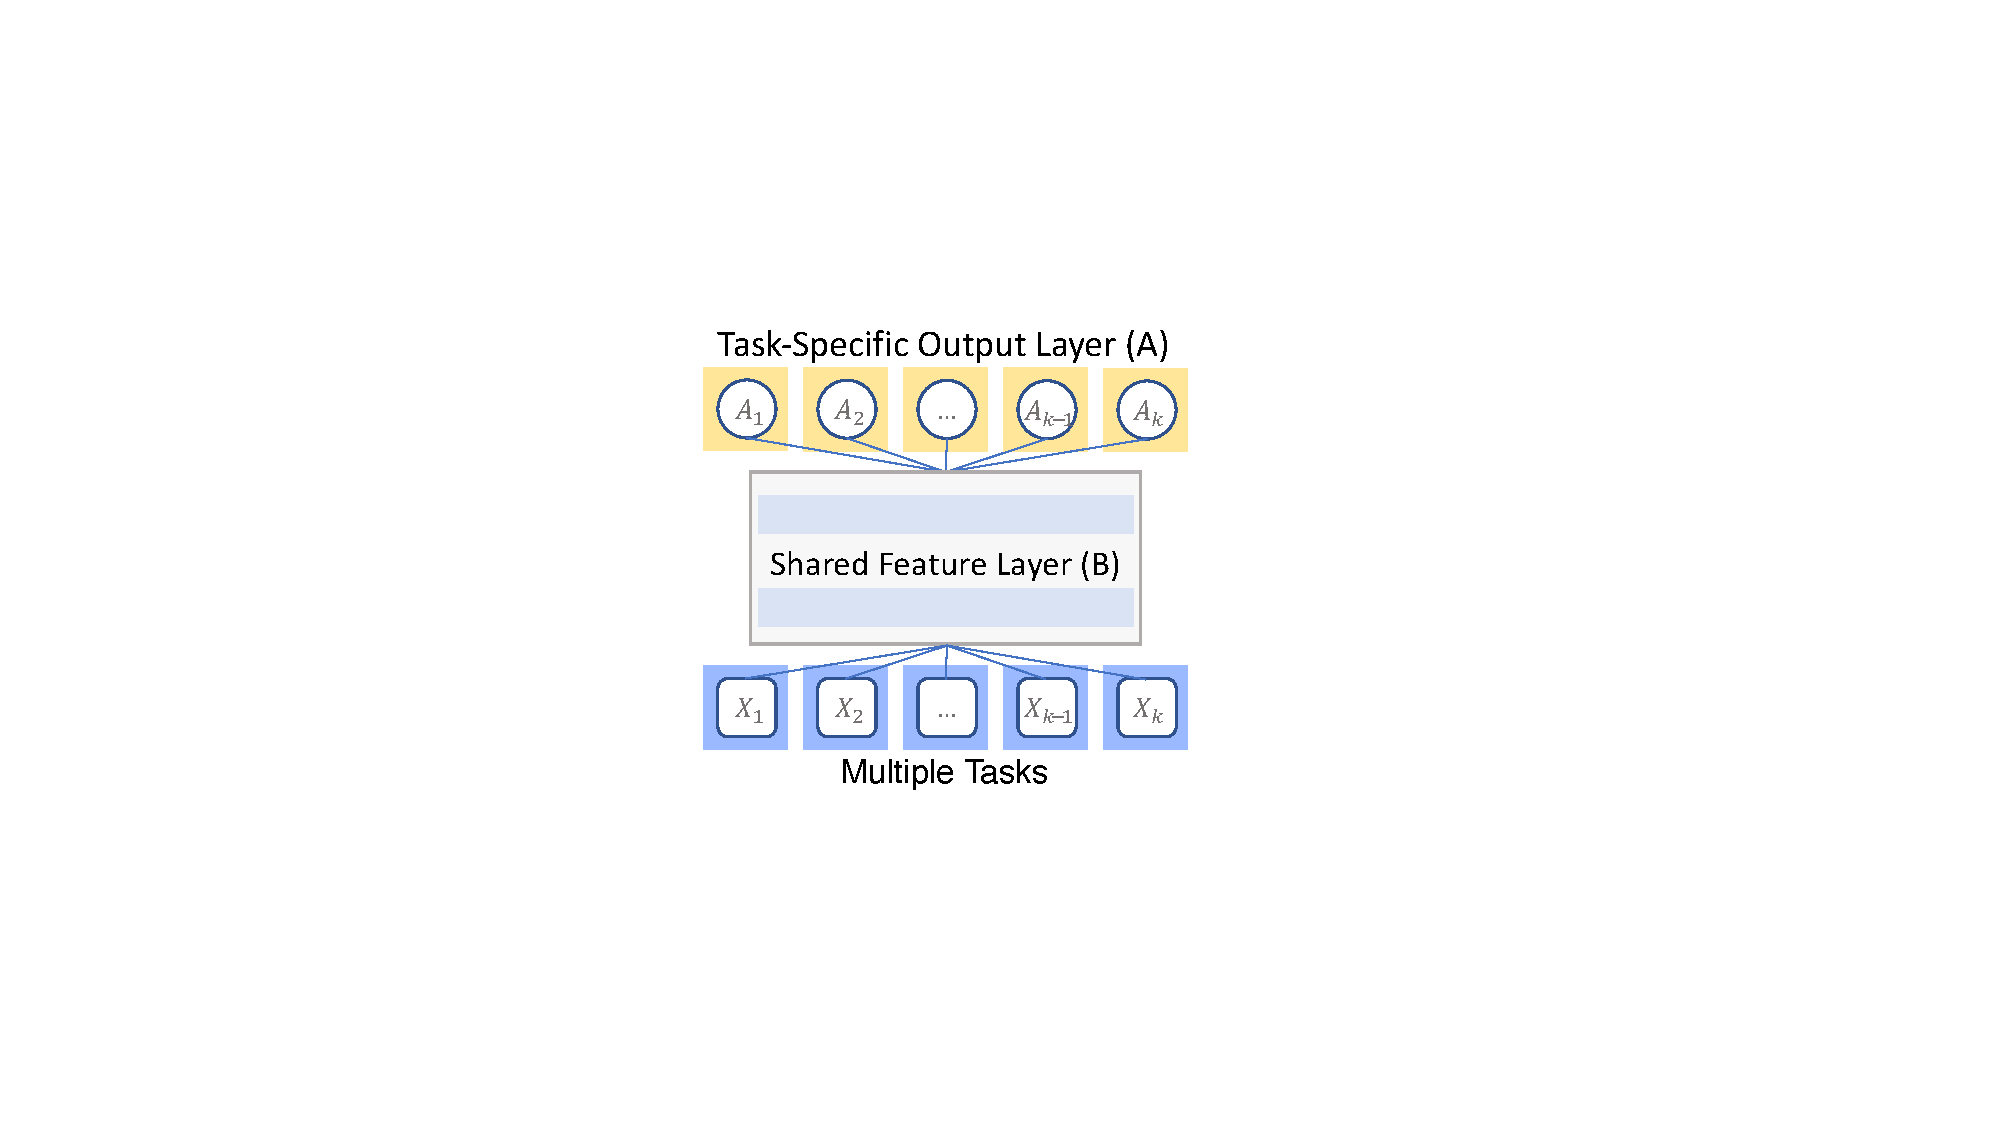
\includegraphics[width=0.5\textwidth,valign=t]{figures/mtl_model_arch.pdf}
		\caption{A hard parameter sharing architecture}
	\end{subfigure}\hfill
	\begin{subfigure}[t]{0.5\textwidth}
		\centering
		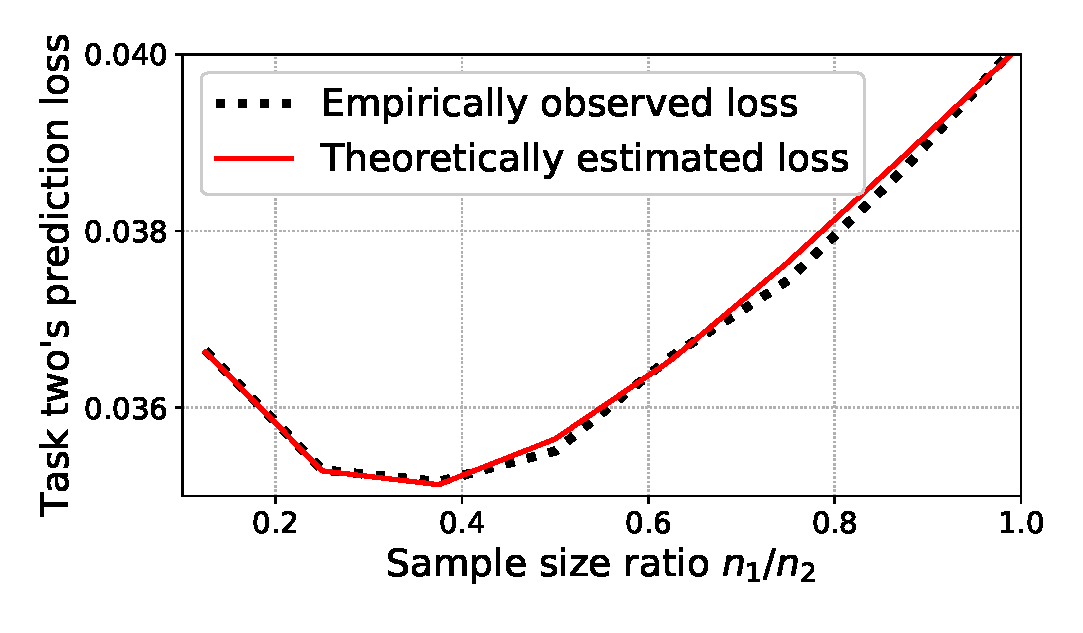
\includegraphics[width=0.713\textwidth,valign=t]{figures/sample_ratio_c2_400.eps}
		\caption{Varying sample size ratio}
		\label{fig_intro_sample_size_b}
	\end{subfigure}
	\caption{An illustrative example of our result:
	Consider the prediction loss of hard parameter sharing (left) for task two, given two linear regression tasks.
	Increasing task one's sample size decreases task two's prediction loss initially, but increases afterward. This phenomenon occurs due to different bias-variance tradeoffs as the sample size ratio increases. Our result provides an estimated loss (solid line) that accurately matches the empirical loss (dotted line).
	See Section \ref{sec_simulation} for the precise setting.}
	\label{fig_intro_sample_size}
\end{figure}

Consequently, we observe qualitative properties of hard parameter sharing for varying datasets' properties using our precise loss estimates.
\begin{enumerate}
	\item \textit{Sample efficiency (Example \ref{ex_same_cov})}:
	One advantage of combining multiple datasets is that the requirement for labeled data reduces compared to STL, a phenomenon that \citet{ZSSGM18} has observed empirically.
	Our results further imply that HPS's sample efficiency depends on model-specific variance vs. noise variance. It is generally high when the noise variance is large compared to model-specific variance across tasks.
	\item \textit{Sample size ratio (Example \ref{ex_sample_ratio})}: Increasing one task's sample size does not always help reduce another task's loss. In a simplified setting, we find that the task loss either decreases first before increasing afterward or decreases monotonically depending on how much bias increases. These two trends result from different tradeoffs between increasing bias and decreasing variance.
	\item \textit{Covariate shift (Example \ref{ex_covshift})}: In addition to sample sizes, variance also scales with the covariate shift between different datasets. For a high sample size ratio, HPS's  variance is smallest when there is no covariate shift. Counterintuitively, for a low sample size ratio, having covariate shifts reduces variance through a complementary spectrum.
\end{enumerate}

%First, we develop tight bounds for the bias and variance of the multi-task estimator for two tasks by applying recent development in random matrix theory \cite{erdos2017dynamical,isotropic,Anisotropic}.
%We observe that the variance of the multi-task estimator is \textit{always smaller} than single-task learning, because of added source task samples.
%On the other hand, the bias of the multi-task estimator is \textit{always larger} than single-task learning, because of model distances.
%Hence, the tradeoff between bias and variance determines whether the transfer is positive or negative.
%We provide a sharp analysis of the \textit{variance} that scales with sample size and covariate shift.
%We extend the analysis to the bias, which \textit{in addition} scales with {task similarity}.
%Combining both, we analyze the bias-variance tradeoff for two tasks in Theorem \ref{thm_main_informal} and extend the analysis to many tasks with the same features in Theorem \ref{thm_many_tasks}.
%For the setting of two tasks, we show how the variance of the multi-task estimator  scales with sample size and covariate shift in the following result.
%\textit{Our first contribution} is to develop a concentration bound that arises naturally from the bias-variance tradeoff of $\hat{\beta}_t^{\MTL}$ for two tasks.
%Let $\hat{\beta}_t^{\STL}$ denote the single-task estimator.
%Without loss of generality, let the $t$-th task denote the target task.
%Importantly, the target task's data size is a fixed constant times $p$ in the high-dimensional setting.
%Hence adding more labeled data can help improve its test performance.
%$B\in\real^{p\times r}$
%$\set{W_i \in \real^{r}}_{i=1}^t$

%Concretely, we show a tight bound on the trace of $(X_1^{\top}X_1 + X_2^{\top}X_2)^{-1}$, which
%Theorem \ref{lem_cov_shift_informal} allows us to analyze the bias-variance tradeoff of the multi-task estimator for two settings:
%(i) two tasks with arbitrary covariate shift; (ii) many tasks with no covariate shift.

%We shall assume that each task data follows a linear model, i.e. $y_i = X_i \beta_i + \varepsilon_i$, $1\le i\le k$.
%Here $\beta_i\in\real^p$ is the model parameter for the $i$-th task.
%Each row of $X_i\in\real^{n_i\times p}$ is assumed to be drawn i.i.d. from a fixed
%distribution with covariance matrix $\Sigma_i$.

%We extend our result to the transfer learning
%in the setting of high-dimensional linear regression.
%by pooling source task representations into the shared body of the hard parameter sharing architecture, following
%setting of Taskonomy by Zamir et al. \cite{ZSSGM18}.
%We prove that the bias of the transfer learning estimator is given by the projection of $\beta_t$ to the orthogonal subspace spanned by $\set{\beta_i}_{i=1}^{t-1}$.
%These results are described more precisely in Section \ref{sec_main}.

%Second, we explain the phenomena in Figure \ref{fig_model_shift_phasetrans} in isotropic and covariate shifted settings.
%We observe that negative transfer occurs as (a) \textit{task similarity}: tasks become more different; (b) \textit{data size}: source/target data size increases.
%\textbf{Task similarity:}
%\textbf{Data sizes:}
%\textbf{Covariate shift:}
%Furthermore, MTL performance is negatively affected when (c) \textit{covariate shift}: the covariance matrices of the two tasks become more different.
%\squishlist
%	\item We provide conditions to predict the effect of transfer as a parameter of model distance $\norm{\beta_1-\beta_2}$ (Section \ref{sec_similarity}).
%	As model distance increases, the bias becomes larger, resulting in negative transfer.
%	Our result predicts most of the empirical observations in Figure \ref{fig_model_shift} correctly.
%	It is crucial that the concentration result in Theorem \ref{lem_cov_shift_informal} is sufficiently precise so that we can explain the transition phenomena in Figure \ref{fig_model_shift} and \ref{fig_size}.
%	The unexplained observations are caused by an error term from the bias.
%	We discuss these in Section \ref{sec_insight}.
%	\item We provide conditions to predict transfer as a parameter of sample ratio $\rho_1/\rho_2$ (Section \ref{sec_data_size}).
%	Adding source task samples helps initially by reducing variance, but hurts eventually due to bias.
	%namely adding more labeled data from the source task does not always improve performance (Proposition \ref{prop_data_size}).
	%Theorem \ref{lem_cov_shift_informal} allows us to compare MTL performance under different covariate shifts.
%	\item For a special case of $\beta_1=\beta_2$, we show that MTL performs best when the singular values of $\Sigma_1^{1/2}\Sigma_2^{-1/2}$ are all equal  (Section \ref{sec_covshift}).
%	Otherwise, the variance reduces less with covariate shift.
%	Our theoretical bound matches the empirical curve in Figure \ref{fig_covariate}.
%\squishend
%In Section \ref{sec_insight}, we consider three components including task similarity, data size and covariate shift for a simplified isotropic setting of two tasks.
%We measure task similarity by how small is the distance between $\beta_1$ and $\beta_2$.
%Using our tool, we explain a transition from positive to negative transfer as task similarity decreases.
%		Furthermore, we show that negative transfer is more likely to occur when the source task labels are particularly noisy.
%		In Section \ref{sec_validate}, we validate the observation on text and image classification tasks.
%	In , we provide the trade-off between $\norm{\beta_1 - \beta_2}^2$ and a certain function $\Phi(\rho_1, \rho_2)$ to determine the type of transfer.
%We show that increasing the data size of the source task does not always improve performance for the target task in multi-task learning.
%Along the way, we analyze the benefit of MTL for reducing labeled data to achieve comparable performance to STL, which has been empirically observed in Taskonomy by Zamir et al. \cite{ZSSGM18}.
%We show that covariate shift, measured by $\Sigma_1^{1/2}\Sigma_2^{-1/2}$, is another cause for suboptimal performance for $\hat{\beta}_t^{\MTL}$.
%		We show that as $n_1 / n_2$ becomes large, having no covariate shift between the source and target tasks yields the optimal performance for the target task.
%		On the other hand, when $n_1 / n_2$ is small, there are counter examples where having the same covariance matrix is not necessarily the optimal choice.

%Our study also leads to several algorithmic consequences with practical interest.
%First, we show that single-task learning results can help to predict positive or negative transfer for multi-task learning.
%We validate this observation on ChestX-ray14 \cite{chexnet17} and sentiment analysis datasets \cite{LZWDA18}.

%Third, we provide a fine-grained insight on a covariance alignment procedure proposed in \cite{WZR20}.
%We show that the alignment procedure provides more significant improvement when the source/target sample ratio is large.
%Finally, we validate our three theoretical findings on sentiment analysis tasks.


There are two main ideas in our analysis. The proof of our first result uses a geometric intuition that hard parameter sharing finds a ``rank-$r$'' approximation of the datasets.
We carefully keep track of the concentration error between the global minimum of $f(A, B)$ and their population version.
The proof of our second result is significantly more involved because of different sample sizes and covariate shifts. Using recently developed techniques from the random matrix theory technique \cite{Anisotropic}, we show that inverse of the sum of two sample covariance matrices with arbitrary covariate shifts converges to a deterministic diagonal matrix asymptotically (cf. Theorem \ref{thm_main_RMT}(i)). % Moreover, we can obtain a sharp bound on the concentration error.
% to obtain a sharp estimate on the..., which is commonly referred to as the \emph{local law}. 
%\HZ{add several sentences on the technical insight} 
One limitation of our analysis is that for two tasks with different sample sizes, there is extra error term in the prediction loss of hard parameter sharing (cf. equation \eqref{cor_MTL_error}), which can be large for very small $n_1$. This requires studying the spectrum of non-symmetric random matrices, which is an intriguing open question (see Section \ref{sec_conclude} for more discussion).
% plus an identity matrix,  due to lack of freeness
%\HZ{add why this is challenging}

Finally, we discuss the practical implications of work.
Our sample size ratio study implies a concrete progressive training procedure that gradually adds more data until performance drops.
For example, in the setting of Figure \ref{fig_intro_sample_size_b}, this procedure will stop right at the minimum of the local basin.
We conduct further studies of this procedure on six text classification datasets and observe that it reduces the computational cost by $65\%$ compared to a standard round-robin training procedure while keeping the average accuracy of all tasks simultaneously.

%This part introduces a positive variance reduction effect from adding the source labels.
%Hence, whether $\te(\hat{\beta}_t^{\MTL}) < \te(\hat{\beta}_t^{\STL})$ is determined precisely by the tradeoff between the negative effect of the bias term and the positive effect of the variance term!
%(i) the negative effect from model shift bias.
%(ii) the positive effect from variance reduction;


\subsection{Related Work}

There is a large body of both classical and recent work on multi-task learning.
We focus our discussion on theoretical works, and refer interested readers to several excellent surveys for general references \cite{PY09,R17,ZY17,V20}.
The early work of \citet{B00,BS03,M06} have sought a study of multi-task learning from a theoretical perspective, often using uniform convergence or Rademacher complexity based techniques.
An influential paper by \citet{BBCK10} provides uniform convergence bounds that combines multiple datasets in certain settings.
One limitation of uniform convergence based techniques is that the results often assume that all  tasks have the same sample size, e.g. \citet{B00,MPR16}.
Secondly, these techniques do not apply to the high-dimensional setting, because the results usually require a sample size at least $p \log p$.

Our proof techniques use the so-called local law of random matrices \cite{erdos2017dynamical}, which is a recent development in the random matrix theory literature.
\citet{isotropic} first proved such a local law for sample covariance matrices with isotropic covariance.
\citet{Anisotropic} later extended this result to arbitrary covariances.
%On the other hand, one may derive the asymptotic result in Theorem \ref{thm_main_RMT} with error $\oo(1)$ using the free addition of two independent random matrices in  theory .
These techniques provide the most sharp convergence rates for the asymptotic limit compared to other techniques such as free probability \cite{nica2006lectures}.
To the best of our knowledge, we are not aware of any previous result for the inverse of the sum of two sample covariance matrices with arbitrary covariate shifts.

The problem we study here is also related to high-dimensional prediction in transfer learning \cite{li2020transfer,bastani2020predicting} and distributed learning \cite{dobriban2018high}.
For example, \citet{li2020transfer} provides minimax optimal rates for predicting a target regression task given multiple sparse regression tasks.
One closely related work is \citet{WZR20}, which studies hard parameter sharing for two linear regression tasks.
\citet{WZR20} (and an earlier work by \citet{KD12}) observed that the shared layer size $r$ in hard parameter sharing plays a critical role of regularization.
%Linear models in multi-task learning have been studied in various settings, including online learning \cite{CCG10,DCSP18}, sparse regression \cite{LPTV09,LPVT11}, and representation learning \cite{BHKL19}.

%Our setting is closely related to domain adaptation \cite{DM06,BB07,BC08,DH09,MMR09,CWB11,ZS13,NB17,ZD19}.
%The important distinction is that we focus on predicting the target task using a hard parameter sharing model.
%For such models, their output dimension plays an important role of regularization \cite{KD12}.
%Below, we describe several lines of work that are most related to this work.

%Some of the earliest works on multi-task learning are Baxter , Ben-David and Schuller \cite{BS03}.
%Mauer \cite{M06} studies generalization bounds for linear separation settings of MTL.
%The benefit of learning multi-task representations has been studied for learning certain half-spaces \cite{MPR16} and sparse regression \cite{LPTV09,LPVT11}.
%Our work is closely related to Wu et al. \cite{WZR20}.
%While Wu et al. provide generalization bounds to show that adding more labeled helps learn the target task more accurately, their techniques cannot be used to explain when MTL outperforms STL.
%\todo{spell out the challenge more explicitly}

%Ando and Zhang \cite{AZ05} introduces an alternating minimization framework for learning multiple tasks.
%Argyriou et al. \cite{AEP08} present a convex algorithm which learns common sparse representations across a pool of related tasks.
%Evgeniou et al. \cite{EMP05} develop a framework for multi-task learning in the context of kernel methods.
%\cite{KD12} observed that controlling the capacity can outperform the implicit capacity control of adding regularization over $B$.
%The multi-task learning model that we have focused on uses the idea of hard parameter sharing \cite{C93,KD12,R17}.
%We believe that our theoretical framework can apply to other approaches to multi-task learning.



\smallskip
\noindent\textbf{Organizations.}
The rest of this paper is organized as follows.
In Section \ref{sec_same}, we present the bias-variance decomposition for hard parameter sharing.
In Section \ref{sec_diff}, we present our technical results for showing how varying sample sizes and covariate shifts impact hard parameter sharing using random matrix theory.
In Section \ref{sec_simulation} and \ref{sec_text}, we validate our theory in both simulations and a real world classification task.
In Section \ref{sec_conclude}, we conclude the paper and describe several open questions.

\paragraph{Notations.}
%Let $\cE \define [\varepsilon_1, \varepsilon_2, \dots, \varepsilon_t] \in \real^{n \times t}$ denote the random noise.
%We can also write $Y = XB^{\star} + \cE$.
%Let $A = [A_1, A_2, \dots, A_t] \in \real^{r\times t}$ be a matrix notation that contains all the output layer parameters.
For a matrix $X$, let $\lambda_{\min}(X)$ denote its smallest singular value and $\norm{X}$ denote its spectral norm.
Let $\lambda_1(X) \ge \lambda_2(X) \ge \cdots \ge \lambda_t(X)$ denote the eigenvalues of $X$.
Let $X^+$ denote its Moore-Penrose psuedoinverse.
We refer to random matrices of the form $\frac {X^\top X} n$ as sample covariance matrices.
We say that an event $\Xi$ holds with high probability if the probability that $\Xi$ happens goes to $1$ as $p$ goes to infinity.
%We shall use $\oo(1)$ to mean a small positive quantity that converges to 0 as $p$ goes to infinity.

%\section{Illustrative Examples}\label{sec_example}


%We provide precise explanations to the phenomena of negative transfer in multi-task learning.
%We provide tight bounds on the bias and variance of the multi-task estimator for two tasks.
%The results in Section \ref{sec_general} show when multi-task learning outperforms single-task learning for general task covariance matrices and ground truth model parameters.
%In particular, the general conditions depend on specific properties of task data such as the covariate shift matrix.
%However, the conditions given by the limiting bias and variance of multi-task learning can be difficult to interpret.
%The goal of this section is to address this issue.
%We interpret the limiting bias and variance equations in an isotropic covariance setting that is described below and a simplified covariate-shifted setting.
%We show that three properties of task data affect the performance of multi-task learning as follows.
%(i) \textit{Task similarity}: We explain the phenomenon of negative transfer precisely as tasks become more different.
%(ii) \textit{Sample ratio}: We further explain a curious phenomenon where increasing the sample ratio between the source and target task helps initially, but hurts eventually.
%(iii) \textit{Covariate shift}: Finally, we show that as the sample size of the source task increases, we show that the covariate shift worsens the performance of the multi-task estimator.
%Finally, we provide a extend our results from two tasks to many tasks with the same features.
%We explain from three perspectives, including \textit{task similarity}, \textit{sample size} and \textit{covariate shift}.
%We show how negative transfer occurs by varying task similarity or sample size.
%Then we show that when source task sample size becomes large, covariate shift causes more negative effects.
We illustrate our main results in simplified settings.
We explain several empirical phenomena that have often been observed when hard parameter sharing approaches are used.

%	The labels are $Y_i = X_i\beta_i + \varepsilon_i$, where $\e_i$ consists of i.i.d. entries with mean zero and variance $\sigma^2$.
%	For our purpose, it is enough to think of the order of $d$ being $1/\sqrt{p}$ and $pd^2/\sigma^2$ being constant.
%The more precise conditions on the relations between $d^2$, $\sigma^2$ and $\kappa^2$ are given in  \eqref{choiceofpara}.
%	We assume that all the random variables have subexponential decay, while keeping in mind that our results can be applied under weaker moments assumptions as shown in Appendix \ref{sec_maintools}.

%In the isotropic model, we show that as we increase the distance between $\beta_1$ and $\beta_2$ (or $d$), there is a transition from positive transfer to negative transfer in MTL.
%We measure model dissimilarity as $\norm{\beta_1 - \beta_2}^2$, which is the distance between source and target in the isotropic model.
%Figure \ref{fig_model_shift} provides a simulation when $p = 200$.
%{The rest of parameter settings can be found in Appendix \ref{app_synthetic}.}
%Our result below will provide an explanation to this phenomenon.
%Based on Theorem \ref{thm_model_shift}, we derive the transition threshold in the following proposition.
%We introduce the following notations.
%{\begin{align*}
%	\Psi(\beta_1, \beta_2) = {\ex{\bignorm{\beta_1 - \beta_2}^2}} / {\sigma^2},  \quad \Phi(\rho_1, \rho_2) = \frac{(\rho_1 + \rho_2 - 1)^2}{\rho_1 (\rho_1 + \rho_2) (\rho_2 - 1)}.
%\end{align*}}


\subsection{Sample Imbalance}

\noindent\textbf{Isotropic features and models.}
	Imagine that we have two tasks and the covariates of both tasks have isotropic covariance matrices.
%	Each task has sample size $n_1 = \rho_1 \cdot p$ and $n_2 = \rho_2 \cdot p$.
	%And $X_1\in\real^{n_1\times p}, X_2\in\real^{n_2\times p}$ denote the covariates of the two tasks, respectively.
	For the ground truth linear model, we consider a random-effects model where the two tasks differ by an independent Gaussian vector.
	Specially, for task two, we assume that its model parameter, denoted by $\beta_2$, consists of i.i.d. Gaussian entries with mean zero and variance $\kappa^2$.
	For task one, we assume that its model parameter, denoted by $\beta_1$, is equal to $\beta_2$ plus i.i.d. Gaussian entries with mean $0$ and variance $d^2$.
	Therefore, the two tasks have different ground truth models. In particular, the distance between $\beta_1$ and $\beta_2$ roughly scales as $d^2 \cdot p$.

%\begin{example}[Varying model distance]
%\end{example}

Using Theorem \ref{thm_main_RMT}, %our techniques described later in Section \ref{sec_general}, 
we can derive the limiting prediction loss of the hard parameter sharing estimator.
Without loss of generality, we describe the result for task two and remark that a similar result for task one holds.

\begin{corollary}[Derived from Theorem \ref{thm_main_RMT}]\label{cor_MTL_loss}
	Assume that the isotropic setting described above holds, and that there exists a small constant $c_0>0$ such that the signal-to-noise ratios satisfy that
\be\label{choiceofpara0}
p^{ c_0} \le \frac{p\kappa^2}{\sigma^2 }  \le p^{1-c_0},\quad  \frac{pd^2}{\sigma^2}=\OO(1).
\ee
	Let $B, W_1, W_2$ be the global minimum of equation \eqref{eq_mtl}. Then with high probability, the prediction loss of the hard parameter sharing estimator for task two satisfies:
	\begin{align}\label{cor_MTL_error}
	%-\left[1- \left( 1-\frac{1}{\sqrt{\rho_1}}\right)^4\right] pd^2\cdot \frac{\rho_1^2 (\rho_1+\rho_2)}{(\rho_1 + \rho_2 - 1)^3} +\OO(p^{-c}\sigma^2)  \le 
	 & \left|L(\hat{\beta}_2^{\MTL}) -\frac{\sigma^2}{\rho_1+\rho_2-1} - pd^2\cdot \frac{\rho_1^2 (\rho_1+\rho_2)}{(\rho_1 + \rho_2 - 1)^3}\right|  \le  \left[\left( 1+\frac{1}{\sqrt{\rho_1}}\right)^4-1\right] pd^2\cdot \frac{\rho_1^2 (\rho_1+\rho_2)}{(\rho_1 + \rho_2 - 1)^3} +\OO(p^{-c}\sigma^2 )
	 \end{align}
	 for any constant $c\in (0,c_0)$.
	 \iffalse
	\begin{align*}
		& \bigabs{ L(\hat{\beta}_2^{\MTL}) - \frac{\sigma^2}{\rho_1 + \rho_2 - 1} - (1 + \frac{6}{\rho_1} + \frac{1}{\rho_1^2})pd^2\cdot \frac{\rho_1^2 (\rho_1+\rho_2)}{(\rho_1 + \rho_2 - 1)^3} } \\
		\le & 	\frac{4}{\sqrt{\rho_1}}(1 + \frac{1}{\rho_1})	pd^2\cdot \frac{\rho_1^2 (\rho_1+\rho_2)}{(\rho_1 + \rho_2 - 1)^3} + \oo(\sigma^2 + pd^2).
%	 \frac{\sigma^2}{\rho_1+\rho_2-1}+\left( 1-\frac{1}{\sqrt{\rho_1}}\right)^4  +\oo(\sigma^2 + pd^2)  \le \\
%	 \le  \frac{\sigma^2}{\rho_1+\rho_2-1}+\left( 1+\frac{1}{\sqrt{\rho_1}}\right)^4 pd^2\cdot \frac{\rho_1^2 (\rho_1+\rho_2)}{(\rho_1 + \rho_2 - 1)^3} +\oo(\sigma^2 + pd^2)
	 \end{align*}
	 \fi
\end{corollary}


It is well-known since the seminal work of Caruana \cite{C97} that how well multi-task learning performs depends on task relatedness. We formalize this connection in the above isotropic setting, where we can perform explicit calculations. The prediction loss of MTL has been given in Corollary \ref{cor_MTL_loss}. We can also calculate the prediction loss of STL easily using Fact \ref{lem_minv} (ii). The proof of the following claim will be given in Section \ref{app_iso_cov}.
\begin{claim} \label{claim_STL_loss}
Under the above isotropic setting for task two, we have that with high probability,
\begin{align*}
	 L(\hat{\beta}_2^{\STL}) = \frac{\sigma^2}{ \rho_2-1}  +\OO(p^{-\e}\sigma^2 )
	 \end{align*}
	 for any constant $\e\in (0,1/2)$.
\end{claim}

We now discuss two implications of Corollary \ref{cor_MTL_loss} and Claim \ref{claim_STL_loss} regarding the information transfer in MTL: the transitions from positive transfer to negative transfer with respect to varying model distance and varying sample ratio, respectively.

\medskip

\noindent{\bf Varying model distance.} 
%With Corollary \ref{cor_MTL_loss} and Claim \ref{claim_STL_loss}, it is not hard to see 
One can observe that as we increase the distance $pd^2$ between $\beta_1$ and $\beta_2$, there is a transition from positive transfer to negative transfer in MTL. More precisely, the bias term $  pd^2\cdot \frac{\rho_1^2 (\rho_1+\rho_2)}{(\rho_1 + \rho_2 - 1)^3}$ of MTL increases as the distance between $\beta_1$ and $\beta_2$ increases, while variance reduction from STL to MTL is $\frac{\sigma^2}{ \rho_2-1}  -\frac{\sigma^2}{\rho_1+\rho_2-1}$.
%Therefore, while the variance of MTL still reduces compared to STL, 
If the bias increases more than the amount of variance reduced, we will observe negative transfer.

\iffalse
\begin{proposition}[Task model distance]\label{prop_dist_transition}
	In the isotropic model, suppose that $\rho_1$ and $\rho_2 > 1$.
	Then
	%Whether $\te(\hat{\beta}_t^{\MTL})$ is lower than $\te(\hat{\beta}_t^{\STL})$ is determined by the ratio between $\Psi(\beta_1, \beta_2)$ and $\Phi(\rho_1, \rho_2)$:
	\begin{itemize}
		\item \textbf{Positive transfer:} If $\Psi(\beta_1, \beta_2) < \frac{1}{\nu} \cdot  \Phi(\rho_1, \rho_2)$, then w.h.p. over the randomness of $X_1,X_2$,
			\[ \te(\hat{\beta}_2^{\MTL}) < \te(\hat{\beta}_2^{\STL}). \]
		\item \textbf{Negative transfer:} If $\Psi(\beta_1, \beta_2) > {\nu} \cdot  \Phi(\rho_1, \rho_2)$, then w.h.p. over the randomness of $X_1,X_2$,
			$$\te(\hat{\beta}_2^{\MTL}) > \te(\hat{\beta}_2^{\STL}).$$
	\end{itemize}
	Here {\small$\nu = (1+\oo(1)) \cdot (1 - 1/\sqrt{\rho_1})^{-4}$}.
	Concretely, if $\rho_1 > 40$, then $\nu\in (1,2)$.
\end{proposition}
Proposition \ref{prop_dist_transition} simplifies Theorem \ref{thm_main_informal} in the isotropic model, allowing for a more explicit statement of the bias-variance tradeoff.
Concretely, $\Psi(\beta_1, \beta)$ and $\Phi(\rho_1, \rho_2)$ corresponds to $\Delta_{\bias}$ and $\Delta_{\vari}$, respectively.
%Roughly speaking, the transition threshold scales as $\frac{pd^2}{\sigma^2} - \frac{1}{\rho_1} - \frac{1}{\rho_2}$.
\fi

We apply Corollary \ref{cor_MTL_loss} and Claim \ref{claim_STL_loss} to the parameter setting of Figure \ref{fig_model_shift} (the details are left to Appendix \ref{app_synthetic}). We can see that our result is able to predict positive or negative transfer  accurately and matches the empirical curve.
There are several unexplained observations near the transition threshold $0$, which are caused by the concentration error on the right-hand side of \eqref{cor_MTL_error}.
%We fix the target task and vary the source task, in particular the parameter $d$ which determines $\norm{\beta_1 - \beta_2}$.
%Figure \ref{fig_model_shift} shows the result.
%We observe that Proposition \ref{prop_dist_transition} explains most of the observations in Figure \ref{fig_model_shift}.

\iffalse
The proof of Proposition \ref{prop_dist_transition} involves two parts.
First, in equation \eqref{eq_te_var}, the positive variance reduction effect scales with $n_1 = \rho_1 p$, the number of source task data points.
Second, we show that the negative effect of model-shift bias scales with $pd^2$, which is the expectation of $\norm{\beta_1 - \beta_2}^2$.
The proof of Proposition \ref{prop_dist_transition} can be found in Appendix \ref{app_proof_31}.
A key part of the analysis shows that $\hat{W}_1 / \hat{W}_2$ is roughly equal to one in the isotropic model,
thus simplifying the general condition in Theorem \ref{thm_main_informal}.
\fi

\begin{figure}[!t]
	\begin{subfigure}[b]{0.32\textwidth}
		\centering
		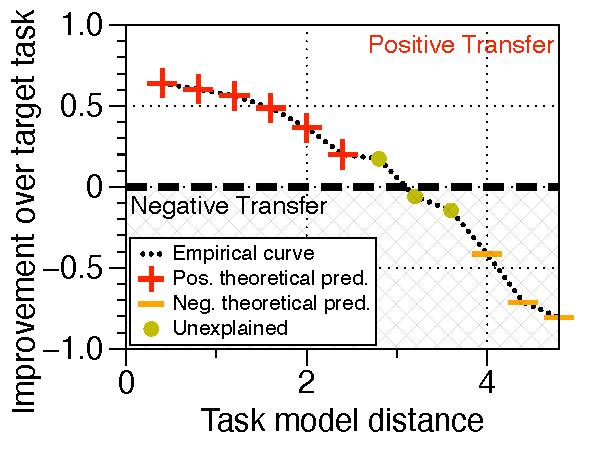
\includegraphics[width=0.98\textwidth]{figures/model_shift_phase_transition.pdf}
		\caption{Task similarity}
		\label{fig_model_shift}
	\end{subfigure}\hfill
	\begin{subfigure}[b]{0.32\textwidth}
		\centering
		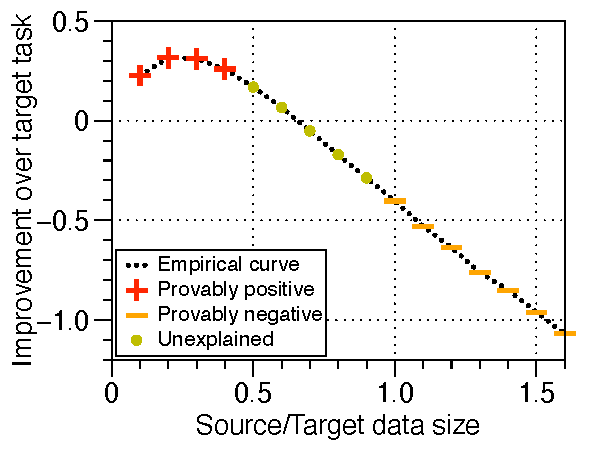
\includegraphics[width=0.98\textwidth]{figures/datapoints_phase_transition.pdf}
		\caption{Sample size}
		\label{fig_size}
	\end{subfigure}\hfill
	\begin{subfigure}[b]{0.32\textwidth}
		\centering
		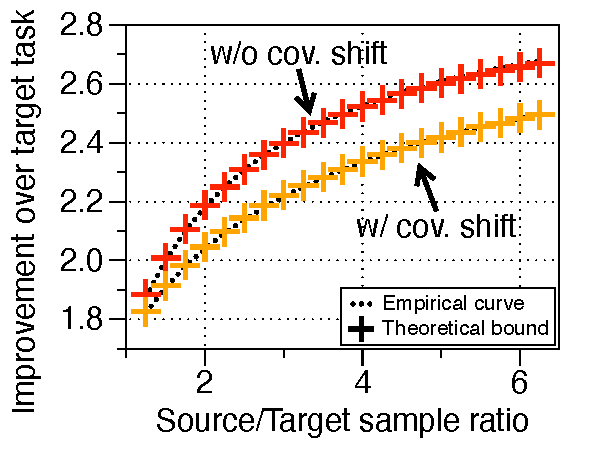
\includegraphics[width=0.98\textwidth]{figures/complementary.pdf}
		\caption{Covariate shift}
		\label{fig_covariate}
	\end{subfigure}
	\caption{%Three takeaways of our theory in Section \ref{sec_insight}.
	We observe a transition from positive to negative transfer as (a) \textit{task model distance} increases and (b) source/target \textit{sample ratio} increases.
	For the special case of having the same task model, we observe in (c) that as source/target \textit{sample ratio} increases, having \textit{covariate shift} worsens the performance of MTL.
	The $y$-axis measures the loss of STL minus MTL.}
	\label{fig_model_shift_phasetrans}
\end{figure}

%\subsection{Sample Ratio}\label{sec_data_size}

\medskip
\noindent{\bf Varying sample ratio.} In classical Rademacher or VC based theory of multi-task learning, the generalization bounds are usually presented for settings where the sample sizes are equal for all tasks \cite{B00,M06,MPR16}.
%More generally, such results are still applicable when all task data are being added simultaneously.
On the other hand, uneven sample sizes between different tasks (or even dominating tasks) have been empirically observed as a cause of negative transfer \cite{YKGLHF20}.
For such settings, we have also observed that adding more labeled data from one task does not always help.
Our theory accurately predicts a curious phenomenon, where increasing the sample size of the source task results in negative transfer!
%On the other hand, we have observed that adding more labeled data does not always improve performance in multi-task learning.

More precisely, in the isotropic model, we consider what happens if we vary the source task sample size. For fixed model distance $pd^2$, the bias term $  pd^2\cdot \frac{\rho_1^2 (\rho_1+\rho_2)}{(\rho_1 + \rho_2 - 1)^3}$ of MTL increases and converges to $pd^2$ as the sample ratio $\rho_1/\rho_2$ increases, and the variance reduction $\frac{\sigma^2}{ \rho_2-1}  -\frac{\sigma^2}{\rho_1+\rho_2-1}$ also increases and converges to $\frac{\sigma^2}{\rho_2-1}$ as $\rho_1/\rho_2$ increases. The tradeoff between these two terms depends on $\rho_1$ in a nonlinear way that is more complicated than the one in the case of varying model distance. But from our results, one can check the following phenomena. If $\frac{\sigma^2}{\rho_2-1} > pd^2$, then the transfer is always positive. On the other hand, if $\frac{\sigma^2}{\rho_2-1} < pd^2$, then there is a transition from the positive transfer to negative transfer as $\rho_1/\rho_2$ increases. 
%Therefore, while the variance of MTL still reduces compared to STL, 
%If the bias increases more than the amount of variance reduced, we will observe negative transfer.
Figure \ref{fig_size} provides a simulation result for such a setting (described in Appendix \ref{app_synthetic}).
%We observe that as $n_1 / n_2$ increases, there is a transition from positive to negative transfer. 
There are several unexplained observations near $y = 0$ caused by the concentration error on the right-hand side of \eqref{cor_MTL_error}.


\iffalse
\begin{proposition}[Source/target sample ratio]\label{prop_data_size}
	In the isotropic model, suppose that $\rho_1 > 40$ and $\rho_2 > 110$ are fixed constants, and $\Psi(\beta_1, \beta_2) > 2/(\rho_2 - 1)$.
	Then we have that
	\begin{itemize}
		\item \textbf{Positive transfer:} If $\frac{n_1}{n_2} = \frac{\rho_1}{\rho_2} < \frac{1}{\nu} \cdot \frac{1 - 2\rho_2^{-1}}{\Psi(\beta_1, \beta_2) (\rho_2 - 1) - \nu^{-1}}$, then w.h.p. $$\te(\hat{\beta}_2^{\MTL}) < \te(\hat{\beta}_2^{\STL}).$$
		\item \textbf{Negative transfer:} If $\frac{n_1}{n_2} = \frac{\rho_1}{\rho_2} > {\nu} \cdot \frac{1 - 2\rho_2^{-1}}{\Psi(\beta_1, \beta_2) (\rho_2 - 3/2) - \nu}$, then w.h.p. $$\te(\hat{\beta}_2^{\MTL}) > \te(\hat{\beta}_2^{\STL}).$$
	\end{itemize}
\end{proposition}
Proposition \ref{prop_data_size} describes the bias-variance tradeoff in terms of the sample ratio $\rho_1 / \rho_2$.


We apply the result to the setting of Figure \ref{fig_size} (described in Appendix \ref{app_synthetic}).
There are several unexplained observations near $y = 0$ caused by $\nu$.
The proof of Proposition \ref{prop_data_size} can be found in Appendix \ref{app_proof_32}.
\fi

\subsection{Covariate Shift} \label{sec_covshift}
So far we have considered the isotropic model where $\Sigma_1 = \Sigma_2$.
This setting is relevant for settings where different tasks share the same input features such as multi-class image classification.
In general, the covariance matrices of the two tasks may be different such as in text classification.
In this part, we consider what happens when $\Sigma_1 \neq \Sigma_2$.
We show that when $n_1 / n_2$ is large, MTL with covariate shift can be suboptimal compared to MTL without covariate shift.

%\noindent\textit{Example.}

\begin{example}
	We measure covariate shift by the transfer matrix $M = \Sigma_1^{1/2} \Sigma_2^{-1/2}$. %similar to Theorem \ref{thm_main_informal}.
	We assume that the two tasks have the same ground truth model parameters, that is, $\beta_1 = \beta_2$.
	We compare two cases: (i) when $M = \id_{p\times p}$; (ii) when $M$ has $p/2$ singular values that are equal to $\lambda$ and $p/2$ singular values that are equal to $1 / \lambda$.
	Hence, $\lambda$ measures the severity of the covariate shift.
	Figure \ref{fig_covariate} shows a simulation of this setting by varying $\lambda$.
	We observe that as source/target sample ratio increases, the performance gap between the two cases increases.
	\end{example}

%By applying Lemma \ref{lem_cov_shift_informal}, we find that when $n_1 / n_2$ is large, having no covariate shift is the optimal choice provided that the determinant of $M^{\top}M$ is bounded.
We compare different choices of $M$ that belong to the following bounded set.
Let $\lambda_i$ be the $i$-th singular value of $M$.
Let $\mu_{\min} < \mu < \mu_{\max}$ be fixed values that do not grow with $p$.
{\begin{align*}
		\cS_{\mu}\define\bigset{M \left| \prod_{i=1}^p \lambda_i \le \mu^p, \mu_{\min} \le \lambda_i\le \mu_{\max}, \text{ for all } 1\le i\le p\right.}.
\end{align*}}
%	We assume that $\beta_1$ and $\beta_2$ are generated following the isotropic model with $d = 0$.
\begin{proposition}[Covariate shift]\label{prop_covariate}
	For the setting of the example above, assume that $\beta_1 = \beta_2$, $\rho_1$ and $\rho_2$ are both greater than one.
	Let $g(M)$ denote the prediction loss of $\hat{\beta}_t^{\MTL}$ when $M = \Sigma_1^{1/2}\Sigma_2^{-1/2} \in\cS_{\mu}$.
	We have that
		\[ g(\mu\id) \le \bigbrace{1+ \bigo{{\rho_2}/{\rho_1}  }} \min_{M\in\cS_{\mu}} g(M). \]
\end{proposition}


\iffalse

 \begin{claim}\label{claim_covar_shift}
		In the setting of Proposition \ref{prop_covariate}, for any $M\in \cal S_\mu$ we have that
		\[ g(M)=(1+\OO(p^{-\e}))\cdot \sigma^2  \bigtr{\Sigma_2(X_1^{\top}X_1  + X_2^{\top}X_2)^{-1} }  \quad \text{w.h.p.} \]
	\end{claim}

%Finally, in this subsection we prove Proposition \ref{prop_covariate}, which shows that $\te(\hat{\beta}_2^{\MTL})$ is minimized approximately when $M$ is a scalar matrix, provided that there is enough source data.

\begin{proof}[Proof of Proposition \ref{prop_covariate}]
 

 
 Denote the minimizer of $g$ by 
$$M_0:=\argmin_{M\in \cal S_{\mu}}g(M).$$ 
We now calculate $g(M_0)$. 


Now using Lemma \ref{lem_cov_shift}, we obtain that with high probability,
\begin{align}\label{gvar_extra}
g(M_0)= \frac{\sigma^2}{\rho_1+\rho_2}\cdot \frac1p\tr\left( \frac{1}{a_1(M_0)\cdot M_0^\top M_0 + a_2(M_0)}\right) \cdot \left(1 +\OO(p^{-\e})\right).
\end{align}
From equation \eqref{eq_a12extra}, it is easy to obtain the following estimates on $ a_1(M)$ and $a_2(M)$ for any $M\in \cal S_\mu$:
\be\label{est_a12extra}
\frac{\rho_1-1}{\rho_1+\rho_2} < a_1(M)<  \frac{\rho_1+\rho_2-1}{\rho_1+\rho_2},\quad a_2(M) < \frac{\rho_2}{\rho_1+\rho_2}.
\ee
Inserting \eqref{est_a12extra} into \eqref{gvar_extra} and using $ M_0^\top M_0\succeq \mu_{\min}^2$, we obtain that with high probability,
\begin{align}\label{approximateteM}
\left(1+\frac{\rho_2}{(\rho_1-1)\mu_{\min}^2}\right)^{-1}h(M_0) \cdot \left(1 - \OO(p^{-\e})\right) \le g(M_0) \le h(M_0) \cdot \left(1 +\OO(p^{-\e})\right),
\end{align}
where
$$h(M_0):=\frac{\sigma^2}{(\rho_1+\rho_2)a_1(M_0)}\cdot \frac1p\tr\left( \frac{1}{M_0^\top M_0}\right) .$$
%With these two bounds, we can easily conclude \eqref{approxteM}. 
%
%We have that the test error satisfies
%\be\label{approxteM}  te(M)\left(1 -  \frac{n_2}{n_1-p} \frac{1}{\lambda_p^2 + \frac{n_2}{n_1-p}}\right)  \le  \frac{\sigma^2}{n_1+n_2}\tr\left( \frac{1}{a_1M^\top M + a_2}\right) \le te(M),\ee
%where $\lambda_p$ is the smallest singular value of $p$ and
%$$te(M):= \frac{\sigma^2}{a_1(n_1+n_2)}\tr\left( \frac{1}{M^\top M}\right) .$$
%Moreover, for all $M$ satisfying \eqref{GMcons}, the minimum of $te(M)$ is attained when $M= a\id$.
By AM-GM inequality, we observe that 
$$\tr\left( \frac{1}{M^\top M}\right) = \sum_{i=1}^p\frac{1}{\lambda_i^2}$$
is minimized when $\lambda_1 = \cdots\lambda_p=\mu$ under the restriction $\prod_{i=1}^p\lambda_i\le \mu^p$. Hence we get that 
\be\label{AMGM} h(M_0) \le \frac{\sigma^2}{\mu^2 (\rho_1+\rho_2)a_1(M_0)}.\ee
On the other hand, when $M=\mu \id$, applying Lemma \ref{lem_cov_shift} we obtain that with high probability,
\begin{align}\label{gvar_extra2}
\begin{split}
g(\mu \id)&= \frac{\sigma^2}{\rho_1+\rho_2}\cdot \frac1p\tr\left( \frac{1}{\mu^2 a_1 (\mu\id) + a_2(\mu\id)}\right) \cdot \left(1 +\OO(p^{-\e})\right)\\
&\le \frac{\sigma^2}{\mu^2(\rho_1+\rho_2)a_1 (\mu\id)}.
\end{split}
\end{align}
Combining \eqref{est_a12extra}, \eqref{approximateteM}, \eqref{AMGM} and \eqref{gvar_extra2}, we conclude the proof.
%, we conclude that the sum $\sum_{i=1}^p\lambda_i^{-1}$ is smallest when $\lambda_1=\cdots=\lambda_p = a$.
\end{proof}
\fi

Proposition \ref{prop_covariate} shows that when the sample ratio is large, having no covariate shift gives the optimal performance for multi-task learning.
The proof of Proposition \ref{prop_covariate} can be found in Appendix \ref{app_proof_33}.
%Proposition \ref{prop_covariate} implies that when $\rho_1\gg \rho_2$, having no covariate shift is the optimal choice for choosing the source task.
%This provides evidence that covariate shift is unfavorable when there are many source task datapoints,

%\todo{} To complement the result, we show an example when the statement is not true if $n_1 \le n_2$.

%We ask: is it better to have $M$ as being close to identity, or should $M$ involve varying levels of singular values?
%Understanding this question has implications for applying normalization methods in multi-task learning \cite{LV19,CBLR18,YKGLHF20}.
%We show that if $n_1$ is much larger than $n_2$, then the optimal $M$ matrix should be proportional to identity, under certain assumptions on its range of singular values (to be formulated in Proposition \ref{prop_covariate}).
%On the other hand, if $n_1$ is comparable or even smaller than $n_2$, we show an example where having ``complementary'' covariance matrices is better performing than having the same covariance matrices.



\subsection{Sample Efficiency}

observed in Taskonomy \cite{ZSSGM18}.



\section{A Bias-variance Decomposition for Multiple Tasks}\label{sec_same}

%We begin by considering the case where all tasks have the same sample size and feature covariates, that is, $n_i = n$ and $X^{(i)} = X\in\real^{n\times p}$ for all $i = 1, \dots, t$.
%We provide a sharp generalization error bound of hard parameter sharing estimators.
We show that the prediction loss of hard parameter sharing admits a clean bias-variance decomposition, when all tasks have the same sample size and feature covariates.
%This setting is prevalent in applications of multi-task learning to image classification, where there are multiple prediction labels/tasks for every image \cite{chexnet17,EA20}.
%We consider an arbitrary local minimum $B, W_1, \dots, W_2$ of the optimization objective.
%We extend the bias-variance decomposition from the two-task case to the multiple-task case.
%We observe that the expected prediction loss of $\hat{\beta}_t^{\MTL}$ conditional on $X$ consists of a bias and a variance equation as follows
%\begin{align}
%	\exarg{\varepsilon_1, \dots, \varepsilon_t}{L(\hat{\beta}_t^{\MTL}) \mid X}
%	=& \bignorm{\Sigma^{1/2} \bigbrace{B^{\star} \cW^{\top} (\cW \cW^{\top})^{-1} W_t - \beta_t}}^2 \label{eq_bias_multiple} \\
%	&+ \sigma^2 \cdot (W_t^{\top} (\cW \cW^{\top})^{-1} W_t) \cdot \bigtr{\Sigma (X^{\top} X)^{-1}} \label{eq_var_multiple}
%\end{align}
%One can see that equation \eqref{eq_bias_multiple} is the bias of the multi-task learning estimator and equation \eqref{eq_var_multiple} is its variance.
%Compared to the prediction loss of single-task learning (cf. equation \eqref{eq_var_stl}), we observe that the variance equation \eqref{eq_var_multiple} is always smaller because $W_t^{\top} (\cW \cW^{\top})^{-1} W_t \le 1$.
%On the other hand, the bias equation \eqref{eq_bias_multiple} is always larger because of the difference between the task models.
%We show the generalization error of hard parameter sharing estimators.
%Before stating the result, we define the following notations.
Let $\Sigma$ denote the population covariance matrix of all tasks.
Suppose we have $t$ tasks $(X, Y^{(1)})$, $(X, Y^{(2)})$, \dots, $(X, Y^{(t)})$ where $X = Z \Sigma^{1/2} \in\real^{n\times p}$ and $Y^{(i)} = X \beta^{(i)} + \varepsilon^{(i)}$:
every entry of $Z \in \real^{n \times p}$ is drawn independently from a one dimensional distribution with mean zero, unit variance, and constant $\varphi$-th moment for $\varphi > 4$;
every entry of $\cE \in \real^{n \times t}$ is drawn indepdently from a one dimensional ditribution with mean zero, variance $\sigma^2$, and bounded moment up to any order.\footnote{More precisely, there exists a fixed function $C: \mathbb{Z} \rightarrow \real^+$ such that for any $k = 2, 4, \dots, \infty$, the $k$-th moment is bounded by $C(k)$.}
Let $A^{\star} {A^{\star}}^{\top}$ denote the best rank-$r$ subspace approximation of ${B^{\star}}^\top\Sigma B^{\star}$, that is,
\[ A^{\star} \define \argmin_{U\in\real^{t\times r} : U^{\top} U = \id_{r\times r}} \inner{U U^{\top}} {{B^{\star}}^{\top} \Sigma B^{\star}}. \]
Let $\lambda_1({B^\star}^\top \Sigma B^\star)\ge\lambda_2({B^\star}^\top \Sigma B^\star)\ge \cdots \ge \lambda_t({B^\star}^\top \Sigma B^\star)$ be the eigenvalues of ${B^\star}^\top \Sigma B^\star$. To ensure that $A^{\star}$ is unique, we assume that the $\lambda_{r+1}({B^\star}^\top \Sigma B^\star)$ is smaller than $\lambda_{r}({B^\star}^\top \Sigma B^\star)$.
For $i = 1,\dots, t$, let $a_i^{\star} \in\real^r$ denote the $i$-th column of $A^{\star}{A^{\star}}^{\top}$. 
Our main result shows that hard parameter sharing essentially approximates all tasks through the rank-$r$ matrix $B^{\star} A^{\star} {A^{\star}}^{\top}$.

\begin{theorem}[Bias-variance decomposition for prediction loss]\label{thm_many_tasks}
%Suppose $X=Z\Sigma^{1/2}\in \R^{n\times p}$ satisfy Assumption \ref{assm_secA1} with $\rho:=n/p>1$ being some fixed constant. Consider data models  $Y_i = X\beta_i + \varepsilon_i$, $i=1,2,\cdots, t$, where $\e_i\in \R^{n}$ are random vectors with i.i.d. entries with mean zero, variance $\sigma^2$ and all moments as in \eqref{assmAhigh}. Moreover, assume that $X$, $\beta_i$ and $\e_i$ are all independent of each other.
	%Let $n = c \cdot p$.
	%Let $X\in\real^{n\times p}$ and $Y_i = X\beta_i + \varepsilon_i$, for $i = 1,\dots,k$.
%	Consider $t$ data models $Y_i = X\beta_i + \varepsilon_i$, $i=1,2,\cdots, t$, where $X$ has covariance matrix $\Sigma$, and the entries of $\e_i$ are i.i.d. with mean zero and variance $\sigma^2$.gT
	%that satisfy Assumption \ref{assm_secA2} in the appendix.
	Assume that $n > \rho p$ for a fixed constant $\rho > 1$.
	Let $c_{\varphi}$ be any fixed value within $(0, \frac{\varphi-4}{2\varphi})$.
	Let $L(B^{\star}a_i^{\star}): = \norm{\Sigma^{1/2} (B^{\star} a_i^{\star}- \beta^{(i)})}^2$.
	For any task $i = 1, 2, \dots, t$, the prediction loss of the estimator $\hat{\beta}_i^{\MTL}$ satisfies that with high probability,
	\begin{align*}
		\bigabs{L(\hat{\beta}_i^{\MTL}) - L(B^{\star}a_i^{\star}) - \sigma^2 \norm{a_i^{\star}}^2 \bigtr{\Sigma (X^{\top}X)^{-1}}}
		\le n^{-c_{\varphi}/2} \cdot C_1\bigbrace{ \norm{\Sigma^{1/2} B^{\star}}^2+  \sigma^2}  ,
	\end{align*}
	where $C_1: = \frac{\bignormFro{\Sigma^{1/2} B^{\star}}^2 + \sigma^2 t}{\lambda_r ({B^\star}^\top \Sigma B^\star)- \lambda_{r+1}({B^\star}^\top \Sigma B^\star)}$ and $C_2 :=  C_1\cdot \norm{\Sigma^{1/2} B^{\star}}$.
\end{theorem}

%\FY{why not use $C_1: = \frac{ \normFro{\Sigma^{1/2} B^{\star}}^2}{ \lambda_{\min}^2(\Sigma^{1/2} B^{\star}) + \sigma^2}$? $C_2$ does not seem to be correct because the dimension does not match. I will check the proof to see whether $C_2 =  C_1\cdot \norm{\Sigma^{1/2} B^{\star}}^2$ or $C_1\cdot \sigma\norm{\Sigma^{1/2} B^{\star}}$?}
Theorem \ref{thm_many_tasks} provides a sharp generalization error bound that is asymptotically tight when $p$ goes to infinity.
The limiting loss of hard parameter sharing consists of two parts, a bias term $L(B^{\star} a_i^{\star})$ that measures the error of $B^{\star} a_i^{\star}$, and a variance term that scales with noise variance $\sigma^2$.
%	Our result implies that the variance of hard parameter sharing is always smaller than single-task learning.
%	This is because	STL's variance is equal to $\frac{\sigma^2 \cdot p} {n - p}$ by Fact \ref{lem_minv}, and $\norm{a_i^{\star}}^2 \le 1$ since the spectral norm of $U_r$, which is a projection matrix, is at most one.
We can compare how well hard parameter sharing performs vs. single-task learning, whose prediction loss is equal to $\sigma^2 \tr[\Sigma (X^{\top} X)^{-1}]$, for every task $i$.
On one hand, hard parameter sharing helps by reducing variance, since $\norm{a_i^{\star}}^2 \le 1$.
On the other hand, it hurts by increasing bias.


\paragraph{How does hard parameter sharing scale with sample size $n$?}
We first consider the variance term.
Intuitively, variance reduces as $n$ increases.
To make this precise, we introduce the high-dimensional setting that assumes $n / p$ increases at a fixed ratio.
\begin{assumption}\label{assume_rm}
	Let $\tau > 0$ be a small enough constant.
%	Let $X = Z \Sigma^{1/2} \in\real^{n\times p}$ be a random matrix where $Z \in \real^{n\times p}$ consists of i.i.d. entries with zero mean and unit variance and $\Sigma \in \real^{p\times p}$ is a positive semidefinite matrix.
	In the high-dimensional setting,
%		\item For every entry of $Z$, we assume that its $\varphi$-th moment exists, that is, there exist a fixed constant $C > 0$ such that
%			\begin{align}\label{assmAhigh}
%				\ex{\abs{Z_{i,j}}^{\varphi}} \le C, \text{ for any } 1\le i \le n \text{ and } 1\le j \le p.
%			\end{align}
  the sample size $n$ grows to infinity proportionally with the dimension $p$, i.e. $n / p \rightarrow \rho \in (\tau, 1/\tau)$ as $p$ goes infinity.
%	\end{enumerate}
\end{assumption}
Under the above assumption, we state a well-known fact for $\tr[\Sigma (X^{\top} X)^{-1}] = \tr[(Z^{\top} Z)^{-1}]$.

\begin{fact}[cf. Theorem 2.4 in \citet{isotropic}]\label{fact_tr}
	%Let $X  \in \real^{n\times p}$ be a random matrix that satisfies Assumption \ref{assume_rm}.
	%Let $\Sigma\in\real^{p\times p}$ denote the population covariance matrix of $X$.
	With high probability over the randomness of $Z$, we have that $\bigtr{\Sigma (X^{\top} X)^{-1}} = \frac{p}{n - p} + \OO(p^{-c_{\varphi}})$.
\end{fact}

%Finally, for the random noise component, we assume that all of its moments exist.
%More precisely, there exists a fixed function $C(\cdot) : \mathbb{Z} \rightarrow \real^+$ such that for any $a = 1, 2, \dots, \infty$, we have that
%\begin{align}\label{assmAhigh2}
%	\ex{\abs{\varepsilon_{j}^{(i)}}^a} \le C(a), \text{ for any } 1\le i\le t \text{ and } 1\le j\le n_i.
%\end{align}
%Hence, for any value $\varphi > 4$, we get that Fact \ref{lem_minv} holds for $\varepsilon^{(i)}$, for all $i = 1, 2, \dots, t$.
%Let $\e$ be a small enough fixed value and let $c_{\infty}$ be any fixed value within $(0, 1/2-\e)$.
%We have that Fact \ref{lem_minv} holds for $\varepsilon^{(i)}$ where $c_{\varphi}$ becomes $c_{\infty}$ instead.

Next, we consider the bias $L(B^{\star} a^{\star}_i)$.
We illustrate through a random-effects model, which has been studied for a single task \cite{dobriban2020wonder}.
Suppose every $\beta_i$ consists of two random components, one that is shared among all tasks and one that is task-specific.
Thus, each task contributes a certain amount to the shared component and injects a task-specific bias.
Let $\beta_0$ denote the shared component whose entries are sampled i.i.d. from an isotropic Gaussian distribution of mean zero and variance $p^{-1}\kappa^2$.
Let the task-specific component be a random Gaussian vector whose coordinates all have mean zero and variance $p^{-1} d^2 / 2$.
Thus, for any two different $\beta_i$ and $\beta_j$, their distance is roughly $d^2$.
%	The labels are $Y_i = X_i\beta_i + \varepsilon_i$, where $\e_i$ consists of i.i.d. entries with mean zero and variance $\sigma^2$.
Concretely, we can think of $\kappa = 1$ and $d^2/\sigma^2 \le \OO(1)$.
%The more precise conditions on the relations between $d^2$, $\sigma^2$ and $\kappa^2$ are given in  \eqref{choiceofpara}.
%We assume that all the random variables have finite moments up to any order as in equation \eqref{assmAhigh2}.

\begin{example}[Sample efficiency]\label{ex_same_cov}
In the random-effects model described above, we show that when the rank of hard parameter sharing is one, the bias $L(B^{\star} a_i^{\star})$ satisfies that
\[ \frac{1}{t} \sum_{i=1}^t L(B^{\star} a_i^{\star}) = \normFro{B^{\star} A^{\star} {A^{\star}}^{\top} - B^{\star}}^2 = (t - 1) d^2. \]
We further assume that $\Sigma$ is isotropic for illustration.
Since $A^{\star} {A^{\star}}^{\top}$ is the best rank-$1$ approximation of ${B^{\star}}^{\top}\Sigma B^{\star} = {B^{\star}}^{\top} B^{\star}$, and the $(i, j)$-th entry of this matrix is roughly equal to
\begin{align*}
	\beta_i^{\top} \beta_j \approx \norm{\beta_0}^2 + \begin{cases}
																								0, \text{ if } i \neq j \\
																								d^2, \text{ if } i = j.
	\end{cases}
\end{align*}
which follows from the definition of the random-effects model.
Note that $\norm{\beta_0}^2$ is roughly $\kappa^2$.
One can verify that the top singular value of ${B^{\star}}^{\top} B^{\star}$ is approximately $p \kappa^2 + d^2$ and the rest of its singular values are all equal to $d^2$.
Therefore, by taking a rank-$1$ approximation of ${B^{\star}}^{\top} B^{\star}$, we get the average prediction loss equation above.

For the variance term, since $A^{\star}$ has rank-$1$, we have that $\sum_{i=1}^t \norm{a_i^{\star}}^2 = 1$.
Combined together, the average prediction loss of hard parameter sharing is as follows
\[ \frac{1}{t}\sum_{i=1}^t L(\hat{\beta}_i^{\MTL}) = \bigbrace{1 - \frac{1}{t}} d^2 + \frac{1}{t} \cdot \frac{\sigma^2 p}{n - p} \pm \OO(p^{-c_{\varphi}}). \]
\end{example}
We compare hard parameter sharing to single-task learning.
Using Fact \ref{fact_tr} above, the average prediction loss of single-task learning is $\sigma^2\cdot \bigtr{\Sigma (X^{\top} X)^{-1}} = \frac{\sigma^2 p}{n - p} \pm \OO(p^{-{c_{\varphi}}})$.
	Suppose that $p$ is sufficiently large so that $p^{-c_{\varphi}}$ is negligible.
\begin{enumerate}
	\item The prediction loss of hard parameter sharing is less than single-task learning if and only if $d^2 < \frac{\sigma^2 p}{n - p}$: the ``task-specific variance'' of $\beta_i$ is smaller than the ``noise variance''.
	\item When $d^2 < \frac{\sigma^2 p}{n - p}$, increasing $r$ does not help, and hard parameter sharing requires at most $p + \frac{n - p}{t - (t - 1)\frac{d^2 (n - p)}{\sigma^2 p}} < n$ samples to get comparable loss to single-task learning.
\end{enumerate}


\paragraph{Proof overview.} The key idea for proving Theorem \ref{thm_many_tasks} is a characterization of $f(A, B)$'s global minimum.
	Since all tasks have the same covariates, the optimization objective \eqref{eq_mtl} becomes
	\begin{align}
		f(A, B) = \sum_{j=1}^t \bignorm{X B A_j - Y^{(j)}}^2, \label{eq_mtl_same_cov}
	\end{align}
	where we recall that $B \in \real^{p \times r}$ and $A_1, A_2, \dots, A_t \in \R^r$.
	Using the local optimality condition over $B$, that is, $\frac{\partial f}{\partial B} = 0$, we obtain $\hat{B}$ as a function of the output layers as follows
	\begin{align} \label{eq_Bhat}
		\hat{B} \define (X^{\top}X)^{-1} X^{\top} \bigbrace{\sum_{j=1}^t Y^{(j)} A_j^{\top}} (A  A^{\top})^{+}
		= (X^{\top} X)^{-1} X^{\top} Y A^{\top} (AA^{\top})^{+}.
	\end{align}
	Above, we have used that $X^{\top}X$ is invertible since $n > p$, and $Y$ was defined as $Y=[Y^{(1)},Y^{(2)},\cdots, Y^{(t)}]$.
	%\FY{Is $\dag$ a standard notation? It is a bad notation at least for me because $\dag$ is more often used as Hermitian conjugate. Wiki page uses $(AA^{\top})^{+}$ for pseudo-inverse.}
	Plugging $\hat{B}$ into equation \eqref{eq_mtl_same_cov}, we obtain the following objective that only depends on the output layer:
	\begin{align}
		g(A) \define \sum_{j=1}^t \bignorm{X (X^{\top}X)^{-1}X^{\top} Y A^{\top} (AA^{\top})^{+} A_j - Y^{(j)}}^2. \label{eq_mtl_output_layer}
	\end{align}
	Recall that $(\hat{A}, \hat{B})$ is the global minimizer of $f(A, B)$, where $\hat{B}$ is equal to $\hat{B}(\hat{A})$ given by equation \eqref{eq_Bhat}.
	Furthermore, $\hat{A}$ is a global minimizer of $g(A)$ in equation \eqref{eq_mtl_output_layer}.
	Our next claim shows that the subspace spanned by the rows of $\hat{A}$ is close to that of $A^{\star}$.
	\begin{claim}\label{claim_opt_dist}
		Let $U_{\hat{A}} U_{\hat{A}}^{\top} \in\real^{t\times t}$ denote the subspace $\hat{A}^{\top} (\hat{A}\hat{A}^{\top})^{+} \hat{A}$.
		In the setting of Theorem \ref{thm_many_tasks}, we have that
		\[ \bignormFro{U_{\hat{A}} U_{\hat{A}}^{\top} - A^{\star} {A^{\star}}^{\top}}^2
				\le  p^{-c_{\varphi}} \cdot C_1. \]
	\end{claim}
	The proof of the above claim is based on the following characterization.

	\begin{claim}\label{lem_exp_opt}
		In the setting of Theorem \ref{thm_many_tasks}, we have that
		\begin{align}
			\exarg{\set{\varepsilon^{(j)}}_{j=1}^t, X}{g(A)} = n \bignormFro{\Sigma^{1/2} B^{\star} \bigbrace{A^{\top} (AA^{\top})^{\dagger} A - \id_{t\times t}}}^2 + \sigma^2 (n\cdot t - p \cdot r). \label{eq_gA}
		\end{align}
		As a result, the minimum of $\ex{g(A)}$, denoted by $A^{\star}{A^\star}^\top$, is the best rank-$r$ approximation of ${B^{\star}}^{\top}\Sigma B^{\star}$.
	\end{claim}

	 One can see that the expected prediction loss admits a nice bias-variance decomposition.
	Furthermore, its minimizer only depends on the bias term since the variance term is fixed, and the minimizer of the bias term is precisely $A^{\star} {A^{\star}}^{\top}$.

	The next piece of our proof deals with the prediction loss of hard parameter sharing.
	\begin{claim}\label{claim_pred_err}
		In the setting of Theorem \ref{thm_many_tasks},
		let $\hat{a}_i = \hat{A}^{\top} (\hat{A}\hat{A}^{\top})^{+} \hat{A}_i$.
		We have that the prediction loss of $\hat{\beta}_i^{\MTL} = \hat{B} \hat{A}_i$ satisfies that
		\begin{align*}
			\bigabs{L(\hat{\beta}_i^{\MTL}) - L(B^{\star} \hat{a}_i) - \sigma^2 \norm{\hat{a}_i}^2 \cdot \bigtr{\Sigma (X^{\top}X)^{-1}}}
			\le  n^{-c_\infty} \left( L(B^{\star} \hat{a}_i)+ \sigma^2  \cdot\|\hat a_i\|^2\right) .
		\end{align*}
	\end{claim}
	The proof of Claim \ref{claim_opt_dist}, Claim \ref{lem_exp_opt}, and Claim \ref{claim_pred_err} can be found in Appendix \ref{app_proof_error_same_cov}.
	Provided with these results, we are ready to prove Theorem \ref{thm_many_tasks}.
	\begin{proof}[Proof of Theorem \ref{thm_many_tasks}]
		Using Claim \ref{claim_pred_err}, we get that the prediction loss of $\hat{\beta}_i^{\MTL}$ is within an $\OO(n^{-c_{\infty}})$ fraction of $L(B^{\star}\hat{a}_i)+\norm{\hat{a}_i}^2 \bigtr{\Sigma(X^{\top}X)^{-1}}$.
		For the latter, we use Claim \ref{claim_opt_dist} to upper bound the difference between $\norm{\hat{a}_i}^2$ and $\norm{a_i^{\star}}^2$.
		For $L(B^{\star}\hat{a}_i)$, we again use Claim \ref{claim_opt_dist} to upper bound the distance between $\hat{a}_i$ and $a_i^{\star}$.
		Combined together, our proof is complete.
	\end{proof}

\section{Bias-variance Limits: Different Sample Sizes and Covariate Shifts}\label{sec_diff}

The previous section assumes that all tasks have the same sample size and feature vectors.
In this section, we study how having different sample sizes and different covariance matrices impact hard parameter sharing.
%The different covariates case differs from the same covariates case in two aspects.
%First, different tasks may have different sample sizes. In extreme scenarios, one task may have much less labeled data compared to another task.
The setting where covariates differ across tasks is often called ``covariate shift''.

Unlike the previous section, we can no longer characterize the global minimum of $f(A, B)$.
This is because $f(A, B)$ is in general non-convex.
Instead, our result implies sharp bias-variance tradeoffs for any \emph{local minimizer} of $f(A, B)$.
We focus on the two-task case to better understand the impact of having different sample sizes and different covariates.
Let $n_1, n_2$ denote task one  and two's sample size, respectively.
Suppose
\begin{align*}
	X^{(1)} = Z^{(1)}(\Sigma^{(1)})^{1/2} \in \real^{n_1 \times p} \text{ and }
	X^{(2)} = Z^{(2)}(\Sigma^{(2)})^{1/2} \in \real^{n_2 \times p},
\end{align*}
where the entries of $Z^{(1)}$ and $ Z^{(2)}$ are drawn independently from a one dimensional distribution with zero mean, unit variance, and constant $\varphi$-th moment for a fixed $\varphi > 4$. $\Sigma^{(1)}\in \R^{p\times p}$ and $\Sigma^{(2)}\in \R^{p\times p}$ denote the population covariance matrices of task 1 and task 2, respectively.

\paragraph{Bias-variance equations.}
Our key result characterizes the asymptotic limit of the inverse of the sum of two arbitrarily different sample covariance matrices.
Without loss of generality, we consider task two's prediction loss and the same result applies to task one.
We consider the case of $r = 1 < t = 2$, since when $r > 1$, the global minimum of $f(A, B)$ reduces to single-task learning (cf. Proposition 1 of \citet{WZR20}).
When $r = 1$, $B$ is a vector and $A_1, A_2$ are both scalars.
To motivate our study, we consider a special case where $A_1=A_2=1$.
Hence the HPS estimator is equal to $B$.
%Hence we can write down a closed form equation for any local minimizer of $f(A, B)$.
By solving $B$ in equation \eqref{eq_mtl}, we obtain the estimator for task two as follows:
\begin{align}
	\hat{\beta}_2^{\MTL} = {\hat{\Sigma}}^{-1} ({X^{(1)}}^{\top} Y^{(1)} + {X^{(2)}}^{\top} Y^{(2)}), \text{ where }
	\hat{\Sigma} = {X^{(1)}}^{\top} X^{(1)} + {X^{(2)}}^{\top} X^{(2)}. \label{def hatsig}
\end{align}
The matrix $\hat{\Sigma}$ adds up both tasks' sample covariance matrices, and the expectation of $\hat{\Sigma}$ is equal to a mixture of their population covariance matrices, with mixing proportions determined by their sample sizes.

To derive the bias and variance equation, we consider the expected loss conditional on the covariates as follows (the empirical loss is close to this expectation as will be shown in equation \eqref{claim_largedev2}):
 %similar to Claim \ref{claim_pred_err}
\begin{align}
	 \exarg{\cE}{L(\hat{\beta}_2^{\MTL}) \mid X^{(1)}, X^{(2)}}
	=& \bignorm{{\Sigma^{(2)}}^{1/2} \hat{\Sigma}^{-1} {X^{(1)}}^{\top} X^{(1)} (\beta^{(1)} - \beta^{(2)})}^2 \label{eq_bias_2task} \\
	& + \sigma^2 \bigtr{\Sigma^{(2)}\hat{\Sigma}^{-1}}. \label{eq_variance_2task}
\end{align}
Equations \eqref{eq_bias_2task} and \eqref{eq_variance_2task} correspond to the bias and variance of HPS for two tasks, respectively.
Our main result in this section characterizes the asymptotic bias-variance limits in the high-dimensional setting.
Intuitively, the spectrum of $\hat{\Sigma}^{-1}$ (and hence its trace) not only depends on both tasks' sample sizes, but also depends on the ``alignment'' between $\Sigma^{(1)}$ and $\Sigma^{(2)}$.
However, capturing this intuition quantitatively turns out to be technically challenging.
%The main technical challenge of our result deals with the ``covariate shift'' between tasks one and two.
We introduce a key quantity $M \define (\Sigma^{(1)})^{1/2}(\Sigma^{(2)})^{-1/2}$, and as we show below, the trace of $\hat{\Sigma}^{-1}$ has an intricate dependence on the spectrum of $M$.
%Let $U\Lambda V^\top$ denote the SVD of $M$ and
Let $\lambda_1, \lambda_2, \dots, \lambda_p$ denote $M$'s singular values in descending order.
Our main result is stated as follows.

\begin{theorem}\label{thm_main_RMT}
	Let $c_{\varphi}$ be any fixed value within $(0, \frac{\varphi - 4}{2\varphi})$.
	Assume that: a) the sample sizes $n_1$ and $n_2$ both satisfy Assumption \ref{assume_rm};
	b) $M$'s singular values are all greater than $\tau$ and less than $1/\tau$;
	c) task one's sample size is greater than $\tau p$ and task two's sample size is greater than $(1 + \tau) p$.
	With high probability over the randomness of $X^{(1)}$ and $X^{(2)}$, we have the following limits:

\noindent(i) The variance equation \eqref{eq_variance_2task} $\tr[\Sigma^{(2)} \hat{\Sigma}^{-1}]$ (leaving out $\sigma^2$) satisfies the following estimate:
			\begin{align}\label{lem_cov_shift_eq}
				\bigabs{\bigtr{\Sigma^{(2)} \bigbrace{ {\hat{\Sigma}^{-1}} - \frac{(a_1 \Sigma^{(1)} + a_2 \Sigma^{(2)})^{-1}}{n_1+n_2} }}}
				\le p^{-c_{\varphi}},
			\end{align}
			where $a_1$ and $a_2$ are the solutions of the following self-consistent equations
			\begin{align}
				a_1 + a_2 = 1- \frac{p}{n_1 + n_2},
				a_1 + \frac1{n_1 + n_2}\cdot \bigbrace{\sum_{i=1}^p \frac{\lambda_i^2 a_1}{\lambda_i^2 a_1 + a_2}} = \frac{n_1}{n_1 + n_2}. \label{eq_a12extra}
			\end{align}

\noindent(ii) The bias equation \eqref{eq_bias_2task} satisfies the following limit with high probability: Let $S$ be an arbitrary subset of the unit sphere in dimension $p$ whose size is polynomial in $p$, for any unit vector $w\in S$,
			\begin{align}\label{lem_cov_derv_eq}
				\bigabs{w^{\top} \Sigma^{(1)} \bigbrace{\hat{\Sigma}^{-1} \Sigma^{(2)} \hat{\Sigma}^{-1} - \frac{1}{(n_1+n_2)^2}{\Sigma^{(2)}}^{-1/2} V {\frac{a_3 \Lambda^2 + (a_4 + 1)\id}{(a_1 \Lambda^2 + a_2\id)^2}} V^{\top} {\Sigma^{(2)}}^{-1/2}} \Sigma^{(1)} w} \le  \frac{p^{-c_{\varphi}}}{(n_1+n_2)^2},
			\end{align}
				where $a_{3}$ and $a_4$ are the solutions of the following self-consistent equations % with $b_k = \frac1{p}\sum_{i=1}^p \frac{\lambda_i^{2k}} {(\lambda_i^2 a_1 + a_2)^2}$, for $k = 0, 1, 2$:
			\begin{align}\label{eq_a34extra}
				a_3 + a_4 = \frac{1}{n_1 + n_2}\sum_{i=1}^p \frac{1}{\lambda_i^2 a_1 + a_2}, \ \
				a_3 + \frac{1}{n_1 + n_2} \sum_{i=1}^p \frac{\lambda_i^2 (a_2 a_3-a_1 a_4 )}{(\lambda_i^2 a_1 + a_2)^2} = \frac{1}{n_1 + n_2} \sum_{i=1}^p \frac{\lambda_i^2 a_1}{(\lambda_i^2 a_1 + a_2)^{2}}.
%				\left(\frac{\rho_1}{a_1^{2}} -  b_2  \right)\cdot  a_3 -  b_1 \cdot  a_4 = b_1,\quad \left(\frac{\rho_2}{a_2^{2}}-  b_0\right)\cdot  a_4 - b_1 \cdot  a_3
%				= b_0.
			\end{align}
\end{theorem}
%Due to space limit, we defer the bias limit result to Appendix \eqref{appendix RMT}.
Our result extends Fact \ref{fact_tr} to the inverse of the sum of two sample covariance matrices.
To see this, when $n_1$ is zero, we solve equation \eqref{eq_a12extra} to obtain that $a_1 = 0$ and $a_2 = (n_2-p) / n_2$, and apply them to equation \eqref{lem_cov_shift_eq}.
For general $A_1,A_2$ that are not equal to one, we can still apply our result by rescaling $X^{(1)}$ and $M$ with $A_1 / A_2$.
We defer a proof sketch of Theorem \ref{thm_main_RMT} until the end of the section.
%This amounts to replacing $M$ with $\frac{A_1}{A_2}M$ in Theorem \ref{thm_main_RMT}.

\paragraph{How does hard parameter sharing scale with sample sizes and covariate shift $M$?}
One can see that the variance limit depends intricately on both tasks' samples sizes and covariate shift.
Next, we illustrate how varying them impact the prediction loss.
\begin{example}[Sample size ratio]\label{ex_sample_ratio}
	We first consider the impact of varying sample sizes.
	Consider the random-effect model from Section \ref{sec_same}, with both tasks having an isotropic population covariance matrix.

	Applying Theorem \ref{thm_main_RMT} to the above setting, we get that
	\begin{align*}
		\frac{1}{n_1 + n_2} \tr[\Sigma^{(2)} (a_1\Sigma^{(1)} + a_2\Sigma^{(2)})^{-1}]
		= \frac{1}{n_1 + n_2} \bigtr{((a_1 + a_2)\id_p)^{-1}}
		= \frac{p}{n_1 + n_2 - p},
	\end{align*}
	because $a_1 + a_2 = 1 - \frac{p}{n_1 + n_2}$ by equation \eqref{eq_a12extra}.
	%Similarly, for the bias limit, we solve the self-consistent equations \eqref{eq_a34extra} to get $a_3$ and $a_4$ after we have obtained $a_1, a_2$.
	Similarly, we can calculate the bias limit.
	Combined together, we obtain the following corollary of Theorem \ref{thm_main_RMT}.
\end{example}

\begin{corollary}\label{cor_MTL_loss}
	In the setting of Example \ref{ex_sample_ratio}, assume that
	%a) the sample sizes $n_1$ and $n_2$ are greater than $(1 + \tau) p$, b) $\Sigma_1=\Sigma_2=\id_p$, and c) %there exists a small constant $c_0>0$ such that
	(i) both tasks sample sizes are at least $3p$;
	(ii) noise variance is smaller than the shared signal variance: $\sigma^2 \lesssim  \kappa^2$;
%	\be\label{choiceofpara0}
%	p^{-1/2+c_0}\sigma^2 + p^{c_0}d^2\le \kappa^2\le p^{1-c_0} (\sigma^2 +d^2)  .  	\ee
	%\be\label{choiceofpara0}
%	(ii) the task-specific variance of $\beta_i$ is much smaller than the signal strength {\color{red}$d^2 = \oo( {\kappa^2})$}; \HZ{what does $\ll$ mean exactly?}
%	(iii) the sample sizes $n_1$ and $n_2$ are greater than $(1 + \tau) p$.
	(iii) task-specific variance is much smaller than the shared signal variance: $d^2 \le p^{-\e}{\kappa^2}$ for a small constant $c>0$.
	Let $\varepsilon = (1 + \sqrt{p/n_1})^ 4 - 1$, which decreases as $n_1$ increases.
	Let $\hat{A},\hat{B}$ be the global minimizer of $f(A, B)$.
	With high probability over the randomness of the input,
	the prediction loss of $\hat{\beta}_2^{\MTL} = \hat{B} \hat{A}_2$ for task two satisfies that
	\begin{align}
	%-\left[1- \left( 1-\frac{1}{\sqrt{\rho_1}}\right)^4\right] pd^2\cdot \frac{\rho_1^2 (\rho_1+\rho_2)}{(\rho_1 + \rho_2 - 1)^3} +\OO(p^{-c}\sigma^2)  \le
	   \left|L(\hat{\beta}_2^{\MTL}) - \frac{2d^2 n_1^2 (n_1 + n_2)}{(n_1 + n_2 - p)^3} -\frac{\sigma^2 p}{n_1 + n_2 - p}  \right|
	\le \varepsilon \cdot \frac{2d^2 n_1^2 (n_1 + n_2)}{(n_1 + n_2 - p)^3} +  \OO(p^{-c/2}).\label{cor_MTL_error}
	%\left[\left( 1+\frac{1}{\sqrt{\rho_1}}\right)^4-1\right] d^2\cdot \frac{\rho_1^2 (\rho_1+\rho_2)}{(\rho_1 + \rho_2 - 1)^3} \\
	%& +C \left[(p^{-c_\varphi}+p^{-c_\infty/2})(\sigma^2 +d^2)+p^{-c_\infty}\kappa^2 + %\frac{d^4+\sigma^2 d^2}{\kappa^2}\right],\nonumber
	 \end{align}
%	 with high probability for any fixed $c\in(0, \min(\frac{1}{4}, \delta,\frac{\varphi-4}{2\varphi}))$.
%	 {\color{red}[FY: the error also contains $p^{-1/2+2c}\kappa^2 +  p^{-1/4+c} (\sigma^2 +d^2) $, both of which cannot be omitted, because (i) there is no assumption on the upper bound of $\kappa^2$, and (ii) we do not necessarily have $c_\varphi<1/4$. We can decide how to present the result concisely (for instance we can impose an upper bound on $\kappa^2$ and that $c_\varphi<1/4$), but it needs to be correct.]}
	 \end{corollary}

In the above inequality, the $d^2$ scaling term is the bias limit and the $\sigma^2$ scaling term is the variance limit.
This result allows for a more concrete interpretation since the dependence on datasets' properties is explicit.
The proof of Corollary \ref{cor_MTL_loss} can be found in Appendix \ref{app_iso_cov}.
As a remark, %in equation \eqref{cor_MTL_error}, the predication loss $L(\hat{\beta}_2^{\MTL}) $ was obtained using the global minimizer $(\hat A,\hat B)$. B
by combining the bias and variance limits, we can also obtain a bias-variance tradeoff for any local minimizer of $f(A, B)$.
The proof is similar to Corollary \ref{cor_MTL_loss}, so we omit the details.

Next, we use the bias-variance limits to study how varying sample sizes impacts HPS.
For example, imagine if we want to decide whether to collect more of task one's data or not, how does increasing $n_1$ affect the prediction loss?
We assume that $n_2$ is fixed for simplicity.
%Now we illustrate an interesting phenomenon that adding task one's samples helps task two initially, but may hurt eventually.
The variance limit in equation \eqref{cor_MTL_error} obvious decreases with $n_1$.
It turns out that the bias term always increases with $n_1$, which can be verified by showing that the bias limit's derivative is always nonnegative.
%As a function of the sample ratio, the limiting estimate always decreases first from $\frac{\sigma^2 p}{n_2 - p}$ with $n_1$ being zero, and then increases to $d^2$ when $n_1$ goes to infinity.
%We describe a sketch of the proof.
By comparing the derivative of the bias and variance limits with respect to $n_1$ (details omitted), we obtain the following dichotomy.
\begin{enumerate}
	\item When $\frac{d^2}{\sigma^2} < \frac{p}{4n_2 - 6p}$, the prediction loss decreases monotonically as $n_1$ increases.
	Intuitively, this regime of $d^2$ always helps task two.
	\item When $\frac{d^2}{\sigma^2} > \frac{p}{4n_2 - 6p}$, the prediction loss always decreases first from $\frac{\sigma^2 p}{n_2 - p}$ (when $n_1 = 0$), and then increases to $d^2$ (when $n_1 \rightarrow \infty$).
	To see this, near the point where $n_1$ is zero, one can verify (from the derivatives) that bias increases less while variance decreases more, and there is \textit{exactly} one critical point where the derivative is zero, which corresponds to the \textit{optimal sample size ratio}.
\end{enumerate}

\begin{example}[Covariate shift]\label{ex_covshift}
%So far we have considered the isotropic model where $\Sigma_1 = \Sigma_2$.
%This setting is relevant for settings where different tasks share the same input features such as multi-class image classification.
%In general, the covariance matrices of the two tasks may be different such as in text classification.
Our second example focuses on how varying covariate shifts impacts the \textit{variance} limit in equation \eqref{lem_cov_shift_eq}. For large enough $p$,
%in the left hand side of equation \eqref{lem_cov_shift_eq}:
\begin{align*}
	\bigtr{\Sigma^{(2)} \hat{\Sigma}^{-1}} &\rightarrow \frac{1}{n_1 + n_2} \bigtr{\Sigma^{(2)} (a_1 \Sigma^{(1)} + a_2 \Sigma^{(2)})^{-1}}
	= \frac{1}{n_1 + n_2} \bigtr{(a_1 M^{\top} M + a_2 \id)^{-1}}.
\end{align*}
%As we are going to show later, covariate shift is accurately captured by the spectrum of $\Sigma^{1/2}\Sigma^{-1/2}$.
Hence the variance limit depends on the spectrum of $M$. % To be clear, for this example we assume that the bias is $0$.
To illustrate the result, suppose that half of $M$'s singular values are equal to $\lambda > 1$ and the other half are equal to $\lambda^{-1}$.
In particular, when $\lambda = 1$, there is no covariate shift.
As $\lambda$ increases, the severity of covariate shift increases.
We observe the following dichotomy.
\begin{enumerate}
	\item If $n_1 \ge n_2$, then the variance limit is smallest when there is no covariate shift.
	\item If $n_1 < n_2$, then the variance limit is largest when there is no covariate shift.
\end{enumerate}
\end{example}
\noindent We explain why the dichotomy happens. The variance limit in this example is equal to
$\frac{p}{2(n_1 + n_2)} f(\lambda)$, where
\[ f(\lambda) = {(\lambda^{-2} a_1 + a_2)^{-1} + (\lambda^2 a_1 + a_2)^{-1}}. \]
Using the fact that $a_1 + a_2 = 1 - \frac{p}{n_1 + n_2}$, we can verify
%\begin{align*}
%	f(\lambda) - f(1) &= \left(\lambda^2 a_1 + \frac{n_1 + n_2 - p}{n_1 + n_2} - a_1\right)^{-1} \\
%	&+ \left(\lambda^{-2} a_1 + \frac{n_1 + n_2 - p}{n_1 + n_2} - a_1\right)^{-1} \\
%	&- \frac{2(n_1 + n_2)}{n_1 + n_2 - p} \\
%	&= \left(2a_1 - \frac{n_1 + n_2-p} {n_1 + n_2 }\right)  g(\lambda, a_1), %\cdot (\lambda^2-1)^2
%\end{align*}
\begin{align*}
	f(\lambda) - f(1) &= \left(2a_1 - \frac{n_1 + n_2-p} {n_1 + n_2 }\right)  g(\lambda, a_1), %\cdot (\lambda^2-1)^2
\end{align*}
where $g(\lambda, a_1) \ge 0$.
%and can be derived from algebraic calculations (details omitted).
We claim that $a_1 \ge \frac{n_1 + n_2-p}{2(n_1 + n_2 )}$ if and only if $n_1 \ge n_2$, which explains the dichonomy. In fact, if $a_1>a_2$, then equation \eqref{eq_a12extra} gives that $a_1> \frac{n_1 + n_2-p}{2 (n_1 + n_2)}$, and equation \eqref{eq_a12extra} gives that
\begin{align*}
 \frac{n_1}{n_1 + n_2} &> a_1 + \frac{p}{2(n_1+n_2)} \left(\frac{\lambda^2}{\lambda^2+1}+\frac{\lambda^{-2}}{\lambda^{-2}+1}\right) >\frac{1}{2}.
\end{align*}
%\begin{align*}
% \frac{n_1}{n_1 + n_2} &=a_1 + \frac1{n_1 + n_2}\cdot \bigbrace{\sum_{i=1}^p \frac{\lambda_i^2 a_1}{\lambda_i^2 a_1 + a_2}} \\
%	&> a_1 + \frac{p}{2(n_1+n_2)} \left(\frac{\lambda^2}{\lambda^2+1}+\frac{\lambda^{-2}}{\lambda^{-2}+1}\right) =\frac{1}{2}.
%\end{align*}
This implies $n_1>n_2$. The other direction follows from similar arguments. % Similarly, if $a_1<a_2$, equations  \eqref{eq_a12extra000} and  \eqref{eq_a12extra} give that $a_1 < \frac{n_1 + n_2-p}{2 (n_1 + n_2)}$ and $n_1<n_2$.
%Thus, we conclude that $f(\lambda) \ge f(1)$ if and only if $n_1 \ge n_2$.

\iffalse
%FY: Below was the word explanation. I still think the above simple proof is clearer.
In fact, due to the fact that $M=M^{-1}$, $a_1$ and $a_2$ play symmetric roles in equations \eqref{eq_a12extra000} and \eqref{eq_a12extra}.
Hence, when $n_1 \ge n_2$, we have that $a_1 \ge a_2$, hence $a_1 \ge \frac{1}{2}(1 - \frac{p}{n_1 + n_2 - p}) = \frac{n_1 + n_2}{2 (n_1 + n_2 - p)}$.
The other case when $n_1 < n_2$ is similar.
A formal proof follows easily from the self-consistent equations \eqref{lem_cov_shift_eq} and we omit the details.
Thus, we conclude that if $n_1 \ge n_2$, then $f(\lambda) > f(1)$.
If $n_1< n_2$, then $f(\lambda)< f(1)$.
\fi
 
 


\paragraph{Proof overview of Theorem \ref{thm_main_RMT}.}
For the rest of this section, we present an overview of the proof of Theorem \ref{thm_main_RMT}.
The central quantity of interest is the inverse of the sum of two sample covariance matrices.
We note that the variance equation $\tr[\Sigma^{(2)} \hat{\Sigma}^{-1}]$ is equal to $(n_1 + n_2)^{-1} \bigtr{W^{-1}}$, where $W$ is
\begin{align}\label{eigen2extra}
	\frac{\Lambda U^\top (Z^{(1)})^\top Z^{(1)} U\Lambda  + V^\top (Z^{(2)})^\top Z^{(2)}V}{n_1 + n_2}.
\end{align}
Here $U\Lambda V^\top$ is defined as the SVD of $M$.
This formulation is helpful because we know that $(Z^{(1)})^{\top} Z^{(1)}$ and $(Z^{(2)})^{\top} Z^{(2)}$ are both sample covariance matrices with isotropic population covariance, and $U, V$ are both orthonormal matrices.
For example, if $Z^{(1)},Z^{(2)}$ are both Gaussian random matrices, by rotational invariance, $Z^{(1)} U, Z^{(2)}V$ are still Gaussian random matrices.

Our proof uses the Stieltjes transform or the resolvent method in random matrix theory.
We briefly describe the key ideas and refer the interested readers to classical texts such as  \citet{bai2009spectral,tao2012topics,erdos2017dynamical}.
For any probability measure $\mu$ supported on $[0,\infty)$, the Stieltjes transform of $\mu$ is a complex function defined as
$$m_\mu(z):= \int_0^\infty \frac{\dd\mu(x)}{x-z}, \text{ for any complex } z\in \C\setminus \set{0}.$$
Thus, the Stieltjes transform method reduces the study of a probability measure $\mu$ to the study of a complex function $m_\mu(z)$.
%To study the trace of $\hat{\Sigma}^{-1}$, we consider the Stieltjes transform of its empirical spectral distribution.





%Recall that  $U\Lambda V^\top$ is the singular value decomposition of $M$, %$\Lambda$ consists of the singular values of $M$, $V$ is an orthonormal matrix,
%It is not hard to verify that $(n_1 + n_2)\hat{\Sigma}^{-1}= (\Sigma^{(2)})^{-1/2} V W^{-1}V^\top (\Sigma^{(2)})^{-1/2}$ and .
Let $\mu=p^{-1}\sum_{i} \delta_{\sigma_i}$ denote the empirical spectral distribution of $W$, where the $\sigma_i$'s are the eigenvalues of $W$ and $\delta_{\sigma_i}$ is the point mass measure at $\sigma_i$. Then it is easy to see that the Stieltjes transform of $\mu$ is equal to
 \[ m_{\mu}(z) \define \frac{1}{p}\sum_{i=1}^p \frac{1}{\sigma_i - z}= p^{-1}\tr\left[(W-z\id)^{-1}\right]. \]
The above matrix $(W - z\id)^{-1}$ is known as $W$'s resolvent or Green's function.
%When $p$ goes to infinity, it is well-known that $m_{\mu}(z)$ converges to a fixed distribution governed by a set of self-consistent equations.
%These self-consistent equations give the asymptotic limit of the trace of $\hat{\Sigma}^{-1}$.
%The above approach applies when $\Sigma^{(2)}$ is isotropic in Theorem \ref{thm_main_RMT}.
%Since our goal is to show the limit of $\tr\left[ (Y - z\id)^{-1}V^{\top}{\Sigma^{(2)}}^{-1}V \right]$ as shown in equation \eqref{eigen2extra}, we study the  $(Y-z\id)^{-1}$.
%Compared to the Stieltjes transform, the resolvent also applies to random matrices.
We prove the convergence of $W$'s resolvent using the so-called ``local law'' with a sharp convergence rate \cite{isotropic,erdos2017dynamical,Anisotropic}.
%Recent developments in the random matrix literature have shown the convergence of the resolvent matrix using the so-called ``local laws'' or ``deterministic equivalents'' (cf. \cite{Hachem2007deterministic,DS18}).

%For our purpose, we use a convenient linearization trick in linear algebra, that is, the SVD of a rectangular matrix $A$ is equivalent to the study of the eigendecomposition of the symmetric block matrix
%$$H(A):=\begin{pmatrix}0 & A \\ A^\top & 0\end{pmatrix},$$
%which is linear in $A$. This trick has been used in many random matrix literatures, such as \cite{Anisotropic, AEK_Gram, XYY_circular,DY20201}.
We say that $(W-z\id)^{-1}$ converges to a deterministic $p\times p$ matrix limit $R(z)$ if for any sequence of deterministic unit vectors $v\in \R^p$,
$$v^\top \left[(W-z\id)^{-1}-R(z)\right]v\to 0\ \ \ \text{when $p$ goes to infinity.
}$$
To study $W$'s resolvent, we observe that $W$ is equal to $\AF\AF^{\top}$ for a $p$ by $n_1 + n_2$ matrix
	\be\label{defn AF} \AF := (n_1+ n_2)^{-1/2} [\Lambda U^\top (Z^{(1)})^\top,V^\top (Z^{(2)})^\top]. \ee
%}\HZ{what does this trick mean? use less technical words},
%This idea dates back at least to Girko, see e.g., the works \cite{girko1975random,girko1985spectral} and references therein.
Consider the following symmetric block matrix whose dimension is $p + n_1 + n_2$
%which is a linear function of $(Z^{(1)})$ and $(Z^{(2)})$:
%\begin{definition}[Linearizing block matrix]\label{def_linearHG}%definiton of the Green function
%We define the $(n+N)\times (n+N)$ block matrix
 \begin{equation}\label{linearize_block}
    H \define \left( {\begin{array}{*{20}c}
   0 & \AF  \\
   \AF^{\top} & 0
%   {Z^{(2)}V} & 0 & 0
   \end{array}} \right).
 \end{equation}
For this block matrix, we define its resolvent as
$$G(z) \define \left[H - \begin{pmatrix}z\id_{p\times p}&0\\ 0 & \id_{(n_1+n_2)\times (n_1+n_2)} \end{pmatrix}\right]^{-1},$$
%as the resolvent of $H$,
for any complex value $z\in \mathbb C$.
Using Schur complement formula for the inverse of a block matrix, it is not hard to verify that
	\begin{equation} \label{green2}
	  G(z) =  \left( {\begin{array}{*{20}c}
			(W- z\id)^{-1} & (W - z\id)^{-1} \AF  \\
      \AF^\top (W - z\id)^{-1} & z(\AF^\top \AF - z\id)^{-1}
		\end{array}} \right).%\quad \cal G_R:=(W^\top W - z)^{-1} ,
  \end{equation}



\paragraph{Variance asymptotic limit.}
In Theorem \ref{main_cor}, we will show that for $z$ in a small neighborhood around $0$, when $p$ goes to infinity, $G(z)$ converges to the following limit
\be \label{defn_piw}
	\Gi(z) \define \begin{pmatrix} (a_{1}(z)\Lambda^2  +  (a_{2}(z)- z)\id_{p\times p})^{-1} & 0 & 0 \\ 0 & - \frac{n_1+n_2}{n_1} a_{1}(z)\id_{n_1\times n_1} & 0 \\ 0 & 0 & -\frac{n_1+n_2}{n_2}a_{2}(z)\id_{n_2\times n_2}  \end{pmatrix},\ee
where $a_1(z)$ and $a_2(z)$ are the unique solutions to the following self-consistent equations
\be\label{selfomega_a}
\begin{split}
	&a_1(z) + a_2(z) = 1 - \frac{1}{n_1 + n_2} \bigbrace{\sum_{i=1}^p \frac{\lambda_i^2 a_1(z) + a_2(z)}{\lambda_i^2 a_1(z) + a_2(z) - z}}, \\ %\label{selfomega_a000} \\
	&a_1(z) + \frac{1}{n_1 + n_2}\bigbrace{\sum_{i=1}^p \frac{\lambda_i^2 a_1(z)}{\lambda_i^2 a_1(z) + a_2(z) - z}} = \frac{n_1}{n_1 + n_2}.
% \frac{\rho_1}{a_{1}(z)} = \frac{1}{p}\sum_{i=1}^p \frac{\lambda_i^2}{ - z+\lambda_i^2 a_{1}(z) +a_{2} (z) } + (\rho_1+\rho_2),\  \frac{\rho_2}{a_{2}(z)} = \frac{1}{p}\sum_{i=1}^p \frac{1 }{  -z+\lambda_i^2 a_{1}(z) +  a_{2}(z)  }+ (\rho_1+\rho_2) .
\end{split}
\ee
The existence and uniqueness of solutions to the above system are shown in Lemma \ref{lem_mbehaviorw}.
%First, we define the deterministic limits of $(m_1(z), m_{2}(z))$ by $\left(-\frac{\rho_1+\rho_2}{\rho_1}a_{1}(z),-\frac{\rho_1+\rho_2}{\rho_2}a_{2}(z)\right)$, where
%satisfying that $\im a_{1}(z)< 0$ and $\im a_{2}(z)<0$ for $z\in \C_+$ with $\im z$.
%\be\label{ratios}
% \gamma_n :=\frac{p}{n}=\frac{1}{\rho_1+\rho_2},\quad r_1 :=\frac{n_1}{n}=\frac{\rho_1}{\rho_1+\rho_2},\quad r_2 :=\frac{n_2}{n}=\frac{\rho_2}{\rho_1+\rho_2}.
%\ee
Given this result, we now show that when $z = 0$, the matrix limit $\Gi(0)$ implies the variance limit shown in equation \eqref{lem_cov_shift_eq}.
First, we have that $a_1 = a_1(0)$ and $a_2 = a_2(0)$ since the equations in \eqref{selfomega_a} reduce to equation \eqref{eq_a12extra} when $z=0$.
Second, since $W^{-1}$ is the upper-left block matrix of $G(0)$, we have that $W^{-1}$ converges to $ (a_1\Lambda^2 + a_2\id)^{-1} $.
Using the fact that $\tr[\Sigma^{(2)} \hat{\Sigma}^{-1}] = (n_1 + n_2)^{-1}\bigtr{W^{-1}} $, we get that when $p$ goes to infinity, % the trace of $$ converges to
\begin{align*}
  \bigtr{\Sigma^{(2)} \hat{\Sigma}} \rightarrow \frac{1}{n_1+n_2}\bigtr{(a_1 \Lambda^2 + a_2\id)^{-1}} &= \frac1{n_1+n_2}\bigtr{(a_1 M^{\top}M + a_2 \id)^{-1}} \\
  &=\frac{1}{n_1+n_2} \bigtr{\Sigma^{(2)} (a_1 \Sigma^{(1)} + a_2 \Sigma^{(2)})^{-1}},
  \end{align*}
%\noindent{\bf Variance asymptotics.} Using definition \eqref{mainG}, we can write equation \eqref{eigen2extra} as
%\be\label{rewrite X as R} [(X^{(1)})^\top X^{(1)}+(X^{(2)})^\top X^{(2)}]^{-1}=n^{-1}\Sigma_2^{-1/2}V\cal G(0)V^\top\Sigma_2^{-1/2}.\ee
%When $z=0$, it is easy to check that , which means that we actually have $a_1(0)=a_1$ and $a_2(0)=a_2$. Hence the matrix limit of $\cal G(0)$ is given by $(a_{1}\Lambda^2 + a_{2}\id_p)^{-1}$. Then inserting this limit into equation \eqref{rewrite X as R}, we can write the left-hand side of equation \eqref{lem_cov_shift_eq} as
%\begin{align}
%&\bigtr{\left( (X^{(1)})^{\top}X^{(1)} + (X^{(2)})^{\top}X^{(2)}\right)^{-1} \Sigma}\approx n^{-1}\bigtr{\Sigma_2^{-1/2}V\cal (a_{1}\Lambda^2 + a_{2}\id_p)^{-1}V^\top\Sigma_2^{-1/2}\Sigma}  \nonumber\\
%&=n^{-1}\bigtr{\Sigma_2^{-1/2}\cal (a_{1}\Sigma_2^{-1/2}\Sigma_1\Sigma_2^{-1/2} + a_{2}\id_p)^{-1}\Sigma_2^{-1/2}\Sigma}  = n^{-1}\bigtr{\cal (a_{1} \Sigma_1  + a_{2}\Sigma_2)^{-1}\Sigma}  ,\label{Gi00}
%\end{align}
where we note that $M^\top M = (\Sigma^{(2)})^{-1/2} \Sigma^{(1)} (\Sigma^{(2)})^{-1/2}$ and its SVD is equal to $V^{\top}\Lambda^2 V$.
%For the asymptotic limit, its concentration error is shown in Appendix \ref{appendix RMT}.



\paragraph{Bias asymptotic limit.}
 For the bias limit in equation \eqref{lem_cov_derv_eq}, we show that it is governed by the derivative of $(W - z\id)^2$ with respect to $z$ at $z = 0$.
First, we can express the empirical bias term in equation \eqref{lem_cov_derv_eq} as %$W$
\begin{align}\label{calculate G'}
	(n_1 + n_2)^2 \hat{\Sigma}^{-1}\Sigma^{(2)}\hat{\Sigma}^{-1} = {\Sigma^{(2)}}^{-1/2} V W^{-2} V^{\top} {\Sigma^{(2)}}^{-1/2}.
\end{align}
Let $\cal G(z):=(W-z\id )^{-1}$ denote the resolvent of $W$.
Our key observation is that $\frac{\dd{\cal G(z)}}{\dd z} =  \cal G^2(z)$.
Hence, provided that the limit of $(W - z\id)^{-1}$ is $(a_1(z) \Lambda^2 + (a_2(z) - z) \id)^{-1}$ near $z = 0$, the limit of $\frac{\dd{\cal G(0)}}{\dd z}$ satisfies
\begin{align}\label{cal G'0}
	\frac{\dd \cal G(0)}{\dd z} \to \frac{-\frac{\dd a_1(0)}{\dd z}\Lambda^2 - (\frac{\dd a_2(0)}{\dd z} - 1)\id}{(a_{1}(0)\Lambda^2 + a_{2}(0)\id_p)^2}.
\end{align}
To find the derivatives of $a_1(z)$ and $a_2(z)$, we take the derivatives on both sides of the system of equations \eqref{selfomega_a}.
%\begin{align*}
%	\frac{\dd a_1(z)}{\dd z} + \frac{\dd a_2(z)}{\dd z} = -\frac{1}{n_1 + n_2} \sum_{i=1}^p \frac{1}{\lambda_i^2 a_1 + a_2},
%	\frac{\dd a_1(z)}{\dd z} + \frac{1}{n_1 + n_2}\sum_{i=1}^p \frac{\lambda_i^2 (a_1'(z) a_2 - a_2'(z) a_1)}{(\lambda_i^2 a_1 + a_2)^2} = -\frac{1}{n_1 + n_2} \sum_{i=1}^p \frac{\lambda_i^2 a_1}{(\lambda_i^2 a_1 + a_2)^2}
%\end{align*}
Let $a_3 = - \frac{\dd a_1(0)}{\dd z}$ and $a_4 = - \frac{\dd a_2(0)}{\dd z}$.
%then taking implicit differentiation of equation \eqref{selfomega_a}
One can verify that $a_3$ and $a_4$ satisfy the self-consistent equations in \eqref{eq_a34extra} (details omitted).
Applying equation \eqref{cal G'0} to equation \eqref{calculate G'}, we obtain the bias limit.
%\begin{align}
%& n^2\bignorm{\Sigma_2^{1/2} \bigbrace{ (X^{(1)})^{\top}(X^{(1)}) + (X^{(2)})^{\top}(X^{(2)}) }^{-1} \Sigma_1^{1/2} w}^2 \nonumber\\
%&\approx  w^\top \Sigma_1^{1/2}\Sigma_2^{-1/2}V\frac{a_3\Lambda^2 +(1+ a_4)\id_p}{(a_{1}\Lambda^2 + a_{2}\id)^2}V^\top \Sigma_2^{-1/2}\Sigma_1^{1/2}w= w^{\top} \Pi_\bias w, \label{calculatePibias}
%\end{align}
%where in the last step we used $M = \Sigma_1^{1/2}\Sigma_2^{-1/2}$ and $V \Lambda^2 V^\top=M^\top M$. This concludes equation \eqref{lem_cov_derv_eq}.

As a remark, in order for $\frac{\dd \cal G(z)}{\dd z}$ to stay close to its limit at $z = 0$, we not only need to find the limit of $\cal G(0)$, but also the limit of $\cal G(z)$ within a small neighborhood of $0$.
This is why we consider $W$'s resolvent for a general $z$ (as opposed to the Stieljes transform of its empirical spectral distribution discussed earlier).

\paragraph{Schur complement and self-consistent equations.}
First, we consider the special case where $Z^{(1)}$ and $Z^{(2)}$ are both multivariate Gaussian random matrices.
By rotational invariance, we have that $Z^{(1)} U$ and $Z^{(2)} V$ are still multivariate Gaussian random matrices.
Next, we use the Schur complement formula to deal with the resolvent $G(z)$.
We show that $G(z)$'s diagonal entries satisfy a set of self-consistent equations in the limit, leading to equations in \eqref{selfomega_a}.
On the other hand, $G(z)$'s off-diagonal entries are approximately zero using standard concentration bounds.
Finally, we extend our result to general random matrices under the finite $\varphi$-th moment condition.
We prove an anisotropic local law using recent developments in random matrix theory \cite{erdos2017dynamical,Anisotropic}.
The proof of Theorem \ref{thm_main_RMT} is shown in Appendix \ref{appendix RMT}. %Appendix \ref{appendix RMT}.


%\section{Extensions to Multiple Tasks and Transfer Learning Settings}

Next, we describe our result for more than two tasks with same features, i.e. $X_i = X$ for any $i$.
This setting is prevalent in applications of multi-task learning to image classification, where there are multiple prediction labels/tasks for every image \cite{chexnet17,EA20}.
\begin{theorem}\label{thm_many_tasks}
%Suppose $X=Z\Sigma^{1/2}\in \R^{n\times p}$ satisfy Assumption \ref{assm_secA1} with $\rho:=n/p>1$ being some fixed constant. Consider data models  $Y_i = X\beta_i + \varepsilon_i$, $i=1,2,\cdots, t$, where $\e_i\in \R^{n}$ are random vectors with i.i.d. entries with mean zero, variance $\sigma^2$ and all moments as in \eqref{assmAhigh}. Moreover, assume that $X$, $\beta_i$ and $\e_i$ are all independent of each other.
	%Let $n = c \cdot p$.
	%Let $X\in\real^{n\times p}$ and $Y_i = X\beta_i + \varepsilon_i$, for $i = 1,\dots,k$.
	Consider $t$ data models $Y_i = X\beta_i + \varepsilon_i$, $i=1,2,\cdots, t$, where $X$ has covariance matrix $\Sigma$, and the entries of $\e_i$ are i.i.d. with mean zero and variance $\sigma^2$.
	%that satisfy Assumption \ref{assm_secA2} in the appendix.
	Let $U_r U_r^{\top}$ denote the best rank-$r$ subspace approximation of $(B^{\star})^\top\Sigma B^{\star}$, where $B^\star := [{\beta}_1,{\beta}_2,\dots,{\beta}_{t}]$ and $U_r\in\real^{t\times r}$. Suppose $(B^{\star})^\top\Sigma B^{\star}$ is of full rank in the sense that $\lambda_{\min}((B^{\star})^\top\Sigma B^{\star})\gtrsim \sigma^2$. Let $U_r(i)$ denote the $i$-th row vector of $U_r$.
	We have the following
	\squishlist
		\item $\te(\hat{\beta}_t^{\MTL}) < \te(\hat{\beta}_t^{\STL})$ with high probability if
		$$\left(1 - \norm{U_r(t)}^2 \right)\frac{\sigma^2}{\rho - 1} > \norm{\Sigma (B^{\star} U_r U_r(t) - \beta_t)}^2 +  \oo \left( \|B^\star\|^2 + \sigma^2\right).$$
		\item $\te(\hat{\beta}_t^{\MTL}) > \te(\hat{\beta}_t^{\STL})$ with high probability if
		$$\left(1 - \norm{U_r(t)}^2\right)\frac{\sigma^2}{\rho - 1} < \norm{\Sigma(B^{\star} U_r U_r(t) - \beta_t)}^2 -  \oo \left( \|B^\star\|^2 + \sigma^2\right).$$
	\squishend
\end{theorem}
%A similar result for the second setting can be found in Appendix \ref{app_proof_many_tasks}.


%\section{Implication for Mitigating Sample Imbalance and Covariate Shift}


\paragraph{Benefits of multi-task learning.}
We can in fact extend the result to the cases where the noise variances are different.
In this case, we will see that MTL is particularly effective.
%As an extension of Proposition \ref{prop_dist_transition}, we observe that MTL is particular powerful when the labeled data of the source task is less noisy compared to the target task.
Concretely, suppose the noise variance $\sigma_1^2$ of task $1$ differs from the noise variance $\sigma_2^2$ of task $2$.
If $\sigma_1^2$ is too large, the source task provides a negative transfer to the target.
If $\sigma_1^2$ is small, the source task is more helpful.
We leave the result to Proposition \ref{prop_var_transition} in Appendix \ref{app_proof_31}.
Next we consider the case where the two tasks have different noise variances $\sigma_1^2\ne \sigma_2^2$. In particular, we show Proposition \ref{prop_var_transition}, which gives a transition threshold with respect to the difference between the noise levels of the two tasks.

\begin{proposition}[Label denoising]
\label{prop_var_transition}
	In the isotropic model, assume that $\rho_1 > 40$ and $\ex{\norm{\beta_1 - \beta_2}^2}< \frac{1}{2} {\sigma_2^2}  \cdot \Phi(\rho_1, \rho_2)$.
	Then we have the following transition with respect to $\sigma_1^2$:
	\begin{itemize}
		\item If $\sigma_1^2 < - \nu^{1/2} \rho_1 \cdot p d^2+\left(1+ \nu^{-1/2}\rho_1 \Phi(\rho_1, \rho_2)\right)\cdot\sigma_2^2$, then w.h.p. $\te(\hat{\beta}_2^{\MTL}) < \te(\hat{\beta}_2^{\STL})$.
		\item If $\sigma_1^2 > -\nu^{-1/2}\rho_1\cdot p d^2   +\left(1+ \nu^{1/2}\rho_1\Phi(\rho_1, \rho_2)\right) \cdot \sigma_2^2$, then w.h.p. $\te(\hat{\beta}_2^{\MTL}) > \te(\hat{\beta}_2^{\STL})$.
	\end{itemize}
\end{proposition}
As a corollary, if $\sigma_1^2 \le \sigma_2^2$, then we always get positive transfer.






We use our tools to explain a key result of Taskonomy by Zamir et al. \cite{ZSSGM18}, which shows that MTL can reduce the amount of labeled data needed to achieve comparable performance to STL.
%More precisely, suppose we have $n_i$ datapoints for each task, for $i= 1, 2$.
For $i = 1, 2$, let $\hat{\beta}_i^{\MTL}(x)$ denote the estimator trained using $x \cdot n_i$ datapoints from every task. The data efficiency ratio is defined as
{\small\[ \argmin_{x\in(0, 1)} ~~
		\te_1(\hat{\beta}_1^{\MTL}(x)) + \te_2(\hat{\beta}_2^{\MTL}(x))
		\le \te_1(\hat{\beta}_1^{\STL}) + \te_2(\hat{\beta}_2^{\STL}). \]}
For example, the data efficiency ratio is $1$ if there is negative transfer.
Using our tools, we show that in the isotropic model, the data efficiency ratio is
roughly
{\small\[ \frac{1}{\rho_1 + \rho_2} {+ \frac{2}{(\rho_1 +\rho_2)(\rho_1^{-1} + \rho_2^{-1} - \Theta(\Psi(\beta_1, \beta_2)))}}. \]}%
Compared with Proposition \ref{prop_dist_transition}, we see that when $\Psi(\beta_1, \beta_2)$ is smaller than $\rho_1^{-1} + \rho_2^{-1}$ (up to a constant multiple), the transfer is positive.
Moreover, the data efficiency ratio quantifies how effective the positive transfer is using MTL.
%In addition to $\rho_1,\rho_2$, the data efficiency ratio also scales with $\Psi(\beta_1, \beta_2)$, the model distance between the tasks.


Next we state Proposition \ref{prop_data_efficiency}, which gives precise upper and lower bounds on the data efficiency ratio for Taskonomy. Its proof can be found in Appendix \ref{app_proof_32}. %In the statement, we shall denote the data efficiency ratio as $\al^\star$.

\begin{proposition}[Labeling efficiency]
\label{prop_data_efficiency}
	In the isotropic model, assume that $\rho_1,\rho_2 \ge 9$ and $\Psi(\beta_1, \beta_2) < (5(\rho_1-1))^{-1} + (5(\rho_2-1))^{-1}$.
	Then the data efficiency ratio $x^\star$ satisfies
	\be\label{eq_uplowx} x_l  \le x^\star\le \frac{1}{\rho_1 + \rho_2} \bigbrace{  \frac{2}{(\rho_1-1)^{-1} + (\rho_2-1)^{-1} - 5\Psi(\beta_1, \beta_2)}+1}, \ee
	where we denoted
	$$x_l:= \frac1{\rho_1+\rho_2}\left(\frac{2}{(\rho_1-1)^{-1}+(\rho_2 -1)^{-1}}+1\right).$$
\end{proposition}

\paragraph{Algorithmic consequence.}

\noindent\textit{Detecting negative transfer.}
Inspired by the observation, we propose a single-task based metric to help understand MTL results using STL results.
\squishlist
	\item For each task, we train a single-task model.
	Let $z_s$ and $z_t$ be the prediction accuracy of each task, respectively.
	Let $\tau\in(0, 1)$ be a fixed threshold.
	\item If $z_s - z_t > \tau$, then we predict that there will be positive transfer when combining the two tasks using MTL.
	If $z_s - z_t < -\tau$, then we predict negative transfer.
\squishend






\section{Simulation Studies}\label{sec_simulation}

We demonstrate the accuracy of our results via some empirical results.
While our theory is asymptotic (with error terms that is negligible when $p$ is sufficiently large), we observe that they are accurate in a moderate dimension of $p = 200$.

\textbf{Sample efficiency.}
First, we study the setting of Example \ref{ex_same_cov}.
Figure \ref{fig_same_cov} shows the average prediction loss as we increase the number of samples per-task   from $400$ to $2000$.
In all the parameter settings, our results estimate the empirical losses accurately.
We also observe a trend where the average prediction loss increases as we increase $d$ from $0.1$ to $0.2$.
Our work explains the differences between these two settings since $d^2 = 0.1^2$ is always smaller than $\frac{\sigma^2 p}{n - p}$, but $d^2 = 0.2^2$ is not.
%Second, when $d = 0.1$, we have that $d^2 \le \frac{\sigma^2 p}{n - p}$ for all values of $n$, hence the average prediction loss of hard parameter sharing is always lower than STL.
Indeed, we observe a crossover point between hard parameter sharing and STL.
Finally, for $d = 0.2$, looking horizontally at the same prediction loss level, we find that hard parameter sharing requires fewer samples per-task than STL. %\FY{I do not quite understand this sentence about "3x fewer", because how much data needed depends on $d$ and the prediction loss level we are looking at. For example, at the cross point, this ratio is 1. }

\textbf{Sample ratio.}
Second, we show how varying sample ratio impacts hard parameter sharing in the setting of Example \ref{ex_sample_ratio}.
Figure \ref{fig_size} shows task two's prediction loss as we increase the sample ratio $n_1 / n_2$ from $1/10$ to $7/10$.
Again, our estimates are reasonably accurate compared to the empirical losses.
We consider a regime where task two consists of $80,000$ samples, and task one's sample size varies from $8,000$ to $56,000$. 
The task-specific variance is $d^2 = 0.08$, the noise variance is $\sigma^2 = 0.3^2$, and the shared signal variance is $1$. We observe that as we increase the sample ratio, task two's prediction loss decreases initially but later will increases when the sample ratio is above certain level.
On the other hand, when $d^2 = 0.045$, task two's prediction loss decreases monotonically.
Our work explains this trend as discussed below Corollary \ref{cor_MTL_loss}. \HZ{check}

\textbf{Covariate shift.}
Finally, we show how varying covariate shift impacts hard parameter sharing in the setting of Example \ref{ex_covshift}. 
Figure \ref{fig_covariate} shows task two's prediction loss as we increase task one's sample size.
Recall that $\lambda$ measures the severity of covariate shifts---a larger $\lambda$ means more covariate shift.
Our estimates match the empirical losses accurately, and indeed we observe the dichotomy in Example \ref{ex_covshift}.
The noise variance $\sigma^2$ is $1/4$.
%Covariate shift: We set $\kappa = 1$ and $d = 0$.
%We set $\rho_2 = 4$ and vary $\rho_1$ from $5$ to $25$ for sample sizes.
%We use the scale parameter $\lambda = 1$ for the curve without covariate shift and $\lambda = 2$ for the curve with covariate shift (cf. Section \ref{sec_covshift}).


%Recall that Section \ref{sec_data_size} shows that increasing the data size of the source task does not always improve the performance of MTL for the target task.
%In Figure \ref{fig_ab_data}, we show that for source task MR and target task SST, there is a transition from positive to negative transfer as we increase the data size of the source task.
%Our result provides a fine-grained insight on the covariance alignment algorithm proposed in \cite{WZR20}.
%Recall that the covariance alignment procedure in \cite{WZR20} adds an additional module between the word embedding representation and the shared module.
%When the source task data size is particularly large compared to the target task, we show that applying the covariance alignment algorithm results in more significant gains.
%In Figure \ref{fig_ab_cov}, we observe that the benefit from aligning task covariances becomes more significant for LSTM and MLP as we increase the number of datapoints of the source task.

%\begin{table}
%	\begin{center}
%		\begin{tabular}{c c c c c}
%			\toprule
%			\multirow{2}{*}{{\bf Models}} & \multicolumn{2}{c}{\begin{minipage}{1.1in}\begin{center}
%				                                                                          MR, SST, SUBJ, CR, MPQA, TREC\end{center}\end{minipage}} & \multicolumn{2}{c}{\begin{minipage}{1.1in}\begin{center}MR, SST, SUBJ, CR, MPQA\end{center}\end{minipage}} \\
%			\cmidrule(lr){2-3} \cmidrule(lr){4-5}
%			& {\bf Stanford} & {\bf Alignment} & {\bf Stanford} & {\bf Alignment} \\
%			\midrule
%			{\bf MLP}  & > 100\% & 39\% & 25\% & 25\% \\
%			{\bf LSTM} & 36\% & 36\% & 28\% & 25\% \\
			% {\bf CNN}  & 76\% & - & 32\% & -\\
%			\bottomrule
%		\end{tabular}
%	\end{center}
%	\caption{Taskonomy experiment.}
%	\label{tab:taskonomy}
%\end{table}
%\begin{figure}[!t]
%	\centering
%	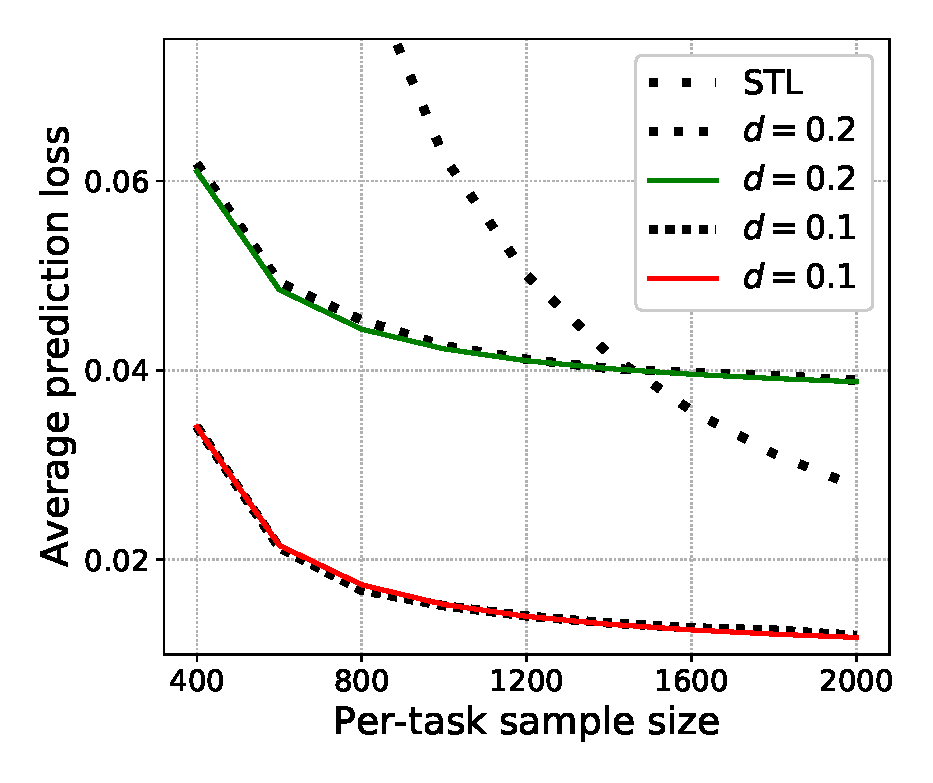
\includegraphics[width=0.35\textwidth]{figures/same_covariates.eps}
%	\caption{Validating Example \ref{ex_same_cov} in Section \ref{sec_same} for $10$ tasks: our estimated loss (solid line) matches the empirical loss (dotted line) accurately for various task-specific variance $d^2$ and sample size $n$ settings. The feature dimension $p$ is $200$, and noise variance $\sigma^2$ is $1/4$.}
%	\label{fig_same_cov}
%\end{figure}



\section{Conclusions and Discussions}\label{sec_conclude}

This work studied the generalization properties of a widely used hard parameter sharing approach for multi-task learning.
We provided sharp bias-variance tradeoffs of HPS in high-dimensional linear regression.
Using these results, we analyzed how varying sample sizes and covariate shifts impact HPS.
We rigorously explained several empirical phenomena such as negative transfer and covariate shift related to these dataset properties.
We validated our theory and conducted further studies on text classification tasks.

We describe several open questions for future work.
%First, it would be interesting to tighten our estimate in Corollary \ref{cor_MTL_loss}, which would extend the observation in Figure \ref{fig_size} to small $n_1$.
%Second, it would be interesting to extend our result to classification problems such as logistic regression.
First, our result in Corollary \ref{cor_MTL_loss} involves an error term that scales down with $n_1$.
Tightening this error bound requires showing the limit of $\normFro{({Z^{(1)}}^{\top} Z^{(1)} + {Z^{(2)}}^{\top} Z^{(2)})^{-1} {Z^{(1)}}^{\top} Z^{(1)}}^2$ for two isotropic sample covariance matrices.
This requires studying the asymptotic singular values distribution of the non-symmetric matrix $({Z^{(1)}}^{\top} Z^{(1)})^{-1}{Z^{(2)}}^{\top} Z^{(2)}+\id$, which is still an open problem in random matrix theory.
%FY: $+\id$ is very important and makes the problem very hard; otherwise the problem can be solved with current RMT methods.
The eigenvalue distribution of this matrix, which has been obtained in \citet{Fmatrix}, might help resolve this problem.
%but its singular values will follow a different distribution since the matrix is not symmetric.
 %might require new techniques beyond the current ones in random matrix theory .%\HZ{to add}.
Second, it would be interesting to extend our results to classification problems.
Several recent work has made remarkable progress for logistic regression in the high-dimensional setting (e.g. \citet{sur2019modern}).
It is an interesting question to study logistic regression in a multiple-sample setting.


\bibliographystyle{plainnat}
\balance
\bibliography{rf,ref_mtl}

\appendix
\onecolumn
\section{Further Studies on Text Classification Tasks}\label{sec_text}

Our results and their implications are all in the high-dimensional linear regression setting.
How well do they extend to other scenarios?
In this section, we conduct further studies on six text classification datasets, for predicting whether a sentence has a positive or a negative sentiment.
Our datasets include a review sentiment dataset (MR) \cite{pang2005seeing}, a sentence subjectivity dataset (SUBJ) \cite{pang2004sentimental}, a customer reviews dataset (CR) \cite{hu2004mining}, a question type dataset (TREC) \cite{li2002learning}, an opinion polarity dataset (MPQA) \cite{wiebe2005annotating}, and the Stanford sentiment treebank (SST) dataset \cite{socher2013recursive}.
%The question is to predict positive or negative sentiment expressed in the text.
Our model consists of a word embedding layer with GloVe embeddings \cite{pennington2014glove} followed by a long-short term memory (LSTM) or a multi-layer perception (MLP) layer \cite{lei2018simple}.\footnote{For MLP, we apply an average pooling layer over word embeddings. For LSTM, we add a shared feature representation layer on top of word embeddings.}

%multi-layer perceptron (MLP), LSTM, CNN on all tasks
%We use this task to verify our theoretical results on model capacity and task covariance in real world.
%{\it ChestX-ray14.} This dataset contains 112,120 frontal-view X-ray images \cite{chexnet17}.
%There are 14 diseases (tasks) for every image that we would like to predict.
%We use densenet121 as the shared module \cite{huang2017densely}.
%We treat each label as one task a binary classification problem and formulate it as a 14-task multi-task learning problem.
%This dataset is curated where the labels
%We use the CheXNet model from~\cite{chexnet}, which is a 121-layer convolutional neural network on all tasks.
%For the text classification experiment, we encode each word using the GLoVe word embeddings.%
%\footnote{http://nlp.stanford.edu/data/wordvecs/glove.6B.zip}
%We evaluate three model choices.
%\textit{Predicting transfer effect via STL results.}
%We show that the single-task based metric proposed in Section \ref{sec_similarity} can predict positive or negative transfer in MTL.
%A common challenge in the study of MTL is that the results can be hard to understand.
%It is difficult to predict when MTL performs well without running extensive trials.
%Our insight is that we can use STL results to help understand MTL results.
%Table \ref{tab:mtl_better_than_stl} shows the result on both the sentiment analysis and the ChestX-ray14 tasks.
%We find that using a threshold of $\tau = 0.1$, the STL results correctly predict positive or negative transfer with $75.6\%$ precision and $38.8\%$ recall among $30$ times $5$ (random seeds) task pairs!
%We observe similar results for $91$ task pairs from the ChestX-ray14 dataset.
%The results show that STL results are indicative of MTL results.

\paragraph{Sample size ratio.}
In Figure \ref{fig_ab_data}, we observe that for multiple example task pairs, increasing task one's sample size improves task two's prediction accuracy initially, but hurts eventually.
On the $y$-axis, we plot task two's test accuracy using HPS, subtracted by its STL test accuracy.
%validate that as we increase the sample ratio while keeping task two's sample size fixed, task two's prediction accuracy does not always increase.
We fix task one's sample size at $1000$ and increase task two's sample size from $100$ to $3000$.
These examples and the one in Figure \ref{fig_size} suggest a natural progressive training schedule, where we add samples progressively until performance drops:
%In particular, Figure \ref{fig_size} (and our analysis) shows that $L(\hat{\beta}_t^{\MTL})$ behaves as a quadratic function over $\rho_1$.
%More generally, depending on how large $\Psi(\beta_1, \beta_2)$ is, $L(\hat{\beta}_t^{\MTL})$ may also be monotonically increasing or decreasing.
%Based on this observation, we propose a progressive training schedule to improve the compuational efficiency of hard parameter sharing.
\begin{itemize}
	\item We divide the source task data into $S$ batches.
	For $S$ rounds, we incrementally add the source task data by adding one batch at a time.
	\item After training $T$ epochs, if the validation accuracy becomes worse than the previous round's result, we terminate.
%	Algorithm \ref{alg_inc_train} in Appendix \ref{app_experiments} describes the procedure in detail.
\end{itemize}
For example, if we apply this procedure to the settings of Figure \ref{fig_ab_data} and \ref{fig_size}, it will terminate until reaching the optimal sample ratio.
The advantage of this procedure is that it reduces the computational cost compared to standard round-robin training schedules.

%\begin{algorithm}[!t]
%	\caption{An incremental training schedule for efficient multi-task learning with two tasks}
%	\label{alg_inc_train}
%	\begin{algorithmic}[1]
%		\Input Two tasks $(X_1, Y_1)$ and $(X_2, Y_2)$.
%		\Param A shared module $B$, output layers $W_1, W_2$ as in the hard parameter sharing architecture.
%		\Req \# batches $S$, epochs $T$, task $2$'s validation accuracy $\hat{g}(B; W_2)$, a threshold $\tau\in(0,1)$.
%		\Output The trained modules $B, W_2$ optimized for task $2$.
%		\State Divide $(X_1, Y_1)$ randomly into $S$ batches: $(x^{(1)}, y^{(1)}), \dots, (x^{(S)}, y^{(S)})$.
%		\For{$i = 1,\dots, S$}
%			\For{$j = 1,\dots, T$}
%				\State Update $B, W_1, W_2$ using the training data $\set{x^{(k)}, x^{(k)}}_{k=1}^i$ and  $(X_2, Y_2)$.
%			\EndFor
%			\State Let $a_i = \hat{g}(B; W_2)$ be the validation accuracy.
%			\If{$a_i < a_{i-1}$ or $a_i > \tau$}
%				\State \textbf{break}
%			\EndIf
%		\EndFor
%	\end{algorithmic}
%\end{algorithm}

%We fill in the details of the experimental procedure used for the results in Figure \ref{fig_ablation}.
%\squishlist
%	\item Task similarity: We select a similar and a dissimilar source task compared to the target task using domain knowledge.
%First pair: the customer review dataset (CR) , which predicts whether a review is positive or negative, is more similar to SST (sentiment treebank) than MPQA (question type).
%Second pair: SST is more similar to MR since they both concern about positive or negative opinions expressed the text.
%TREC is less similar to MR because the task is about question types.
%Third pair: MPQA (opinion polarity) is more similar to TREC (question type)
We evaluate the progressive training procedure on the six text classification datasets.
First, we conduct multi-task training over all $15$ pairs from the six datasets.
We find that adding task one's samples progressive requires only $45\%$ of the computational cost to achieve the same test accuracy for task two than standard round-robin training schedules.
%Our insight is that since adding more samples from the source task does not always help, we can improve efficiency by adding source samples \textit{progressively} during training.
%\textbf{Improving transfer learning training efficiency.}
%We show that Algorithm \ref{alg_inc_train} also applies to transfer learning settings.
%Compared to fine-tuning the source model on the target task, we show that our proposed method reduces the computional cost by \alert{$xx\%$}, without sacrificing accuracy.
Second, we conduct multi-task training on all six datasets.
We find that adding samples progressively from all datasets requires less than $35\%$ of the computational cost to achieve the same test accuracy averaged over the six datasets than standard round-robin training schedules.
%As a further validation, excluding TREC, we observe similar comparative results.
%The data efficiency ratio of using MLP is $100\%$ because the average performance of MTL is worse than the average of STL.
%We further show that applying incremental training helps reduce the data efficiency ratio to \alert{$xx\%$}.
%If TREC is not included, we see that only $25\%$ of the labeled data is needed.



%	\begin{subfigure}[b]{0.33\textwidth}
%		\centering
%		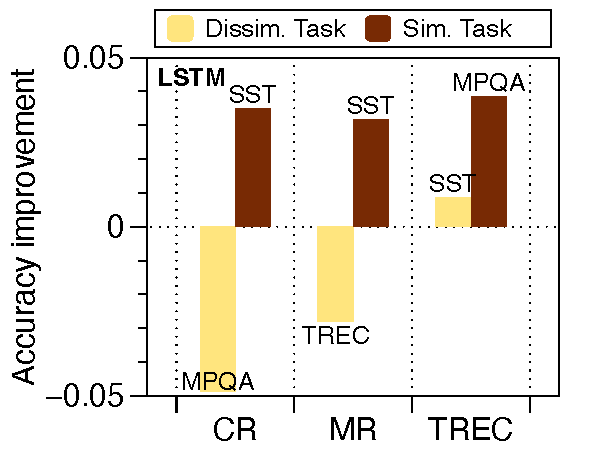
\includegraphics[width=0.975\textwidth]{figures/task_sim_norm_lstm.pdf}
%		\caption{Task similarity}
%		\label{fig_ab_sim}
%	\end{subfigure}%
%	\caption{Validating the three results of Section \ref{sec_insight} on sentiment analysis tasks. (a) Adding a semantically similar source task in MTL performs better than adding a dissimilar task.
%	(b) As source/target sample ratio increases, we observe a transition from positive to negative transfer.
%	(c)
%	Note: (S) denotes the source task and (T) denotes the target task.}


%\begin{minipage}[t]{.58\textwidth}
%	\vspace{-0.1in}
%	\centering
%  \begin{tabular}{c c c c c}
%	\toprule
%		\multirow{2}{*}{{\bf Threshold}}  & \multicolumn{2}{c}{{\bf Sentiment
%		analysis}} & \multicolumn{2}{c}{{\bf ChestX-ray14}} \\
%		& Precision &  Recall & Precision &  Recall \\
%		\cmidrule(lr){1-1} \cmidrule(lr){2-3} \cmidrule(lr){4-5}
%		0.0 & 0.596 & 1.000 & 0.593 & 1.000 \\
%		0.1 & \textbf{0.756} & \textbf{0.388} & \textbf{0.738} & \textbf{0.462} \\
%		0.2 & 0.919 & 0.065 & 0.875 & 0.044 \\
		% 0.3 & 1.000 & 0.004 &     - &     - \\
%	\bottomrule
%	\end{tabular}
%	\vspace{0.1in}
%	\captionof{table}{Single-task learning results can help predict postive or negative transfer in multi-task learning.}
%	\label{tab:mtl_better_than_stl}
%\end{minipage}%
%\quad


\paragraph{Covariate shift.}
Recall from Example \ref{ex_covshift} that having covariate shifts worsens the variance (hence the loss) of hard parameter sharing when the sample ratio increases.
This highlights the need for correcting covariate shifts when the sample ratio rises.
To this end, we study a covariance alignment procedure proposed in \citet{WZR20}, designed to correct covariate shifts.
The idea is to add an alignment module between the input and the shared module $B$.
This module is then trained together with $B$ and the output layers. We refer to \citet{WZR20} for more details about the procedure and the implementation.
%We validate our insight on this procedure in the experiments.
%We implement the covariance alignment procedure following \cite{WZR20}.

We conduct multi-task training on all $15$ task pairs from the six datasets.
In Figure \ref{fig_ab_cov}, we measure the performance gains from performing covariance alignment vs. HPS.
To get a robust comparison, we average the improvements over the 15 task pairs.
The result shows that as the sample ratio increases, performing covariance alignment provides more significant gains over HPS.
We fix task two's sample size at $1,000$, and increase task one's sample size from $1,000$ to $3,000$.

%\begin{figure}[!t]
%	\centering
%	\begin{subfigure}[b]{0.5\textwidth}
%		\centering
%		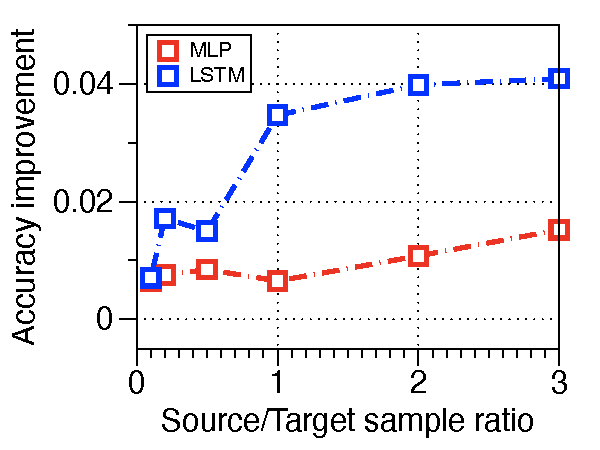
\includegraphics[width=0.5\textwidth]{figures/ratio_alignment_norm_diff_all.pdf}
%		\caption{Averaged over all 16 task pairs}
%		\label{fig_ab_cov}
%	\end{subfigure}\hfill
%	\begin{subfigure}[b]{0.5\textwidth}
%		\centering
%		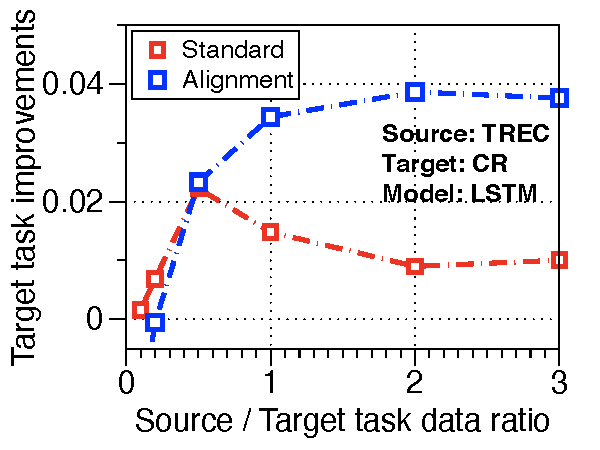
\includegraphics[width=0.5\textwidth]{figures/ratio_alignment_norm_trec_cr_lstm.pdf}
%		\caption{An example task pair}
%		\label{fig_cov_a}
%	\end{subfigure}
%	\caption{ (TREC and CR)}
%\end{figure}

%\textbf{Further results of the covariance alignment procedure.}
%Our results in Figure \ref{fig_ab_cov} are averaged over all the task pairs.
%In Figure \ref{fig_covariate_app}, we show two task pairs as examples.
%In Figure \ref{fig_cov_a}, we observe that for the particular task pair, covariance alignment provides more significant gains when the sample ratio is large.
%In Figure \ref{fig_cov_b}, we observe that covariance alignment does not always improve over the baseline multi-task learning model.
%One explanation is that MR and SST are similar tasks, hence adding the alignment module is unnecessary.
%An interesting question is to understand when adding the alignment module benefits the multi-task learning model.
%We leave this question for future work.
%Note: For text classification tasks, the source task training data size ranges from 500 to 1,500 and target task training data size is 1000; For ChestX-ray14,

%\begin{figure}[!h]
%	\centering
%	\begin{subfigure}[b]{0.48\textwidth}
%		\centering
%		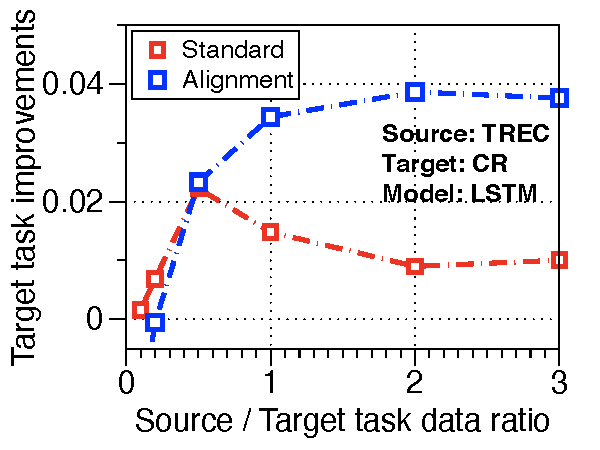
\includegraphics[width=0.7\textwidth]{figures/ratio_alignment_norm_trec_cr_lstm.pdf}
%		\caption{Task pair TREC and CR}
%		\label{fig_cov_a}
%	\end{subfigure}\hfill
%		\begin{subfigure}[b]{0.48\textwidth}
%		\centering
%		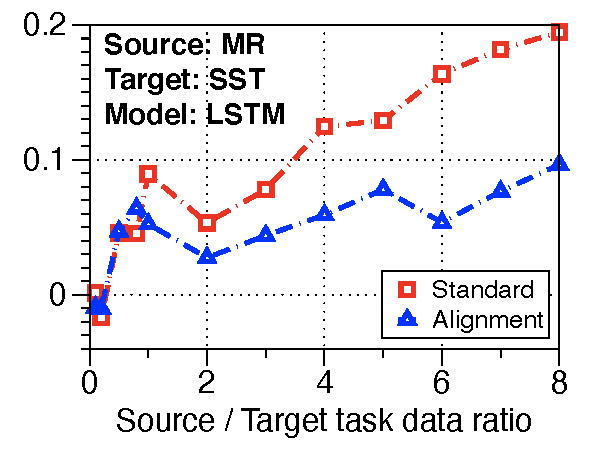
\includegraphics[width=0.7\textwidth]{figures/ratio_alignment_mr_sst_lstm.pdf}
%		\caption{Task pair MR and SST}
%			\label{fig_cov_b}
%	\end{subfigure}
%	\caption{(a) For the task pair TREC and CR, adding the covariance alignment procedure provides more improvement when the source/target sample ratio is large.
%	(b) For the task pair MR and SST, adding the covariance alignment procedure hurts performance.
%	One explanation is that MR and SST are similar tasks, hence adding the alignment module is unnecessary.}
%	\label{fig_covariate_app}
%\end{figure}


\begin{figure}%[!t]
	\begin{subfigure}[t]{0.5\textwidth}
		\centering
		\vspace{0pt}
		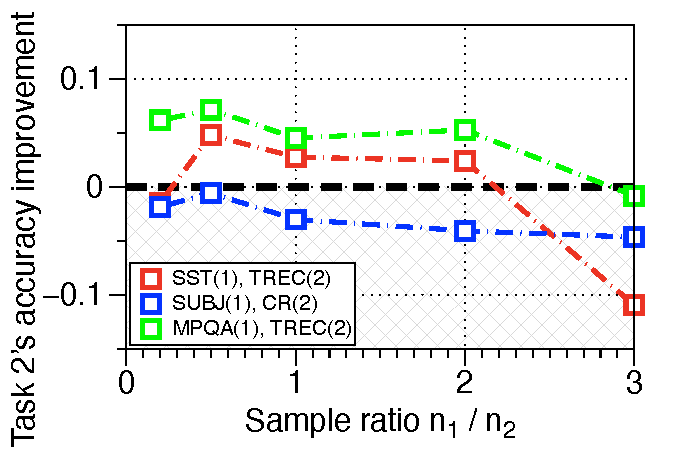
\includegraphics[width=0.8\textwidth]{figures/fig3a.pdf}
		\caption{HPS vs. STL}
		\label{fig_ab_data}
	\end{subfigure}\hfill
	\begin{subfigure}[t]{0.5\textwidth}
		\centering
		\vspace{0pt}
		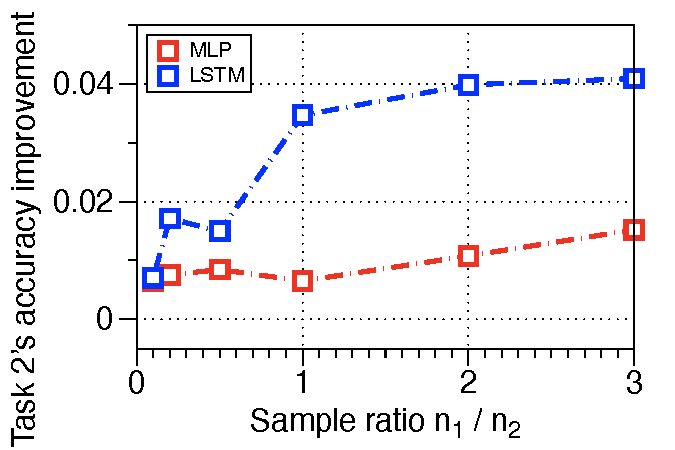
\includegraphics[width=0.8\textwidth]{figures/fig3b.pdf}
		\caption{HPS vs. covariance alignment}
		\label{fig_ab_cov}
	\end{subfigure}
	\caption{Comparing hard parameter sharing (HPS) to single-task learning (STL) and a covariance alignment approach proposed by \citet{WZR20}:
	In Figure \ref{fig_ab_data}, we observe that for multiple example task pairs, increasing task one's sample size improves task two's prediction accuracy initially, but hurts eventually -- a phenomenon similar  to Figure \ref{fig_size}.
	In Figure \ref{fig_ab_cov}, we observe that as task one's sample size increases, covariance alignment improves more over HPS.}
	\label{fig_text}
%	\begin{minipage}[t]{0.4\textwidth}
%		\centering
%		\vspace{0pt}
%		\begin{tabular}{c c c}
%		\toprule
		% \multirow{2}{*}{{\bf Models}} & \multicolumn{2}{c}{\begin{minipage}{1.2in}\begin{center}
		% Sentiment\\ analysis\end{center}\end{minipage}} \\
%		\multirow{2}{*}{{\bf Models}} & \multicolumn{2}{c}{\bf Sentiment analysis} \\
		% \cmidrule(lr){2-3}
%		& all tasks & w/o TREC \\
%		\midrule
%		{\bf MLP}  & 31\% & 29\% \\
%		{\bf LSTM} & 35\% & 34\% \\
%		{\bf CNN}  & 30\% & 28\% \\
%		\bottomrule
%		\end{tabular}
%		\captionof{table}{Finding the best sample ratio via a progressive training schedule.}
%		\label{tab:taskonomy}
%	\end{minipage}
\end{figure}


\section{Missing Proof of Theorem \ref{thm_many_tasks}}\label{app_proof_error_same_cov}

	We fill in missing details in the proof. Our first claim shows that the subspace spanned by the rows of $\hat{A}$ is close to that of $A^{\star}$.
	\begin{claim}\label{claim_opt_dist}
		Let $U_{\hat{A}} U_{\hat{A}}^{\top} \in\real^{t\times t}$ denote the subspace projection $\hat{A}^{\top} (\hat{A}\hat{A}^{\top})^{+} \hat{A}$.
		In the setting of Theorem \ref{thm_many_tasks}, we have that
		\[ \bignormFro{U_{\hat{A}} U_{\hat{A}}^{\top} - A^{\star} {A^{\star}}^{\top}}^2
				\le  n^{-c_{\varphi}} \cdot \frac{t(  \bignorm{\Sigma^{1/2} B^{\star}}^2 +  \sigma^2 )}{\lambda_r({B^{\star}}^{\top}\Sigma B^{\star})- \lambda_{r+1}({B^{\star}}^{\top}\Sigma B^{\star})}. \]
	\end{claim}
	The proof of the above claim is based on the following characterization.

	\begin{claim}\label{lem_exp_opt}
		In the setting of Theorem \ref{thm_many_tasks}, we have that
		\begin{align}
			\exarg{\set{\varepsilon^{(j)}}_{j=1}^t, X}{g(A)} = n \bignormFro{\Sigma^{1/2} B^{\star} \bigbrace{A^{\top} (AA^{\top})^{+} A - \id_{t\times t}}}^2 + \sigma^2 (n\cdot t - p \cdot r). \label{eq_gA}
		\end{align}
		As a result, the minimum of $\ex{g(A)}$, denoted by $A^{\star}{A^\star}^\top$, is the best rank-$r$ approximation of ${B^{\star}}^{\top}\Sigma B^{\star}$.
	\end{claim}

	 One can see that the expected optimization objective also admits a nice bias-variance decomposition.
	Furthermore, its minimizer only depends on the bias term since the variance term is fixed, and the minimizer of the bias term is precisely $A^{\star} {A^{\star}}^{\top}$.

	The next piece of our proof deals with the prediction loss of hard parameter sharing.
	\begin{claim}\label{claim_pred_err}
		In the setting of Theorem \ref{thm_many_tasks},
		let $\hat{a}_i = \hat{A}^{\top} (\hat{A}\hat{A}^{\top})^{+} \hat{A}_i$.
		We have that the prediction loss of $\hat{\beta}_i^{\MTL} := \hat{B} \hat{A}_i$ satisfies that
		\begin{align*}
			\bigabs{L(\hat{\beta}_i^{\MTL}) - L(B^{\star} \hat{a}_i) - \sigma^2 \norm{\hat{a}_i}^2 \cdot \bigtr{\Sigma (X^{\top}X)^{-1}}}
			\le  n^{-1/4} \left(L(B^{\star} \hat{a}_i) + \sigma^2  \cdot\|\hat a_i\|^2\right) .
		\end{align*}
	\end{claim}
	%The proof of Claim \ref{claim_opt_dist}, Claim \ref{lem_exp_opt}, and Claim \ref{claim_pred_err} can be found in Appendix \ref{app_proof_error_same_cov}.
	Provided with these results, we are ready to prove Theorem \ref{thm_many_tasks}.
	\begin{proof}[Proof of Theorem \ref{thm_many_tasks}]
		Using Claim \ref{claim_pred_err}, we get that the prediction loss of $\hat{\beta}_i^{\MTL}$ is equal to  $L(B^{\star}\hat{a}_i)+\sigma^2\norm{\hat{a}_i}^2\cdot \bigtr{\Sigma(X^{\top}X)^{-1}}$ up to a small enough error. Moreover, Claim \ref{claim_opt_dist} gives directly an upper bound on $\|\hat a_i - a_i^\star\|^2$. With this estimate, we can bound the difference
		$$L(B^{\star}\hat{a}_i)+\sigma^2\norm{\hat{a}_i}^2\cdot \bigtr{\Sigma(X^{\top}X)^{-1}} - L(B^{\star} {a}^\star_i)-\sigma^2\norm{{a}^\star_i}^2\cdot \bigtr{\Sigma(X^{\top}X)^{-1}}.$$
		Combined together, our proof is complete.
%		For the latter, we use Claim \ref{claim_opt_dist} to upper bound the difference between $\norm{\hat{a}_i}^2$ and $\norm{a_i^{\star}}^2$.
%		For $L(B^{\star}\hat{a}_i)$, we again use Claim \ref{claim_opt_dist} to upper bound the distance between $\hat{a}_i$ and $a_i^{\star}$.
%		Combined together, our proof is complete.
	\end{proof}
	
Next we present the proof of Claim \ref{claim_opt_dist}, Claim \ref{lem_exp_opt}, and Claim \ref{claim_pred_err}. 
	\begin{proof}[Proof of Claim \ref{lem_exp_opt}]
	To facilitate the analysis, we consider the following matrix notations.
	Denote
		%\[ \cE A^{\top} := {\sum_{k=1}^t \varepsilon^{(k)} A_k^{\top}}, \]
\[\cE  :=[\epsilon^{(1)},\epsilon^{(2)},\cdots, \epsilon^{(t)}],  \quad \text{ and } \quad \cW \define X(X^{\top} X)^{-1} X^{\top} \cE A^{\top} (AA^{\top})^{+}. \]
	For any $j = 1,2,\dots, t$, let
	\begin{align*}
		H_j &\define B^{\star} A^{\top} (AA^{\top})^{+} A_j - \beta^{(j)}, \quad \text{ and } \quad E_j \define \cW A_j - \varepsilon^{(j)}.
	\end{align*}
	Then we can write the function $g(A)$ conveniently as
	\[ g(A) = \sum_{j=1}^t \bignorm{X H_j + E_j}^2. \]
	We will divide $g(A)$ into three parts.
	For simplicity, we will use matrix notations in the proof, %since they are more compact.
	that is, stacking $[H_j]_j$ gives matrix $B^{\star} A^{\top} (AA^{\top}) A - B^{\star}$,
	and stacking $[E_j]_j$ gives $\cW A - \cE$.

	\paragraph{Part 1:} The first part is the square of $XH_j$,
	\begin{align}\label{eq_gA_p1}
		\sum_{j=1}^t \bignorm{X H_j}^2
		= \bignormFro{X (B^{\star} A^{\top} (AA^{\top}) A - B^{\star})}^2
		= \bignormFro{X (B^{\star} U_A U_A^{\top} - B^{\star})}^2,
	\end{align}
	where $U_{A} U_{A}^{\top} \in\real^{t\times t}$ denotes the subspace projection $ {A}^{\top} ( {A}{A}^{\top})^{+}  {A}$.
	Taking expectation of equation \eqref{eq_gA_p1} over $X$, we get
		\[ \sum_{j=1}^t \bignorm{X H_j}^2=n\bignorm{\Sigma^{1/2}(B^{\star} U_A U_A^{\top} - B^{\star})}^2. \]

	\paragraph{Part 2:} The second part is the cross term, which is equal to the following using the matrix notations:
	\begin{align}\label{eq_gA_p2}
		\sum_{j=1}^t\inner{XH_j}{E_j} = \inner{X(B^{\star} U_A U_A^{\top} - B^{\star})}{\cW A - \cE}
		= - \inner{X (B^{\star} U_A U_A^{\top} - B^{\star})}{\cE},
	\end{align}
	which is zero in expectation over $\cE$.

	\paragraph{Part 3:} The last part is the square of $E_j$:
	\begin{align}\label{eq_gA_p3}
		\sum_{j=1}^t \norm{E_j}^2 &= \bignormFro{\cW A - \cE}^2
		= \bignormFro{\cE}^2 - \inner{\cW A}{\cE},
	\end{align}
	where in the second step we use $\norm{\cW A}^2 = \inner{\cW A}{\cE}$ by algebraic calculation.
	Hence, it suffices to show that the expectation of equation \eqref{eq_gA_p3} is equal to $\sigma^2 (n\cdot t - p\cdot r)$.
	First, we have that $\ex{\|\cE\|_F^2} = \sigma^2 \cdot n \cdot t$.
%	Conditional on $X$, we have that
%	\begin{align*}
%		\exarg{\cE}{\norm{E_j}^2}
%		= \exarg{\cE}{\sum_{j=1}^t \bigbrace{\bignorm{\cW A_j}^2 - 2\inner{\cW A_j}{\varepsilon^{(j)}} }} + \sigma^2 \cdot n \cdot t.
%	\end{align*}
%	We consider both terms in the above equation one by one.
	Second, we show that
	%	\begin{align*}
	%		\inner{\cW A}{\cE} = \sigma^2 \cdot r \cdot \bigtr{U_X U_X^{\top}} = \sigma^2 \cdot r \cdot p,
	%	\end{align*}
	%because $U_X$ has rank $p$ by Fact \ref{lem_minv}.
	\begin{align*}
		\exarg{\cE}{ \inner{\cW A}{\cE}} =\exarg{\cE}{\bigtr{\cal E^\top U_X U_X^\top \cal E U_AU_A^\top} }= p\sigma^2 \cdot \bigtr{ U_AU_A^\top} =  p \sigma^2 \cdot r,
	\end{align*}
	where $U_XU_X^\top = X(X^{\top} X)^{-1} X^{\top}$.
	The first step follows by applying the definition of $\cW$.
	The last step is because $U_AU_A^\top$ has rank $r$.
	Hence, it suffices to show the second step is correct.
	For any $1\le i, j \le t$, let $\delta_{i, j} = 1$ if $i = j$, and $0$ otherwise.
	%\begin{align}
	%	\sum_{j=1}^t \norm{\cW A_j}^2 = \sum_{j=1}^t \bigtr{\cW A_j A_j^{\top} \cW^{\top}} = \bigtr{\cW AA^{\top} \cW^{\top}} = \bigtr{U_X U_X^{\top} \cE A^{\top} (AA^{\top})^{-1} A \cE^{\top}}. \label{eq_proof_same_cov_1}
	%\end{align}
	%We observe that
	Because $\varepsilon^{(i)}$ and $\varepsilon^{(j)}$ are pairwise independent, we have that
	\begin{align*}
			 \exarg{\cE}{(\cE^{\top}U_XU_X^\top \cE)_{ij} }
		&= \exarg{\cE}{{\varepsilon^{(i)}}^\top U_X U_X^\top  \varepsilon^{(j)} } = \sigma^2 \cdot \tr\left[U_XU_X^\top \right] \cdot \delta_{ij} = p\sigma^2 \cdot \delta_{ij}.
	\end{align*}
	The last step uses the fact that $\tr[U_XU_X^\top] = p$.
	Hence, the second step is correct.
	%Above, the second step used the fact that $\E(\varepsilon^{(i)}_k \varepsilon^{(i)}_l )=\sigma^2\cdot \delta_{ij}\delta_{kl}$ for $1\le k,l \le n$, and the third step used the fact that $\tr(U_XU_X^\top) =\tr(U_X^\top U_X) =p$.
	%Next, note that
	%\[ \sum_{j=1}^t \inner{\cW A_j}{\varepsilon^{(j)}} = \bigtr{\cW A\cE^{\top}}, \]
	%which is equal to equation \eqref{eq_proof_same_cov_1} by the definition of $\cW$.

	Combining the three parts, the proof is complete.
	\end{proof}
	
	\iffalse
	Second, notice that
	%\begin{align}
	%	\sum_{j=1}^t \norm{\cW A_j}^2 = \sum_{j=1}^t \bigtr{\cW A_j A_j^{\top} \cW^{\top}} = \bigtr{\cW AA^{\top} \cW^{\top}} = \bigtr{U_X U_X^{\top} \cE A^{\top} (AA^{\top})^{-1} A \cE^{\top}}. \label{eq_proof_same_cov_1}
	%\end{align}
	%We observe that
	\begin{align*}
			\exarg{\cE}{\cE A^{\top} (AA^{\top})^{+} A \cE^{\top}}
		&= \exarg{\cE}{\sum_{j=1}^t \sum_{k=1}^t \varepsilon^{(j)} A_j^{\top} (AA^{\top})^{+} A_k {\varepsilon^{(k)}}^{\top}} \\
		&= \exarg{\cE}{\sum_{j=1}^t \varepsilon^{(j)} A_j^{\top} (AA^{\top})^{+} A_j {\varepsilon^{(j)}}^{\top}} \\
		&= \sigma^2 \cdot r \cdot \id_{n\times n}.
	\end{align*}
	In the above derivation, the second step used the fact that for any $j\neq k$, $\varepsilon^{(j)}$ and $\varepsilon^{(k)}$ are pairwise independent.
	The third step used the fact that $\sum_{j=1}^t A_j^{\top} (AA^{\top})^{+} A_j = \bigtr{\id_{r\times r}} = r$, and $\ex{\varepsilon^{(j)} {\varepsilon^{(j)}}^{\top}} = \sigma^2 \cdot \id_{n\times n}$.
	Therefore, we have that
	\begin{align*}
		\exarg{\cE}{ \inner{\cW A}{\cE}} = \sigma^2 \cdot r \cdot \bigtr{X(X^{\top} X)^{-1} X^{\top}} =  \sigma^2 \cdot r \cdot \bigtr{ X^{\top}X(X^{\top} X)^{-1}}  = \sigma^2 \cdot r \cdot p.
	\end{align*}
   because $X^\top X$ is a $p\times p$ matrix.	
	%Next, note that
	%\[ \sum_{j=1}^t \inner{\cW A_j}{\varepsilon^{(j)}} = \bigtr{\cW A\cE^{\top}}, \]
	%which is equal to equation \eqref{eq_proof_same_cov_1} by the definition of $\cW$.
	Hence the proof is complete.
\fi

	\begin{proof}[Proof of Claim \ref{claim_opt_dist}]
	Corresponding to the right-hand side of \eqref{eq_gA}, we define the function
	\be\label{same_hA}h(A):= n \bignormFro{\Sigma^{1/2} B^{\star} \bigbrace{A^{\top} (AA^{\top})^{+} A - \id_{t\times t}}}^2 + \sigma^2 (n\cdot t - p \cdot r).\ee
	Let $\e$ be a fixed constant that is sufficiently small.
	Let $c_{\infty}$ be any fixed value within $(0, 1/2 - \e)$.
	To show that $U_{\hat{A}}U_{\hat{A}}^\top$ is close to $A^\star {A^\star}^\top$, we first show that $g(A)$ is close to $h(A)$ as follows:
	\begin{align}\label{eq_gA_err}
		\bigabs{g(A) - h(A)} \lesssim  n^{-c_{\varphi}} \cdot n \bignorm{\Sigma^{1/2} B^{\star} (U_AU_A^{\top} - \id_{t\times t})}_F^2 + n^{-c_{\infty}} \cdot \sigma^2 \cdot n \cdot t.
	\end{align}
%	\begin{align}\label{eq_gA_err}
%		\bigabs{g(A) - \exarg{\cE, X}{g(A)}} \lesssim p^{-c_{\varphi}} \cdot n \bignorm{\Sigma^{1/2} B^{\star} (U_AU_A^{\top} - \id)}^2 + p^{-c_{\infty}} \cdot \sigma^2 \cdot n \cdot t.
%	\end{align}
	We consider the concentration error of each part of $g(A)$.

	For equation \eqref{eq_gA_p1}, % $g_0(\cal W)= \sum_{j=1}^t\left\|Z v_j \right\|^2$.
%	$$g_0(\cal W)= \sum_{j=1}^t\left\|Z v_j \right\|^2,\quad v_j:= \Sigma^{1/2}\left(B^{\star} \cW^{\top} (\cW\cW^{\top})^{-1} W_j -  \beta_j\right).$$
%	note that $X H_j = Z \Sigma^{1/2} H_j \in \real^n$ is a random vector with i.i.d. entries of mean zero, variance $\|\Sigma^{1/2}H_j\|^2$, and finite $\varphi$-th moment by Assumption \eqref{assume_rm}.
%	Hence by the law of large numbers, we have that with high probability	
	applying Corollary \ref{cor_largedeviation} to $X H_j = Z \Sigma^{1/2} H_j$, we obtain that 
	${\left\|Z \Sigma^{1/2} H_j \right\|^2 } = { n \|\Sigma^{1/2} H_j\|^2} \cdot (1 + \OO(n^{-c_\varphi}))$ with high probability. 
	This implies that
	\begin{align}
		\abs{\sum_{j=1}^t \|X H_j\|^2 -  \sum_{j=1}^t n\norm{\Sigma^{1/2} H_j}^2} \lesssim   n^{-c_{\varphi}} \cdot n  \bignorm{\Sigma^{1/2} B^{\star} (U_{A}U_A^{\top} - \id_{t\times t})}^2. \label{eq_gA_err1}
	\end{align}

	For equation \eqref{eq_gA_p2}, 
	%using Lemma \ref{largedeviation} in Appendix \ref{app_tool} and the fact that all moments of $\varepsilon_i$ exist by Assumption \eqref{assmAhigh2}, 
	using Corollary \ref{cor_calE}, we obtain the following with high probability:
	\begin{align}
		|\inner{XB^{\star} (U_AU_A^{\top} - \id_{t\times t})}{\cE}| &\le n^\e \cdot \sigma \cdot \bignormFro{XB^{\star} (U_AU_A^{\top} - \id_{t\times t})} \nonumber \\
		&\le n^{\e} \cdot \sigma \cdot \norm{Z} \cdot \bignormFro{\Sigma^{1/2} B^{\star}(U_AU_A^{\top} -\id_{t\times t})} \nonumber \\
		&\lesssim n^{\e} \cdot \sigma \cdot \sqrt{n} \bignorm{\Sigma^{1/2} B^{\star}(U_AU_A^{\top} -\id_{t\times t})} \label{eq_gA_err2}
%		&\le  n^{c_\infty +c} \cdot \bignorm{\Sigma^{1/2} B^{\star} (U_AU_A^{\top} - \id_{t\times t})}^2 + n^{-c_{\infty}} \cdot \sigma^2 \cdot n \cdot t.
	\end{align}
	In the second step, we use the fact that $X=Z\Sigma^{1/2}$.
	In the third step, we use Fact \ref{fact_minv}(ii) to bound the operator norm of $Z$ by $\OO(\sqrt{n})$, and use $\bignormFro{\Sigma^{1/2} B^{\star}(U_AU_A^{\top} -\id_{t\times t})}\le \sqrt{t} \bignorm{\Sigma^{1/2} B^{\star}(U_AU_A^{\top} -\id_{t\times t})}$ since the matrix $\Sigma^{1/2} B^{\star}(U_AU_A^{\top} -\id_{t\times t})$ has rank at most $t$.
	By the AM-GM inequality, equation \eqref{eq_gA_err2} is bounded by the right-hand side of \eqref{eq_gA_err}.

	For equation \eqref{eq_gA_p3}, using Corollary \ref{cor_calE},
	%Lemma \ref{largedeviation} and the fact that all moments of $\varepsilon_i$ exist, 
	we obtain that with high probability,
	\begin{align}
		\abs{\normFro{\cE}^2 - \sigma^2 \cdot n \cdot t}=\abs{\tr\left[ \cal E^\top \id_{n\times n}\cal E\right] - \sigma^2 \cdot n \cdot t} &\le n^{c} \cdot \sigma^2 \| \id_{n\times n}\|_F \nonumber\\
		&= n^{1/2+c} \cdot \sigma^2 \le n^{-c_{\infty}} \cdot \sigma^2 \cdot n \cdot t. \label{eq_gA_err3}
	\end{align}
	For the inner product between $\cW A$ and $\cE$, we have that with high probability,
	\begin{align}
		\bigabs{\inner{\cW A}{\cE} - \sigma^2\cdot p \cdot r } &= \bigabs{\bigtr{\left(\cE^\top U_X U_X^{\top}\cE  - p\sigma^2 \cdot  \id_{t\times t} \right)  U_AU_A^{\top} }} \nonumber  \\
		&\le \bignormFro{U_{A} U_A^{\top}} \cdot \bignorm{\cE^\top U_X U_X^{\top} \cE - p \sigma^2 \cdot  \id_{t\times t}} \nonumber \\
		&\le \sqrt{r} \cdot n^{\e}\cdot \sigma^2\cdot \|U_X U_X^\top\|_F \nonumber \\
		&\le n^{1/2+c} \cdot \sigma^2 \cdot \sqrt{r}  \le  n^{-c_{\infty}} \cdot \sigma^2 \cdot n \cdot t.\label{eq_gA_err4}
	\end{align}
	Here in the third step, we apply equation \eqref{vcalAE3} to $\bignorm{\cE^\top U_X U_X^{\top} \cE - p \sigma^2 \cdot  \id_{t\times t}}$ and use that $ \bignormFro{U_{A} U_A^{\top}}=\sqrt{r}$ because $U_A$ has rank $r$. In the fourth step, we use $\|U_X U_X^\top\|_F=\sqrt{p}$ because $U_X$ has rank $p$.

	Combining equations \eqref{eq_gA_err1}, \eqref{eq_gA_err2}, \eqref{eq_gA_err3}, and \eqref{eq_gA_err4}, we obtain equation \eqref{eq_gA_err}.

	\bigskip
	Next, we use equation \eqref{eq_gA_err} to prove the claim.
	Using triangle inequality, we upper bound the gap between $h(A^{\star})$ and $h(\hat{A})$:  
	\begin{align}
		h(\hat{A})- h(A^{\star})   &\le \bigabs{g(A^{\star}) - h(A^{\star})} + (g(\hat A) - g({A}^{\star})) + \big|g(\hat{A}) - h(\hat{A})\big| \nonumber \\
		&\le \bigabs{g(A^{\star}) - h(A^{\star})}  + \big|g(\hat{A}) - h(\hat{A})\big|\nonumber \\
		&\lesssim n^{-c_\varphi}\cdot n \bignormFro{\Sigma^{1/2} B^{\star}}^2 + n^{-c_\infty}\cdot \sigma^2 \cdot n \cdot t. \label{eq_g_gap}
	\end{align}
	The second step used the fact that $\hat A$ is the global minimizer of $g(\cdot)$, so that $g(\hat A) \le g({A}^\star)$.
	The third step used equation \eqref{eq_gA_err} and the fact that the spectral norm of $U_A U_A^{\top} - \id_{t\times t}$ is at most one. 
	%With \eqref{eq_g_gap}, we can derive an upper bound on $\bignormFro{A^{\star} {A^{\star}}^{\top}- U_{\hat{A}} U_{\hat{A}}^{\top}}$ as follows. 
	Using equation \eqref{same_hA}, we can verify that
	$$h(\hat A)-h(A^\star) = n \bigtr{{B^\star}^\top\Sigma B^\star ( A^\star {A^\star}^\top -U_{\hat A}U^\top_{\hat A})} .$$
	Let $\lambda_1\ge\lambda_2 \ge \cdots\ge \lambda_t$ be the eigenvalues of ${B^\star}^\top\Sigma B^\star$.
	Let $v_i$ be the corresponding eigenvector of $\lambda_i$.
	Then, we have $A^\star {A^\star}^\top =\sum_{i=1}^r v_i v_i^\top$, and
	\begin{align}
	h(\hat A)-h(A^\star) = n \sum_{i=1}^r \lambda_i - n\sum_{i=1}^t \lambda_i \| U^\top_{\hat A} v_i\|^2 &= n\sum_{i=1}^r \lambda_i\left(1 -  \| U^\top_{\hat A} v_i\|^2\right)-n\sum_{i=r+1}^t \lambda_i \| U^\top_{\hat A} v_i\|^2 \nonumber\\
	&\ge  n(\lambda_r-\lambda_{r+1}) \sum_{i=r+1}^t \| U^\top_{\hat A} v_i\|^2 , \label{bdd_A-A}
	\end{align}
	where we use $\sum_{i=1}^r \left(1 -  \| U^\top_{\hat A} v_i\|^2\right) = r- \sum_{i=1}^r  \| U^\top_{\hat A} v_i\|^2 =\sum_{i=r+1}^t \| U^\top_{\hat A} v_i\|^2  $ in the last step.
	On the other hand, we have
	\begin{align*}
	\| A^\star {A^\star}^\top -U_{\hat A}U^\top_{\hat A}\|_F^2
	&= 2r - 2\inner{A^{\star}{A^{\star}}^{\top}}{U_{\hat{A}} {U_{\hat{A}}}^{\top}} \\
	&= 2 \sum_{i=r+1}^t \| U^\top_{\hat A} v_i\|^2.
	\end{align*}
	Thus from equation \eqref{eq_g_gap} and  \eqref{bdd_A-A}, we obtain that
	$$\| A^\star {A^\star}^\top -U_{\hat A}U^\top_{\hat A}\|_F^2  =2 \sum_{i=r+1}^t \| U^\top_{\hat A} v_i\|^2 \lesssim \frac{n^{-c_\varphi}\cdot  \bignormFro{\Sigma^{1/2} B^{\star}}^2 + n^{-c_\infty}\cdot \sigma^2 t}{\lambda_r- \lambda_{r+1}}  .$$
	Hence the proof is complete.
	\end{proof}
	
	\iffalse
	We simplify equation \eqref{eq_mtl_output_layer} as
	\begin{align*}
		g(A)  &= \normFro{X (X^{\top}X)^{-1} X^{\top} Y U_A U_A^{\top} - Y}^2 \\
					&= \normFro{Y}^2 - \inner{U_A U_A^{\top}}{Y^{\top} X (X^{\top} X)^{-1} X^{\top} Y}.
	\end{align*}
	We denote $H = Y^{\top} X (X^{\top} X)^{-1} X^{\top} Y$, which appears in the above equation.
	Since $\hat{A}$ is a global minimum of $g(A)$, we have that $g(A^{\star}) \ge g(\hat{A})$.
	Hence, we have
	\begin{align}
		g(A^{\star}) - g(\hat{A}) &= \abs{g(A^{\star}) - g(\hat{A})} = \abs{\inner{H}{A^{\star} {A^{\star}}^{\top} - U_{\hat{A}} U_{\hat{A}}^{\top}}} \nonumber \\
												&\ge \lambda_{\min}(H) \cdot \normFro{A^{\star} {A^{\star}}^{\top} - U_{\hat{A}} U_{\hat{A}}^{\top}}. \label{eq_g_gap1}
	\end{align}
	Recall that $Y = X B^{\star} + \cE$ in matrix notation.
	We bound the minimum singular value of $H$ as follows
	\begin{align}
		\lambda_{\min}(H) &= \lambda_{\min}({B^{\star}}^{\top} X^{\top} X B^{\star} + \cE^{\top} X (X^{\top} X)^{-1} X^{\top} \cE) \nonumber \\
		&\ge \lambda_{\min}({B^{\star}}^{\top}X^{\top}X B^{\star}) + \lambda_{\min}(\cE^{\top} X (X^{\top} X)^{-1} X^{\top} \cE) \nonumber \\
		&\ge \lambda_{\min}({B^{\star}}^{\top}\Sigma B^{\star}) \cdot \lambda_{\min}(Z^{\top}Z) + \lambda_{\min}(\cE^{\top} X (X^{\top} X)^{-1} X^{\top} \cE) \nonumber \\
		&\ge \lambda_{\min}({B^{\star}}^{\top}\Sigma B^{\star}) \cdot ((\sqrt n - \sqrt p)^2 - n \cdot p^{-c}) + \sigma^2 \cdot p \cdot (1 - p^{-1/2 + \e}). \label{eq_g_gap2}
	\end{align}
	The second equation uses the fact that the minimum singular value of the sum of two PSD matrices is greater than the sum of the minimum singular value of each matrix.
	The third equation uses the fact that $X = Z \Sigma^{1/2}$ and Fact \ref{fact_proof_gA} in Appendix \ref{app_tool}.
	The last equation uses Fact \ref{fact_minv} (ii) for the minimum singular value of $Z^{\top}Z$ and Lemma \ref{largedeviation} for $\cE\cE^{\top}$.

	Combining equation \eqref{eq_g_gap}, \eqref{eq_g_gap1}, and \eqref{eq_g_gap2}, we conclude that
	\begin{align*}
		\bignormFro{A^{\star} {A^{\star}}^{\top}- U_{\hat{A}} U_{\hat{A}}^{\top}}
		&\le \frac{p^{-c} \cdot n \bignormFro{\Sigma^{1/2} B^{\star}}^2 + p^{-1/2 + c} \cdot \sigma^2 nt} {\lambda_{\min}(H)} \\
		&\le \frac{p^{-c} \rho \normFro{\Sigma^{1/2} B^{\star}}^2 + p^{-1/2 + \e} \cdot \sigma^2 \rho t}{\lambda_{\min}^2(\Sigma^{1/2} B^{\star}) ((\sqrt{\rho} - 1)^2 - \rho \cdot p^{-c}) + \sigma^2 (1 - p^{-1/2 + \e})}
	\end{align*}
	Hence for large enough $p$, we obtain that Claim \ref{claim_opt_dist} holds.
	\fi
	

	\begin{proof}[Proof of Claim \ref{claim_pred_err}]
	%We apply similar arguments from Claim \ref{lem_exp_opt} and \ref{claim_opt_dist} for this proof.
	The proof is similar to that of equation \eqref{eq_gA_err}.
	The prediction loss of hard parameter sharing for task $i$ is equal to
	\begin{align*}
		L(\hat{\beta}_i^{\MTL}) &= \bignorm{\Sigma^{1/2} (\hat{B} \hat{A}_i - \beta^{(i)})}^2 \\
		&= \bignorm{\Sigma^{1/2} ((X^{\top} X)^{-1} X^{\top} Y \hat{A}^{\top} (\hat{A} \hat{A}^{\top})^{+} \hat{A}_i - \beta^{(i)})}^2 \\
		&= \bignorm{\Sigma^{1/2} (B^{\star} \hat{a}_i - \beta^{(i)} + R_i)}^2,
	\end{align*}
	where we denote $R_i = (X^{\top} X)^{-1} X^{\top} \cE \hat{a}_i$.
	We divide the prediction loss into three parts.

	\paragraph{Part 1:} The first part is the bias term:
	$\norm{\Sigma^{1/2} (B^{\star} \hat{a}_i - \beta^{(i)})}^2 = L(B^{\star} \hat{a}_i)$.

	\paragraph{Part 2:} The second part is the cross term, whose expectation over $\cE$ is zero.
	Let $b = B^{\star} \hat{a}_i - \beta^{(i)}$ for simplicity.
	Using Corollary \ref{cor_calE}, the concentration error can be bounded as
	\begin{align*}
		\bigabs{\inner{\Sigma^{1/2}b}{\Sigma^{1/2}R_i}}
		&= \bigabs{\inner{X (X^{\top}X)^{-1} \Sigma b \hat{a}_i^{\top}}{\cE}} \\
		&\le \sum_{j=1}^t \abs{\hat{a}_i(j)} \cdot \bigabs{\inner{X (X^{\top} X)^{-1} \Sigma b}{\varepsilon^{(j)}}} \\
		&\le \sum_{j=1}^t \abs{\hat{a}_i(j)} \cdot n^{\e}\sigma \bignorm{X (X^{\top}X)^{-1} \Sigma b} \\
		&\le \sqrt{t} \norm{\hat{a}_i} \cdot n^{\e} \sigma \bignormFro{X (X^{\top} X)^{-1} \Sigma b}.
	\end{align*}
%	\begin{align*}
%		\bigabs{\inner{\Sigma^{1/2}(B^{\star} \hat{a}_i - \beta_i)}{\Sigma^{1/2}R_i}} &= \bigabs{\inner{\hat a_i^\top X(X^\top X)^{-1}\Sigma (B^{\star} \hat{a}_i - \beta_i)}{\cal E}} \\
%		&\le n^{c}\sigma \cdot \bignormFro{\hat a_i^\top X(X^\top X)^{-1}\Sigma (B^{\star} \hat{a}_i - \beta_i)}\\
%		&\le n^{c}\sigma \cdot\|\hat a_i\| \cdot  \|\Sigma^{1/2}(B^{\star} \hat{a}_i - \beta_i)\| \cdot \| (Z^\top Z)^{-1} \|^{1/2} \\
%		&\lesssim n^{-1/2+c}\sigma \cdot\|\hat a_i\| \cdot \bignorm{\Sigma^{1/2}(B^{\star} \hat{a}_i - \beta_i)} \\
%		&\le n^{-1/2+c}\sigma^2  \cdot\|\hat a_i\|^2 + n^{-1/2+c} L(B^{\star} \hat{a}_i), 
%	\end{align*}
	In the first step, we plug in the definition of $R_i$ and re-arrange terms.
	In the second step, we use $\hat{a}_i(j)$ to denote the $j$-th coordinate of $\hat{a}_i$.
	In the third step, we use equation \eqref{vcalE}.
	In the last step, we use $\sum_j |\hat a_i(j)|\le \sqrt{t}\|\hat a_i\|$ by Cauchy-Schwarz inequality.
	Finally, we have
	\begin{align*}
		\bignormFro{ X(X^\top X)^{-1}\Sigma b} &=\left[ {b}^\top \Sigma (X^\top X)^{-1}X^\top X(X^\top X)^{-1}\Sigma b \right]^{1/2} \\
		&\le  \|\Sigma^{1/2} b \|  \cdot \left\| \Sigma^{1/2}(X^\top X)^{-1}\Sigma ^{1/2} \right\|^{1/2}  =   \|\Sigma^{1/2} b \|  \cdot \left\| (Z^\top Z)^{-1}\right\|^{1/2} \\
		&\le n^{-1/2} \cdot \norm{\Sigma^{1/2} b}.
	\end{align*}
%	\begin{align*}
%	\bignormFro{\hat a_i^\top X(X^\top X)^{-1}\Sigma (B^{\star} \hat{a}_i - \beta_i)} &=\|\hat a_i\|\cdot \left[ (B^{\star} \hat{a}_i - \beta_i)^\top \Sigma (X^\top X)^{-1}X^\top X(X^\top X)^{-1}\Sigma (B^{\star} \hat{a}_i - \beta_i) \right]^{1/2} \\
%	&\le \|\hat a_i\|\cdot  \|\Sigma^{1/2}(B^{\star} \hat{a}_i - \beta_i)\|  \cdot \left\| \Sigma^{1/2}(X^\top X)^{-1}\Sigma ^{1/2} \right\|^{1/2} \\
%	&= \|\hat a_i\|\cdot  \|\Sigma^{1/2}(B^{\star} \hat{a}_i - \beta_i)\|  \cdot \left\| (Z^\top Z)^{-1}\right\|^{1/2}
%	\end{align*}
	Above, we use $X=Z\Sigma^{1/2}$. In the last step, we use Fact \ref{fact_minv}(ii) to bound the operator norm of $Z^\top Z$ by $\OO(n^{-1})$. %, and apply the AM-GM inequality.
	One can see that the concentration error from this part is upper bounded by the result in Claim \ref{claim_pred_err}.
	
	\iffalse
	Next, we use the fact that the spectral norm of $\cE$ is at most $\sigma \cdot p^{\e}$.
	Hence, the spectral norm of $\Sigma^{1/2} E_i$ is at most
		\[ \sigma \cdot p^{\e} \cdot \norm{\Sigma^{1/2} (X^{\top} X)^{-1} X^{\top}} \cdot \norm{\hat{a}_i}. \]
	Therefore, the cross term is bounded by $\sigma \cdot p^{\e}$ times
	\begin{align*}
			& \bignorm{\Sigma^{1/2} (B^{\star} \hat{a}_i - \beta_i)} \cdot \norm{\Sigma^{1/2} (X^{\top} X)^{-1} X^{\top}} \cdot \norm{\hat{a}_i} \\
		\le & \bignorm{\Sigma^{1/2} (B^{\star} \hat{a}_i - \beta_i)}^2 + \norm{\hat{a}_i}^2 \cdot \bignorm{\Sigma^{1/2} (X^{\top} X)^{-1} X^{\top}}^2 \tag{by Cauchy-Shwartz inequality} \\
		\le & \bignorm{\Sigma^{1/2}(B^{\star} \hat{a}_i - \beta_i)} + \norm{\hat{a}_i}^2 \cdot \bigtr{\Sigma (X^{\top} X)^{-1}}.
	\end{align*}
	\fi

	\paragraph{Part 3:} The final part is the squared term of $R_i$. We rewrite it as
	\begin{align}
	\|\Sigma^{1/2}R_i\|^2 &= \left\|\sum_{j=1}^t \hat{a}_i(j) \Sigma^{1/2}(X^{\top} X)^{-1} X^{\top} \epsilon^{(j)}\right\|^2 \nonumber\\
	& = \sum_{1\le j , k \le t}\hat a_i(j) \hat a_i(k)  {\epsilon^{(j)}}^\top X(X^{\top} X)^{-1}\Sigma (X^{\top} X)^{-1} X^{\top} {\epsilon^{(k)}}.\label{E_i^2}
	\end{align}	
%	If $j\ne k$, using Corollary \ref{cor_calE} we obtain that 
%	\begin{align}
%	\left|{\epsilon^{(j)}}^\top X(X^{\top} X)^{-1}\Sigma (X^{\top} X)^{-1} X^{\top} {\epsilon^{(k)}} \right| &\le \sigma^2 \cdot \bignormFro{X(X^{\top} X)^{-1}\Sigma (X^{\top} X)^{-1} X^{\top} } \nonumber\\
%	& =\sigma^2 \cdot \bignormFro{\Sigma^{1/2}(X^{\top} X)^{-1}\Sigma^{1/2}} \nonumber\\
%	&  \le \sigma^2 \cdot p^{1/2} \cdot \bignorm{(Z^{\top} Z)^{-1}} \lesssim \sigma^2 \cdot n^{-1/2+c} \label{jnek}
%	\end{align}
%	with high probability for any small constant $c>0$. On the other hand, if $j=k$, 
	First, for any $1 \le j, k \le t$, the expectation is
	$$\exarg{\cal E}{{\epsilon^{(j)}}^\top X(X^{\top} X)^{-1}\Sigma (X^{\top} X)^{-1} X^{\top} \epsilon^{(k)}}=\delta_{jk}\cdot \sigma^2\tr\left[\Sigma(X^\top X)^{-1}\right] .$$
	Second, using equation \eqref{vcalA2}, the concentration error is at most
	\begin{align}
	& \left|{\epsilon^{(j)}}^\top X(X^{\top} X)^{-1}\Sigma (X^{\top} X)^{-1} X^{\top} {\epsilon^{(k)}} -\delta_{jk}\cdot \sigma^2\tr\left[\Sigma(X^\top X)^{-1}\right]\right|\nonumber \\
	\le &n^c\cdot \sigma^2  \bignormFro{X(X^{\top} X)^{-1}\Sigma (X^{\top} X)^{-1} X^{\top} }   = n^c\cdot \sigma^2  \bignormFro{\Sigma^{1/2}(X^{\top} X)^{-1}\Sigma^{1/2}} \nonumber\\
	  \le &\sigma^2 \cdot p^{1/2} \cdot  \bignorm{(Z^{\top} Z)^{-1}}^{1/2} \lesssim \sigma^2 \cdot n^{-1/2+c}. \label{jeqk}
	\end{align}
	Above, we used Fact \ref{fact_minv}(ii) in the last step to bound the operator norm of $(Z^{\top} Z)^{-1}$.
	Plugging equation \eqref{jeqk} into equation \eqref{E_i^2}, we obtain that 
	\begin{align*}
		\bigabs{\bignorm{\Sigma^{1/2} R_i}^2 -  \sigma^2 \|\hat a_i\|^2 \cdot\tr\left[\Sigma(X^\top X)^{-1}\right]} \lesssim  \sigma^2 \cdot n^{-1/2+c}  \sum_{1\le j,k\le t}|\hat a_i(j)||\hat a_i(k)| =  n^{-1/2+c} \sigma^2 \cdot  \|\hat a_i\|^2.
	\end{align*}
%	One can verify that the expectation of $\norm{\Sigma^{1/2} E_i}^2$ is equal to $\sigma^2 \norm{\hat{a}_i}^2 \cdot \tr[\Sigma (X^{\top} X)^{-1}]$.
%	Next, we bound the concentration error.
%	Let $A = X (X^{\top} X)^{-1} \Sigma (X^{\top} X)^{-1} X^{\top}$.
%	We have that
%	\begin{align*}
%		\bigabs{\bignorm{\Sigma^{1/2} E_i}^2 - \exarg{\cE}{\bignorm{\Sigma^{1/2} E_i}^2}}
%		&= \bigabs{\inner{A}{\cE \hat{a}_i \hat{a}_i^{\top} \cE^{\top} - \exarg{\cE}{\cE \hat{a}_i \hat{a}_i^{\top} \cE}}}.
%	\end{align*}
%	In the above equation, we note that the trace of $A$ is precisely the trace of $\Sigma (X^{\top} X)^{-1}$.
%	On the other hand, the concentration error of the spectral norm of $\cE \hat{a}_i \hat{a}_i^{\top} \cE^{\top}$ is at most $\sigma^2 \e $.

	Finally, combining the three parts together, we complete the proof.
\end{proof}

\section{Proof of Theorem \ref{thm_main_RMT}}\label{appendix RMT}
We first state the bias limit for the term in equation \eqref{eq_bias_2task}.

\begin{theorem}\label{thm_main_RMT_app}
	In the setting of Theorem \ref{thm_main_RMT}, the bias equation \eqref{eq_bias_2task} satisfies the following limit with high probability for any fixed unit vector $w\in\real^p$:
			\begin{align}\label{lem_cov_derv_eq}
				\bigabs{w^{\top} \Sigma^{(1)} \bigbrace{\hat{\Sigma}^{-1} \Sigma^{(2)} \hat{\Sigma}^{-1} - \frac{1}{(n_1+n_2)^2}{\Sigma^{(2)}}^{-1/2} V {\frac{a_3 \Lambda^2 + (a_4 + 1)\id}{(a_1 \Lambda^2 + a_2\id)^2}} V^{\top} {\Sigma^{(2)}}^{-1/2}} \Sigma^{(1)} w} \le  \frac{p^{-c_{\varphi}}}{(n_1+n_2)^2},
			\end{align}
				where $a_{3}$ and $a_4$ are the solutions of the following self-consistent equations % with $b_k = \frac1{p}\sum_{i=1}^p \frac{\lambda_i^{2k}} {(\lambda_i^2 a_1 + a_2)^2}$, for $k = 0, 1, 2$:
			\begin{align}\label{eq_a34extra}
				a_3 + a_4 = \frac{1}{n_1 + n_2}\sum_{i=1}^p \frac{1}{\lambda_i^2 a_1 + a_2}, \ \
				a_3 + \frac{1}{n_1 + n_2} \sum_{i=1}^p \frac{\lambda_i^2 (a_2 a_3-a_1 a_4 )}{(\lambda_i^2 a_1 + a_2)^2} = \frac{1}{n_1 + n_2} \sum_{i=1}^p \frac{\lambda_i^2 a_1}{(\lambda_i^2 a_1 + a_2)^{2}}.
%				\left(\frac{\rho_1}{a_1^{2}} -  b_2  \right)\cdot  a_3 -  b_1 \cdot  a_4 = b_1,\quad \left(\frac{\rho_2}{a_2^{2}}-  b_0\right)\cdot  a_4 - b_1 \cdot  a_3
%				= b_0.
			\end{align}
\end{theorem}
In this section, we give the proof of Theorem \ref{thm_main_RMT} and Theorem \ref{thm_main_RMT_app}

\subsection{Proof Overview}
Since the full proof of Theorem \ref{thm_main_RMT} and Theorem \ref{thm_main_RMT_app} is rather technical, in this subsection we give a more detailed proof overview, which contains the main ideas of the proof. 

Recall that $(W-z\id)^{-1}$ is the resolvent of matrix $W$. 
We say that $(W-z\id)^{-1}$ converges to a deterministic $p\times p$ matrix limit $R(z)$ if for any sequence of deterministic unit vectors $v\in \R^p$,
$$v^\top \left[(W-z\id)^{-1}-R(z)\right]v\to 0\ \ \ \text{when $p$ goes to infinity.
}$$

To study $W$'s resolvent, we observe that $W$ is equal to $\AF\AF^{\top}$ for a $p$ by $n_1 + n_2$ matrix
	\be\label{defn AF} \AF := (n_1+ n_2)^{-1/2} [\Lambda U^\top (Z^{(1)})^\top,V^\top (Z^{(2)})^\top]. \ee
%}\HZ{what does this trick mean? use less technical words},
%This idea dates back at least to Girko, see e.g., the works \cite{girko1975random,girko1985spectral} and references therein.
Consider the following symmetric block matrix whose dimension is $p + n_1 + n_2$
%which is a linear function of $(Z^{(1)})$ and $(Z^{(2)})$:
%\begin{definition}[Linearizing block matrix]\label{def_linearHG}%definiton of the Green function
%We define the $(n+N)\times (n+N)$ block matrix
 \begin{equation}\label{linearize_block}
    H \define \left( {\begin{array}{*{20}c}
   0 & \AF  \\
   \AF^{\top} & 0
%   {Z^{(2)}V} & 0 & 0
   \end{array}} \right).
 \end{equation}
For this block matrix, we define its resolvent as
$$G(z) \define \left[H - \begin{pmatrix}z\id_{p\times p}&0\\ 0 & \id_{(n_1+n_2)\times (n_1+n_2)} \end{pmatrix}\right]^{-1},$$
%as the resolvent of $H$,
for any complex value $z\in \mathbb C$.
Using Schur complement formula for the inverse of a block matrix, it is not hard to verify that
	\begin{equation} \label{green2}
	  G(z) =  \left( {\begin{array}{*{20}c}
			(W- z\id)^{-1} & (W - z\id)^{-1} \AF  \\
      \AF^\top (W - z\id)^{-1} & z(\AF^\top \AF - z\id)^{-1}
		\end{array}} \right).%\quad \cal G_R:=(W^\top W - z)^{-1} ,
  \end{equation}



\paragraph{Variance asymptotic limit.}
In Theorem \ref{main_cor}, we will show that for $z$ in a small neighborhood around $0$, when $p$ goes to infinity, $G(z)$ converges to the following limit
\be \label{defn_piw}
	\Gi(z) \define \begin{pmatrix} (a_{1}(z)\Lambda^2  +  (a_{2}(z)- z)\id_{p\times p})^{-1} & 0 & 0 \\ 0 & - \frac{n_1+n_2}{n_1} a_{1}(z)\id_{n_1\times n_1} & 0 \\ 0 & 0 & -\frac{n_1+n_2}{n_2}a_{2}(z)\id_{n_2\times n_2}  \end{pmatrix},\ee
where $a_1(z)$ and $a_2(z)$ are the unique solutions to the following self-consistent equations
\be\label{selfomega_a}
\begin{split}
	&a_1(z) + a_2(z) = 1 - \frac{1}{n_1 + n_2} \bigbrace{\sum_{i=1}^p \frac{\lambda_i^2 a_1(z) + a_2(z)}{\lambda_i^2 a_1(z) + a_2(z) - z}}, \\ %\label{selfomega_a000} \\
	&a_1(z) + \frac{1}{n_1 + n_2}\bigbrace{\sum_{i=1}^p \frac{\lambda_i^2 a_1(z)}{\lambda_i^2 a_1(z) + a_2(z) - z}} = \frac{n_1}{n_1 + n_2}.
% \frac{\rho_1}{a_{1}(z)} = \frac{1}{p}\sum_{i=1}^p \frac{\lambda_i^2}{ - z+\lambda_i^2 a_{1}(z) +a_{2} (z) } + (\rho_1+\rho_2),\  \frac{\rho_2}{a_{2}(z)} = \frac{1}{p}\sum_{i=1}^p \frac{1 }{  -z+\lambda_i^2 a_{1}(z) +  a_{2}(z)  }+ (\rho_1+\rho_2) .
\end{split}
\ee
The existence and uniqueness of solutions to the above system are shown in Lemma \ref{lem_mbehaviorw}.
%First, we define the deterministic limits of $(m_1(z), m_{2}(z))$ by $\left(-\frac{\rho_1+\rho_2}{\rho_1}a_{1}(z),-\frac{\rho_1+\rho_2}{\rho_2}a_{2}(z)\right)$, where
%satisfying that $\im a_{1}(z)< 0$ and $\im a_{2}(z)<0$ for $z\in \C_+$ with $\im z$.
%\be\label{ratios}
% \gamma_n :=\frac{p}{n}=\frac{1}{\rho_1+\rho_2},\quad r_1 :=\frac{n_1}{n}=\frac{\rho_1}{\rho_1+\rho_2},\quad r_2 :=\frac{n_2}{n}=\frac{\rho_2}{\rho_1+\rho_2}.
%\ee
Given this result, we now show that when $z = 0$, the matrix limit $\Gi(0)$ implies the variance limit shown in equation \eqref{lem_cov_shift_eq}.
First, we have that $a_1 = a_1(0)$ and $a_2 = a_2(0)$ since the equations in \eqref{selfomega_a} reduce to equations \eqref{eq_a12extra000} and \eqref{eq_a12extra} when $z=0$.
Second, since $W^{-1}$ is the upper-left block matrix of $G(0)$, we have that $W^{-1}$ converges to $ (a_1\Lambda^2 + a_2\id)^{-1} $.
Using the fact that $\tr[\Sigma^{(2)} \hat{\Sigma}^{-1}] = (n_1 + n_2)^{-1}\bigtr{W^{-1}} $, we get that when $p$ goes to infinity, % the trace of $$ converges to
\begin{align*}
  \bigtr{\Sigma^{(2)} \hat{\Sigma}} \rightarrow \frac{1}{n_1+n_2}\bigtr{(a_1 \Lambda^2 + a_2\id)^{-1}} &= \frac1{n_1+n_2}\bigtr{(a_1 M^{\top}M + a_2 \id)^{-1}} \\
  &=\frac{1}{n_1+n_2} \bigtr{\Sigma^{(2)} (a_1 \Sigma^{(1)} + a_2 \Sigma^{(2)})^{-1}},
  \end{align*}
%\noindent{\bf Variance asymptotics.} Using definition \eqref{mainG}, we can write equation \eqref{eigen2extra} as
%\be\label{rewrite X as R} [(X^{(1)})^\top X^{(1)}+(X^{(2)})^\top X^{(2)}]^{-1}=n^{-1}\Sigma_2^{-1/2}V\cal G(0)V^\top\Sigma_2^{-1/2}.\ee
%When $z=0$, it is easy to check that , which means that we actually have $a_1(0)=a_1$ and $a_2(0)=a_2$. Hence the matrix limit of $\cal G(0)$ is given by $(a_{1}\Lambda^2 + a_{2}\id_p)^{-1}$. Then inserting this limit into equation \eqref{rewrite X as R}, we can write the left-hand side of equation \eqref{lem_cov_shift_eq} as
%\begin{align}
%&\bigtr{\left( (X^{(1)})^{\top}X^{(1)} + (X^{(2)})^{\top}X^{(2)}\right)^{-1} \Sigma}\approx n^{-1}\bigtr{\Sigma_2^{-1/2}V\cal (a_{1}\Lambda^2 + a_{2}\id_p)^{-1}V^\top\Sigma_2^{-1/2}\Sigma}  \nonumber\\
%&=n^{-1}\bigtr{\Sigma_2^{-1/2}\cal (a_{1}\Sigma_2^{-1/2}\Sigma_1\Sigma_2^{-1/2} + a_{2}\id_p)^{-1}\Sigma_2^{-1/2}\Sigma}  = n^{-1}\bigtr{\cal (a_{1} \Sigma_1  + a_{2}\Sigma_2)^{-1}\Sigma}  ,\label{Gi00}
%\end{align}
where we note that $M^\top M = (\Sigma^{(2)})^{-1/2} \Sigma^{(1)} (\Sigma^{(2)})^{-1/2}$ and its SVD is equal to $V^{\top}\Lambda^2 V$.
%For the asymptotic limit, its concentration error is shown in Appendix \ref{appendix RMT}.




\paragraph{Bias asymptotic limit.}
 For the bias limit in equation \eqref{lem_cov_derv_eq}, we show that it is governed by the derivative of $(W - z\id)^2$ with respect to $z$ at $z = 0$.
First, we can express the empirical bias term in equation \eqref{lem_cov_derv_eq} as %$W$
\begin{align}\label{calculate G'}
	(n_1 + n_2)^2 \hat{\Sigma}^{-1}\Sigma^{(2)}\hat{\Sigma}^{-1} = {\Sigma^{(2)}}^{-1/2} V W^{-2} V^{\top} {\Sigma^{(2)}}^{-1/2}.
\end{align}
Let $\cal G(z):=(W-z\id )^{-1}$ denote the resolvent of $W$.
Our key observation is that $\frac{\dd{\cal G(z)}}{\dd z} =  \cal G^2(z)$.
Hence, provided that the limit of $(W - z\id)^{-1}$ is $(a_1(z) \Lambda^2 + (a_2(z) - z) \id)^{-1}$ near $z = 0$, the limit of $\frac{\dd{\cal G(0)}}{\dd z}$ satisfies that
\begin{align}\label{cal G'0}
	\frac{\dd \cal G(0)}{\dd z} \to \frac{-\frac{\dd a_1(0)}{\dd z}\Lambda^2 - (\frac{\dd a_2(0)}{\dd z} - 1)\id}{(a_{1}(0)\Lambda^2 + a_{2}(0)\id_p)^2}.
\end{align}
To find the derivatives of $a_1(z)$ and $a_2(z)$, we take the derivatives on both sides of the system of equations \eqref{selfomega_a}.
%\begin{align*}
%	\frac{\dd a_1(z)}{\dd z} + \frac{\dd a_2(z)}{\dd z} = -\frac{1}{n_1 + n_2} \sum_{i=1}^p \frac{1}{\lambda_i^2 a_1 + a_2},
%	\frac{\dd a_1(z)}{\dd z} + \frac{1}{n_1 + n_2}\sum_{i=1}^p \frac{\lambda_i^2 (a_1'(z) a_2 - a_2'(z) a_1)}{(\lambda_i^2 a_1 + a_2)^2} = -\frac{1}{n_1 + n_2} \sum_{i=1}^p \frac{\lambda_i^2 a_1}{(\lambda_i^2 a_1 + a_2)^2}
%\end{align*}
Let $a_3 = - \frac{\dd a_1(0)}{\dd z}$ and $a_4 = - \frac{\dd a_2(0)}{\dd z}$.
%then taking implicit differentiation of equation \eqref{selfomega_a}
One can verify that $a_3$ and $a_4$ satisfy the self-consistent equations in \eqref{eq_a34extra} (details omitted).
Applying equation \eqref{cal G'0} to equation \eqref{calculate G'}, we obtain the asymptotic limit of the bias term.
%\begin{align}
%& n^2\bignorm{\Sigma_2^{1/2} \bigbrace{ (X^{(1)})^{\top}(X^{(1)}) + (X^{(2)})^{\top}(X^{(2)}) }^{-1} \Sigma_1^{1/2} w}^2 \nonumber\\
%&\approx  w^\top \Sigma_1^{1/2}\Sigma_2^{-1/2}V\frac{a_3\Lambda^2 +(1+ a_4)\id_p}{(a_{1}\Lambda^2 + a_{2}\id)^2}V^\top \Sigma_2^{-1/2}\Sigma_1^{1/2}w= w^{\top} \Pi_\bias w, \label{calculatePibias}
%\end{align}
%where in the last step we used $M = \Sigma_1^{1/2}\Sigma_2^{-1/2}$ and $V \Lambda^2 V^\top=M^\top M$. This concludes equation \eqref{lem_cov_derv_eq}.

As a remark, in order for $\frac{\dd \cal G(z)}{\dd z}$ to stay close to its limit at $z = 0$, we not only need to find the limit of $\cal G(0)$, but also the limit of $\cal G(z)$ within a small neighborhood of $0$.
This is why we consider $W$'s resolvent for a general $z$. %as opposed to the Stieljes transform of its empirical spectral distribution.

\paragraph{Schur complement and self-consistent equations.}
We briefly describe how to derive the matrix limit $\Gi(z)$.
First, we consider the special case where $Z^{(1)}$ and $Z^{(2)}$ are both multivariate Gaussian random matrices.
By rotational invariance, we have that $Z^{(1)} U$ and $Z^{(2)} V$ are still multivariate Gaussian random matrices.
Next, we use the Schur complement formula to deal with the resolvent $G(z)$.
We show that $G(z)$'s diagonal entries satisfy a set of self-consistent equations in the limit, leading to equations in \eqref{selfomega_a}.
On the other hand, $G(z)$'s off-diagonal entries are approximately zero using standard concentration bounds.
Finally, we extend our result to general random matrices under the finite $\varphi$-th moment condition.
We prove an anisotropic local law using recent developments in random matrix theory \cite{erdos2017dynamical,Anisotropic}.
A complete proof of Theorem \ref{thm_main_RMT} will be given in Appendix \ref{sec pf RMTlemma}-Appendix \ref{sec entry}. %Appendix \ref{appendix RMT}.













We begin with a warm up analysis when the entries of $Z^{(1)}$ and $Z^{(2)}$ are drawn i.i.d. from an isotropic Gaussian distribution. 
By the rotational invariance of the multivariate Gaussian distribution, we have that the entries of $Z^{(1)} U$ and $Z^{(2)}V$ also follow an isotropic Gaussian distribution.
Hence it suffices to consider the following resolvent
 \begin{equation} \label{resolv Gauss1}
   G(z)= \left( {\begin{array}{*{20}c}
   { -z\id_{p\times p} } & (n_1+n_2)^{-1/2}\Lambda (Z^{(1)})^\top & (n_1+n_2)^{-1/2} (Z^{(2)})^\top  \\
   {(n_1+n_2)^{-1/2} Z^{(1)} \Lambda  } & {-\id_{n_1\times n_1}} & 0 \\
   {(n_1+n_2)^{-1/2} Z^{(2)}} & 0 & {-\id_{n_2\times n_2}}
   \end{array}} \right)^{-1}.
 \end{equation}
We show how to derive the matrix limit $\Gi(z)$ and the self-consistent equation system \eqref{selfomega_a}.
We first introduce several useful notations. We define $n:=n_1+n_2$ and the following index sets
$$\cal I_0:=\llbracket 1,p\rrbracket, \quad  \cal I_1:=\llbracket p+1,p+n_1\rrbracket, \quad \cal I_2:=\llbracket p+n_1+1,p+n_1+n_2\rrbracket ,\quad \cal I:=\cal I_0\cup \cal I_1\cup \cal I_2  .$$
%We will consistently use the latin letters $i,j\in\sI_{0}$ and greek letters $\mu,\nu\in\sI_{1}\cup \sI_{2}$.
%Correspondingly, the indices of the matrices $Z^{(1)}$ and $Z^{(2)}$ are labelled as
%	\be\label{labelZ}
% Z^{(1)}= [Z^{(1)}_{\mu i}:i\in \mathcal I_0, \mu \in \mathcal I_1], \quad Z^{(2)}= [Z^{(2)}_{\nu i}:i\in \mathcal I_0, \nu \in \mathcal I_2].\ee
We will study the following partial traces of the resolve $G(z)$:
\be\label{defm}
\begin{split}
m(z) :=\frac1p\sum_{i\in \cal I_0} G_{ii}(z) ,\quad & m_0(z):=\frac1p\sum_{i\in \cal I_0} \lambda_i^2 G_{ii}(z),\\
 m_1(z):= \frac{1}{n_1}\sum_{\mu \in \cal I_1}G_{\mu\mu}(z) ,\quad & m_2(z):= \frac{1}{n_2}\sum_{\nu\in \cal I_2}G_{\nu\nu}(z).
\end{split}
\ee
To deal with the matrix inverse, we consider the following resolvent minors of $G(z)$.
\begin{definition}[Resolvent minors]\label{defn_Minor}
	Let $X \in \real^{(p + n_1 + n_2)\times (p + n_1 + n_2)}$ and $i = 1, 2, \dots, p + n_1 + n_2$.
	The minor of $X$ after removing the $i$-th row and column of $X$ is denoted by $X^{(i)} := [X_{a_1a_2}:a_1, a_2 \in \mathcal I\setminus \{i\}]$ as a square matrix with dimension $p + n_1 + n_2 - 1$.
	For the indices of $X^{(i)}$, we use $X^{(i)}_{a_1 a_2}$ to denote $ X_{a_1 a_2}$ when $a_1$ and $a_2$ are both not equal to $i$, and $X^{(i)}_{a_1 a_2}=0$ when $a_1 = i$ or $a_2 = i$.
	The resolvent minor of $G(z)$ after removing the $i$-th row and column is defined as
	\begin{align*}
		G^{(i)}(z) := \left[ \left( {\begin{array}{*{20}c}
		  { -z\id_{p\times p} } & n^{-1/2}\Lambda (Z^{(1)})^\top & n^{-1/2} (Z^{(2)})^\top  \\
      {n^{-1/2} Z^{(1)} \Lambda  } & {-\id_{n_1\times n_1}} & 0 \\
			{n^{-1/2} Z^{(2)}} & 0 & {-\id_{n_2\times n_2}}
    \end{array}} \right)^{(i)}\right]^{-1}.
	\end{align*}
\end{definition}
As a remark, we define the partial traces $m^{(i)}(z)$, $m_0^{(i)}(z)$, $m_1^{(i)}(z)$, and $m_2^{(i)}(z)$ by replacing $G(z)$ with $G^{(i)}(z)$ in equation \eqref{defm}.

\paragraph{Self-consistent equations.}
We briefly describe the ideas for deriving the system of self-consistent equations \eqref{selfomega_a}.
A complete proof can be found in Lemma \ref{lemm_selfcons_weak}.
We show that with high probability, the following equations hold approximately:
\be\label{approximate m1m2}
\begin{split}
& m_1^{-1}(z) = -1+ \frac{1}{n} \sum_{i=1}^p \frac{\lambda_i^2 }{ z +\lambda_i^2 \frac{n_1}{n_1+ n_2} m_1(z) +  \frac{n_2}{n_1+n_2}m_2(z)+\oo(1)}+ \oo(1),\\
& m_2^{-1}(z) = -1+\frac{1}{n} \sum_{i=1}^p \frac{1}{ z +\lambda_i^2 \frac{n_1}{n_1 + n_2} m_1(z) +  \frac{n_2}{n_1+n_2}m_2(z)+\oo(1)}  + \oo(1).
\end{split}
\ee
With algebraic calculations, it is not hard to verify that these equations reduce to the self-consistent equations that we stated in equation \eqref{selfomega_a} up to a small error $\oo(1)$.
More precisely, we have that $m_1(z)$ is approximately equal to $-\frac{n_1 + n_2}{n_1} a_1(z) $ and $m_2(z)$ is approximately equal to $-\frac{n_1 + n_2}{n_2} a_2(z)$.

The core idea is to study $G(z)$ using the Schur complement formula.
First, we consider the diagonal entries of $G(z)$ for each block in $\cal I_0$, $\cal I_1$, and $\cal I_2$.
For any $i$ in $\cal I_0$, any $\mu$ in $\cal I_1$, and any $\nu$ in $\cal I_2$, we have that
\begin{align*}
	&G_{ii}^{-1}(z) = -z - \frac{\lambda_i^2}{n} \sum_{\mu,\nu\in \mathcal I_1} Z^{(1)}_{\mu i}Z^{(1)}_{\nu i}G^{\left( i \right)}_{\mu\nu}(z) - \frac{1}{n} \sum_{\mu,\nu\in \mathcal I_2} Z^{(2)}_{\mu i}Z^{(2)}_{\nu i} G^{\left( i \right)}_{\mu\nu}(z) -\frac{2\lambda_i}{n} \sum_{\mu\in \cal I_1,\nu\in \mathcal I_2} Z^{(1)}_{\mu i}Z^{(2)}_{\nu i}G^{\left( i \right)}_{\mu\nu}(z) \\
	&G_{\mu\mu}^{-1}(z) =  - 1 - \frac{1}{n} \sum_{i,j\in \mathcal I_0}\lambda_i \lambda_j Z^{(1)}_{\mu i}Z^{(1)}_{\mu j} G^{\left(\mu\right)}_{ij}(z) \\
	&G_{\nu\nu}^{-1}(z) =  - 1 - \frac{1}{n} \sum_{i,j\in \mathcal I_0}  Z^{(2)}_{\nu i}Z^{(2)}_{\nu j}  G^{\left(\nu\right)}_{ij}(z).
\end{align*}
For the first equation, we expand the Schur complement formula $G_{ii}^{-1}(z) = -z - H_i G^{(i)}(z) H_{i}^\top$, where $H_i$ is the $i$-th row of $H$ with the $(i,i)$-th entry removed.
The second and third equations follow by similar calculations.

%\be\label{approx m12 add}
%(m_1,m_2) =\left(-\frac{\rho_1+\rho_2}{\rho_1}a_{1}(z),-\frac{\rho_1+\rho_2}{\rho_2}a_{2}(z)\right)+\oo(1) \quad \text{with overwhelming probability. }
%\ee

Next, we apply standard concentration bounds to simplify the above results.
For $G^{-1}_{i i}(z)$, recall that the resolvent minor $G^{(i)}$ is defined such that it is independent of the $i$-th row and column of $Z^{(1)}$ and $Z^{(2)}$.
Hence by standard concentration inequalities, we have that the cross terms are approximately zero.
%is approximately equal to the expectation over $\{Z^{(1)}_{\mu i}: \mu \in \cal I_1 \}\cup \{Z^{(2)}_{\nu i}: \nu \in \cal I_2\}$.
As shown in Lemma \ref{lemm_selfcons_weak}, we have that with high probability the following holds
\begin{align*}
	G_{ii}^{-1}(z) &= -z - \frac{\lambda_i^2}{n} \sum_{\mu \in \mathcal I_1}  G^{\left( i \right)}_{\mu\mu} - \frac{1}{n} \sum_{\mu\in \mathcal I_2} G^{\left( i \right)}_{\mu\mu} +\oo(1) \\
	&= - z - \frac{\lambda_i^2 \cdot n_1}{n_1 + n_2} m_1^{(i)}(z)-  \frac{n_2}{n_1 + n_2} m_2^{(i)}(z)+\oo(1),
\end{align*}
by our definition of the partial traces $m_1^{(i)}(z)$ and $m_2^{(i)}(z)$. %with respect to the resolvent minor $G^{(i)}(z)$.
Since we have removed only one column and one row from $H(z)$, $m_1^{(i)}(z)$ and $m_2^{(i)}(z)$ should be approximately equal to $m_1(z)$ and $m_2(z)$.
Hence we obtain that
\begin{align}\label{1self_Gii}
	G_{ii}(z)  = -\left(z + \frac{\lambda_i^2 \cdot n_1}{n_1 + n_2} m_1(z) +  \frac{n_2}{n_1 + n_2} m_2(z) + \oo(1)\right)^{-1}.
\end{align}
For the other two blocks $\cal I_1$ and $\cal I_2$, using similar ideas we obtain the following equations with high probability:
\begin{align*}
	G_{\mu\mu}(z) &= -\left(1+\frac{p}{n_1 + n_2} m_0(z) + \oo(1)\right)^{-1},\quad G_{\nu\nu}(z) = -\left(1+\frac{p}{n_1 + n_2} m(z) + \oo(1)\right)^{-1}.
\end{align*}
By averaging the above results over $\mu \in \cal I_1$ and $\nu \in \cal I_2$, we obtain that with high probability
\begin{align*}
	m_1(z) &= \frac{1}{n_1}\sum_{\mu \in \cal I_1}G_{\mu\mu}(z) = -\left(1+\frac{p}{n_1 + n_2} m_0(z) + \oo(1)\right)^{-1} ,\\
	m_2(z) &= \frac{1}{n_2}\sum_{\nu \in \cal I_2}G_{\nu\nu}(z) = -\left(1+\frac{p}{n_1 + n_2} m(z) + \oo(1)\right)^{-1}.
\end{align*}
Furthermore, we obtain that for $\mu \in \cal I_1$ and $\nu\in \cal I_2$, with high probability
$G_{\mu\mu}(z) = m_1(z) +\oo(1)$ and $G_{\nu\nu}(z) = m_2+\oo(1)$.
In other words, both block matrices within $\cal I_1$ and $\cal I_2$ are approximately a scaling of the identity matrix.
The above results for $m_1(z)$ and $m_2(z)$ imply that
\begin{align*}
	m_1^{-1}(z) = -1- \frac{1}{n } \sum_{i=1}^p \lambda_i^2 G_{ii}(z)+ \oo(1),\quad  m_2^{-1}(z) = -1- \frac{1}{n } \sum_{i=1}^p G_{ii}(z)  + \oo(1).
\end{align*}
where we used the definitions of $m(z)$ and $m_0(z)$.
By applying equation \eqref{1self_Gii} for $G_{i i}(z)$ to these two equations, we obtain the system of self-consistent equations \eqref{approximate m1m2}.
In Lemma \ref{lem_stabw}, we show that the self-consistent equations are stable, that is, a small perturbation of the equations leads to a small perturbation of the solution.

\paragraph{Matrix limit.}
Finally, we derive the matrix limit $\Gi(z)$.
We have shown that $m_1(z)$ is approximately equal to $-\frac{n_1 + n_2}{n_1} a_1(z) $ and $m_2(z)$ is approximately equal to $-\frac{n_1 + n_2}{n_2} a_2(z)$ because we know that \eqref{approximate m1m2} holds.
Inserting $m_1(z)$ and $m_2(z)$ into equation \eqref{1self_Gii}, we get that for $i$ in $\cal I_0$,
$G_{ii}(z) = (-z +\lambda_i^2 a_{1}(z) + a_2(z)+\oo(1))^{-1}$ with high probability.
For $\mu$ in $\cal I_1$ and $\nu$ in $\cal I_2$, by $G_{\mu\mu}(z) = m_1(z) +\oo(1)$ and $G_{\nu\nu}(z) = m_2+\oo(1)$, we have that $G_{\mu \mu}(z) = -\frac{n_1 + n_2}{n_1}a_{1}(z)+\oo(1)$ and $G_{\nu\nu}(z) = -\frac{n_1 + n_2}{n_2}a_{2}(z)+\oo(1)$ with high probability.
Hence we have derived the diagonal entries of $\Gi(z)$.
In Lemma \ref{Z_lemma}, we show that the off-diagonal entries are close to zero.
For example, for $i\ne j\in \cal I_0$, by Schur complement, we have that
$$G_{ij}(z) = -G_{ii}(z)\cdot {n^{-1/2}}\Big({\lambda_i}\sum_{\mu \in \cal I_1} Z^{(1)}_{\mu i} G^{(i)}_{\mu j}(z) + \sum_{\mu \in \cal I_2} Z^{(2)}_{\mu i} G^{(i)}_{\mu j}(z) \Big).$$
Using standard concentration inequalities, we can show that $\sum_{\mu \in \cal I_1} Z^{(1)}_{\mu i} G^{(i)}_{\mu j}(z)$ and $\sum_{\mu \in \cal I_2} Z^{(2)}_{\mu i} G^{(i)}_{\mu j}(z)$ are both close to zero.
The other off-diagonal entries are bounded similarly.
%The bound on the off-diagonal entries will be proved rigorously .


\paragraph{Notations.}
We introduce several useful notations for the proof of Theorem \ref{thm_main_RMT}.
We say that an event $\Xi$ holds with overwhelming probability if for any constant $D>0$, $\mathbb P(\Xi)\ge 1- n^{-D}$ for large enough $n$.
Moreover, we say $\Xi$ holds with overwhelming probability in an event $\Omega$ if for any constant $D>0$, $\mathbb P(\Omega\setminus \Xi)\le n^{-D}$ for large enough $n$.
The following notion of stochastic domination, which was first introduced in \cite{Average_fluc}, is commonly used in the study of random matrices.

\begin{definition}[Stochastic domination]\label{stoch_domination}
Let $\xi\equiv \xi^{(n)}$ and $\zeta\equiv \zeta^{(n)}$ be two $n$-dependent random variables.
%\HZ{what is $n$-dependent rv?}[{\cor Most variables in our paper are $n$-dependent implicitly, such as resolvents. Furthermore, the random matrix entries can also depend on $n$ if we want. One important example is Bernoulli random variable with sparsity $p=n^{-\theta}$. Furthermore, this also includes the random variables that do not depend on $n$ as a special case.}]
We say that $\xi$ is stochastically dominated by $\zeta$, denoted by $\xi\prec \zeta$ or $\xi=\OO_\prec(\zeta)$, if for any small constant $\e > 0$ and any large constant $D > 0$, there exists a function $n_0(\e, D)$ such that for all $n > n_0(\e, D)$,
\[ \bbP\left(|\xi| >n^\e |\zeta|\right)\le n^{-D}. \]
In case $\xi(u)$ and $\zeta(u)$ is a function of $u$ supported in $\cal U$, then we say $\xi(u)$ is stochastically dominated by $\zeta(u)$ uniformly in $\cal U$ if % for any constants $\e, D>0$,
\[ \sup_{u\in \cal U}\bbP\left(|\xi(u)|>n^\e |\zeta(u)|\right)\le n^{-D}. \]
\end{definition}

%For example, we say that $\xi$ is stochastically dominated by $\zeta$ with overwhelming probability if $\zeta$ is greater than $\xi$ up to a small power of $n^{\e}$.
We make several remarks.
First, since we allow an $n^\e$ factor in stochastic domination, we can ignore $\log$ factors without loss of generality since $(\log n)^C\prec 1$ for any constant $C>0$.
Second, given a random variable $\xi$ whose moments exist up to any order, we have that $|\xi|\prec 1$.
This is because by Markov's inequality, let $k$ be larger than $D/ \e$, then we have that
$$ \P(|\xi|\ge n^{\e})\le n^{-k\e}{\E |\xi|^k}\le n^{-D}.$$
As a special case, this implies that a Gaussian random variable $\xi$ with unit variance satisfies that $|\xi|\prec 1$.

The following fact collects several basic properties that are often used in the proof. Roughly speaking, it shows that  the stochastic domination ``$\prec$" behaves in the same way as  ``$<$" in some sense.

\begin{fact}[Lemma 3.2 in \cite{isotropic}]\label{lem_stodomin}
Let $\xi$ and $\zeta$ be two families of nonnegative random variables depending on some parameters $u\in \cal U$ or $v\in \cal V$.
\begin{itemize}
\item[(i)] Suppose that $\xi (u,v)\prec \zeta(u,v)$ uniformly in $u\in \cal U$ and $v\in \cal V$. If $|\cal V|\le n^C$ for some constant $C>0$, then $\sum_{v\in \cal V} \xi(u,v) \prec \sum_{v\in \cal V} \zeta(u,v)$ uniformly in $u$.

\item[(ii)] If $\xi_1 (u)\prec \zeta_1(u)$ and $\xi_2 (u)\prec  \zeta_2(u)$ uniformly in $u\in \cal U$, then $\xi_1(u)\xi_2(u) \prec \zeta_1(u) \zeta_2(u)$ uniformly in $u\in \cal U$.

\item[(iii)] Suppose that $\Psi(u)\ge n^{-C}$ is a family of deterministic parameters, and $\xi(u)$ satisfies $\mathbb E\xi(u)^2 \le n^C$. If $\xi(u)\prec \Psi(u)$ uniformly in $u$, then we also have $\mathbb E\xi(u) \prec \Psi(u)$ uniformly in $u$.
\end{itemize}
\end{fact}

%In this section, we shall prove a more fundamental random matrix result in a little more general setting than the one in Section \todo{add reference}; see Theorem \ref{LEM_SMALL} below. %\ref{sec_prelim}.
%Then Theorem \ref{thm_main_RMT} will follow from this result as immediate corollaries. We first state the exact assumptions needed for our purpose.

Next, we introduce the bounded support assumption for a random matrix.
We say that a random matrix $Z \in\real^{n \times p}$ satisfies the {\it{bounded support condition}} with $Q$ or $Z$ has support $Q$ if
\begin{equation}
	\max_{1\le i \le n, 1 \le j \le p}\vert Z_{i j} \vert \prec Q. \label{eq_support}
\end{equation}
As shown in the example above, if the entries of $Z$ have finite moments up to any order, then $Z$ has bounded support $1$.
More generally, if the entries of $Z$ have finite $\varphi$-th moment, then using Markov's inequality and a simple union bound we get that %\HZ{I don't fully get the equation below}
\begin{align}
	\P\left(\max_{1\le i\le n, 1\le j \le p}|Z_{i  j}|\ge (\log n) n^{\frac{2}{\varphi}}\right) &\le \sum_{i=1}^n \sum_{j=1}^p \P\left(|Z_{i j}|\ge (\log n) n^{\frac{2}{\varphi}}\right)  \nonumber\\
	&\le \sum_{i=1}^n \sum_{j=1}^p \frac{C(\varphi)}{\left[(\log n) n^{\frac{2}{\varphi}}\right]^\varphi} = \OO((\log n)^{-\varphi}).\label{Ptrunc}
	\end{align}
In other words, $Z$ has bounded support $Q=n^{\frac{2}{\varphi}}$ with high probability.
%This leads to the exponent $\frac{\varphi-4}{2\varphi}$ in Fact \ref{lem_minv}. %This fact will be used in the proof of Corollary \ref{main_cor} below.
%The above discussion shows that the bounded support condition provides great flexibility in dealing with finite moment conditions.
%\begin{assumption}%\label{assm_big1}
%As in Section \todo{add reference}, we consider random matrices $X^{(1)}=Z^{(1)}\Sigma_1^{1/2}$ and $X^{(2)}=Z^{(2)}\Sigma_2^{1/2}$, where $Z^{(1)}$ and $Z^{(2)}$ are independent $n_1\times p$ and $n_2\times p$ random matrices with i.i.d. entries of zero mean and unit variance. Recall that $\rho_1= n_1/p$ and $\rho_2=n_2/p$. We assume that for a small constant $0<\tau<1$,
%\HZ{We have defined $\rho_1,\rho_2$ already in sec 2. Consider using ``Recall that $\rho_1 =, \rho_2 =$.''}
%\be\label{assm2}
%0\le \rho_1 \le \tau^{-1}, \quad 1+\tau \le \rho_{2} \le \tau^{-1}.
%\ee
%Recall that the singular value decomposition of $M = \Sig_1^{1/2} \Sig_2^{-1/2}$ is $U \Lambda V^{\top}$. We assume that
%\begin{equation}\label{assm32}
%\tau \le \lambda_p \le \lambda_1 \le \tau^{-1} .%, \quad \max\left\{\pi_A^{(n)}([0,\tau]), \pi_B^{(n)}([0,\tau])\right\} \le 1 - \tau .
%\end{equation}
%Finally, recalling the notations in equation \eqref{labelZ}, we assume that $Z^{(1)}$ and $Z^{(2)}$ satisfy
%\begin{equation}
%n^{-1/2}\max_{i\in \cal I_0,\mu \in \cal I_1}\vert Z^{(1)}_{\mu i}\vert \prec q,\quad n^{-1/2}\max_{i\in \cal I_0,\nu \in \cal I_2}\vert Z^{(2)}_{\nu i}\vert \prec q, \label{eq_support}
%\end{equation}
%for some deterministic parameter $q$ satisfying $ n^{-{1}/{2}} \leq q \leq n^{- \tau} $ for a small constant $\tau>0$.
%Here we recall the notations in \eqref{labelZ}.
 %and (\ref{assm2}). We assume that $T$ is an $M\times M$ deterministic diagonal matrix satisfying (\ref{simple_assumption}) and (\ref{assm3}).
%\end{assumption}
%\HZ{This is restating what's stated above again. Remove redundant statements (unless there's something critical missing in Sec 2).} [\cor FY: The setting in sec 1 is too vague for the purpose of this section in the sense that it is hard to find the exact properties we need. In this section, I want to state rigorous statements with a reference to an exact assumption. Moreover, the above assumption contains more.\nc]


%\begin{remark}
%The lower bound $\rho_2\ge 1+\tau$ in equation \eqref{assm2} is to ensure that the sample covariance matrix $(X^{(2)})^\top X^{(2)}$ is non-singular with overwhelming probability. Moreover, we have allowed that $\rho_1=0$, because we want to state a general result that also covers the special case with no source task.
%\end{remark}


%\begin{definition}\label{defn_support}
%We say a (rescaled) random matrix $\cal M$ satisfies the {\it{bounded support condition}} with $q$, if
%\begin{equation}
%\max_{i,j}\vert \cal M_{ij}\vert \prec q. \label{eq_support}
%\end{equation}
%%Here $q\equiv q(n)$ is a deterministic parameter and usually satisfies $ n^{-{1}/{2}} \leq q \leq n^{- \phi} $ for some (small) constant $\phi>0$.
%Whenever (\ref{eq_support}) holds, we say that $M$ has support $q$.
%%Moreover, if the entries of $X$ satisfy (\ref{size_condition}), then $X$ trivially satisfies the bounded support condition with $q=N^{-\phi}$.
%\end{definition}
%\begin{example}
%\todo{Talk about the Gaussian case and Bernoulli case.}

%\end{example}



%Recall that $n:=n_1+n_2$, which is the total number of data in the two tasks.
%Before giving the main proof, we first introduce some notations and tools.
%Following the notations in \cite{EKYY,EKYY1}, we will use the following definition to characterize events of overwhelming probability.
%
%\begin{definition}[overwhelming probability event] \label{high_prob}
%Define
%\begin{equation}\label{def_phi}
%\varphi:=(\log N)^{\log \log N}.
%\end{equation}
%We say that an $N$-dependent event $\Omega$ holds with {\it{$\xi$-overwhelming probability}} if there exist constant $c,C>0$ independent of $N$, such that
%\begin{equation}
%\mathbb{P}(\Omega) \geq 1-N^{C} \exp(- c\varphi^{\xi}),  \label{D25}
%\end{equation}
%for all sufficiently large $N$. For simplicity, for the case $\xi=1$, we just say {\it{overwhelming probability}}. Note that if (\ref{D25}) holds, then $\mathbb P(\Omega) \ge 1 - \exp(-c'\varphi^{\xi})$ for any constant $0\le c' <c$.
%\end{definition}
%\begin{remark}
%For any $c, C>0$, there exists a $0< c^{\prime}<c$, such that $N^{C} \exp(-c \varphi^{\xi}) \leq \exp(-c^{\prime} \varphi^{\xi})$. Hence, if
%\begin{equation}
%\mathbb{P}(\Omega) \geq 1- \exp(-c \varphi^{\xi})
%\end{equation}
%$\Omega$ is also a $\xi$-overwhelming probability event.
%\end{remark}


\section{Proof of Lemma \ref{lem_cov_shift} and Lemma \ref{lem_cov_derivative}} \label{sec_maintools}

%(\cor will simplify greatly\nc)
%
%\subsection{Separable covariance matrices}

%\begin{definition}\label{def_convariance}
We consider two $p\times p$ random sample covariance matrices $\mathcal Q_1:=\Sigma_1^{1/2}Z_1^\top Z_1\Sigma_1^{1/2}$ and $\cal Q_2:= \Sigma_2^{1/2}Z_2^\top Z_2\Sigma_2^{1/2}$, where $\Sigma_1$ and $\Sigma_2$ are $p\times p$ deterministic non-negative definite (real) symmetric matrices. We assume that $Z_1=(z^{(1)}_{ij})$ and $Z_2=(z^{(2)}_{ij})$ are $n_1\times p$ and $n_2\times p$ random matrix with (real) i.i.d. entries satisfying
\begin{equation}\label{assm1}
\mathbb{E} z^{(\al)}_{ij} =0, \ \quad \ \mathbb{E} \vert z^{(\al)}_{ij} \vert^2  =n^{-1}, 
\end{equation}
where we denote $n:=n_1+n_2$. Here we have chosen the scaling that is more standard in the random matrix theory literature---under this $n^{-1/2}$ scaling, the eigenvalues of $\cal Q_1$ and $\cal Q_2$ are all of order 1. Moreover, we assume that the fourth moment exists:
\be \label{conditionA2}
\mathbb{E} \vert \sqrt{n}z^{(\al)}_{ij} \vert^4  \le C
\ee
for some constant $C>0$. 
%In this paper, we regard $N$ as the fundamental (large) parameter and $n \equiv n(N)$ as depending on $N$. 
We assume that the aspect ratios $d_1:= p/n_1$ and $d_2:=p/n_2$ satisfy that 
\be\label{assm2}
0\le d_1 \le \tau^{-1}, \quad 1+\tau \le d_{2} \le \tau^{-1},
\ee
for some small constant $0<\tau <1$. Here the lower bound $1+\tau\le d_2$ is to ensure that the covariance matrix $\cal Q_2$ for the target task is non-singular with high probability; see Lemma \ref{SxxSyy} below. 

We assume that $\Sig_1$ and $\Sig_2$ have eigendecompositions
\be\label{eigen}\Sig_1= O_1\Lambda_1 O_1^\top, \quad \Sig_2= O_2\Lambda_2 O_2^\top,\quad \Lambda_1=\text{diag}(\si_1^{(1)}, \ldots, \si^{(1)}_n), \quad \wt\Sig=\text{diag}( \si^{(2)}_1, \ldots, \si^{(2)}_N),
\ee
where the eigenvalues satisfy that
\begin{equation}\label{assm3}
\tau^{-1}\ge \si^{(1)}_1 \ge \si^{(1)}_2 \ge \ldots \ge \si^{(1)}_p \ge 0, \quad \tau^{-1}\ge  \si^{(2)}_1 \ge \si^{(2)}_2 \ge \ldots \ge \si^{(2)}_p \ge \tau, 
\ee
for some small constant $0<\tau<1$. 
%We denote the empirical spectral densities (ESD) of $A$ and $B$ by
%\begin{equation}\label{sigma_ESD}
%\pi_A\equiv \pi_A^{(n)} := \frac{1}{n} \sum_{i=1}^n \delta_{\si_i},\quad \pi_B\equiv \pi_B^{(n)} := \frac{1}{N} \sum_{i=1}^N \delta_{\wt\si_i}.
%\end{equation}
%We assume that there exists a small constant $\tau>0$ such that %for all $N$ large enough,
%\begin{equation}\label{assm3}
%\tau\le \max\{\si_p^{(1)},\sigma_p^{(2)}\} \le \max\{\si_1^{(1)},\sigma_1^{(2)}\} \le \tau^{-1}. %, \quad \max\left\{\pi_A^{(n)}([0,\tau]), \pi_B^{(n)}([0,\tau])\right\} \le 1 - \tau .
%\end{equation}
We assume that $M:=\Sig_1^{1/2} \Sig_2^{-1/2}$ has singular value decomposition
\be\label{eigen2}
M= U\Lambda V^\top, \quad \Lambda=\text{diag}( \sigma_1, \ldots, \sigma_p),
\ee
where the singular values satisfy that
\begin{equation}\label{assm32}
\tau \le \sigma_p \le \sigma_1 \le \tau^{-1} %, \quad \max\left\{\pi_A^{(n)}([0,\tau]), \pi_B^{(n)}([0,\tau])\right\} \le 1 - \tau .
\end{equation}
for some small constant $0<\tau<1$. 
%The first condition means that the operator norms of $A$ and $B$ are bounded by $\tau^{-1}$, and the second condition means that the spectrums of $A$ and $B$ do not concentrate at zero.


We summarize our basic assumptions here for future reference.
\begin{assumption}\label{assm_big1}
We assume that $Z_1$ and $Z_2$ are independent $n_1\times p$ and $n_2\times p$ random matrices with real $i.i.d.$ entries satisfying (\ref{assm1}) and \eqref{conditionA2}, $\Sigma_1$ and $\Sigma_2$ are deterministic non-negative definite symmetric matrices satisfying \eqref{eigen}-\eqref{assm32}, and $d_{1,2}$ satisfy \eqref{assm2}.
 %and (\ref{assm2}). We assume that $T$ is an $M\times M$ deterministic diagonal matrix satisfying (\ref{simple_assumption}) and (\ref{assm3}).  
\end{assumption}


Before giving the main proof, we first introduce some notations and tools. 


\subsection{Notations}

%Following the notations in \cite{EKYY,EKYY1}, we will use the following definition to characterize events of high probability.
%
%\begin{definition}[High probability event] \label{high_prob}
%Define
%\begin{equation}\label{def_phi}
%\varphi:=(\log N)^{\log \log N}.
%\end{equation} 
%We say that an $N$-dependent event $\Omega$ holds with {\it{$\xi$-high probability}} if there exist constant $c,C>0$ independent of $N$, such that
%\begin{equation}
%\mathbb{P}(\Omega) \geq 1-N^{C} \exp(- c\varphi^{\xi}),  \label{D25}
%\end{equation}
%for all sufficiently large $N$. For simplicity, for the case $\xi=1$, we just say {\it{high probability}}. Note that if (\ref{D25}) holds, then $\mathbb P(\Omega) \ge 1 - \exp(-c'\varphi^{\xi})$ for any constant $0\le c' <c$. 
%\end{definition}
%\begin{remark}
%For any $c, C>0$, there exists a $0< c^{\prime}<c$, such that $N^{C} \exp(-c \varphi^{\xi}) \leq \exp(-c^{\prime} \varphi^{\xi})$. Hence, if
%\begin{equation}
%\mathbb{P}(\Omega) \geq 1- \exp(-c \varphi^{\xi})
%\end{equation}
%$\Omega$ is also a $\xi$-high probability event.
%\end{remark}



We will use the following notion of stochastic domination, which was first introduced in \cite{Average_fluc} and subsequently used in many works on random matrix theory, such as \cite{isotropic,principal,local_circular,Delocal,Semicircle,Anisotropic}. It simplifies the presentation of the results and their proofs by systematizing statements of the form ``$\xi$ is bounded by $\zeta$ with high probability up to a small power of $n$".

\begin{definition}[Stochastic domination]\label{stoch_domination}
%\begin{itemize}
%\item[(i)] 
(i) Let
\[\xi=\left(\xi^{(n)}(u):n\in\bbN, u\in U^{(n)}\right),\hskip 10pt \zeta=\left(\zeta^{(n)}(u):n\in\bbN, u\in U^{(n)}\right)\]
be two families of nonnegative random variables, where $U^{(n)}$ is a possibly $N$-dependent parameter set. We say $\xi$ is stochastically dominated by $\zeta$, uniformly in $u$, if for any fixed (small) $\epsilon>0$ and (large) $D>0$, 
\[\sup_{u\in U^{(n)}}\bbP\left[\xi^{(n)}(u)>N^\epsilon\zeta^{(n)}(u)\right]\le N^{-D}\]
for large enough $n\ge n_0(\epsilon, D)$, and we shall use the notation $\xi\prec\zeta$. Throughout this paper, the stochastic domination will always be uniform in all parameters that are not explicitly fixed (such as matrix indices, and $z$ that takes values in some compact set). 
%Note that $N_0(\epsilon, D)$ may depend on quantities that are explicitly constant, such as $\tau$ in Assumption \ref{assm_big1} and \eqref{assm_gap}. 
If for some complex family $\xi$ we have $|\xi|\prec\zeta$, then we will also write $\xi \prec \zeta$ or $\xi=\OO_\prec(\zeta)$.
%\item[(ii)] 

%(ii) We extend the definition of $\OO_\prec(\cdot)$ to matrices in the weak operator sense as follows. Let $A$ be a family of random matrices and $\zeta$ be a family of nonnegative random variables. Then $A=O_\prec(\zeta)$ means that $\left|\left\langle\mathbf v, A\mathbf w\right\rangle\right|\prec\zeta \| \mathbf v\|_2 \|\mathbf w\|_2 $ uniformly in any deterministic vectors $\mathbf v$ and $\mathbf w$. Here and throughout the following, whenever we say ``uniformly in any deterministic vectors", we mean that ``uniformly in any deterministic vectors belonging to a set of cardinality $N^{\OO(1)}$".
%\item[(iv)] 

(ii) We say an event $\Xi$ holds with high probability if for any constant $D>0$, $\mathbb P(\Xi)\ge 1- n^{-D}$ for large enough $n$. We say $\Xi$ holds with high probability on an event $\Omega$ if for any constant $D>0$, $\mathbb P(\Omega\setminus \Xi)\le n^{-D}$ for large enough $n$
%\end{itemize}
\end{definition}

The following lemma collects basic properties of stochastic domination $\prec$, which will be used tacitly in the proof.

\begin{lemma}[Lemma 3.2 in \cite{isotropic}]\label{lem_stodomin}
Let $\xi$ and $\zeta$ be families of nonnegative random variables.

(i) Suppose that $\xi (u,v)\prec \zeta(u,v)$ uniformly in $u\in U$ and $v\in V$. If $|V|\le n^C$ for some constant $C$, then $\sum_{v\in V} \xi(u,v) \prec \sum_{v\in V} \zeta(u,v)$ uniformly in $u$.

(ii) If $\xi_1 (u)\prec \zeta_1(u)$ and $\xi_2 (u)\prec  \zeta_2(u)$ uniformly in $u\in U$, then $\xi_1(u)\xi_2(u) \prec \zeta_1(u) \zeta_2(u)$ uniformly in $u$.

(iii) Suppose that $\Psi(u)\ge n^{-C}$ is deterministic and $\xi(u)$ satisfies $\mathbb E\xi(u)^2 \le n^C$ for all $u$. Then if $\xi(u)\prec \Psi(u)$ uniformly in $u$, we have $\mathbb E\xi(u) \prec \Psi(u)$ uniformly in $u$.
\end{lemma}


\begin{definition}[Bounded support condition] \label{defn_support}
We say a random matrix $Z$ satisfies the {\it{bounded support condition}} with $q$, if
\begin{equation}
\max_{i,j}\vert x_{ij}\vert \prec q. \label{eq_support}
\end{equation}
Here $q\equiv q(N)$ is a deterministic parameter and usually satisfies $ n^{-{1}/{2}} \leq q \leq n^{- \phi} $ for some (small) constant $\phi>0$. Whenever (\ref{eq_support}) holds, we say that $X$ has support $q$. 
%Moreover, if the entries of $X$ satisfy (\ref{size_condition}), then $X$ trivially satisfies the bounded support condition with $q=N^{-\phi}$.
\end{definition}

%\begin{remark}
%Note that the Gaussian distribution satisfies the condition (\ref{eq_support}) with $q< N^{-\phi}$ for any $\phi<1/2$. We also remark that if (\ref{eq_support}) holds, then the event $\left\{\vert x_{ij}\vert \le q, \forall 1\le i \le M,1\le j \le N\right\}$ holds with $\xi$-high probability for any fixed $\xi>0$ according to Definition \ref{high_prob}. For this reason, the bad event $\left\{\vert x_{ij}\vert > q \text{ for some }i,j\right\}$ is negligible, and we will not consider the case it happens throughout the proof.
%\end{remark}

Our main goal is to study the following matrix inverse
\begin{align*}
(\cal Q_1+\cal Q_2)^{-1}=\left( \Sigma_1^{1/2}Z_1^\top Z_1\Sigma_1^{1/2}+\Sigma_2^{1/2}Z_2^\top Z_2\Sigma_2^{1/2}\right)^{-1} .
\end{align*}
Using \eqref{eigen2}, we can rewrite it as
\be\label{eigen2extra}\Sigma_2^{-1/2}V\left(   \Lambda U^\top Z_1^\top Z_1 U\Lambda  + V^\top Z_2^\top Z_2V\right)^{-1}V^\top\Sigma_2^{-1/2}.\ee
For this purpose, we shall study the following matrix for $z\in \C_+$, 
\be\label{mainG}
\cal G(z):=\left(   \Lambda U^\top Z_1^\top Z_1 U\Lambda  + V^\top Z_2^\top Z_2V -z\right)^{-1},\quad z\in \C_+,
\ee
which we shall refer to as resolvent (or Green's function).

Now we introduce a convenient self-adjoint linearization trick. This idea dates back at least to Girko, see e.g., the works \cite{girko2012theory,girko1975random,girko1985spectral} and references therein. It has been proved to be useful in studying the local laws of random matrices of the Gram type \cite{Alt_Gram, AEK_Gram, Anisotropic, XYY_circular}. We define the following $(p+n)\times (p+n)$ self-adjoint block matrix, which is a linear function of $X$:
%\begin{definition}[Linearizing block matrix]\label{def_linearHG}%definiton of the Green function
%We define the $(n+N)\times (n+N)$ block matrix
 \begin{equation}\label{linearize_block}
   H \equiv H(Z_1,Z_2): = \left( {\begin{array}{*{20}c}
   { 0 } & \Lambda U^{\top}Z_1^\top & V^\top Z_2^\top  \\
   {Z_1 U\Lambda  } & {0} & 0 \\
   {Z_2V} & 0 & 0
   \end{array}} \right).
 \end{equation}
Then we define its resolvent (Green's function) as
 \begin{equation}\label{eqn_defG}
 G \equiv G (Z_1,Z_2,z):= \left[H(Z_1,Z_2)-\left( {\begin{array}{*{20}c}
   { zI_{p\times p}} & 0 & 0 \\
   0 & { I_{n_1\times n_1}}  & 0\\
      0 & 0  & { I_{n_2\times n_2}}\\
\end{array}} \right)\right]^{-1} , \quad z\in \mathbb C_+ .
 \end{equation}
%It is easy to verify that the eigenvalues $\lambda_1(H)\ge \ldots \ge \lambda_{n+N}(H)$ of $H$ are related to the ones of $\mathcal Q_1$ through
%\begin{equation}\label{Heigen}
%\lambda_i(H)=-\lambda_{n+N-i+1}(H)=\sqrt{\lambda_i\left(\mathcal Q_2\right)}, \ \ 1\le i \le n\wedge N, \quad \text{and}\quad \lambda_i(H)=0, \ \ n\wedge N + 1 \le i \le n\vee N.
%\end{equation}
%and
%$$\lambda_i(H)=0, \ \ n\wedge N + 1 \le i \le n\vee N.$$
%where we used the notations $n\wedge N:=\min\{N,M\}$ and $n\vee N:=\max\{N,M\}$. 


%\begin{definition}[Index sets]\label{def_index}
For simplicity of notations, we define the index sets
$$\cal I_1:=\llbracket 1,p\rrbracket, \ \quad \ \cal I_2:=\llbracket p+1,p+n_1\rrbracket, \quad \cal I_3:=\llbracket p+n_1+1,p+n_1+n_2\rrbracket ,\quad \cal I:=\cal I_1\cup \cal I_2 \cup \cal I_3.$$
 We will consistently use the latin letters $i,j\in\sI_{1}$ and greek letters $\mu,\nu\in\sI_{2}\cup \sI_{3}$. Moreover, we shall use the notations $\fa,\fb\in \cal I:=\cup_{i=1}^3 \cal I_i$. We label the indices of the matrices according to
 $$Z_1= (z_{\mu i}:i\in \mathcal I_1, \mu \in \mathcal I_2), \quad Z_2= (z_{\nu i}:i\in \mathcal I_1, \nu \in \mathcal I_3).$$
%Moreover, we denote $\overline i:= i+p$ for $i\in \cal I_1$, $\overline j:= j-p$ for $j\in \cal I_2$, $\overline \mu : = \mu +n $ for $\mu \in \cal I_3$, and $\overline \nu : = \nu - n $ for $\nu \in \cal I_4$. 
%\end{definition}
%\begin{definition}[Resolvents]\label{resol_not}
%For $z = E+ \ii \eta \in \mathbb C_+,$ we define the resolvents $G(z)$. 
%Then we denote the $\cal I_\al \times \cal I_\beta$ block of $ G(z)$ by $ \cal G_{\al\beta}(z)$ for $\al,\beta=1,2,3$. Moreover,  
Then we denote the $\cal I_1 \times \cal I_1$ block of $ G(z)$ by $ \cal G_{L}(z)$, the $\cal I_1 \times (\cal I_2 \cup \cal I_3)$ by $\cal G_{LR}$, the $ (\cal I_2 \cup \cal I_3)\times \cal I_1$ block by $\cal G_{RL}$, and the $ (\cal I_2 \cup \cal I_3)\times (\cal I_2 \cup \cal I_3)$ block by $\cal G_R$. 
%We denote the $(\cal I_1\cup \cal I_2)\times (\cal I_1\cup \cal I_2)$ block of $ G(z)$ by $ \cal G_L(z)$, the $(\cal I_1\cup \cal I_2)\times (\cal I_3\cup \cal I_4)$ block by $ \cal G_{LR}(z)$, the $(\cal I_3\cup \cal I_4)\times (\cal I_1\cup \cal I_2)$ block  by $ \cal G_{RL}(z)$, and the $(\cal I_3\cup \cal I_4)\times (\cal I_3\cup \cal I_4)$ block by $ \cal G_R(z)$. 
%Recalling the notations in \eqref{def Sxy}, we define $\cal H:=S_{xx}^{-1/2}S_{xy}S_{yy}^{-1/2}$ and
%\be\label{Rxy}
%\begin{split}
% R_1(z):=(\cal C_{XY}-z)^{-1}&=(\cal H\cal H^T-z)^{-1}, \\
% R_2(z):=(\cal C_{YX}-z)^{-1}&=(\cal H^T\cal H-z)^{-1},  \quad m(z):= q^{-1}\tr  R_2(z).
% \end{split}
%\ee
%Note that we have $R_1\cal H = \cal HR_2$, $\cal H^T R_1 = R_2 \cal H^T $, and 
%\be\label{R12} \tr  R_1 = \tr  R_2 - \frac{p-q}{z}= q  m(z) - \frac{p-q}{z},\ee
%since $\cal C_{XY}$ has $(p-q)$ more zeros eigenvalues than $\cal C_{YX}$. 
%Finally, we can define ${\cal G}^b_L(z)$, ${\cal G}^b_R(z)$, $ m^b_\al(z)$, $\cal H^b$, $R_{1,2}^b$, etc.\;in the obvious way by replacing $Y$ with $\cal Y$. 
%for $\wt {\mathcal Q}_{1,2}$ as
%\begin{equation}\label{def_green}
%\mathcal G_1(X,z):=\left(\wt{\mathcal Q}_1(X) -z\right)^{-1} , \ \ \ \mathcal G_2 (X,z):=\left(\wt{\mathcal Q}_2(X)-z\right)^{-1} .
%\end{equation}
% We denote the ESD $\rho^{(n)}$ of $\wt {\mathcal Q}_{1}$ and its Stieltjes transform as
%\be\label{defn_m}
%\rho\equiv \rho^{(n)} := \frac{1}{n} \sum_{i=1}^n \delta_{\lambda_i(\wt{\mathcal Q}_1)},\quad m(z)\equiv m^{(n)}(z):=\int \frac{1}{x-z}\rho_{1}^{(n)}(dx)=\frac{1}{n} \mathrm{Tr} \, \mathcal G_1(z).
%\ee
%We also introduce the following quantities:
%$$m_1(z)\equiv m_1^{(n)}(z):= \frac{1}{N}\sum_{i=1}^n\sigma_i (\mathcal G_1)_{ii}(z) ,\quad m_2(z)\equiv m_2^{(n)}(x):=\frac{1}{N}\sum_{\mu=1}^N \wt\sigma_\mu (\mathcal G_2)_{\mu\mu}(z). $$
%\end{definition}
For simplicity, we abbreviate $Y_1:=Z_1 U\Lambda $, $Y_2:=Z_2V$ and $W:=(Y_1^\top, Y_2^\top)$. By Schur complement formula, one can find that (recall \eqref{mainG})
\be \label{green2}
\begin{split}
& \cal G_{11}=\left(WW^\top -z \right)^{-1} =\cal G ,\quad \cal G_{LR}=\cal G_{RL}^\top  = \cal G W , \quad \cal G_R:= \begin{pmatrix}\cal G_{22} & \cal G_{23} \\ \cal G_{32} & \cal G_{33}\end{pmatrix}= z\left(W^\top W - z\right)^{-1}.
\end{split}
\ee
Thus a control of $G$ yields directly a control of the resolvent $\mathcal G$. We also introduce the following random quantities (some partial traces and weighted partial traces):
\be\label{defm}
\begin{split} 
m(z) :=\frac1p\sum_{i \in \cal I_1}G_{ii}(z) ,\quad & m_1(z):=\frac1p\sum_{i \in \cal I_1}\sigma_i^2 G_{ii}(z),\\
 m_2(z):= \frac{1}{n_1}\sum_{\mu \in \cal I_2}G_{\mu\mu}(z) ,\quad & m_3(z):= \frac{1}{n_2}\sum_{\mu \in \cal I_3}G_{\mu\mu}(z) .
\end{split}
\ee
%Now using Schur complement formula, we can verify that the (recall \eqref{def_green})
%\begin{align} 
%G = \left( {\begin{array}{*{20}c}
%   { z\mathcal G_1} & \mathcal G_1 \Sig^{1/2} U^{*}X V\tilde \Sig^{1/2}  \\
%   {\tilde\Sig^{1/2}V^\topX^\top U\Sig^{1/2} \mathcal G_1} & { \mathcal G_2 }  \\
%\end{array}} \right) = \left( {\begin{array}{*{20}c}
%   { z\mathcal G_1} & \Sig^{1/2} U^{*}X V\tilde \Sig^{1/2} \mathcal G_2   \\
%   {\mathcal G_2}\tilde\Sig^{1/2}V^\topX^\top U\Sig^{1/2} & { \mathcal G_2 }  \\ 
%\end{array}} \right). \label{green2}
%\end{align}
%where $\mathcal G_{1,2}$ are defined in (\ref{def_green}). 


 
Next we introduce the spectral decomposition of $G$. Let
$$W= \sum_{k = 1}^{p} {\sqrt {\lambda_k} \xi_k } \zeta _{k}^\top ,$$
be a singular value decomposition of $W$, where
$$\lambda_1\ge \Lambda_2 \ge \ldots \ge \lambda_{p} \ge 0 = \lambda_{p+1} = \ldots = \lambda_{n},$$
$\{\xi_{k}\}_{k=1}^{p}$ are the left-singular vectors, and $\{\zeta_{k}\}_{k=1}^{n}$ are the right-singular vectors.
%orthonormal bases of $\mathbb R^{\mathcal I_1}$ and $\mathbb R^{\mathcal I_2}$, respectively. 
Then using (\ref{green2}), we can get that for $i,j\in \mathcal I_1$ and $\mu,\nu\in \mathcal I_2$,
\be\label{spectral}
\begin{split}
& G_{ij} = \sum_{k = 1}^{p} \frac{\xi_k(i) \xi_k^\top(j)}{\lambda_k-z}, \quad G_{\mu\nu} = 
%z\sum_{k = 1}^{n} \frac{\zeta_k(\mu) \zeta_k^\top(\nu)}{\lambda_k-z}=
z\sum_{k = 1}^{p} \frac{\zeta_k(\mu) \zeta_k^\top(\nu)}{\lambda_k-z} - \sum_{k = p+1}^{n}  \zeta_k(\mu) \zeta_k^\top(\nu) , \\
& G_{i\mu} = \sum_{k = 1}^{p} \frac{\sqrt{\lambda_k}\xi_k(i) \zeta_k^\top(\mu)}{\lambda_k-z},  \quad G_{\mu i} = \sum_{k = 1}^{p} \frac{\sqrt{\lambda_k}\zeta_k(\mu) \xi_k^\top(i)}{\lambda_k-z}. 
\end{split}
\ee

%We denote the eigenvalues of $\mathcal Q_1$ and $\mathcal Q_2$ in descending order by $\lambda_1(\mathcal Q_1)\geq \ldots \geq \lambda_{p}(\mathcal Q_1)$ and $\lambda_1(\mathcal Q_2) \geq \ldots \geq \lambda_p(\mathcal Q_2)$. Since $\mathcal Q_1$ and $\mathcal Q_2$ share the same nonzero eigenvalues, we will for simplicity write $\lambda_j$, $1\le j \le N\wedge n$, to denote the $j$-th eigenvalue of both $\mathcal Q_1$ and $\mathcal Q_2$ without causing any confusion. 
 

%\subsection{Resolvents and limiting law}
%
%In this paper, we will study the eigenvalue statistics of $\mathcal Q_{1}$ and $\mathcal Q_2$ through their {\it{resolvents}} (or  {\it{Green's functions}}). It is equivalent to study the matrices 
%\be\label{Qtilde}
%\wt{\mathcal Q}_1(X):=\Sig^{1/2} U^{*}XBX^\topU\Sig^{1/2}, \quad \wt{\mathcal Q}_2(X):=\wt\Sig^{1/2}V^\topX^\top A X V\wt \Sig^{1/2}.
%\ee
%In this paper, we shall denote the upper half complex plane and the right half real line by 
%$$\mathbb C_+:=\{z\in \mathbb C: \im z>0\}, \quad \mathbb R_+:=[0,\infty).$$ %\quad  \mathbb R_*:=(0,\infty).$$
%
%\begin{definition}[Resolvents]\label{resol_not}
%For $z = E+ \ii \eta \in \mathbb C_+,$ we define the resolvents for $\wt {\mathcal Q}_{1,2}$ as
%\begin{equation}\label{def_green}
%\mathcal G_1(X,z):=\left(\wt{\mathcal Q}_1(X) -z\right)^{-1} , \ \ \ \mathcal G_2 (X,z):=\left(\wt{\mathcal Q}_2(X)-z\right)^{-1} .
%\end{equation}
% We denote the ESD $\rho^{(n)}$ of $\wt {\mathcal Q}_{1}$ and its Stieltjes transform as
%\be\label{defn_m}
%\rho\equiv \rho^{(n)} := \frac{1}{n} \sum_{i=1}^n \delta_{\lambda_i(\wt{\mathcal Q}_1)},\quad m(z)\equiv m^{(n)}(z):=\int \frac{1}{x-z}\rho_{1}^{(n)}(\dd x)=\frac{1}{n} \mathrm{Tr} \, \mathcal G_1(z).
%\ee
%We also introduce the following quantities:
%$$m_1(z)\equiv m_1^{(n)}(z):= \frac{1}{N}\sum_{i=1}^n\sigma_i (\mathcal G_1(z) )_{ii},\quad m_2(z)\equiv m_2^{(n)}(x):=\frac{1}{N}\sum_{\mu=1}^N \wt\sigma_\mu (\mathcal G_2(z) )_{\mu\mu}. $$
%
%%, \ \ \rho_{2}^{(n)} := \frac{1}{N} \sum_{i=1}^N \delta_{\lambda_i(\mathcal Q_2)}.$$
%%Then the Stieltjes transforms of $\rho_{1}$ is given by
%%\begin{align*}
%%& m_1^{(n)}(z):=\int \frac{1}{x-z}\rho_{1}^{(n)}(\dd x)=\frac{1}{n} \mathrm{Tr} \, \mathcal G_1(z). 
%%%& m_2^{(n)}(z):=\int \frac{1}{x-z}\rho_{2}^{(n)}(\dd x)=\frac{1}{N} \mathrm{Tr} \, \mathcal G_2(z). %\label{ST_m12}
%%\end{align*}
%%and
%%\begin{equation}
%%m_2^{(n)}(z):=\int \frac{1}{x-z}d\rho_{2}^{M}(x)=\frac{1}{N}\sum_{i=1}^N (\mathcal G_2)_{ii}(z)=\frac{1}{N} \mathrm{Tr} \, \mathcal G_2(z). \label{ST_m2}
%%\end{equation}
%%Similarly, we can also define $m_1(z)\equiv m_1^{(M)}(z):= M^{-1}\mathrm{Tr} \, \mathcal G_1(z)$. 
%\end{definition}


We now define the deterministic limit of $\cal G(z)$. We first define the deterministic limits of $(m_2(z), m_{3}(z))$, that is $(m_{2 c}(z),m_{3c}(z))$, as the (unique) solution to the following system of self-consistent equations
\begin{equation}\label{selfomega}
\begin{split}
& \frac1{m_{2c}} = - 1 +\frac{\gamma_n}p\sum_{i=1}^p \frac{\sigma_i^2}{  z+\sigma_i^2 r_1 m_{2c} +r_2 m_{3c}  } ,\quad \frac1{m_{3c}} = - 1 +\frac{\gamma_n}p\sum_{i=1}^p \frac{1 }{  z+\sigma_i^2 r_1 m_{2c} +  r_2 m_{3c}  },
\end{split}
\ee
such that $(m_{2 c}(z), m_{3c}(z))\in \C_+$ for $z\in \C_+$, where, for simplicity, we  introduce the parameters 
\be\label{ratios}
 \gamma_n :=\frac{p}{n},\quad r_1\equiv r_1(n) :=\frac{n_1}{n},\quad r_2\equiv r_2(n) :=\frac{n_2}{n}.
\ee
We then define the matrix limit of $G(z)$ as
\be \label{defn_piw}
\Pi(z) := \begin{pmatrix} -(z+r_1 m_{2c}\Lambda^2  +  r_2 m_{3c})^{-1} & 0 & 0 \\ 0 &  m_{2c}(z)I_{n_1} & 0 \\ 0 & 0 & m_{3c}(z)I_{n_2}  \end{pmatrix}.\ee
In particular, the matrix limit of $\cal G(z)$ is given by $-(z+r_1 m_{2c}\Lambda^2 + r_2 m_{3c})^{-1}$. 

If $z=0$, then the equations \eqref{selfomega} is reduced to 
\begin{equation}\label{selfomega0}
\begin{split}
&r_1b_2+r_2b_3= 1-\gamma_n,\quad    b_2 +\frac1n\sum_{i=1}^p \frac{\sigma_i^2 b_2}{ \sigma_i^2 r_1 b_2+ (1-\gamma_n - r_1b_2) }=1 .
\end{split}
\ee
where $b_2:=-m_{2c}(0)$ and $b_3:=-m_{3c}(0)$. Note that the function 
$$f(b_2):=b_2 +\frac1n\sum_{i=1}^p \frac{\sigma_i^2 b_2}{ \sigma_i^2 b_2+ (1-\gamma_n - r_1b_2) } $$
is a strictly increasing function on $[0,r_1^{-1}(1-\gamma_n)]$, and $f(0)=0<1$, $f(r_1^{-1}(1-\gamma_n))=1+\gamma_n>1$. Hence there exists a unique solution $(b_2,b_3)$ to \eqref{selfomega0}. Moreover, it is easy to check that $f'(a)=\OO(1)$ for $a\in [0,r_1^{-1}(1-\gamma_n)]$, and $f(1)>1$ if $1\le r_1^{-1}(1-\gamma_n)$. Hence there exists a constant $\tau>0$, such that 
\be\label{a23}
r_1 \tau \le r_1 b_2 <\min\{ (1-\gamma_n) - r_1\tau, r_1(1-\tau)\},\quad \tau<r_3 b_3\le 1 -\gamma_n - r_1\tau .
\ee 
For general $z$ around $z=0$, the existence and uniqueness of the solution $(m_{2 c}(z),m_{3c}(z))$ is given by the following lemma. Moreover, we will also include some basic estimates on it. %{\cor(say something about the previous work)}


\begin{lemma} \label{lem_mbehaviorw}
There exist constants $c_0, C_0>0$ depending only on $\tau$ in \eqref{assm2}, \eqref{assm3}, \eqref{assm32} and \eqref{a23} such that the following statements hold. 
%Fix any constants $c, C>0$. If \eqref{assm20} holds, then we have the following estimates.
%If $|z|\le c_0$, then 
There exists a unique solution to \eqref{selfomega} under the conditions
\be\label{prior1}
|z|\le c_0, \quad  |m_{2 c}(z) - m_{2 c}(0)| + |m_{3 c}(z) - m_{3 c}(0)|\le c_0.
\ee
Moreover, the solution satisfies
\be\label{Lipomega}
\max_{al=2}^3 |m_{\al c}(z) - m_{\al c}(0)|\le C_0|z|.
\ee
%and
%\be\label{Immcw}
%0\le \im m_{\al c}(z) \le C_0\eta ,\quad z= E+ \ii\eta \in \C_+, \ \ \al=2,3.
%\ee
%For $z\in \C_+ \cap \{z: c\le |z| \le C\}$, we have
%\begin{equation}\label{absmcw}
% \vert m_{3c}(z) \vert \sim 1,  \quad \left|z^{-1} - (m_{1c}(z)+m_{2c}(z)) + (z-1)m_{1c}(z)m_{2c}(z) \right|\sim 1,
% \ee 
% and
% \be\label{Immcw} 0\le \im m_{3c}(z) \sim \begin{cases}
%    {\eta}/{\sqrt{\kappa+\eta}}, & \text{ if } E \notin [\lambda_-,\lambda_+] \\
%    \sqrt{\kappa+\eta}, & \text{ if } E \in [\lambda_-,\lambda_+]\\
%  \end{cases}.
%\end{equation}
%\end{itemize}
%The above estimates also hold for $m_{1c}$, $m_{2c}(z)$, $m_{4c}(z)$ and $m_c(z)$. Finally, the estimates \eqref{absmcw}, \eqref{eq_mcomplexw} and \eqref{eq_mdiffw} hold for $h(z)$. 
\end{lemma}
The proof is a standard application of the contraction principle. For reader's convenience, we will gives its proof in Appendix \ref{sec contract}. As a byproduct of the contraction mapping argument there, we also obtain the following stability result that will be useful for our proof of Theorem \ref{LEM_SMALL} below. 


\begin{lemma} \label{lem_stabw}
There exist constants $c_0, C_0>0$ depending only on $\tau$ in \eqref{assm2}, \eqref{assm3}, \eqref{assm32} and \eqref{a23} such that the self-consistent equations in \eqref{selfomega} are stable in the following sense. Suppose $|z|\le c_0$ and $m_{\al}: \C_+\mapsto \C_+$, $\al=2,3$, are analytic functions of $z$ such that 
\be \nonumber %\label{prior12}
|m_{2}(z) - m_{2 c}(0)| + |m_{3}(z) - m_{3 c}(0)|\le c_0.
\ee
Suppose they satisfy the system of equations
\begin{equation}\label{selfomegaerror}
\begin{split}
&\frac{1}{m_{2}} + 1 -\frac1n\sum_{i=1}^p \frac{\sigma_i^2}{  z+\sigma_i^2r_1m_{2} +r_2 m_{3}  } =\cal E_2,\quad  \frac{1}{m_{3}} + 1 -\frac1n\sum_{i=1}^p \frac{1 }{  z+\sigma_i^2 r_1m_{2} +  r_2m_{3}  }=\cal E_3,
\end{split}
\ee
for some (random) errors satisfying 
$$ \max_{\al=2}^3 |\mathcal E_\al| \le \delta(z),$$
where $\delta(z)$ is any deterministic $z$-dependent function $\delta(z) \le (\log n)^{-1}.$ Then we have 
 \begin{equation}
\max_{\al=2}^3 \left|m_\al(z)-m_{\al c}(z)\right|\le C_0\delta(z).\label{Stability1}
\end{equation}
\end{lemma}



%It was shown in \cite{Separable} that if $d_N \to d \in (0,\infty)$ and $\pi_A^{(n)}$, $\pi_B^{(n)}$ converge to certain probability distributions, then almost surely $\rho^{(n)}$ converges to a deterministic distributions $ \rho_{\infty}$. We now describe it through the Stieltjes transform
%$$m_{\infty}(z):=\int_{\mathbb R} \frac{\rho_{\infty}(\dd x)}{x-z}, \quad z \in \mathbb C_+.$$
%For any finite $N$ and $z\in \mathbb C_+$, we define $(m^{(n)}_{1c}(z),m^{(n)}_{2c}(z))\in \mathbb C_+^2$ as the unique solution to the system of self-consistent equations
%\begin{equation}\label{separa_m12}
%{m^{(n)}_{1c}(z)} = d_N \int\frac{x}{-z\left[1+xm^{(n)}_{2c}(z) \right]} \pi_A^{(n)}(\dd x), \quad  {m^{(n)}_{2c}(z)} =  \int\frac{x}{-z\left[1+xm^{(n)}_{1c}(z) \right]} \pi_B^{(n)}(\dd x).
%\end{equation}
%Then we define
%\begin{equation}\label{def_mc}
%m_c(z)\equiv m_c^{(n)}(z):= \int\frac{1}{-z\left[1+xm^{(n)}_{2c}(z) \right]} \pi_A^{(n)}(\dd x).
%\end{equation}
%It is easy to verify that $m_c^{(n)}(z)\in \mathbb C_+$ for $z\in \mathbb C_+$. Letting $\eta \downarrow 0$, we can obtain a probability measure $\rho_{c}^{(n)}$ with the inverse formula
%\begin{equation}\label{ST_inverse}
%\rho_{c}^{(n)}(E) = \lim_{\eta\downarrow 0} \frac{1}{\pi}\Im\, m^{(n)}_{c}(E+\ii \eta).
%\end{equation}
%If $d_N \to d \in (0,\infty)$ and $\pi_A^{(n)}$, $\pi_B^{(n)}$ converge to certain probability distributions, then $m_c^{(n)}$ also converges and we define
%$$m_{\infty}(z):=\lim_{N\to \infty} m_c^{(n)}(z), \ \ z \in \mathbb C_+.$$
%Letting $\eta \downarrow 0$, we can recover the asymptotic eigenvalue density $ \rho_{\infty}$ with
%\begin{equation}\label{ST_inverse}
%\rho_{\infty}(E) = \lim_{\eta\downarrow 0} \frac{1}{\pi}\Im\, m_{\infty}(E+\ii \eta).
%\end{equation}
%It is also easy to see that $\rho_\infty$ is the weak limit of $\rho_{c}^{(n)}$. 
%%The measure $ \rho_{\infty}$ is sometimes called the {\it{multiplicative free convolution}} of $\pi_A$, $\pi_B$ with the Marchenko-Pastur (MP) law (see e.g. \cite{AGZ,VDN}), i.e. $\pi_A \boxtimes \rho_{MP} \boxtimes \pi_B$, where $\rho_{MP}$ denotes the MP distribution. 
%
%The above definitions of $m_c^{(n)}$, $\rho_c^{(n)}$, $m_\infty$ and $\rho_\infty$ make sense due to the following theorem. Throughout the rest of this paper, we often omit the super-indices $(n)$ and $(N)$ from our notations. 
%
%%Throughout the rest of this paper, we will often omit the super-index $n$ or $N$ from our notations. 
%
%\begin{theorem} [Existence, uniqueness, and continuous density]
%For any $z\in \mathbb C_+$, there exists a unique solution $(m_{1c},m_{2c})\in \mathbb C_+^2$ to the systems of equations in (\ref{separa_m12}). The function $m_c$ in (\ref{def_mc}) is the Stieltjes transform of a probability measure $\mu_c$ supported on $\mathbb R_+$. Moreover, $\mu_c$ has a continuous derivative $\rho_c(x)$ on $(0,\infty)$, which is defined by \eqref{ST_inverse}.
%\end{theorem}
%\begin{proof}
%See {\cite[Theorem 1.2.1]{Zhang_thesis}}, {\cite[Theorem 2.4]{Hachem2007}} and {\cite[Theorem 3.1]{Separable_solution}}.
%\end{proof}
%
%
%
% 
%Now we go back to study the equations in (\ref{separa_m12}). If we define the function
%% Corresponding to the equation in (\ref{separa_m12}), we define the function 
%\begin{equation}\label{separable_MP}
%f(z,\al):=- \al + \int\frac{x}{-z+xd_N \int\frac{t}{1+t\al} \pi_A(\dd t)} \pi_B(\dd x) ,
%\end{equation}
%then $m_{2c}(z)$ can be characterized as the unique solution to the equation $f(z,\al)=0$ of $\al$ with $\Im \, \al> 0$, and $m_{1c}(z)$ is defined using the first equation in \eqref{separa_m12}.
%%as $$m_{1c}(z) = d_N \int\frac{x}{-z\left[1+xm_{2c}(z) \right]} \pi_A(\dd x).$$
%Moreover, $m_{1,2c}(z)$ are the Stieltjes transforms of densities $\rho_{1,2c}$:
%$$\rho_{1,2c}(E) = \lim_{\eta\downarrow 0} \frac{1}{\pi}\Im\, m_{1,2c}(E+\ii \eta).$$
%Then we have the following result.
%
%\begin{lemma}\label{lambdar}%[Support of the deformed MP law]
%The densities $\rho_{c}$ and $\rho_{1,2c}$ all have the same support on $(0,\infty)$, which is a union of intervals: %connected components:
%\begin{equation}\label{support_rho1c}
%{\rm{supp}} \, \rho_{c} \cap (0,\infty) ={\rm{supp}} \, \rho_{1,2c} \cap (0,\infty) = \bigcup_{k=1}^p [a_{2k}, a_{2k-1}] \cap (0,\infty),
%\end{equation}
%where $p\in \mathbb N$ depends only on $\pi_{A,B}$. Moreover, $(x,\al)=(a_k, m_{2c}(a_k))$ are the real solutions to the equations
%\begin{equation}
%f(x,\al)=0, \ \ \text{and} \ \ \frac{\partial f}{\partial \al}(x,\al) = 0. \label{equationEm2}
%\end{equation}
%Moreover, we have $m_{1c}(a_1) \in (-\wt \sigma_1^{-1}, 0)$ and $m_{2c}(a_1) \in (-\sigma_1^{-1}, 0)$. %Finally, under (\ref{assm2}) and (\ref{assm3}), we have $a_1 \le C$ for some constant $C>0$. 
%\end{lemma}
%\begin{proof}
%See Section 3 of \cite{Separable_solution}.
%\end{proof}
%
% %It is easy to observe that $b_k=m_{2c}(a_k)$ according to the definition of $f$. 
% We shall call $a_k$ the spectral edges. In particular, we will focus on the rightmost edge $\lambda_+ := a_1$. 
%%\begin{equation}\label{right_edge}
%%\lambda_+ := a_1 
%%\end{equation}
%%throughout the following.
%Now we make the following assumption: there exists a constant $\tau>0$ such that %{\color{red}(can we remove one of the conditions?)}
%\begin{equation}\label{assm_gap}
%1 + m_{1c}(\lambda_+) \wt \sigma_1 \ge \tau, \quad 1 + m_{2c}(\lambda_+) \sigma_1\ge \tau. %\quad \frac{\partial^2 f}{\partial m^2}\left(\lambda_+,m_{2c}(\lambda_+)\right) \ge \tau.
%\end{equation}
%This assumption guarantees a regular square-root behavior of the spectral densities $\rho_{1,2c}$ near $\lambda_+$ as shown by the following lemma.
%%(see Lemma \ref{lem_mbehavior} below), which is used in proving the local deformed MP law at the soft edge.
%
%\begin{lemma} \label{lambdar_sqrt}
%Under the assumptions \eqref{assm2}, \eqref{assm3} and \eqref{assm_gap}, there exist constants $a_{1,2}>0$ such that
%\be\label{sqroot3}
%\rho_{1,2c}(\lambda_+ - x) = a_{1,2} x^{1/2} + \OO(x), \quad x\downarrow 0,
%\ee
%and
%\be\label{sqroot4}
%\quad m_{1,2c}(z) = m_{1,2c}(\lambda_+) + \pi a_{1,2}(z-\lambda_+)^{1/2} + \OO(|z-\lambda_+|), \quad z\to \lambda_+ , \ \ \im z\ge 0.
%\ee
%The estimates \eqref{sqroot3} and \eqref{sqroot4} also hold for $\rho_c$ and $m_c$ with a different constant. 
%\end{lemma}
% 


In the following proof, we choose a sufficiently small constants $c_0>0$ such that Lemma \ref{lem_mbehaviorw} and Lemma \ref{lem_stabw} hold. Then we define a domain of the spectral parameter $z$ as
\begin{equation}
\mathbf D:= \left\{z=E+ \ii \eta \in \C_+: |z|\le (\log n)^{-1} \right\}. \label{SSET1}
\end{equation}

%In particular, we shall denote
%\begin{equation}
%S(c_0,C_0,-\infty):= \left\{z=E+ \ii \eta: \lambda_r - c_0 \leq E \leq C_0 \lambda_r, 0 \leq \eta \leq 1 \right\}.
%\end{equation}
%We define the distance to the rightmost edge as
%\begin{equation}
%\kappa \equiv \kappa_E := \vert E -\lambda_r\vert , \ \ \text{for } z= E+\ii \eta.\label{KAPPA}
%\end{equation}

%Then we have the following lemma, which summarizes some basic properties of $m_{2c}$ and $\rho_{2c}$.
%%{\color{red}Discuss about the case \eqref{assm3extra}. }
%
%\begin{lemma}\label{lem_mbehavior}
%Suppose the assumptions \eqref{assm2}, \eqref{assm3} and \eqref{assm_gap} hold. Then
%there exists sufficiently small constant $\tilde c>0$ such that the following estimates hold:
%\begin{itemize}
%\item[(1)]
%\begin{equation}
%\rho_{1,2c}(x) \sim \sqrt{\lambda_r-x}, \quad \ \ \text{ for } x \in \left[\lambda_r - 2\tilde c,\lambda_r \right];\label{SQUAREROOT}
%\end{equation}
%\item[(2)] for $z =E+\ii \eta\in S(\tilde c,C_0,-\infty)$, 
%\begin{equation}\label{Immc}
%\vert m_{1,2c}(z) \vert \sim 1,  \quad  \im m_{1,2c}(z) \sim \begin{cases}
%    {\eta}/{\sqrt{\kappa+\eta}}, & \text{ if } E\geq \lambda_r \\
%    \sqrt{\kappa+\eta}, & \text{ if } E \le \lambda_r\\
%  \end{cases};
%\end{equation}
%%for $z = E+\ii \eta\in S(\tilde c,C_0,\omega)$;
%\item[(3)] there exists constant $\tau'>0$ such that
%\begin{equation}\label{Piii}
%\min_{\mu\in \mathcal I_2} \vert 1 + m_{1c}(z)\tilde \sigma_\mu \vert \ge \tau', \quad \min_{i\in \mathcal I_1} \vert 1 + m_{2c}(z)\sigma_i  \vert \ge \tau',
%\end{equation}
%for any $z \in S(\tilde c,C_0,-\infty)$.
%\end{itemize}
%The estimates \eqref{SQUAREROOT} and \eqref{Immc} also hold for $\rho_c$ and $m_c$. 
%\end{lemma}
%%and
%%\begin{equation}
%%  \operatorname{Im} m_{2c}(z) \sim \begin{cases}
%%    {\eta}/{\sqrt{\kappa+\eta}}, & E\geq \lambda_r \\
%%    \sqrt{\kappa+\eta}, & E \le \lambda_r\\
%%  \end{cases},  \label{SQUAREROOTBEHAVIOR}
%%\end{equation}
%\begin{proof}
%The estimate \eqref{SQUAREROOT} is already given by Lemma \ref{lambdar_sqrt}. The estimate \eqref{Immc} can be proved easily with \eqref{sqroot4}. 
%%The estimate \eqref{SQUAREROOT} for $\rho_c$ is already given by Lemma \ref{lambdar_sqrt}. The estimate \eqref{Immc} for $m_c$ follows from  \eqref{def_mc}, \eqref{Piii}, and \eqref{Immc} for $m_{2c}$.
%It remains to prove \eqref{Piii}. By assumption \eqref{assm_gap} and the fact $m_{2c}(\lambda_r) \in (-\sigma_1^{-1}, 0)$, we have
%$$\left| 1+ m_{2c}(\lambda_r) \sigma_i \right| \ge \tau,  \quad i\in \mathcal I_1.$$
%With \eqref{sqroot4}, we see that if $\kappa+\eta \le 2c_0$ for some sufficiently small constant $c_0>0$, then
%$$\left| 1+ m_{2c}(z)\sigma_k \right| \ge \tau/2.$$
%Then we consider the case with $E \ge \lambda_r + c_0$ and $\eta \le c_1$ for some constant $c_1>0$. In fact, for $\eta=0$ and $E> \lambda_r$, $m_{2c}(E)$ is real and it is easy to verify that $m_{2c}'(E)\ge 0$ using 
%the Stieltjes transform formula 
%%(\ref{Stj_app}). Applying (\ref{SQUAREROOT}) to the Stieltjes transform
%\begin{equation}\label{Stj_app}
%m_{2c}(z):=\int_{\mathbb R} \frac{\rho_{2c}(dx)}{x-z},
%\end{equation}
%Hence we have
%$$ 1+ \sigma_i m_{2c}(E)  \ge 1+ \sigma_i m_{2c}(\lambda_r ) \ge \tau, \ \ \text{ for }E\ge \lambda_r + c_0.$$
%Using (\ref{Stj_app}) again, we can get that 
%$$\left|\frac{\dd m_{2c}(z)}{ \dd z }\right| \le c_0^{-2}, \ \ \text{for } E\ge \lambda_r + c_0.$$ 
%Thus if $c_1$ is sufficiently small, we have
%$$\left| 1+ \sigma_k m_{2c}(E+\ii\eta) \right| \ge  \tau/2$$
%for $E\ge \lambda_r + c_0$ and $\eta \le c_1$. Finally, it remains to consider the case with $\eta \ge c_1$. Note that we have $|m_{2c}(z)| \sim \Im \, m_{2c}(z) \sim 1$ by (\ref{Immc}). If $\sigma_k \le \left|2m_{2c}(z)\right|^{-1}$, then $\left| 1+ \sigma_k m_{2c}(z) \right| \ge 1/2$. Otherwise, we have %Together with (\ref{Immc}), we get that
%$$\left| 1+ \sigma_k m_{2c}(z) \right| \ge \sigma_k \Im\, m_{2c}(z) \ge \frac{\Im\, m_{2c}(z)}{2 |m_{2c}(z)|}\gtrsim 1 .$$
%%for some constant $\tau'>0$. 
%In sum, we have proved the second estimate in \eqref{Piii}. The first estimate can be proved in a similar way. 
%\end{proof}

%Then we have the following estimates for $m_{2c}$:
%%\begin{lemma}[Lemma ]\label{lem_mbehavior}
%%and $\delta_N \le (\log N)^{-1}$, 
%%we have
%\begin{equation}\label{Immc}
%\vert m_{2c}(z) \vert \sim 1, \ \  \Im \, m_{2c}(z) \sim \begin{cases}
%    {\eta}/{\sqrt{\kappa+\eta}}, & \text{ if } E \notin \text{supp}\, \rho_{2c}\\
%    \sqrt{\kappa+\eta}, & \text{ if } E \in \text{supp}\, \rho_{2c}\\
%  \end{cases},
%\end{equation}
%%and 
%\begin{equation}\label{Piii}
%\max_{i\in \mathcal I_1} \vert (1 + m_{2c}(z)\sigma_i)^{-1} \vert = \OO(1).
%\end{equation}
%\end{lemma}

%\begin{remark}
%Recall that $a_k$ are the edges of the spectral density $\rho_{2c}$; see (\ref{support_rho1c}). Hence $\rho_{2c}(a_k)=0$, and we must have $a_k < \lambda_r - 2\tilde c$ for $2\le k \le 2p$. In particular, $S(c_0,C_0,\e)$ is away from all the other edges if we choose $c_0 \le \tilde c$. 
%\end{remark}

%\begin{definition} [Classical locations of eigenvalues]
%The classical location $\gamma_j$ of the $j$-th eigenvalue of $\mathcal Q_1$ is defined as
%\begin{equation}\label{gammaj}
%\gamma_j:=\sup_{x}\left\{\int_{x}^{+\infty} \rho_{c}(x)dx > \frac{j-1}{n}\right\}.
%\end{equation}
%In particular, we have $\gamma_1 = \lambda_r$.
%\end{definition}
%%\begin{remark}
%%If $\gamma_j$ lies in the bulk of $\rho_{2c}$, then by the positivity of $\rho_{2c}$ we can define $\gamma_j$ through the equation
%%\begin{equation*}
%%\int_{\gamma_j}^{+\infty} \rho_{2c}(x)dx = \frac{j-1}{N}.
%%\end{equation*}
%%We can also define the classical location of the $j$-th eigenvalue of $\mathcal Q_1$ by changing $\rho_{2c}$ to $\rho_{1c}$ and $(j-1)/{N}$ to $(j-1)/{M}$ in (\ref{gammaj}). By (\ref{def21}), this gives the same location as $\gamma_j$ for $j\le n\wedge N$.
%%\end{remark}
%
%In the rest of this section, we present some results that will be used in the proof of Theorem \ref{main_thm}. Their proofs will be given in subsequent sections. For any matrix $X$ satisfying Assumption \ref{assm_big1} and the tail condition (\ref{tail_cond}), we can construct a matrix $X^s$ that approximates $X$ with probability $1-\oo(1)$, and satisfies Assumption \ref{assm_big1}, the bounded support condition (\ref{eq_support}) with $q\le N^{-\phi}$ for some small constant $\phi>0$, and
%%${\bf b_3 }$:
%\begin{equation}\label{conditionA2}
%\mathbb{E}\vert  x^s_{ij} \vert^3 =\OO(N^{-{3}/{2}}), \quad   \mathbb{E} \vert  x^s_{ij} \vert^4  =\OO_\prec (N^{-2});
%\end{equation}
%see Section \ref{sec_cutoff} for the details. We will need the following local laws, eigenvalues rigidity, eigenvector delocalization, and edge universality results for separable covariance matrices with $X^s$.
%%with support $q\le N^{-\phi}$ and satisfying the condition (\ref{conditionA2}).
%
%%\cor ---------------------------------- (revise starting from here) ------------------ \nc
%
%We define the deterministic limit $\Pi$ of the resolvent $G$ in (\ref{eqn_defG}) as
%\begin{equation}\label{defn_pi}
%\Pi (z): = \left( {\begin{array}{*{20}c}
%   { -\left(1+m_{2c}(z)\Sigma \right)^{-1} } & 0  \\
%   0 & { - z^{-1} (1+m_{1c}(z)\tilde \Sigma )^{-1} }  \\
%\end{array}} \right) .
%\end{equation}
%Note that we have
%\be\label{mcPi}
%\frac1{nz}\sum_{i\in \mathcal I_1} \Pi_{ii} =m_c. 
%\ee
%Define the control parameters
%\begin{equation}\label{eq_defpsi}
%\Psi (z):= \sqrt {\frac{\Im \, m_{2c}(z)}{{N\eta }} } + \frac{1}{N\eta}.
%\end{equation}
%Note that by (\ref{Immc}) and (\ref{Piii}), we have
%\begin{equation}\label{psi12}
%\|\Pi\|=\OO(1), \quad \Psi \gtrsim N^{-1/2} , \quad \Psi^2 \lesssim (N\eta)^{-1}, \quad \Psi(z) \sim  \sqrt {\frac{\Im \, m_{1c}(z)}{{N\eta }} } + \frac{1}{N\eta},
%\end{equation}
%%and 
%%\begin{equation}\labelpsi12
%%\Psi(z) \sim  \sqrt {\frac{\Im \, m_{1c}(z)}{{N\eta }} } + \frac{1}{N\eta},
%%\end{equation}
%for $z\in S(\tilde c, C_0,-\infty)$. Now we are ready to state the local laws for $G(X,z)$. For the purpose of proving Theorem \ref{main_thm}, we shall relax the condition \eqref{assm_3rdmoment} a little bit. 

%\begin{definition}[Deterministic limit of $G$]
%We define the deterministic limit $\Pi$ of the Green function $G$ in (\ref{green2}) as
%\begin{equation}
%\Pi (z): = \left( {\begin{array}{*{20}c}
%   { -\left(1+m_{2c}(z)\Sigma \right)^{-1} } & 0  \\
%   0 & { - z^{-1} (1+m_{1c}(z)\tilde \Sigma )^{-1} }  \\
%\end{array}} \right) .
%\end{equation}
%%where $\Sigma$ is defined in (\ref{def_Sigma}).
%\end{definition}



%\begin{theorem} [Local laws]\label{LEM_SMALL} %[Results on covariance matrices with small support]
%
%Suppose Assumption \ref{assm_big1} and \eqref{assm_gap} hold. Suppose $X$ satisfies the bounded support condition (\ref{eq_support}) with $q\le N^{-\phi}$ for some constant $\phi>0$. Furthermore, suppose $X$ satisfies \eqref{conditionA2} and
%\be\label{assm_3moment}
%%\mathbb E x_{ij}^3=0,  
%\left|\mathbb E x_{ij}^3\right|\le b_N N^{-2}, \quad 1\le i \le n,\ \  1\le j \le N,
%\ee
%%and
%%\begin{equation}\label{conditionA4}
%%\mathbb{E}\vert x_{ij} \vert^3 \leq C N^{-{3}/{2}}, \quad \mathbb{E} \vert x_{ij} \vert^4  \prec N^{-2},  \quad 1\le i \le n, 1\le j \le N. %\mathbb{E}\vert x_{ij} \vert^3 \prec N^{-{3}/{2}}, \quad  
%%\end{equation}
%where $b_N$ is an $N$-dependent deterministic parameter satisfying $1 \leq b_N \le N^{1/2}$. Fix $C_0>1$ and let $c_0>0$ be a sufficiently small constant. Given any $\epsilon>0$, we define the domain
%\be \label{tildeS}
%\tilde S(c_0,C_0,\e):= S(c_0,C_0,\epsilon) \cap \left\{z = E+ \ii \eta: b_N \left(\Psi^2(z) + \frac{q}{N\eta}\right)\le N^{-\e}\right\}.
%\ee
%Then for any fixed $\e>0$, the following estimates hold. 
%\begin{itemize}
%\item[(1)] {\bf Anisotropic local law}: For any $z\in \tilde S(c_0,C_0,\epsilon)$ and deterministic unit vectors $\mathbf u, \mathbf v \in \mathbb C^{\mathcal I}$,
%\begin{equation}\label{aniso_law}
%\left| \langle \mathbf u, G(X,z) \mathbf v\rangle - \langle \mathbf u, \Pi (z)\mathbf v\rangle \right| \prec q+ \Psi(z).
%\end{equation}
%
%\item[(2)] {\bf Averaged local law}: For any $z \in \tilde S(c_0, C_0, \epsilon)$,  we have
%\begin{equation}
% \vert m(z)-m_{c}(z) \vert \prec q^2 + (N \eta)^{-1}. \label{aver_in1} %+ q^2 
%\end{equation}
%where $m$ is defined in \eqref{defn_m}. Moreover, outside of the spectrum we have the following stronger estimate
%\begin{equation}\label{aver_out1}
% | m(z)-m_{c}(z)|\prec q^2  + \frac{1}{N(\kappa +\eta)} + \frac{1}{(N\eta)^2\sqrt{\kappa +\eta}},
%\end{equation}
%uniformly in $z\in \tilde S(c_0,C_0,\epsilon)\cap \{z=E+\ii\eta: E\ge \lambda_r, N\eta\sqrt{\kappa + \eta} \ge N^\epsilon\}$, where $\kappa$ is defined in \eqref{KAPPA}. 
%\end{itemize}
%The above estimates are uniform in the spectral parameter $z$ and any set of deterministic vectors of cardinality $N^{\OO(1)}$. If $A$ or $B$ is diagonal, then \eqref{aniso_law}-\eqref{aver_out1} hold for $z\in S(c_0,C_0,\epsilon) $.
%\end{theorem}
%
%The following theorem gives that anisotropic local law for $\cal R(z,0)$.
 
The following theorem gives almost optimal estimates on the resolvent $G$, which are conventionally called local laws. %They imply Lemma \ref{lem_cov_shift} and \eqref{derivative} immediately. 

\begin{theorem} \label{LEM_SMALL} %[Results on covariance matrices with small support]
Suppose Assumption \ref{assm_big1} holds, and $Z_1,Z_2$ satisfy the bounded support condition \eqref{eq_support} for some deterministic parameter $q\equiv q(n)$ satisfying $ n^{-{1}/{2}} \leq q \leq n^{- \phi} $ for some (small) constant $\phi>0$. Then there exists a sufficiently small constant $c_0>0$ such that the following {\bf anisotropic local law} holds uniformly for all $z\in \mathbf D$.
%\begin{itemize}
%\item[(1)] {\bf Anisotropic local law}: 
For any deterministic unit vectors $\mathbf u, \mathbf v \in \mathbb R^{\cal I}$, we have
\begin{equation}\label{aniso_law}
\left| \mathbf u^\top (G(z)-\Pi(z)) \mathbf v \right|  \prec  q.
\end{equation}
%
%\item[(2)] {\bf Averaged local law}: We have
%\begin{equation}
% \left\vert {p}^{-1}\sum_{i\in \cal I_1}\left[G_{ii}(z)-\Pi_{ii}(z)\right] \right\vert \prec n^{-1}. \label{aver_in} %+ q^2 
%\end{equation}
%%where $m$ is defined in \eqref{defn_m}. Moreover, outside of the spectrum we have the following stronger estimate
%%\begin{equation}\label{aver_out1}
%% | m(z)-m_{c}(z)|\prec q^2  + \frac{1}{N(\kappa +\eta)} + \frac{1}{(N\eta)^2\sqrt{\kappa +\eta}},
%%\end{equation}
%%uniformly in $z\in \tilde S(c_0,C_0,\epsilon)\cap \{z=E+\ii\eta: E\ge \lambda_r, N\eta\sqrt{\kappa + \eta} \ge N^\epsilon\}$, where $\kappa$ is defined in \eqref{KAPPA}. 
%\end{itemize}
\end{theorem}
The proof of this theorem will be given in Section \ref{sec_Gauss}. Using a simple cutoff argument, it is easy to obtain the following corollary under certain moment assumptions. 

\begin{corollary}\label{main_cor}
Suppose Assumption \ref{assm_big1} holds. Moreover, assume that the entries of $Z_1$ and $Z_2$ are i.i.d. random variables satisfying \eqref{assm1} and  
\be\label{condition_4e} 
\max_{i,j}\mathbb{E}  |\sqrt{n} z^{(\al)}_{ij} | ^{a}  =\OO(1),  \quad \al=1,2,
\ee 
for some fixed $a>4$. Then \eqref{aniso_law} holds for $q= n^{2/a-1/2}$ on an event with probability $1-\oo(1)$.
\end{corollary}
\begin{proof}[Proof of Corollary \ref{main_cor}]
Fix any sufficiently small constant $\e>0$. We then choose $q= n^{-c_a +\e}$ with $c_a=1/2-2/a $. Then we introduce the truncated matrices $\wt Z_1$ and $\wt Z_2$, with entries
$$ \wt z^{(\al)}_{ij}:= \mathbf 1\left\{ |\wt z^{(\al)}_{ij}|\le q \right\}\cdot z^{(\al)}_{ij},\quad \al=1,2.$$
%where, for convenience, we again use $j$ to denote the column index of $X$. 
By the moment conditions (\ref{condition_4e}) and a simple union bound, we have
\begin{equation}\label{XneX}
\mathbb P(\wt Z_1 = Z_1,  \wt Z_2 = Z_2) =1-\OO ( n^{-a\e}).
\end{equation}
Using (\ref{condition_4e}) and integration by parts, it is easy to verify that %we can get that
\begin{align*}
\mathbb E  |z^{(\al)}_{ij}|1_{|z^{(\al)}_{ij}|> q} =\OO(n^{-2-\e}), \quad \mathbb E |z^{(\al)}_{ij}|^2 1_{|z^{(\al)}_{ij}|> q} =\OO(n^{-2-\e}), \quad \al=1,2,
\end{align*}
which imply that
\be\label{meanshif}
|\mathbb E  \tilde z^{(\al)}_{ij}| =\OO(n^{-2-\e}), \quad  \mathbb E |\tilde z^{(\al)}_{ij}|^2 = n^{-1} + \OO(n^{-2-\e}), \quad \al=1,2,.
\ee
%and
%$$\left| \mathbb E\tilde x_{ij}^2\right| =O( n^{-2-\omega/2}), \ \ \text{if $x_{ij}$ is complex.} $$
Moreover, we trivially have
$$\mathbb E  |\tilde z^{(\al)}_{ij}|^4 \le \mathbb E  |z^{(\al)}_{ij}|^4 =\OO(n^{-2}), \quad \al=1,2.$$
Then we centralize and rescale $\wt Z_1$ and $\wt Z_2$ as
$$ \wh Z_\al := \frac{\wt Z_\al - \E \wt Z_\al}{(\E|\wt z^{(\al)}_{11}|^2)^{1/2}},\quad \al=1,2.$$ 
Now $\wh Z_1$ and $\wh Z_2$ satisfy the assumptions in Theorem \ref{LEM_SMALL} with $q= n^{-c_a +\e}$, and \eqref{aniso_law} gives that
$$\left| \mathbf u^\top (G(\wh Z_1,\wh Z_2,z)-\Pi(z)) \mathbf v \right|  \prec  q.$$
Then using \eqref{meanshif} and \eqref{priorim} below, we can easily get that  
$$\left| \mathbf u^\top (G(\wh Z_1,\wh Z_2,z)-G(\wt Z_1,\wt Z_2,z)) \mathbf v \right|  \prec  n^{-1-\e},$$
where we also used the bound $\|\E \wt Z_\al\|=\OO(n^{-1-\e})$. This shows that \eqref{aniso_law} also holds for $G(\wt Z_1,\wt Z_2,z)$ with $q= n^{-c_a +\e}$, and hence concludes the proof by \eqref{XneX}.
\end{proof}


Using Corollary \ref{main_cor}, we can complete the proof of Lemma \ref{lem_cov_shift} and  Lemma \ref{lem_cov_derivative}. 



\begin{proof}[Proof of Lemma \ref{lem_cov_shift}]
In the setting of Lemma \ref{lem_cov_shift}, we can write 
$$\cal R:= (w^2 X_1^\top X_1 + X_2^\top X_2)^{-1}= n^{-1}\left( \wt\Sigma_1^{1/2} Z_1^\top Z_1 \wt\Sigma_1^{1/2} + \Sigma_2^{1/2} Z_2^\top Z_2 \Sigma_2^{1/2}\right)^{-1},$$ 
where $\wt\Sigma_1:= w^2 \Sigma_1$, $\Sigma_2$, $Z_1$ and $Z_2$ satisfy Assumption \ref{assm_big1}. Here the extra $n^{-1}$ is due to the choice of the variances---in the setting of Lemma \ref{lem_cov_shift} the variances of the entries of $Z_{1,2}$ are equal to 1, while in \eqref{assm1} they are taken to be $n^{-1}$. As in \eqref{eigen2}, we assume that $M:=\wt\Sig_1^{1/2} \Sig_2^{-1/2}$ has singular value decomposition
\be\label{tildeM}
M= U\Lambda V^\top, \quad \Lambda=\text{diag}( \sigma, \ldots, \sigma_p).
\ee
Then as in \eqref{eigen2extra}, we can write  
$$\cal R= \Sigma_2^{-1/2}V \cal G(0)V^\top\Sigma_2^{-1/2},\quad \cal G(0)=\left(   \Lambda U^\top Z_1^\top Z_1 U\Lambda  + V^\top Z_2^\top Z_2V\right)^{-1}.$$
Now by Corollary \ref{main_cor}, we obtain that for any small constant $\e>0$, with probability $1-\oo(1)$,
\be\label{G0Pi0}\max_{1\le i \le p}| (\Sigma_2\cal R - \Sigma_2^{1/2}V \Pi(0)V^\top\Sigma_2^{-1/2})_{ii}| \le n^\e q,\quad q= n^{2/a-1/2},\ee
where by \eqref{defn_piw},
$$\Pi(0)= -(r_1m_{2c}(0)\Lambda^2  +  r_2m_{3c}(0))^{-1}= (r_1b_2 V^\top M^\top M V +  r_2b_3)^{-1},$$
with $(b_2,b_3)$ satisfying \eqref{selfomega0}. Thus from \eqref{G0Pi0} we get that
$$n^{-1}\tr (\Sigma_2\cal R) = n^{-1}\tr (r_1b_2  M^\top M  +  r_2b_3)^{-1} +\OO(n^\e q)$$
with probability $1-\oo(1)$. This concludes \eqref{lem_cov_shift_eq} if we rename $r_1b_2\to a_1$ and $r_2b_3\to a_2$. 
%For \eqref{lem_cov_shift_eq}, it is a well-known result for inverse Whishart matrices {\color{red}(add some references)}. 
If we set $n_1=0$ and $n_2=n$, then it is easy to check that $a_1 = 0$ and $a_2 = (n_2-p) / n_2$ is the solution to \eqref{eq_a2}. This gives \eqref{XXA} by \eqref{lem_cov_shift_eq}. 
\end{proof}
 

\begin{proof}[Proof of Lemma \ref{lem_cov_derivative}]
In the setting of Lemma \ref{lem_cov_derivative}, we can write 
\begin{align*}
&\Delta:=n^2\bignorm{\Sigma_2^{1/2} (\hat{w}^2X_1^{\top}X_1 + X_2^{\top}X_2)^{-1}\Sigma_1 (\beta_s - {w}\beta_t)}^2 \\
&=(\beta_s - {w}\beta_t) \Sigma_1^{1/2} M \left(M^\top Z_1^\top Z_1 M +  Z_2^\top Z_2 \right)^{-2} M^\top  \Sigma_1^{1/2} (\beta_s - {w}\beta_t),
\end{align*}
where $\wt\Sigma_1:= w^2 \Sigma_1$, $\Sigma_2$, $Z_1$ and $Z_2$ satisfy Assumption \ref{assm_big1} and $M:=\wt\Sig_1^{1/2} \Sig_2^{-1/2}$. Here again the $n^{2}$ factor disappears due to the choice of scaling. Again we assume that $M$ has the singular value decomposition \eqref{tildeM}. Then we can write
$$\Delta:= \bv^\top (\cal G^2)(0)  \bv, \quad \bv:=V^\top M^\top  \Sigma_1^{1/2} (\beta_s - {w}\beta_t).$$

Note that $\cal G^2(0)=\partial_z \cal G|_{z=0}$. Now using Cauchy's integral formula and Corollary \ref{main_cor}, we get that with probability $1-\oo(1)$, 
\be\label{apply derivlocal}
\begin{split}
  \bv^\top \cal G^2(0)\bv & = \frac{1}{2\pi \ii}\oint_{\cal C} \frac{ \bv^\top \cal G(z)\bv }{z^2}\dd z=  \frac{1}{2\pi \ii}\oint_{\cal C} \frac{ \bv^\top\Pi(z)\bv}{z^2}\dd z +\OO_\prec(q) =  \bv^\top \Pi'(0)\bv + \OO_\prec(q),
\end{split}
\ee
where $\cal C$ is the contour $\{z\in \C: |z| \le (\log n)^{-1} \}$ and we used \eqref{aniso_law} in the second step. Hence it remains to study the derivatives 
\be\label{dervPi}
\bv^\top \Pi'(0)\bv = \bv \frac{1+r_1m_{2c}'(0)\Lambda^2 + r_2m_{3c}'(0)}{(r_1m_{2c}(0)\Lambda^2 + r_2m_{3c}(0))^2}\bv.
\ee
It remains to calculate the derivatives $ m_{2 c}'(0)$ and $ m_{3 c}'(0)$. 

	
%Then we have
%$$  \left\|X_1^{\top}X_1 (\beta_s - \beta_t)  - \frac{n_1}{n}(\beta_s - \beta_t)\right\|_2 \le C \sqrt{\frac{p}{n}} \left\| (\beta_s - \beta_t)\right\|_2. $$
%\todo{(revise the following proof)} It remain to study the following expression
%\begin{align*}
%\frac{1}{X_1^{\top}X_1 + X_2^{\top}X_2}  \Sigma_2 \frac{1}{X_1^{\top}X_1 + X_2^{\top}X_2}  = \Sigma_2^{-1/2}\left(\frac{1}{A^T Z_1^{\top}Z_1 A + Z_2^{\top}Z_2} \right)^2 \Sigma_2^{-1/2} \\
%\stackrel{d}{=} \Sigma_2^{-1/2}V \left(\frac{1}{\Lambda Z_1^{\top}Z_1 \Lambda + Z_2^{\top}Z_2} \right)^2 V^T \Sigma_2^{-1/2},
%\end{align*}
%where
%\be  \label{eigen2000}
%A:=\Sigma_1^{1/2}\Sigma_2^{-1/2} = U\Lambda V^T ,\quad \Lambda=\text{diag}(\lambda_1, \cdots, \lambda_p).
%\ee
%Using
%$$\left(\frac{1}{\Lambda Z_1^{\top}Z_1 \Lambda + Z_2^{\top}Z_2} \right)^2 =\left. \frac{\dd }{\dd z}\right|_{z=0}\frac{1}{\Lambda Z_1^{\top}Z_1 \Lambda + Z_2^{\top}Z_2 - z} ,$$
%we  need to study the resolvent of
%$$G(z) = \left( \Lambda Z_1^{\top}Z_1 \Lambda + Z_2^{\top}Z_2 - z \right)^{-1}.$$
%Its local law can be studied as in previous subsection (be careful we need to switch the roles of $Z_1$ and $Z_2$). More precisely,  we have that
%$$ G(z) \approx \diag\left( \frac{1}{-z\left( 1+ m_3(z) + \lambda_i^2 m_4(z)\right)}\right)_{1\le i \le p}= \frac{1}{-z\left( 1+ m_3(z) + \Lambda^2 m_4(z)\right)} .$$
%Here $m_{3,4}(z)$ satisfy the following self-consistent equations
%%$$\frac{1}{G_{ii}} \approx -z \left( 1+m_3 + d_i^2m_4 \right), \quad \frac{1}{G_{\mu\mu}} = -z(1+m_1), \ \ \mu\in \cal I_1,\quad \frac{1}{G_{\nu\nu}} = -z(1+m_2), \ \ \nu\in \cal I_2,$$
%%$$m_1= \frac1n\sum_{i}G_{ii}, \quad m_2= \frac1n\sum_{i}d_i^2 G_{ii}, \quad m_3 = \frac1n\sum_{\mu\in \cal I_1} G_{\mu\mu},\quad m_4 = \frac1n\sum_{\mu\in \cal I_2} G_{\mu\mu}.$$
%\begin{align}\label{m34shift}
%\frac{n_2}{n}\frac1{m_3} = - z +\frac1n\sum_{i=1}^p \frac1{  1+m_3 + \lambda_i^2m_4  } ,\quad \frac{n_1}{n}\frac1{m_4} = - z +\frac1n\sum_{i=1}^p \frac{\lambda_i^2 }{  1+m_3 + \lambda_i^2m_4  } .
%\end{align}


By the implicit differentiation of \eqref{selfomega}, we obtain that
\be \nonumber%\label{dotm34}
\begin{split}
 \frac1{m_{2c}^2(0)}m'_{2c}(0) &=   \frac1n\sum_{i=1}^p \frac{\sigma_i^2\left(1+\sigma_i^2 r_1m'_{2c}(0) + r_2 m'_{3c}(0)\right) }{  ( \sigma_i^2 r_1 m_{2c}(0) +r_2 m_{3c}(0))^2 } ,\\
\frac1{m_{3c}^2(0)}m'_{3c}(0) &=  \frac1n\sum_{i=1}^p \frac{1+\sigma_i^2 r_1m'_{2c}(0) + r_2 m'_{3c}(0)}{ ( \sigma_i^2 r_1 m_{2c}(0) +r_2 m_{3c}(0))^2  } .
\end{split}
\ee
If we rename $-r_1m_{2c}(0)\to a_1$, $-r_2m_{3c}(0)\to a_2$,  $r_2m_{3c}'(0)\to a_3$ and $r_1m'_{2c}(0)\to a_4$, then this equation becomes 
%\be%\label{dotm34}
%\begin{split}
% r_1 \frac1{a_1^2}a_4 &=   \frac1n\sum_{i=1}^p \frac{\sigma_i^2\left(1+ \sigma_i^2 a_4 + a_3\right) }{  ( \sigma_i^2 a_1 +a_2)^2 } ,\\
%r_2\frac1{a_2^2}a_3 &=  \frac1n\sum_{i=1}^p \frac{1+\sigma_i^2 a_4 + a_3}{ ( \sigma_i^2 a_1 +a_2)^2  } .
%\end{split}
%\ee
%We can solve the above equations to get $u'_3$ and $u'_4$. Then we have
%$$ G^2(z) \approx   \frac{1 +  u_3'(z) +\Lambda^2 u'_4(z)}{ \left( z+ u_3(z) + \Lambda^2  u_4(z)\right)^2}  $$
%{\cob in certain sense}.
%\cob $a_3\to a_2$, $a_4\to a_1$ \nc
%We now simplify the expressions for $z\to 0$ case. When $z\to 0$, we shall have
%$$u_3(z)= -  {a_3} + \OO(z), \quad u_4(z)= -  a_4 + \OO(z), \quad a_3,a_4 >0.$$
%For $z\to0$, the equations in \eqref{m34shift} are reduced to
%\begin{align}\label{m35shift}
%\frac{n_2}{n}\frac{1}{\todo{a_2}} = 1 +\frac1n\sum_{i=1}^p \frac{1}{\todo{a_2} + \lambda_i^2\todo{a_1}  } ,\quad \frac{n_1}{n}\frac1{\todo{a_1}} = 1 +\frac1n\sum_{i=1}^p \frac{\lambda_i^2 }{  \todo{a_2} + \lambda_i^2 \todo{a_1} }.
%\end{align}
%It is easy to see that these equations are equivalent to
%\begin{align} a_1 + a_2 = 1- \gamma_n, \quad a_1 +\frac1n\sum_{i=1}^p \frac{a_1}{a_1 + a_2/\lambda_i^2}=\frac{n_1}{n}  .\end{align}
%The equations in \eqref{dotm34} reduce to
\be \label{dotm34red}
\begin{split}
\left(\frac{r_2}{a_2^2}- \frac1n\sum_{i=1}^p \frac{1 }{ (   \sigma_i^2a_1+a_2   )^2  }\right) a_3 -  \left(\frac1n\sum_{i=1}^p \frac{  \sigma_i^2 }{ (   \sigma_i^2a_1+a_2   )^2  }\right)a_4 =  \frac1n\sum_{i=1}^p \frac{1 }{ (   \sigma_i^2a_1+a_2   )^2  } ,\\
 %\frac{n_1}{n}\frac1{a_4^2}b_4 =   \frac1n\sum_{i=1}^p \frac{\lambda_i^2\left(1+b_3 + \lambda_i^2 b_4\right) }{  (a_3 + \lambda_i^2a_4)^2  } , \\
 \left(  \frac{r_1}{a_1^2} -  \frac1n\sum_{i=1}^p \frac{\sigma_i^4   }{  (\sigma_i^2a_1+a_2)^2  }\right)a_4 -\left( \frac1n\sum_{i=1}^p \frac{\sigma_i^2  }{  (\sigma_i^2a_1+a_2  )^2  }\right)a_3 =   \frac1n\sum_{i=1}^p \frac{\sigma_i^2 }{  (\sigma_i^2a_1+a_2 )^2  } .
\end{split}
\ee
Then by \eqref{apply derivlocal} and \eqref{dervPi}, we get
\begin{align*}
\Delta&=(\beta_s - {w}\beta_t)^\top \Sigma_1^{1/2} M V  \frac{1 + a_3+ a_4\Lambda^2 }{(a_1\Lambda^2 + a_2)}  V^\top M^\top  \Sigma_1^{1/2} (\beta_s - {w}\beta_t)\\
&=(\beta_s - {w}\beta_t)^\top \Sigma_1^{1/2} M    \frac{1 + a_3+ a_4M^\top M }{(a_1M^\top M + a_2)}   M^\top  \Sigma_1^{1/2} (\beta_s - {w}\beta_t)
\end{align*}
where we used $M^\top M= V\Lambda^2 V^\top$ in the second step. 
%where we denote $b_3:=u_3'(0)$ and $b_4:=u_4'(0)$. Thus we have
%$$\left(\frac{1}{\Lambda Z_1^{\top}Z_1 \Lambda + Z_2^{\top}Z_2} \right)^2  = G^2(0) \approx   \frac{ 1 + b_3 + \Lambda^2  b_4}{\left( a_3 + \Lambda^2  a_4\right)^2} .$$
%This gives that
%\be\label{derivative}
%\begin{split}
%& \frac{1}{X_1^{\top}X_1 + X_2^{\top}X_2}  \Sigma_2 \frac{1}{X_1^{\top}X_1 + X_2^{\top}X_2} =\Sigma_2^{-1/2}V \left(\frac{1}{\Lambda Z_1^{\top}Z_1 \Lambda + Z_2^{\top}Z_2} \right)^2 V^T \Sigma_2^{-1/2}\\
%& \approx  \Sigma_2^{-1/2}V \frac{ 1 + b_3 + \Lambda^2  b_4}{\left( a_3 + \Lambda^2  a_4\right)^2}V^T \Sigma_2^{-1/2}= \Sigma_2^{-1/2}  \frac{ 1 + b_3 +  b_4 A^\top A }{\left( a_3 +   a_4 A^\top A\right)^2}\Sigma_2^{-1/2} .
%\end{split}
%\ee
%Hence we have
%\begin{align*}
%& (\beta_s - \beta_t)^{\top}X_1^{\top}X_1 \frac{1}{X_1^{\top}X_1 + X_2^{\top}X_2}  \Sigma_2 \frac{1}{X_1^{\top}X_1 + X_2^{\top}X_2} X_1^{\top}X_1 (\beta_s - \beta_t) \\
% & \approx (\beta_s - \beta_t)^{\top}\Sigma_1 \Sigma_2^{-1/2}  \frac{ 1 + a_3 +  a_4 A^\top A }{\left( a_2 +   a_1 A^\top A\right)^2}\Sigma_2^{-1/2} \Sigma_1(\beta_s - \beta_t).
%\end{align*}
This concludes Lemma \ref{lem_cov_derivative}.
\end{proof}





%In order for this argument to work, we need to assume 
%%that the third moments of the $X$ entries coincide with that of the Gaussian random variable, i.e. 
%\eqref{assm_3rdmoment}. Under the weaker condition \eqref{assm_3moment}, we cannot prove the local laws up to the optimal scale $\eta \gg N^{-1}$, but only up to the scale $\eta \gg \max\{\frac{qb_N}{N},\frac{\sqrt{b_N}}{N}\}$ near the edge. However, to prove the edge universality, we only need to have a good local law up to the scale $\eta \le N^{-2/3-\e}$, hence $b_N$ can take values up to $b_N \ll N^{1/3}$. (In the proof of Theorem \ref{main_thm} in Section \ref{sec_cutoff}, we will take $b_N=N^{-\e}$ for some small constant $\e>0$.) Finally, if $A$ or $B$ is diagonal, one can prove the local laws up to the optimal scale for all $b_N=\OO( N^{1/2})$ by using an improved comparison argument in \cite{Anisotropic}. 

%Then due to (\ref{match_moments}), we expect that $X$ has ``similar properties" as $\tilde X$, so that these results also hold for $X$. This will be proved with a Green function comparison method, that is, we expand the Green functions with $X$ in terms of Green functions with $\tilde X$ using resolvent expansions, and then estimate the relevant error terms. \cor see Section \ref{comparison} for more details.
%
%we will make use of the results in Theorem \ref{LEM_SMALL}-Lemma \ref{lem_smallcomp} for separable covariance matrices with small support. 
%
%\cor (say something ...) From Theorem \ref{LEM_SMALL}-Lemma \ref{lem_smallcomp}, we see that Theorems \ref{thm_largerigidity}, \ref{lem_comparison} and Lemma \ref{thm_largebound} hold for $\tilde X$. Then due to (\ref{match_moments}), we expect that $X$ has ``similar properties" as $\tilde X$, so that these results also hold for $X$. This will be proved with a Green function comparison method, that is, we expand the Green functions with $X$ in terms of Green functions with $\tilde X$ using resolvent expansions, and then estimate the relevant error terms. \cor see Section \ref{comparison} for more details. \nc


\subsection{Proof of Theorem \ref{LEM_SMALL}}\label{sec_Gauss}

%We divide the proof of Theorem \ref{LEM_SMALL} into two steps. We first prove Theorem \ref{LEM_SMALL} in the special case where $X$ is Gaussian. Then we use a self-consistent comparison arguments developed in \cite{Anisotropic} to prove Theorem \ref{LEM_SMALL} in the general case. 

The main difficulty for the proof of Theorem \ref{LEM_SMALL} is due to the fact that the entries of $Y_1=Z_1 U\Lambda  $ and $Y_2={Z_2V}$ are not independent. However, notice that if the entries of $Z_1\equiv Z_1^{Gauss}$ and $Z_2\equiv Z_2^{Gauss}$ are i.i.d. Gaussian, then by the rotational invariance of the multivariate Gaussian distribution, we have
$$Z_1^{Gauss} U\Lambda \stackrel{d}{=} Z_1^{Gauss} \Lambda, \quad Z_2^{Gauss} V \stackrel{d}{=} Z_2^{Gauss} .$$
In this case, the problem is reduced to proving the anisotropic local law for $G$ with $U=\id$ and $V=\id$, such that the entries of $Y_1$ and $Y_2$ are independent. This can be handled using the standard resolvent methods as in e.g. \cite{isotropic,PY,yang2019spiked}. To go from the Gaussian case to the general $X$ case, we will adopt a continuous self-consistent comparison argument developed in \cite{Anisotropic}. 

%As discussed above, we first prove Theorem \ref{LEM_SMALL} for the case $U=\id$ and $V=\id$, which will imply the local laws in the Gaussian $Z_1$ and $Z_2$ case. Thus 

For the case $U=\id$ and $V=\id$, we need to deal with the following resolvent:
 \begin{equation}\label{eqn_comparison1}
 G_0 (z):= \left( {\begin{array}{*{20}c}
   { -z } & \Lambda Z_1^\top & Z_2^\top  \\
   {Z_1 \Lambda  } & {-I_{n_1}} & 0 \\
   {Z_2} & 0 & -I_{n_2}
   \end{array}} \right) ^{-1} , \quad z\in \mathbb C_+ ,
 \end{equation}
%separable covariance matrices of the form $\Sig^{1/2} X \tilde \Sig X^\top \Sig^{1/2}$, which will imply the local laws in the Gaussian $X$ case. Thus in this section, we deal with the following resolvent:
%\begin{equation}\label{eqn_comparison1}
%G(X,z) {=}  \left[\left( {\begin{array}{*{20}c}
%   { 0 } & \Sig^{1/2} X \tilde \Sig^{1/2}   \\
%   {\tilde\Sig^{1/2}X^\top\Sig^{1/2} } & {0}  \\
%   \end{array}} \right)-\left( {\begin{array}{*{20}c}
%   { I_{n\times n}} & 0  \\
%   0 & { zI_{N\times N}}  \\
%\end{array}} \right)\right]^{-1}
%\end{equation}
%with $X$ satisfying \eqref{eq_support} with $q=N^{-1/2}$.
%we choose the entries of $X$ to be $i.i.d.$ Gaussian due to the following reason. If $X=X^{Gauss}$ is Gaussian, then $U^\top X^{Gauss} V \stackrel{d}{=} X^{Gauss}$. Thus for the resolvent $G$ defined in in (\ref{eqn_defG}), we have
%\begin{equation}\label{eqn_comparison1}
%G(X,z) \stackrel{d}{=}  \left[\left( {\begin{array}{*{20}c}
%   { 0 } & \Sig^{1/2} X \tilde \Sig^{1/2}   \\
%   {\tilde\Sig^{1/2}X^\top\Sig^{1/2} } & {0}  \\
%   \end{array}} \right)-\left( {\begin{array}{*{20}c}
%   { I_{n\times n}} & 0  \\
%   0 & { zI_{N\times N}}  \\
%\end{array}} \right)\right]^{-1}
%\end{equation}
%provided that $X$ is Gaussian. In particular, the entries of $\Sig^{1/2} X^{Gauss}\tilde \Sig^{1/2}$ are independent and satisfies the bounded support condition \eqref{eq_support} with $q=N^{-1/2}$, which make the direct proof of Theorem \ref{LEM_SMALL} possible using the methods in \cite{isotropic}. 
and prove the following result. 

\begin{proposition}\label{prop_diagonal}
Suppose Assumption \ref{assm_big1} holds, and $Z_1,Z_2$ satisfy the bounded support condition \eqref{eq_support} with $q= n^{-{1}/{2}}$. Suppose $U$ and $V$ are identity. Then the estimate \eqref{aniso_law} holds for $G_0(z)$.
%Suppose $X$ satisfies the bounded support condition (\ref{eq_support}) with $q= N^{-1/2}$. Suppose $A$ and $B$ are diagonal, i.e. $U=I_{n\times n}$ and $V=I_{N\times N}$. Fix $C_0>1$ and let $c_0>0$ be a sufficiently small constant. Then for any fixed $\epsilon>0$, the following estimates hold. %there exist constants $C_1>0$ and $\xi_1 \ge 3$ such that the following events hold with $\xi_1$-high probability:
%\begin{itemize}
%\item[(1)] {\bf Anisotropic local law}:  For any $z\in S(c_0,C_0,\epsilon)$ and deterministic unit vectors $\mathbf u, \mathbf v \in \mathbb C^{\mathcal I}$,
%\begin{equation}\label{aniso_diagonal}
%\left| \langle \mathbf u, G(X,z) \mathbf v\rangle - \langle \mathbf u, \Pi (z)\mathbf v\rangle \right| \prec \Psi(z).
%\end{equation}
%
%\item[(2)] {\bf Averaged local law}: We have %{\bf Local deformed MP law}:
%\begin{equation}\label{aver_diagonal}
% | m(z)-m_{c}(z)|\prec ({N\eta})^{-1}
%\end{equation}
%for any $z\in S(c_0,C_0,\epsilon)$, and 
%%Moreover, outside of the spectrum we have the following stronger averaged local law (recall \eqref{KAPPA})
%\begin{equation}\label{aver_out}
% | m(z)-m_{c}(z)|\prec \frac{1}{N(\kappa +\eta)} + \frac{1}{(N\eta)^2\sqrt{\kappa +\eta}},
%\end{equation}
%for any $z\in S(c_0,C_0,\epsilon)\cap \{z=E+\ii\eta: E\ge \lambda_r, N\eta\sqrt{\kappa + \eta} \ge N^\epsilon\}$. 
%\end{itemize}
%Both of the above estimates are uniform in the spectral parameter $z$ and the deterministic vectors $\mathbf u, \mathbf v$.
\end{proposition}
%The proof Proposition \ref{prop_diagonal} is similar to the previous proof of the local laws, such as \cite{isotropic, DY, Anisotropic, yang2019spiked}. Thus instead of giving all the details, we only describe briefly the proof. In particular, we shall focus on the key self-consistent equation argument, which is (almost) the only part that departs significantly from the previous proof in e.g. \cite{isotropic}. 

In Section \ref{sec tools}, we will collect some a priori estimates and resolvent identities that will be used in the proof of Theorem \ref{LEM_SMALL} and Proposition \ref{prop_diagonal}. Then in Section \ref{sec entry} we give the proof of Proposition \ref{prop_diagonal}, which, as discussed above, concludes Theorem \ref{LEM_SMALL} for i.i.d. Gaussian $Z_1$ and $Z_2$. Finally, in Section \ref{sec_comparison}, we will describe how to extend the result in Theorem \ref{LEM_SMALL} from the Gaussian case to the case with generally distributed entries of $Z_1$ and $Z_2$. In the proof, we always denote the spectral parameter by $z=E+\ii\eta$. 



\subsubsection{Basic estimates}\label{sec tools}
The estimates in this section work for general $G$, that is, we do not require $U$ and $V$ to be identity.

First, note that $Z_1^\top Z_1$ (resp.\;$Z_2^\top Z_2$) is a standard sample covariance matrix, and it is well-known that its nonzero eigenvalues are all inside the support of the Marchenko-Pastur law $[(1-\sqrt{d_1})^2 , (1+\sqrt{d_1})^2]$ (resp. $[(1-\sqrt{d_2})^2 , (1+\sqrt{d_2})^2]$) with probability $1-\oo(1)$ \cite{No_outside}. In our proof, we shall need a slightly stronger probability bound, which is given by the following lemma. Denote the nonzero eigenvalues of $Z_1^\top Z_1$ and $Z_2^\top Z_2$ by $\lambda_1 (Z_1^\top Z_1) \ge \cdots \ge \lambda_{p\wedge n_1} (Z_1^\top Z_1)$ and $\lambda_1 (Z_2^\top Z_2) \ge \cdots \ge \lambda_p (Z_2^\top Z_2)$.
 
\begin{lemma}\label{SxxSyy}
Suppose Assumption \ref{assm_big1} holds, and $Z_1,Z_2$ satisfy the bounded support condition \eqref{eq_support} for some deterministic parameter $q\equiv q(n)$ satisfying $ n^{-{1}/{2}} \leq q \leq n^{- \phi} $ for some (small) constant $\phi>0$. Then for any constant $\e>0$, we have with high probability,
\be\label{op rough1} %(1-\sqrt{d_1})^2 - \e \le  \lambda_p(Z_1^\top Z_1)   \le  
\lambda_1(Z_1^\top Z_1) \le (1+\sqrt{d_1})^2 + \e ,
\ee
and
\be\label{op rough2} (1-\sqrt{d_2})^2 - \e \le  \lambda_p (Z_2^\top Z_2)  \le  \lambda_1(Z_2^\top Z_2) \le (1+\sqrt{d_2})^2 + \e .
\ee
\end{lemma}
\begin{proof}
This lemma essentially follows from \cite[Theorem 2.10]{isotropic}, although the authors considered the case with $q \prec n^{-1/2}$ only. The results for larger $q$ follows from \cite[Lemma 3.12]{DY}, but only the bounds for the largest eigenvalues are given there in order to avoid the issue with the smallest eigenvalue when $d_{2}$ is close to 1. However, under the assumption \eqref{assm2}, the lower bound for the smallest eigenvalue follows from the exactly the same arguments as in \cite{DY}. Hence we omit the details. 
\end{proof}

With this lemma, we can easily obtain the following a priori estimate on the resolvent $G(z)$ for $z\in \mathbf D$.



\begin{lemma}\label{lemm apri}
Suppose the assumptions of Lemma \ref{SxxSyy} holds. Then there exists a constant $C>0$ such that the following estimates hold uniformly in $z,z'\in \mathbf D$ with high probability: 
\be\label{priorim}
\|G(z)\| \le C,%|\im \langle \bu,\cal R  (z,0)\bv\rangle| \le C\eta, 
\ee
and for any deterministic unit vectors $\mathbf u, \mathbf v \in \mathbb R^{\mathcal I}$,
\be\label{priordiff} 
\left| \bu^\top \left[G  (z) - G(z')\right]\bv \right| \le C|z-z'|.
\ee
\end{lemma}
\begin{proof}
As in \eqref{spectral}, we let $\{\lambda_k\}_{1\le k \le p}$ be the eigenvalues of $WW^\top$. By Lemma \ref{SxxSyy} and the assumption \eqref{assm2}, we obtain that 
\be\label{lambdap} \lambda_p \ge \lambda_p(Z_2^\top Z_2) \ge \e >0 \ee
for some constant $\e>0$. In particular, it implies that
$$ \inf_{z\in \mathbf D}\min_{1\le k \le p}|\lambda_k-z| \gtrsim 1.$$ 
Together with \eqref{spectral}, it implies the estimates \eqref{priorim} and \eqref{priordiff}.
\end{proof}

%Note that by \eqref{priordiff} and local law \eqref{aniso_outstrong}, we have the rough bound
%\be\label{roughinitial}
%\max_{z\in \mathbf D} \max_{\fa , \fb\in \cal I}|\cal R_{\fa \fb} (z)- \Pi_{\fa\fb}(\theta_l)|\le C(\log n)^{-1} 
%\ee
%with high probability. 

%For simplicity, we denote $Y:=\Sig^{1/2} X \tilde \Sig^{1/2}$. 

Now we introduce the concept of minors, which are defined by removing certain rows and columns of the matrix $H$.

\begin{definition}[Minors]
For any $ (p+n)\times (p+n)$ matrix $\cal A$ and $\mathbb T \subseteq \mathcal I$, we define the minor $\cal A^{(\mathbb T)}:=(\cal A_{\fa\fb}:\fa,\fb \in \mathcal I\setminus \mathbb T)$ as the $ (p+n-|\mathbb T|)\times (p+n-|\mathbb T|)$ matrix obtained by removing all rows and columns indexed by $\mathbb T$. Note that we keep the names of indices when defining $\cal A^{(\mathbb T)}$, i.e. $(\cal A^{(\mathbb{T})})_{ab}= \cal A_{ab}$ for $a,b \notin \mathbb{{T}}$. Correspondingly, we define the resolvent minor as (recall \eqref{green2})
\begin{align*}
G^{(\mathbb T)}:&=\left[\left(H - \left( {\begin{array}{*{20}c}
   { zI_{p}} & 0  \\
   0 & { I_{n}}  \\
\end{array}} \right)\right)^{(\mathbb T)}\right]^{-1} = \left( {\begin{array}{*{20}c}
   { \mathcal G^{(\mathbb T)}} & \mathcal G^{(\mathbb T)} W^{(\mathbb T)}  \\
   {\left(W^{(\mathbb T)}\right)^\top\mathcal G^{(\mathbb T)}} & { \mathcal G_R^{(\mathbb T)} }  \\
\end{array}} \right)  ,
%= \left( {\begin{array}{*{20}c}
%   { z\mathcal G_1^{(\mathbb T)}} & Y^{(\mathbb T)}\mathcal G_2^{(\mathbb T)}   \\
%   {\mathcal G_2^{(\mathbb T)}}\left(Y^{(\mathbb T)}\right)^\top & { \mathcal G_2^{(\mathbb T)} }  \\
%\end{array}} \right),
\end{align*}
and the partial traces (recall \eqref{defm})
%$$m_1^{(\mathbb T)}:=\frac{1}{Nz}\sum_{i\notin \mathbb T}\sigma_i G_{ii}^{(\mathbb T)},\ \ m_2^{(\mathbb T)}:= \frac{1}{N}\sum_{\mu \notin \mathbb T}\tilde \sigma_\mu G_{\mu\mu}^{(\mathbb T)}.$$ 
\be\label{m123}
\begin{split} 
m^{(\mathbb T)} := \frac1p \sum_{i \in \cal I_1}G^{(\mathbb T)}_{ii}(z),\quad & m^{(\mathbb T)}_1:=\frac1p\sum^{(\mathbb T)}_{i \in \cal I_1}\sigma_i^2 G^{(\mathbb T)}_{ii}(z),\\
 m_2^{(\mathbb T)}(z):=  \frac1{n_1} \sum_{\mu\in \cal I_2} G_{\mu\mu}^{(\mathbb T)}(z),\quad  &m_3^{(\mathbb T)}(z):=  \frac1{n_2} \sum_{\mu\in \cal I_3} G_{\mu\mu}^{(\mathbb T)}(z),
\end{split}
\ee
where we abbreviated that $\sum_{a}^{(\mathbb T)} := \sum_{a\notin \mathbb T} $. For convenience, we will adopt the convention that for any minor $\cal A^{(T)}$ defined as above, $\cal A^{(T)}_{ab} = 0$ if $a \in \mathbb T$ or $b \in \mathbb T$. Moreover, we will abbreviate $(\{a\})\equiv (a)$ and $(\{a, b\})\equiv (ab)$.
\end{definition}

%\begin{definition} [Minor of matrix] For a $M \times N$ matrix $X$, $\ \mathbb{T}$ is a subset of  $\ \{1,2,\cdots,N\}$, we define $X^{\{\mathbb{T}\}}$ as the $M \times (N- \vert \mathbb{T} \vert)$ minor of matrix $X$ by deleting the $i$-th($i \in \mathbb{T}$) columns of $X$. We will keep the name of index of $X$ for $X^{\{\mathbb{T} \}}$, namely,
%$(X^{\{\mathbb{T}\}})_{ij}=\mathbf{1}_{ \{j \notin \mathbb{{T}}\}} X_{ij}$. 
%\end{definition}
Then we record the following resolvent identities. 

\begin{lemma}{(Resolvent identities).}

\begin{itemize}
\item[(i)]
For $i\in \mathcal I_1$ and $\mu\in \mathcal I_2\cup \cal I_3$, we have
\begin{equation}
\frac{1}{G_{ii}} =  - z - \left( {WG^{\left( i \right)} W^\top} \right)_{ii} ,\ \ \frac{1}{{G_{\mu \mu } }} =  - 1  - \left( {W^\top  G^{\left( \mu  \right)} W} \right)_{\mu \mu }.\label{resolvent2}
\end{equation}

 \item[(ii)]
 For $i\ne j \in \mathcal I_1$ and $\mu \ne \nu \in \mathcal I_2\cup \cal I_3$, we have
\begin{equation}
G_{ij}   = -G_{ii}  \left( WG^{\left( {i} \right)} \right)_{ij},\quad G_{\mu \nu }  = - G_{\mu \mu }  \left( W^\top  G^{\left( {\mu } \right)}  \right)_{\mu \nu }. \label{resolvent3}
\end{equation}
For $i\in \mathcal I_1$ and $\mu\in \mathcal I_2$, we have
\begin{equation}\label{resolvent6}
\begin{split}
& G_{i\mu } =  -G_{ii}  \left( WG^{\left( {i} \right)} \right)_{i\mu}, \quad G_{\mu i}= -G_{\mu\mu}\left( W^\top G^{(\mu)}\right)_{\mu i}. %\left( { - Y_{i\mu }  +  {\left( {YG^{\left( {i\mu } \right)} Y} \right)_{i\mu } } } \right) . %, \ \  G_{\mu i}  = G_{\mu \mu } G_{ii}^{\left( \mu  \right)} \left( { - Y_{\mu i}^\top  + \left( {Y^\top  G^{\left( {\mu i} \right)} Y^\top  } \right)_{\mu i} } \right).
\end{split}
\end{equation}

 \item[(iii)]
 For $a \in \mathcal I$ and $b, c \in \mathcal I \setminus \{a\}$,
\begin{equation}
G_{bc}^{\left( a \right)}  = G_{bc}  - \frac{G_{ba} G_{ac}}{G_{aa}}, \ \ \frac{1}{{G_{bb} }} = \frac{1}{{G_{bb}^{(a)} }} - \frac{{G_{ba} G_{ab} }}{{G_{bb} G_{bb}^{(a)} G_{aa} }}. \label{resolvent8}
\end{equation}
%and
%\begin{equation}
%\frac{1}{{G_{ss} }} = \frac{1}{{G_{ss}^{(r)} }} - \frac{{G_{sr} G_{rs} }}{{G_{ss} G_{ss}^{(r)} G_{rr} }}.
%\label{resolvent9}
%\end{equation}
% \item[(iv)]
%All of the above identities hold for $G^{(\mathbb T)}$ instead of $G$ for $\mathbb T \subset \mathcal I$, and in the case where $A$ and $B$ are not diagonal.
\end{itemize}
\label{lemm_resolvent}
\end{lemma}
\begin{proof}
All these identities can be proved directly using Schur's complement formula. The reader can also refer to, for example, \cite[Lemma 4.4]{Anisotropic}.
\end{proof}

%\begin{lemma}\label{Ward_id}
%%Fix constants $c_0,C_0>0$. The following estimates hold uniformly for all $z\in S(c_0,C_0,a)$ for any $a\in \mathbb R$:
%%\begin{equation}
%%\left\| G \right\| \le C\eta ^{ - 1} ,\ \ \left\| {\partial _z G} \right\| \le C\eta ^{ - 2}. \label{eq_gbound}
%%\end{equation}
%%Furthermore, 
%We have the following identities:
%\begin{align}
%& \sum_{i \in \mathcal I_1 }  \left| {G_{j i} } \right|^2 = \sum_{i \in \mathcal I_1 }  \left| {G_{ij} } \right|^2  = \frac{|z|^2}{\eta}\Im\left(\frac{G_{jj}}{z}\right) ,  \label{eq_gsq2} \\
%& \sum_{\mu  \in \mathcal I_2 } {\left| {G_{\nu \mu } } \right|^2 } = \sum_{\mu  \in \mathcal I_2 } {\left| {G_{\mu \nu} } \right|^2 }  = \frac{{\Im \, G_{\nu\nu} }}{\eta}, \label{eq_gsq1}\\ 
%& \sum_{i \in \mathcal I_1 } {\left| {G_{\mu i} } \right|^2 } = \sum_{i \in \mathcal I_1 } {\left| {G_{i\mu} } \right|^2 } = {G}_{\mu \mu}  + \frac{\bar z}{\eta} \Im \, G_{\mu\mu} , \label{eq_gsq3} \\ 
%&\sum_{\mu \in \mathcal I_2 } {\left| {G_{i \mu} } \right|^2 } = \sum_{\mu \in \mathcal I_2 } {\left| {G_{\mu i} } \right|^2 } =  \frac{{G}_{ii}}{z}  + \frac{\bar z}{\eta} \Im\left(\frac{{G_{ii} }}{z}\right) . \label{eq_gsq4} 
% \end{align}
%All of the above estimates remain true for $G^{(\mathbb T)}$ instead of $G$ for any $\mathbb T \subseteq \mathcal I$, and in the case where $A$ and $B$ are not diagonal.
%%Finally, suppose $\{\mathbf v_{i}\}_{i=1}^{N}$ and $\{\mathbf w_{\mu}\}_{\mu=1}^{N}$ are orthonormal bases of $\mathbb C^{\mathcal I_1}$ and $\mathbb C^{\mathcal I_2}$, respectively, then the above estimates remain true if we replace $\mathbf e_i$ with $\mathbf v_i$ and $\mathbf e_\mu$ with $\mathbf v_{\mu}$.
%\label{lemma_Im}
%\end{lemma}
%\begin{proof}
%These estimates and identities can be proved through simple calculations with (\ref{green2}), (\ref{spectral1}) and (\ref{spectral2}). We refer the reader to \cite[Lemma 4.6]{Anisotropic} and \cite[Lemma 3.5]{XYY_circular}.
%\end{proof}
%


The following lemma gives large deviation bounds for bounded supported random variables. 
%It constitutes the main difference between our proof and the one in \cite{KY2}, where the authors used a large deviation bound for random variables with arbitrarily high moments.

\begin{lemma}[Lemma 3.8 of \cite{EKYY1}]\label{largedeviation}
Let $(x_i)$, $(y_j)$ be independent families of centered and independent random variables, and $(A_i)$, $(B_{ij})$ be families of deterministic complex numbers. Suppose the entries $x_i$, $y_j$ have variance at most $n^{-1}$ and satisfy the bounded support condition (\ref{eq_support}) with $q\le n^{-\phi}$ for some constant $\phi>0$. Then we have the following bound:
%for any fixed $\xi>0$, the following bounds hold with $\xi$-high probability:
\begin{align*}
&\Big\vert \sum_i A_i x_i \Big\vert \prec  q \max_{i} \vert A_i \vert+ \frac{1}{\sqrt{n}}\Big(\sum_i |A_i|^2 \Big)^{1/2} , \quad \Big\vert \sum_{i,j} x_i B_{ij} y_j \Big\vert \prec q^2 B_d  + qB_o + \frac{1}{n}\Big(\sum_{i\ne j} |B_{ij}|^2\Big)^{{1}/{2}}, \\
&\Big\vert \sum_{i} \bar x_i B_{ii} x_i - \sum_{i} (\mathbb E|x_i|^2) B_{ii}  \Big\vert  \prec q B_d   , \quad \Big\vert \sum_{i\ne j} \bar x_i B_{ij} x_j \Big\vert  \prec qB_o + \frac{1}{n}\Big(\sum_{i\ne j} |B_{ij}|^2\Big)^{{1}/{2}} ,
\end{align*}
where $B_d:=\max_{i} |B_{ii} |$ and $B_o:= \max_{i\ne j} |B_{ij}|.$ Moreover, if all the moments of $\sqrt{n}x_i$ and $\sqrt{n}y_j$ exist in the sense of \eqref{assmAhigh}, then we have stronger bounds
\begin{align*}
&\Big\vert \sum_i A_i x_i \Big\vert \prec  \frac{1}{\sqrt{n}}\Big(\sum_i |A_i|^2 \Big)^{1/2} , \quad   \Big\vert \sum_{i,j} x_i B_{ij} y_j \Big\vert \prec  \frac{1}{n}\Big(\sum_{i\ne j} |B_{ij}|^2\Big)^{{1}/{2}} , \\
& \Big\vert \sum_{i} \bar x_i B_{ii} x_i - \sum_{i} (\mathbb E|x_i|^2) B_{ii}  \Big\vert  \prec \frac1{n}\Big( \sum_i |B_{ii} |^2\Big)  ,\quad  \Big\vert \sum_{i\ne j} \bar x_i B_{ij} x_j \Big\vert  \prec  \frac{1}{n}\Big(\sum_{i\ne j} |B_{ij}|^2\Big)^{{1}/{2}} .
\end{align*}
\end{lemma}  



%Finally, we have the following lemma, which is a consequence of the Assumption \ref{assm_big2}.
%\begin{lemma}\label{lem_assm3}
%There exists constants $c_0, \tau' >0$ such that 
%\begin{equation}\label{Piii}
%|1+m_{2c}(z)\sigma_k |\ge \tau',
%\end{equation}
%for all $z \in S(c_0,C_0,C_1)$ and $1\le k \le M$.
%\end{lemma}
%\begin{proof}
%By Assumption \ref{assm_big2} and the fact $m_{2c}(\lambda_r) \in (-\sigma_1^{-1}, 0)$, we have
%$$\left| 1+ m_{2c}(\lambda_r) \sigma_k \right| \ge \tau,  \ \ 1\le k \le M.$$
%Applying (\ref{SQUAREROOT}) to the Stieltjes transform
%\begin{equation}\label{Stj_app}
%m_{2c}(z):=\int_{\mathbb R} \frac{\rho_{2c}(dx)}{x-z},
%\end{equation}
%one can verify that $m_{2c}(z) \sim \sqrt{z-\lambda_r}$ for $z$ close to $\lambda_r$. Hence if $\kappa+\eta \le 2c_0$ for some sufficiently small constant $c_0>0$, we have
%$$\left| 1+ m_{2c}(z)\sigma_k \right| \ge \tau/2.$$
%Then we consider the case with $E-\lambda_r \ge c_0$ and $\eta \le c_1$ for some constant $c_1>0$. In fact, for $\eta=0$ and $E\ge \lambda_r + c_0$, $m_{2c}(E)$ is real and it is easy to verify that $m_{2c}'(E)\ge 0$ using the formula (\ref{Stj_app}). Hence we have
%$$\left| 1+ \sigma_k m_{2c}(E) \right| \ge \left| 1+ \sigma_k m_{2c}(\lambda_r + c_0) \right| \ge \tau/2, \ \ \text{ for }E\ge \lambda_r + c_0.$$
%Using (\ref{Stj_app}) again, we can get that 
%$$\left|\frac{dm_{2c}(z)}{ d z }\right| \le c_0^{-2}, \ \ \text{for } E\ge \lambda_r + c_0.$$ 
%So if $c_1$ is sufficiently small, we have
%$$\left| 1+ \sigma_k m_{2c}(E+\ii\eta) \right| \ge \frac{1}{2}\left| 1+ \sigma_k m_{2c}(E) \right| \ge \tau/4$$
%for $E\ge \lambda_r + c_0$ and $\eta \le c_1$. Finally, it remains to consider the case with $\eta \ge c_1$. If $\sigma_k \le \left|2m_{2c}(z)\right|^{-1}$, then we have $\left| 1+ \sigma_k m_{2c}(z) \right| \ge 1/2$. Otherwise, we have $\Im \, m_{2c}(z) \sim 1$ by (\ref{SQUAREROOTBEHAVIOR}). Together with (\ref{Immc}), we get that
%$$\left| 1+ \sigma_k m_{2c}(z) \right| \ge \sigma_k \Im\, m_{2c}(z) \ge \frac{\Im\, m_{2c}(z)}{2 m_{2c}(z)} \ge \tau' $$
%for some constant $\tau'>0$.
%\end{proof}

\subsubsection{Entrywise local law}\label{sec entry}

%For the proof of Proposition \ref{prop_diagonal}, it is convenient to introduce the following random control parameters.
%
%\begin{definition}[Control parameters]
%We define the random errors
%\begin{equation}\label{eqn_randomerror}
%\Lambda : = \mathop {\max }\limits_{a,b \in \mathcal I} \left| {\left( {G - \Pi } \right)_{ab} } \right|,\ \ \Lambda _o : = \mathop {\max }\limits_{a \ne b \in \mathcal I} \left| {G_{ab} } \right|, \ \ \theta:= |m_1-m_{1c}| +  |m_2-m_{2c}| ,
%\end{equation}
%%Moreover, we define 
%and the random control parameter (recall $\Psi$ defined in \eqref{eq_defpsi})
%\begin{equation}\label{eq_defpsitheta}
%\Psi _\theta  : = \sqrt {\frac{{\Im \, m_{2c}  + \theta }}{{N\eta }}} + \frac{1}{N\eta}.
%\end{equation}
%%and the deterministic control parameter
%%\begin{equation}\label{eq_defpsi}
%%\Psi := \sqrt {\frac{\Im\, m_{2c} }{{N\eta }} } + \frac{1}{N\eta}.
%%\end{equation}
%\end{definition}

The main goal of this subsection is to prove the following entrywise local law. The anisotropic local law \eqref{aniso_law} then follows from the entrywise local law combined with a polynomialization method as we will explain in next subsection. Recall that in the setting of Proposition \ref{prop_diagonal}, we have $q=n^{-1/2}$ and
\be\label{diagW}W= (\Lambda Z_1^\top, Z_2^\top).\ee

\begin{lemma}\label{prop_entry}
Suppose the assumptions in Proposition \ref{prop_diagonal} hold. %Fix $C_0>0$ and let $c_0>0$ be a sufficiently small constant. 
Then the following estimate holds uniformly for $z\in \mathbf D$: %there exist constants 
\begin{equation}\label{entry_diagonal}
\max_{\fa,\fb}\left| (G_0)_{\fa\fb}(z)  - \Pi_{\fa\fb} (z) \right| \prec n^{-1/2}.
\end{equation} 
\end{lemma}

%We fix a $\xi_1\ge 3$ throughout this section. 
%Our goal is to prove that $G$ is close to $\Pi$ in the sense of entrywise and averaged local laws. Hence it is convenient to introduce the following random control parameters.

%\begin{definition}[Control parameters]
%We define the entrywise and averaged errors
%\begin{equation}\label{eqn_randomerror}
%\Lambda : = \mathop {\max }\limits_{a,b \in \mathcal I} \left| {\left( {G - \Pi } \right)_{ab} } \right|,\ \ \Lambda _o : = \mathop {\max }\limits_{a \ne b \in \mathcal I} \left| {G_{ab} } \right|, \ \ \theta:= |m_2-m_{2c}| .
%\end{equation}
%Moreover, we define the random control parameter
%\begin{equation}\label{eq_defpsitheta}
%\Psi _\theta  : = \sqrt {\frac{{\Im \, m_{2c}  + \theta }}{{N\eta }}} + \frac{1}{N\eta},
%\end{equation}
%and the deterministic control parameter
%\begin{equation}\label{eq_defpsi}
%\Psi := \sqrt {\frac{\Im\, m_{2c} }{{N\eta }} } + \frac{1}{N\eta}.
%\end{equation}
%\end{definition}
\begin{proof}
The proof of Lemma \ref{prop_entry} is divided into three steps. For simplicity, we will still denote $G\equiv G_0$ in the following proof, while keeping in mind that $W$ takes the form in \eqref{diagW}.

\vspace{10pt}

\noindent{\bf Step 1: Large deviations estimates.} In this step, we prove some (almost) optimal large deviations estimates on the off-diagonal entries of $G$, and on the following $Z$ variables. In analogy to \cite[Section 3]{EKYY1} and \cite[Section 5]{Anisotropic}, we introduce the $Z$ variables
\begin{equation*}
  Z_{\fa}^{(\mathbb T)}:=(1-\mathbb E_{\fa})\big(G_{\fa\fa}^{(\mathbb T)}\big)^{-1}, \quad \fa\notin \mathbb T,
\end{equation*}
where $\mathbb E_{\fa}[\cdot]:=\mathbb E[\cdot\mid H^{(\fa)}],$ i.e. it is the partial expectation over the randomness of the $\fa$-th row and column of $H$. By (\ref{resolvent2}), we have 
\be\label{Zi}
\begin{split}
Z_i = (\mathbb E_{i} - 1) \left( {WG^{\left( i \right)} W^\top} \right)_{ii} &= \sigma_i^2 \sum_{\mu ,\nu\in \mathcal I_2}  G^{(i)}_{\mu\nu} \left(\frac{1}{n}\delta_{\mu\nu} - z_{\mu i}z_{\nu i}\right)\\
&+ \sum_{\mu ,\nu\in \mathcal I_3}  G^{(i)}_{\mu\nu} \left(\frac{1}{n}\delta_{\mu\nu} - z_{\mu i}z_{\nu i}\right), \quad i \in \cal I_1, 
\end{split}
\ee
and
\be\label{Zmu} 
\begin{split}
Z_\mu &= (\mathbb E_{\mu} - 1) \left( {W^\top  G^{\left( \mu  \right)} W} \right)_{\mu \mu } = \sum_{i,j \in \mathcal I_1}  {\sigma_i \sigma_j}G^{(\mu)}_{ij} \left(\frac{1}{n} \delta_{ij} - z_{\mu i}z_{\mu j}\right), \quad \mu\in \cal I_2,\\
Z_\mu &= (\mathbb E_{\mu} - 1) \left( {W^\top  G^{\left( \mu  \right)} W} \right)_{\mu \mu } = \sum_{i,j \in \mathcal I_1} G^{(\mu)}_{ij} \left(\frac{1}{n} \delta_{ij} - z_{\mu i}z_{\mu j}\right),\quad \mu\in \cal I_3.
\end{split}
\ee
For simplicity, we introduce the following random error %for the off-diagonal entries:
\begin{equation}  \label{eqn_randomerror}
\begin{split}
 \Lambda _o : &= % \max_{\fa \ne \fb } \left|  G_{\fa\fb}   \right| +  
 \max_{\fa \ne \fb } \left|  G_{\fa\fa}^{-1}G_{\fa\fb}   \right| .
\end{split}
\end{equation}
The following lemma gives the desired large deviations estimates on the $\Lambda_o$ and the $Z$ variables.

\begin{lemma}\label{Z_lemma}
Suppose the assumptions in Proposition \ref{prop_diagonal} hold. 
%Let $c_0>0$ be a sufficiently small constant and fix $C_0, \epsilon >0$. Define the $z$-dependent event $\Xi(z):=\{\Lambda(z) \le (\log N)^{-1}\}$. Then there exists constant $C>0$ such that 
Then the following estimates hold uniformly for all $z\in \mathbf D$:
\begin{align}
\Lambda_o + \max_{\fa\in \cal I} |Z_{\fa}|  \prec n^{-1/2}. \label{Zestimate1}
\end{align}
%and 
%\begin{align}
%{\mathbf 1}\left(\eta \ge 1 \right)\left(\Lambda_o + |Z_{a}|\right)\prec \Psi_\theta. \label{Zestimate2}
%\end{align}
%Moreover, then for $z\in S(C_0)$,
%\begin{align}
%1(\Xi)\Lambda_0 \le C(\log N)^{2\xi}\left(q+\Psi_\theta\right) \label{offestimate}
%\end{align}
%holds with $\xi$-high probability.
\end{lemma}
\begin{proof}
%Suppose $\Xi$ holds, then we have $|G_{\fa\fa} -\Pi|\lesssim (\log N)^{-1}$ on $\Xi$, and  
Note that for any $\fa\in \cal I$, $H^{(\fa)}$ and $G^{(\fa)}$ also satisfies the assumptions for Lemma \ref{lemm apri}. Hence \eqref{priorim} and \eqref{priordiff} also hold for $G^{(\fa)}$. Now applying Lemma \ref{largedeviation} to (\ref{Zi}) and \eqref{Zmu}, and using the a priori bound \eqref{priorim}, we get that for any $i\in \cal I_1$, %on $\Xi$,
\begin{equation}\nonumber%\label{estimate_Zi}
\begin{split}
\left| Z_{i}\right|&\lesssim \sum_{\al=2}^3 \left| \sum_{\mu ,\nu\in \mathcal I_{\al}}  G^{(i)}_{\mu\nu} \left(\frac{1}{n}\delta_{\mu\nu} - z_{\mu i}z_{\nu i}\right)\right| \prec n^{-1/2}+ \frac{1}{n} \left( \sum_{\mu,\nu \in \cal I_2\cup \cal I_3 }  {\left| G_{\mu\nu}^{(i)}  \right|^2 }  \right)^{1/2} \prec n^{-1/2} , 
%+ \frac{1}{\sqrt{n}} \left( \frac{1}{n}\sum_{\mu \in \cal I_{\al+2}}  {\left(\cal R^{(i)} J_{\al+2} (\cal R^{(i)})^*\right)_{\mu\mu} }  \right)^{1/2} \prec n^{-1/2},
%\\& \prec  \phi_n + \frac{1}{n} \left[ \sum_{\mu\in \cal I_3} \left( 1+ \frac{ \im \left( U(z) G_{[\mu\mu]}^{(i)} \right)_{11} }{\eta}   \right]  \right)^{1/2} ,%= q+ \frac{1}{N}\left( {\sum_\mu \frac{\wt \sigma_\mu  \im G_{\mu\mu}^{(i)} }{\eta} } \right)^{1/2}= q + \sqrt { \frac{ \Im\, m_2^{(i)}  } {N\eta} },
\end{split}
\end{equation}
where in the last step we used that for any $\mu$,
\be\label{GG*}\sum_{\nu \in \cal I_2\cup \cal I_3 }  \left| G_{\mu\nu}^{(i)}  \right|^2\le \sum_{\fa \in \cal I }  \left| G_{\mu\fa}^{(i)}  \right|^2 =\left[G^{(i)}(G^{(i)})^* \right]_{\mu\mu} =\OO(1)\ee
by \eqref{priorim}. Similarly, applying Lemma \ref{largedeviation} to $Z_{\mu}$ in (\ref{Zmu}) and using \eqref{priorim}, we obtain the same bound.
%\begin{equation}\label{estimate_Zmu} \|Z_{[\mu]}\|\prec \frac{1}{n} \left( \sum_{i,j \in \cal I_{1}\cup \cal I_2}  {\left| \cal R_{ij}^{[\mu]}  \right|^2 }  \right)^{1/2} =  \frac{1}{\sqrt{n}} \left(  \frac{1}{n}\sum_{i \in \cal I_{1}\cup \cal I_2}  {\left(\cal R^{[\mu]} (J_{1}+J_2) (\cal R^{[\mu]})^*\right)_{ii} } \right)^{1/2} \prec n^{-1/2}.\ee
%This completes the proof of \eqref{Zestimate1}.


Then we prove the off-diagonal estimates. For $i\ne j \in \mathcal I_1 $ and $\mu \ne \nu \in \mathcal I_2\cup \cal I_3$, using \eqref{resolvent3}, Lemma \ref{largedeviation} and \eqref{priorim}, we obtain that \begin{equation}\nonumber
 \left|G_{ii}^{-1}G_{ij}\right| \prec n^{-1/2}+\frac{1}{\sqrt{n}} \left( \sum_{\mu \in \cal I_2\cup \cal I_3}  {\left| G_{\mu j}^{(i)}  \right|^2 }  \right)^{1/2} \prec n^{-1/2},
 \ee
 and
$$ \left|G_{\mu\mu}^{-1} G_{\mu\nu} \right| \prec n^{-1/2}+  \frac{1}{\sqrt n} \left( \sum_{i \in \cal I_{1}}  {\left| G_{i\nu}^{(\mu)}  \right|^2 }  \right)^{1/2} \prec n^{-1/2}.$$
For $i\in \cal I_1\cup \cal I_2$ and $\mu \in \mathcal I_3$, using \eqref{resolvent6}, Lemma \ref{largedeviation} and \eqref{priorim}, we obtain that  
$$ \left| G_{ii}^{-1}G_{i\mu} \right|+ \left| G_{\mu\mu}^{-1}G_{\mu i} \right| \prec n^{-1/2} + \frac{1}{\sqrt n} \left( \sum_{\nu \in \cal I_{2}\cup \cal I_3 }  {\left|G^{(i)}_{\nu\mu}  \right|^2 }  \right)^{1/2} + \frac{1}{\sqrt n} \left( \sum_{j \in \cal I_{1} }  {\left|G^{(\mu)}_{ji}  \right|^2 }  \right)^{1/2} \prec   n^{-1/2}.$$
Thus we obtain that $\Lambda_o\prec n^{-1/2}$, which concludes \eqref{Zestimate1}.
\end{proof}

Note that comibining \eqref{priorim} and \eqref{Zestimate1}, we immediately conclude \eqref{entry_diagonal} for $\fa\ne \fb$.


%{\cor
%\begin{lemma}
%Fix constants $c_0,C_0>0$. For any $\mathbb T \subseteq \mathcal I$ and $a\in \mathbb R$, the following bounds hold uniformly in $z\in S(c_0,C_0,a)$:
%\begin{equation}\label{m_T}
%\big| {m_1  - m_1^{\left( \mathbb T \right)} } \big| + \big| {m_2  - m_2^{\left( \mathbb T \right)} } \big| \le \frac{{C\left| \mathbb T \right|}}{{N\eta }}, %\ \ i= 1,2, 
%\end{equation}
%%and 
%%\begin{equation}\label{m11_T}
%%\left| {\frac{1}{N}\sum_{i=1}^M \sigma_i \left(G_{ii}^{(\mathbb T)} - G_{ii}\right)} \right| \le \frac{{C\left| \mathbb T \right|}}{{N\eta }}, %\ \ i= 1,2, 
%%\end{equation}
%where $C>0$ is a constant depending only on $\tau$.
%%where $C>0$ depends only on $C_0 \lambda_r$. %is an absolute constant. %depending only on the aspect ratio $d$.
%\end{lemma}
%\begin{proof}
%For $\mu\in\mathcal I_2$, we have
%\begin{align*}
%\left|m_2-m_2^{(\mu)}\right|& =\frac{1}{N}\left|\sum_{\nu\in\mathcal I_2}  \tilde \sigma_\nu\frac{G_{\nu\mu}G_{\mu\nu}}{G_{\mu\mu}}\right| \le \frac{C}{N|G_{\mu\mu}|} \sum_{\nu\in\mathcal I_2} |G_{\nu\mu}|^2 = \frac{C\Im\, G_{\mu\mu}}{N\eta |G_{\mu\mu}|} \le \frac{C}{N\eta}, % \label{rough_boundmi}
%\end{align*}
%where in the first step we used (\ref{resolvent8}), and in the second and third steps we used (\ref{eq_gsq1}). Similarly, using (\ref{resolvent8}) and (\ref{eq_gsq3}) we get
%\begin{align*}
%\left|m_2 -m_2^{(i)}\right| & = \frac{1}{N}\left|\sum_{\nu \in\mathcal I_2}\tilde \sigma_\nu\frac{G_{\nu i}G_{i\nu}}{G_{ii}}\right| \le \frac{C}{N|G_{ii}|} \left( \frac{{G}_{ii}}{z}  + \frac{\bar z}{\eta} \Im\left(\frac{{G_{ii} }}{z}\right)\right)   \le \frac{C}{N\eta}.
%\end{align*}
%Similarly, we can prove the same bounds for the $m_1$ case. Then (\ref{m_T}) can be proved by induction on the indices in $\mathbb T$. %The proof for (\ref{m11_T}) is similar except that one needs to use the assumption (\ref{assm3}).
%\end{proof}
%}

\vspace{5pt}

\noindent{\bf Step 2: Self-consistent equations.} This is the key step of the proof for Proposition \ref{prop_entry}, which derives approximate self-consistent equations safisfised by $m_2(z)$ and $m_3(z)$. More precisely, we will show that $(m_2(z),m_3(z))$ satisfies \eqref{selfomegaerror} up to some small error $|\cal E_{2,3}|\prec n^{-1/2}$. Then applying Lemma \ref{lem_stabw} shows that $(m_2(z),m_3(z))$ is close to $(m_{2c}(z),m_{3c}(z))$---this will discussed in Step 3.

We define the following $z$-dependent event 
%\be\label{Xiz}\Xi(z):=\left\{\max_{\fa\in \cal I}|G_{\fa\fa}(z)-\Pi_{\fa\fa}(z)| \le (\log n)^{-1/2}\right\}.\ee
\be\label{Xiz}\Xi(z):=\left\{ |m_{2}(z)-m_{2c}(z)| + |m_{3}(z)-m_{3c}(z)| \le (\log n)^{-1/2}\right\}.\ee
Note that by \eqref{Lipomega}, we have $|m_{2c}+b_2|\lesssim (\log n)^{-1}$ and $|m_{3c}+b_3|\lesssim (\log n)^{-1}$. Together with \eqref{selfomega}, \eqref{a23} and \eqref{assm32}, we obtain the following basic estimates 
\be\label{Gsim1}
 |m_{2c}| \sim 1, \quad |m_{3c}| \sim 1, \quad |z+\sigma_i^2 r_1m_{2c} + r_2 m_{3c}|\sim 1  ,\quad \left|1 + \gamma_n m_c\right|\sim1, \quad |1+\gamma_n m_{1c}|\sim 1  ,
 \ee
 uniformly in $z\in \mathbf D$, where we abbreviate
 $$m_c(z):=-\frac1n\sum_{i\in \cal I_1}\frac{1}{z+\sigma_i^2 r_1m_{2c} +r_2m_{3c}},\quad m_{1c}(z):=-\frac1n\sum_{i\in \cal I_1}\frac{\sigma_i^2}{z+\sigma_i^2 r_1m_{2c} +r_2m_{3c}}.$$
Plugging \eqref{Gsim1} into \eqref{defn_piw}, we get
\be
|\Pi_{\fa\fa}(z)| \sim 1 \ \ \text{uniformly in } z\in \mathbf D, \ \fa\in \cal I.
\ee 

%In particular, on $\Xi$ we have
%\be\label{Gsim1}
%\mathbf 1(\Xi)|G_{\fa\fa}(z)| \sim 1 .
%\ee 

Then we claim the following result.
%that $m_{2c}(z)$ is the solution to the equation $z=f(m)$ for $f$ defined in (\ref{deformed_MP2}).

\begin{lemma}\label{lemm_selfcons_weak}
Suppose the assumptions in Proposition \ref{prop_diagonal} hold. Then the following estimates hold uniformly in $z \in \mathbf D$: %with $\xi$-high probability:
%\begin{equation}
%{\mathbf 1}(\eta \ge 1)\left| f(z, m_2) \right|\prec N^{-1/2}, \quad {\mathbf 1}(\eta\ge 1)\left|  m_1(z) - d_N \int\frac{x}{-z\left[1+xm_{2}(z) \right]} \pi_A^{(n)}(dx)\right| \prec N^{-1/2}, \label{selfcons_lemm2}
%\end{equation}
%and
%\begin{equation}
%{\mathbf 1}(\Xi)\left| f(z, m_2) \right| \prec \Psi_\theta, \quad {\mathbf 1}(\Xi)\left|  m_1(z) - d_N \int\frac{x}{-z\left[1+xm_{2}(z) \right]} \pi_A^{(n)}(dx)\right| \prec \Psi_\theta, \label{selfcons_lemm}
%\end{equation}
\begin{equation} \label{selfcons_lemm}
\begin{split}
&{\mathbf 1}(\Xi) \left|\frac{1}{m_{2}} + 1 -\frac1n\sum_{i=1}^p \frac{\sigma_i^2}{  z+\sigma_i^2r_1m_{2} + r_2m_{3}  } \right|\prec n^{-1/2},\\
&  {\mathbf 1}(\Xi)\left|\frac{1}{m_{3}} + 1 -\frac1n\sum_{i=1}^p \frac{1 }{  z+\sigma_i^2 r_2m_{2} +  r_2m_{3}  }\right|\prec n^{-1/2}.
\end{split}
\ee
%Moreover, we have the finer estimates
%\begin{equation}\label{selfcons_improved}
%\begin{split}
%&{\mathbf 1}(\Xi) \left|\frac{r_1}{m_{2}} + 1 -\frac1n\sum_{i=1}^p \frac{\sigma_i^2}{  z+\sigma_i^2m_{2} + m_{3}  } \right|\prec {\mathbf 1}(\Xi)\left( \left|[Z]_1\right|+ \left|[Z]_2\right| \right) + n^{-1},\\
%&  {\mathbf 1}(\Xi)\left|\frac{r_2}{m_{3}} + 1 -\frac1n\sum_{i=1}^p \frac{1 }{  z+\sigma_i^2 m_{2} +  m_{3}  }\right|\prec {\mathbf 1}(\Xi)\left(\left|[Z]\right|+ \left|[Z]_3\right|\right) + n^{-1} 
%  %\\ {\mathbf 1}(\Xi)\left|f(z, m_2)\right| \prec  {\mathbf 1}(\Xi)\left(\left|[Z]_1\right| + \left|[Z]_2\right|\right) + \Psi^2_\theta, 
%\end{split}
%\end{equation}
%%and
%%\be\label{selfcons_improved2}
%%{\mathbf 1}(\Xi)\left|  m_1(z) - d_N \int\frac{x}{-z\left[1+xm_{2}(z) \right]} \pi_A^{(n)}(dx)\right| \prec {\mathbf 1}(\Xi)\left|[Z]_1\right| + \Psi^2_\theta,
%%\ee
% where
%\begin{equation}\label{def_Zaver}
%[Z]:=\frac{1}{n}\sum_{i\in \mathcal I_1}\frac{Z_i}{\left(z + \sigma_i^2 r_1 m_2+r_2 m_3\right)^2}, \quad [Z]_1:=\frac{1}{n}\sum_{i\in \mathcal I_1}\frac{\sigma_i^2 Z_i}{\left(z + \sigma_i^2 r_1 m_2+r_2 m_3\right)^2}, \ \ [Z]_\al:=\frac{1}{n}\sum_{\mu \in \mathcal I_\al}  {Z_\mu} ,\ \ \al=2,3  .
%\end{equation}
\end{lemma}

\begin{proof}
 By (\ref{resolvent2}), (\ref{Zi}) and (\ref{Zmu}), we obtain that for $i \in \cal I_1$, $\mu \in \cal I_2$ and $\nu\in \cal I_3$,
\begin{align}
\frac{1}{{G_{ii} }}&=  - z - \frac{\sigma_i^2}{n} \sum_{\mu\in \mathcal I_2} G^{\left( i \right)}_{\mu\mu}- \frac{1}{n} \sum_{\mu\in \mathcal I_3} G^{\left( i \right)}_{\mu\mu} + Z_i =  - z - \sigma_i^2 r_1m_2 - r_2m_3 + \epsilon_i,  \label{self_Gii}\\
\frac{1}{{G_{\mu\mu} }}&=  - 1 - \frac{1}{n} \sum_{i\in \mathcal I_1}\sigma_i^2 G^{\left(\mu\right)}_{ii}+ Z_{\mu} =  - 1  - \gamma_n m_1 + \epsilon_\mu,  \label{self_Gmu1}\\
\frac{1}{{G_{\nu\nu} }}&=  - 1 - \frac{1}{n} \sum_{i\in \mathcal I_1} G^{\left(\nu\right)}_{ii}+ Z_{\nu} =   - 1 - \gamma_n m + \epsilon_\nu,  \label{self_Gmu2}
\end{align}
where we recall \eqref{m123}, and 
$$\epsilon_i := Z_i + \sigma_ir_1\left(m_2 - m_2^{(i)}\right) + r_2(m_3-m_3^{(i)}) ,\quad \epsilon_\mu := \begin{cases}Z_{\mu} + \gamma_n(m_1-m_1^{(\mu)}) , \ &\text{if } \mu \in \cal I_2\\ Z_{\mu} +\gamma_n(m-m^{(\mu)}) , \ &\text{if } \mu \in \cal I_3\end{cases}.$$
By (\ref{resolvent8}) we can bound that
\begin{equation}\nonumber
  |m_2 - m_2^{(i)}| \le   \frac1{n_1}\sum_{\mu\in \mathcal I_2}  \left|\frac{G_{\mu i} G_{i\mu}}{G_{ii}}\right|  \prec n^{-1},
\end{equation}
where we used (\ref{Zestimate1}) in the second step. Similarly, we can get that 
\be\label{higherr} |m - m^{(\mu)}| + |m_1-m_1^{(\mu)}| + |m_2 - m_2^{(i)}| +  |m_3 - m_3^{(i)}| \prec n^{-1}  \ee
for any $i\in \cal I_1$ and $\mu \in \cal I_{2}\cup \cal I_3$. Together with (\ref{Zestimate1}), we obtain that for all $i$ and $\mu$,
\begin{equation}\label{erri}
 |\epsilon_i | + |\epsilon_\mu|  \prec n^{-1/2}.
\end{equation}
%with $\xi $-high probability.
%Similarly, we can also get that
%\begin{equation}\label{self_Gmu}
%\frac{1}{{G_{\mu\mu} }}=  - z - \frac{1}{N} \sum_{i\in \mathcal I_1}\sigma_i G^{\left( \mu\right)}_{ii}+ Z_{\mu} =  - z - \frac{1}{N} \sum_{i\in \mathcal I_1}\sigma_i G_{ii} + \epsilon_\mu,
%\end{equation}
%where 
%$$\epsilon_\mu := Z_{\mu} + \frac{1}{N} \sum_{i\in \mathcal I_1}\sigma_i \left(G^{\left( \mu\right)}_{ii}-G_{ii}\right).$$
%Moreover, we have

With \eqref{Gsim1} and the definition of $\Xi$, we get that $\mathbf 1(\Xi)|z + \sigma_i^2 r_1m_2+r_2m_3|\sim1$. Hence using (\ref{self_Gii}), \eqref{erri} and \eqref{Zestimate1}, we obtain that
\be\label{Gmumu0}
\mathbf 1(\Xi)G_{ii}=\mathbf 1(\Xi)\left[-\frac{1}{z + \sigma_i^2 r_1 m_2+r_2 m_3} +\OO_\prec\left(n^{-1/2}\right)\right].
\ee
Plugging it into the definitions of $m$ and $m_1$ in \eqref{m123}, we get
\begin{align}
\mathbf 1(\Xi)m&=\mathbf 1(\Xi)\left[-\frac1p\sum_{i\in \cal I_1}\frac{1}{z + \sigma_i^2 r_1 m_2+r_2 m_3}  +\OO_\prec\left(n^{-1/2}\right)\right],\label{Gmumu} \\
\mathbf 1(\Xi)m_1&=\mathbf 1(\Xi)\left[-\frac1p\sum_{i\in \cal I_1}\frac{\sigma_i^2}{z + \sigma_i^2 r_1 m_2+r_2 m_3}   +\OO_\prec\left(n^{-1/2}\right)\right]. \label{Gmumu2}
\end{align}
As a byproduct, we obtain from the two estimates that  
\be\label{Gsim11}
\mathbf 1(\Xi)\left(|m-m_{c}| +|m_1-m_{1c}| \right)\lesssim (\log n)^{-1/2}, \quad \text{with high probability}. 
\ee
Together with \eqref{Gsim1}, we get that %from \eqref{self_Gmu1} and \eqref{self_Gmu2} that
\be\label{Gsim2}
|1+\gamma_nm_1|\sim 1, \quad |1+\gamma_nm|\sim 1, \quad \text{with high probability on } \Xi.
\ee
Now using \eqref{self_Gmu1}, \eqref{self_Gmu2}, \eqref{erri}, \eqref{Zestimate1} and \eqref{Gsim2}, we can obtain that with high probability,
\begin{align}
\mathbf 1(\Xi)G_{\mu\mu}&=\mathbf 1(\Xi)\left[-\frac{1}{1 + \gamma_nm_1}  +\OO_\prec\left(n^{-1/2}\right)\right], \quad \mu \in \cal I_2,\label{Gii0} \\
\mathbf 1(\Xi)G_{\nu\nu}&=\mathbf 1(\Xi)\left[-\frac{1}{1 + \gamma_nm}  +\OO_\prec\left(n^{-1/2}\right)\right], \quad \nu \in \cal I_3.\label{Gii1}
\end{align}
Taking average over $\mu\in \cal I_2$ and $\nu\in \cal I_3$, we get that with high probability,
\be\label{Gii00000}
\begin{split}
& \mathbf 1(\Xi)m_2 =\mathbf 1(\Xi) \left[-\frac{1}{1 + \gamma_n m_1} +\OO_\prec\left(n^{-1/2}\right)\right],\quad  \mathbf 1(\Xi)m_3 =\mathbf 1(\Xi)\left[-\frac{1}{1 +\gamma_n  m}   +\OO_\prec\left(n^{-1/2}\right)\right],
\end{split}
\ee
which further implies
\be\label{Gii}
 \mathbf 1(\Xi)\left(\frac{1}{m_2} + 1 + \gamma_nm_1\right) \prec  n^{-1/2} ,\quad \mathbf 1(\Xi)\left(\frac{1}{m_3} + 1 + \gamma_nm\right) \prec  n^{-1/2} .
\ee
Finally, plugging \eqref{Gmumu} and \eqref{Gmumu2} into \eqref{Gii}, we conclude (\ref{selfcons_lemm}). 
\end{proof}

%The following lemma gives the stability of the equation $ f(z,m)=0$. Roughly speaking, it states that if $f(z, m_{2}(z))$ is small and $m_2(\tilde z)-m_{2c}(\tilde z)$ is small for $\Im\, \tilde z \ge \Im\, z$, then $m_{2}(z)-m_{2c}(z)$ is small. For an arbitrary $z\in S(c_0,C_0, \e)$, we define the discrete set
%\begin{align*}%\label{eqn_def_L}
%L(w):=\{z\}\cup \{z'\in S(c_0,C_0, \e): \text{Re}\, z' = \text{Re}\, z, \text{Im}\, z'\in [\text{Im}\, z, 1]\cap (N^{-10}\mathbb N)\} .
%\end{align*}
%Thus, if $\text{Im}\, z \ge 1$, then $L(z)=\{z\}$; if $\text{Im}\, z<1$, then $L(z)$ is a 1-dimensional lattice with spacing $N^{-10}$ plus the point $z$. Obviously, we have $|L(z)|\le N^{10}$. %The following lemma is stated as Definition 5.4 of \cite{KY2} %and Lemma 4.5 of \cite{BEKYY}.
%
%\begin{lemma}\label{stability}
%Let $c_0>0$ be a sufficiently small constant and fix $C_0,\epsilon>0$. The self-consistent equation $f(z,m)=0$ is stable on $S(c_0,C_0, \epsilon)$ in the following sense. Suppose the $z$-dependent function $\delta$ satisfies $N^{-2} \le \delta(z) \le (\log N)^{-1}$ for $z\in S(c_0,C_0, \epsilon)$ and that $\delta$ is Lipschitz continuous with Lipschitz constant $\le N^2$. Suppose moreover that for each fixed $E$, the function $\eta \mapsto \delta(E+\ii\eta)$ is non-increasing for $\eta>0$. Suppose that $u_2: S(c_0,C_0,\epsilon)\to \mathbb C$ is the Stieltjes transform of a probability measure. Let $z\in S(c_0,C_0,\epsilon)$ and suppose that for all $z'\in L(z)$ we have 
%\begin{equation}\label{Stability0}
%\left| f(z, u_2)\right| \le \delta(z).
%\end{equation}
%Then we have
%\begin{equation}
%\left|u_2(z)-m_{2c}(z)\right|\le \frac{C\delta}{\sqrt{\kappa+\eta+\delta}},\label{Stability1}
%\end{equation}
%for some constant $C>0$ independent of $z$ and $N$, where $\kappa$ is defined in (\ref{KAPPA}). 
%%Similarly, the self-consistent equation $\mathcal D_2$ in (\ref{def_D12}) is also stable on $S(C_1)$.
%\end{lemma}
%\begin{proof}
%This lemma can proved with the same method as in e.g. \cite[Lemma 4.5]{isotropic} and \cite[Appendix A.2]{Anisotropic}. The only input is Lemma \ref{lambdar_sqrt}. 
%\end{proof}

\vspace{5pt}

\noindent{\bf Step 3: $\Xi$ holds with high probability.} In this step, we show that the event $\Xi(z)$ in fact holds with high probability for all $z\in \mathbf D$. Once we have proved this fact, then applying Lemma \ref{lem_stabw} to \eqref{selfcons_lemm} immediately shows that $(m_2(z),m_3(z))$ is equal to $(m_{2c}(z),m_{3c}(z))$ up to an error of order $n^{-1/2}$. 

First we claim that it suffices to show that 
\be\label{Xiz0}
|m_{2}(0)-m_{2c}(0)| + |m_{3}(0)-m_{3c}(0)| \prec n^{-1/2}.
\ee
 Once we know \eqref{Xiz0}, then by \eqref{Lipomega} and \eqref{priordiff}, we know $\max_{\al=2}^3|m_{\al c}(z)-m_{\al c}(0)|=\OO((\log n)^{-1})$ and $\max_{\al=2}^3|m_{\al }(z)-m_{\al }(0)|=\OO((\log n)^{-1})$ with high probability for $z\in \mathbf D$. Together with \eqref{Xiz0}, we obtain that 
\be\label{roughh1} |m_{2}(z)-m_{2c}(z)| + |m_{3}(z)-m_{3c}(z)|  \lesssim (\log n)^{-1} \quad \text{with high probability}.\ee
and %Moreover, with this estimate and \eqref{Lipomega}, we conclude that 
\be\label{roughh2} \sup_{z\in \mathbf D} \left( |m_{2}(z)-m_{2 c}(0)|+ |m_{3}(z)-m_{3c}(0)|\right) \lesssim (\log n)^{-1} \quad \text{with high probability}.\ee
The condition \eqref{roughh1} shows that $\Xi$ holds with high probability, and the condition \eqref{roughh2} verifies the condition \eqref{prior1} of Lemma \ref{lem_stabw}. Hence applying Lemma \ref{lem_stabw} to \eqref{selfcons_lemm}, we obtain that
\be\label{Xizz}
|m_{2}(z)-m_{2 c}(z)|+ |m_{3}(z)-m_{3 c}(z)| \prec n^{-1/2} 
\ee
for all $z\in \mathbf D$. Plugging \eqref{Xizz} into \eqref{self_Gii}-\eqref{self_Gmu2}, we get the diagonal estimate
\be\label{diagest}
\max_{\fa\in \cal I}|G_{\fa\fa}(z)-\Pi_{\fa\fa}(z)| \prec n^{-1/2}. 
\ee
Together with the off-diagonal estimate in \eqref{Zestimate1}, we conclude \eqref{entry_diagonal}.

%It remains to show that \eqref{Xiz0} holds.% In the following lemma, we pick $0=0$.
\begin{lemma}
Under the assumptions in Proposition \ref{prop_diagonal}, the estimate \eqref{Xiz0} holds.
\end{lemma}
\begin{proof}
By \eqref{spectral}, we get
$$ m(0)=\frac1p\sum_{i\in \cal I_1}G_{ii}(0) = \frac1p\sum_{k = 1}^{p} \frac{|\xi_k(i)|^2 }{\lambda_k} \ge \lambda_1^{-1} \gtrsim 1. $$
Similarly, we can also get that $m_1(0)$ is positive and has size $m_1(0)\sim 1$. Hence we have 
$$1+\gamma_n m_1(0)\sim 1,\quad 1+\gamma_n m_1(0)\sim 1.$$ 
Together with \eqref{self_Gmu1}, \eqref{self_Gmu2} and \eqref{erri}, we obtain that \eqref{Gii00000} and \eqref{Gii} hold at $z=0$ even without the indicator function $\mathbf 1(\Xi)$. Furthermore, it gives that 
$$  \left|\sigma_i^2 r_1m_2(0)+r_2m_3(0)\right|=\left|\frac{\sigma_i^2 r_1}{ 1+\gamma_n m_1(0)} +\frac{r_2}{1+\gamma_n m(0)}+ \OO_\prec (n^{-1/2})\right| \sim 1$$
with high probability. Then using (\ref{self_Gii}) and \eqref{erri}, we obtain that \eqref{Gmumu} and \eqref{Gmumu2} hold at $z=0$ even without the indicator function $\mathbf 1(\Xi)$. Finally, plugging \eqref{Gmumu} and \eqref{Gmumu2} into \eqref{Gii}, we conclude \eqref{selfcons_lemm} holds at $z=0$, that is,
\begin{equation} \label{selfcons_lemma222}
\begin{split}
& \left|\frac{1}{m_{2}(0)} + 1 -\frac1n\sum_{i=1}^p \frac{\sigma_i^2}{ \sigma_i^2r_1m_{2}(0) + r_2m_{3}(0)  } \right|\prec n^{-1/2},\\ 
&\left|\frac{1}{m_{3}(0)} + 1 -\frac1n\sum_{i=1}^p \frac{1 }{ \sigma_i^2 r_2m_{2}(0) + r_2 m_{3}(0)  }\right|\prec n^{-1/2}.
\end{split}
\ee

Denoting $\omega_{2}=-m_{2c}(0)$ and $\omega_{3}=-m_{2c}(0)$. By \eqref{Gii}, we have
$$\omega_2= \frac{1}{1+\gamma_n m_{1}(0)} +\OO_\prec(n^{-1/2}),\quad \omega_3= \frac{1}{1+\gamma_n m(0)}+\OO_\prec(n^{-1/2}).$$ 
Hence there exists a sufficiently small constant $c>0$ such that 
\be\label{omega12} c \le  \omega_2 \le 1, \quad  c\le \omega_3\le 1, \quad \text{with high probability}.\ee
%This shows that we can choose a sufficiently small constant $c_1$ such that 
%\be \nonumber %\label{omega12}
%c \le  \omega_2 \le 1 - \gamma_n - c,\quad c \le  \omega_3 \le 1 - \gamma_n - c , \quad \text{with high probability},
%\ee
%where we also used $1-\gamma_n - r_{1,2}\gtrsim 1$ by \eqref{assm2}. 
Moreover, one can verify from \eqref{selfcons_lemma222} that $(\omega_2,\omega_3)$ satisfy approximately the same equations as in \eqref{selfomega0}:
\be\label{selfcons_lemm000}
\begin{split}
r_1\omega_2+r_2\omega_3 = 1-\gamma_n + \OO_\prec (n^{-1/2}),\quad f(\omega_2)=1 + \OO_\prec (n^{-1/2}).
\end{split}
\ee
The first equation and \eqref{omega12} together implies that $\omega_2 \in [0,r_1^{-1}(1-\gamma_n)]$ with high probability. Since $f$ is strictly increasing and has bounded derivatives on $[0,r_1^{-1}(1-\gamma_n)]$, by basic calculus the second equation in \eqref{selfcons_lemm000} gives that $|\omega_2-b_2|\prec n^{-1/2}$. Together with the first equation in \eqref{selfcons_lemm000}, we get $|\omega_3-b_3|\prec n^{-1/2}$. This concludes \eqref{Xiz0}.
\end{proof}
%\begin{lemma}[Weak entrywise local law]\label{alem_weak} 
%Let $c_0>0$ be a sufficiently small constant and fix $C_0,\epsilon>0$. Then we have %there exists $C>0$ such that with $\xi$-high probability,
%\begin{equation} \label{localweakm}
%\Lambda(z) \prec (N\eta)^{-1/4},
%\end{equation}
%uniformly in $z \in S(c_0,C_0,\epsilon)$.
%\end{lemma}
%\begin{proof}
%One can prove this lemma using a continuity argument as in e.g. \cite[Section 4.1]{isotropic}, \cite[Section 5.3]{Semicircle} or \cite[Section 3.6]{EKYY1}. The key inputs are Lemmas \ref{Z_lemma}-\ref{stability}, and the estimates (\ref{average_L})-(\ref{diag_L}) in the $\eta \ge 1$ case. All the other parts of the proof are essentially the same. 
%\end{proof}

This lemma concludes \eqref{Xiz0}, and as explained above, concludes the proof of Lemma \ref{prop_entry}. 
%It remains to show that \eqref{aver_in} holds.
%
%\vspace{10pt}
%
%\noindent{\bf Step 4: Fluctuation averaging.} By \eqref{Gmumu} and using $\Pi_{ii}=-(z + \sigma_i^2 m_{2c}+m_{3c})^{-1}$, to show \eqref{aver_in} it suffices to prove that
%\be \label{avergoal} 
%|m_{2}-m_{2c}|+|m_{3}-m_{3c}|+|[Z]| \prec n^{-1}.
%\ee
%For this purpose, we need stronger bounds on $[Z]_1$ and $[Z]_2$ in (\ref{selfcons_improved}). They follow from the following {\it{fluctuation averaging lemma}}. 
%
%\begin{lemma}[Fluctuation averaging] \label{abstractdecoupling}
%%Suppose $\Phi$ and $\Phi_o$ are positive, $N$-dependent deterministic functions on $S(c_0,C_0,\epsilon)$ satisfying $N^{-1/2} \le \Phi, \Phi_o \le N^{-c}$ for some constant $c>0$. Suppose moreover that $\Lambda \prec \Phi$ and $\Lambda_o \prec \Phi_o$. Then for all $z \in S(c_0,C_0,\epsilon)$ we have
%Under the assumptions in Proposition \ref{prop_diagonal}, we have for all $z\in \mathbf D$.
%\begin{equation}\label{flucaver_ZZ}
%|[Z]|+|[Z_1]|+|[Z_2]|+|[Z_3]| \prec n^{-1}.
%\end{equation}
%%Fix a constant $\xi>0$. Suppose $q\le \varphi^{-5\xi}$ and that there exists $\tilde S\subseteq S(c_0,C_0,L)$ with $L\ge 18\xi$ such that with $\xi$-high probability,
%%\begin{equation} 
%%\Lambda(z) \le \gamma(z) \text{ for } z\in \tilde S,
%%\end{equation}
%%where $\gamma$ is a deterministic function satisfying $\gamma(z)\le \varphi^{-\xi}$. Then we have that with $(\xi-\tau_N)$-high probability,
%%\begin{equation}
%%\left|[Z]_1(z)\right|+ \left|[Z]_2(z)\right| \le \varphi^{18\xi} \left(q^2 + \frac{1}{(N\eta)^2} + \frac{\Im \, m_{2c}(z) + \gamma(z)}{N\eta} \right),
%%\end{equation}
%%for $z\in \tilde S$, where $\tau_N:=2/\log \log N$. 
%\end{lemma}
%\begin{proof}
%The proof is the same as the one for Lemma 5.6 of \cite{Anisotropic}.
%\end{proof}
%Now we give the proof of Proposition \ref{prop_entry}.
%
%%Fix $c_0,C_0>0$, $\xi> 3$ and set 
%%$$L:=120\xi, \ \ \tilde \xi:= 2/\log 2 + \xi.$$
%%Hence we have $\tilde \xi \le 2\xi$ and $L\ge 60\tilde \xi$. Then to prove (\ref{DIAGONAL}), it suffices to prove 
%%\begin{equation}\label{goal_law1}
%%\bigcap_{z \in S(c_0,C_0,L)} \left\{ \Lambda(z) \leq C\varphi^{20\tilde \xi}\left(q+ \sqrt{\frac{\operatorname{Im} m_{2c}(z) }{N \eta}}+ \frac{1}{N\eta}\right) \right\},
%%\end{equation}
%%with $\xi$-high probability. %For notational convenience, we shall denote $m_c:=m_{1c}+m_{2c}$. 
%
%By Lemma \ref{alem_weak}, the event $\Xi$ holds with high probability. Then by Lemma \ref{alem_weak} and Lemma \ref{Z_lemma}, we can take
%\be\label{initial_phio}
%\Phi_o = \sqrt{\frac{\im m_{2c} + (N\eta)^{-1/4}}{N\eta}} + \frac{1}{N\eta},\quad \Phi= \frac{1}{(N\eta)^{1/4}},
%\ee
% in Lemma \ref{abstractdecoupling}. 
%%have that
%%$\Lambda\prec |w|^{-3/8}(N\eta)^{-1/4}$. Therefore  $\theta\prec |w|^{-3/8}(N\eta)^{-1/4}$ and
%%$$\Lambda_o\prec\Psi_\theta\prec\sqrt{\frac{\Im(m_{1c}+m_{2c})+|w|^{-3/8}(N\eta)^{-1/4}}{N\eta}}, $$
%%where we use $|w|^{-1/2}(N\eta)^{-3/8}\ge (N\eta)^{-1}$ by the definition (\ref{eq_domainD}) of $\bD$.
%%Lemma \ref{fluc_aver} then gives 
%%\[\Phi_o = |w|^{1/2}\sqrt{\frac{\Im(m_{1c}+m_{2c})+|w|^{-3/8}(N\eta)^{-1/4}}{N\eta}},\ \ \ \Phi=\left(\frac{|w|^{1/2}}{N\eta}\right)^{1/4}\]
%%$\|[Z]\| + \|\langle Z \rangle\|\prec |w|^{-1/2}\Phi_o^2.$ 
%Then (\ref{selfcons_improved}) gives
%$$|f(z,m_2)| \prec\frac{ \im m_{2c} + (N\eta)^{-1/4}}{N\eta}.$$
%Using Lemma \ref{stability}, we get
%\be\label{m2}
%|m_2-m_{2c}|\prec\frac{\im m_{2c}}{N\eta\sqrt{\kappa+\eta}}+\frac{1}{(N\eta)^{5/8}} \prec \frac{1}{(N\eta)^{5/8}} ,
%\ee
%where we used $\im m_{2c}=\OO(\sqrt{\kappa+\eta})$ by \eqref{Immc} in the second step. With (\ref{selfcons_improved2}) and \eqref{m2}, we get the same bound for $m_1$, which gives
%\be\label{m1}
%\theta \prec {(N\eta)^{-5/8}} ,
%\ee
%Then using Lemma \ref{Z_lemma} and (\ref{m1}), we obtain that
%\begin{align}\label{1iteration}
%\Lambda_o \prec  \sqrt{\frac{\im m_{2c} + (N\eta)^{-5/8}}{N\eta}} + \frac{1}{N\eta}
%\end{align}
%uniformly in $z\in S(c_0,C_0,\epsilon)$, which is a better bound than the one in (\ref{initial_phio}). Taking the RHS of \eqref{1iteration} as the new $\Phi_o$, we can obtain an even better bound for $\Lambda_o$. Iterating the above arguments, we get the bound
%$$\theta \prec \left({N\eta}\right)^{-\sum_{k=1}^l 2^{-k} - 2^{-l-2} }$$
%after $l$ iterations. This implies %the averaged local law
%\be\label{aver_proof}
%\theta\prec(N\eta)^{-1}
%\ee
%since $l$ can be arbitrarily large. Now with \eqref{aver_proof}, Lemma \ref{Z_lemma}, \eqref{Gii0} and \eqref{Gmumu0}, we can obtain \eqref{entry_diagonal}. 
%%that
%%$$\Lambda(z)\prec \Psi(z),$$
%%which proves Proposition \ref{prop_entry}.
%
%\end{proof}
%
%
%\subsection{Proof of Proposition \ref{prop_diagonal}}
%
%Plugging \eqref{flucaver_ZZ} into \eqref{selfcons_improved}, we get 
%\begin{equation} \nonumber
%\begin{split}
%&  \left|\frac{r_1}{m_{2}} + 1 -\frac1n\sum_{i=1}^p \frac{\sigma_i^2}{  z+\sigma_i^2m_{2} + m_{3}  } \right|\prec   n^{-1},\quad \left|\frac{r_2}{m_{3}} + 1 -\frac1n\sum_{i=1}^p \frac{1 }{  z+\sigma_i^2 m_{2} +  m_{3}  }\right|\prec  n^{-1} .
%  %\\ {\mathbf 1}(\Xi)\left|f(z, m_2)\right| \prec  {\mathbf 1}(\Xi)\left(\left|[Z]_1\right| + \left|[Z]_2\right|\right) + \Psi^2_\theta, 
%\end{split}
%\end{equation}
%Then using Lemma \ref{lem_stabw}, we get $|m_{2}-m_{2c}|+|m_{3}-m_{3c}|\prec n^{-1}$, which concludes \eqref{avergoal}. This concludes the proof of \eqref{aver_in}, and hence Lemma \ref{prop_entry}.
\end{proof}

With Lemma \ref{prop_entry}, we can conclude the proof of Proposition \ref{prop_diagonal}.

\begin{proof}[Proof of Proposition \ref{prop_diagonal}]
With (\ref{entry_diagonal}), one can repeat the polynomialization method in \cite[Section 5]{isotropic} to get the anisotropic local law (\ref{aniso_law}) for $G_0$. The proof is exactly the same, except for some minor notation difference, so we omit the details.
\end{proof}



\subsubsection{Anisotropic local law}\label{sec_comparison}

%Following the above discussions, we divide the proof of Theorem \ref{LEM_SMALL} into two steps. In Section \ref{sec_Gauss}, we give the proof for separable covariance matrices of the form $\Sig^{1/2} X \tilde \Sig X^\top \Sig^{1/2}$, which implies the local laws in the Gaussian $X$ case. In Section \ref{sec_comparison}, we apply the self-consistent comparison argument in \cite{Anisotropic} to extend the result to the general $X$ case. Compared with \cite{Anisotropic}, there are two differences in our setting: (1) the support of $X$ in Theorem \ref{LEM_SMALL} is $q=\OO(N^{-\phi})$ for some constant $0<\phi \le 1/2$, while \cite{Anisotropic} dealt with $X$ with smaller support $q=\OO(N^{-1/2})$; (2) one has $B=I$ in \cite{Anisotropic}, which simplifies the proof a little bit.

In this section, we finish the proof of Theorem \ref{LEM_SMALL} for a general $X$ satisfying the bounded support condition (\ref{eq_support}) with $q\le n^{-\phi}$ for some constant $\phi>0$. 
%As remarked at the beginning of Section \ref{sec_Gauss},
The proposition \ref{prop_diagonal} implies that \eqref{aniso_law} holds for Gaussian $Z_1^{Gauss}$ and $Z_2^{Gauss}$. Thus the basic idea is to prove that for $Z_1$ and $Z_2$ satisfying the assumptions in Theorem \ref{LEM_SMALL}, %we have
\begin{equation*}%\label{Gaussian_starting}
 \mathbf u^\top  \left( G(Z,z) -  G(Z^{Gauss}, z)\right) \mathbf v  \prec q 
\end{equation*}
for any deterministic unit vectors $\mathbf u,\mathbf v\in{\mathbb C}^{\mathcal I}$ and $z\in \mathbf D$. Here we abbreviated $Z:=\begin{pmatrix}Z_1\\ Z_2\end{pmatrix}$ and $Z^{Gauss}:=\begin{pmatrix}Z^{Gauss}_1\\ Z^{Gauss}_2\end{pmatrix}$.
%Now similar to Lemma \ref{lemma_Im}, we can prove the following estimates for $\mathcal G$.
%
%\begin{lemma}\label{lem_comp_gbound}
%For $i\in \mathcal I_1$ and $\mu\in \mathcal I_2$, we define $\mathbf u_i=U^\top \mathbf e_i  \in \mathbb C^{\mathcal I_1}$ and $\mathbf v_\mu=V^\top \mathbf e_\mu  \in \mathbb C^{\mathcal I_2}$, i.e. $\mathbf u_i$ is the $i$-th row vector of $U$ and $\mathbf v_\mu$ is the $\mu$-th row vector of $V$. Let $\mathbf x \in \mathbb C^{\mathcal I_1}$ and $\mathbf y \in \mathbb C^{\mathcal I_2}$. Then we have %for some constant $C>0$,
%  \begin{align}
% & \sum_{i \in \mathcal I_1 }  \left| {G_{\mathbf x \mathbf u_i} } \right|^2  =\sum_{i \in \mathcal I_1 }  \left| {G_{ \mathbf u_i \mathbf x} } \right|^2  = \frac{|z|^2}{\eta}\im\left(\frac{ G_{\mathbf x\mathbf x}}{z}\right) , \label{eq_sgsq2} \\
%& \sum_{\mu  \in \mathcal I_2 } {\left| {G_{\mathbf y \mathbf v_\mu } } \right|^2 }=\sum_{\mu  \in \mathcal I_2 } {\left| {G_{\mathbf v_\mu \mathbf y } } \right|^2 }  = \frac{{\im G_{\mathbf y\mathbf y} }}{\eta }, \label{eq_sgsq1}\\ 
%& \sum_{i \in \mathcal I_1 } {\left| {G_{\mathbf y \mathbf u_i} } \right|^2 } =\sum_{i \in \mathcal I_1 } {\left| {G_{ \mathbf u_i \mathbf y} } \right|^2 } = {G}_{\mathbf y\mathbf y}  +\frac{\bar z}{\eta} \im G_{\mathbf y\mathbf y}  , \label{eq_sgsq3} \\
%& \sum_{\mu \in \mathcal I_2 } {\left| {G_{\mathbf x \mathbf v_\mu} } \right|^2 }= \sum_{\mu \in \mathcal I_2 } {\left| {G_{\mathbf v_\mu \mathbf x } } \right|^2 }= \frac{G_{\mathbf x\mathbf x}}{z}  + \frac{\bar z}{\eta} \im \left(\frac{G_{\mathbf x\mathbf x}}{z}\right) .\label{eq_sgsq4}
% \end{align}
% All of the above estimates remain true for $G^{(\mathbb T)}$ instead of $G$ for any $\mathbb T \subseteq \mathcal I$. 
%\end{lemma}
%%\begin{proof}
%%The proof is almost the same as the proof of Lemma \ref{lemma_Im}, except that we use
%%$$ \sum_{i\in \mathcal I_1}\mathbf v_i \mathbf v_i^\dag = V_1 V_1^\dag = I_{N\times N}.$$
%%\end{proof}
%\begin{proof}
%We only prove \eqref{eq_sgsq1} and \eqref{eq_sgsq3}. The proof for \eqref{eq_sgsq2} and \eqref{eq_sgsq4} is very similar. With  \eqref{spectral1}, we get that
%\begin{align}\label{middle}
%\sum_{\mu  \in \mathcal I_2 } {\left| {G_{\mathbf y \mathbf v_\mu } } \right|^2 } =& \sum_{\mu  \in \mathcal I_2 } \left\langle \mathbf y,G {\mathbf v_\mu  } \right\rangle \left\langle {\mathbf v_\mu}, G^\dag \mathbf y \right\rangle  = \sum_{k = 1}^N {\frac{{\left| {\left\langle {\mathbf y,\zeta _k } \right\rangle } \right|^2  }}{{\left( {\lambda _k  - E} \right)^2  + \eta ^2 }} }   =\frac{{\im  G_{\mathbf y\mathbf y} }}{\eta }.
%\end{align}
%For simplicity, we denote $Y:=\Sig^{1/2} U^{*}X V\tilde \Sig^{1/2}$. Then with \eqref{green2} and \eqref{spectral2}, we get that
%\begin{align*}
% \sum_{i \in \mathcal I_1 } {\left| {G_{\mathbf y\mathbf u_i} } \right|^2 } =  \left( {{\mathcal G_2} Y^\dag Y \mathcal G_2^\dag  } \right)_{\mathbf y\mathbf y}=  \left( {{\mathcal G_2} \left(Y^\dag Y-\bar z\right) \mathcal G_2^\dag  } \right)_{\mathbf y\mathbf y} + \bar z \left( {{\mathcal G_2} \mathcal G_2^\dag  } \right)_{\mathbf y\mathbf y} =  {G}_{\mathbf y\mathbf y}  +\frac{\bar z}{\eta} \im G_{\mathbf y\mathbf y}  ,
% \end{align*}
% where we used $\mathcal G_2^\dag= \left(Y^\dag Y-\bar z\right)^{-1}$ and \eqref{middle} in the last step.
%\end{proof}
%
%
%%\subsection{Bootstrapping on the spectral scale}
%%\begin{subsection}{Self-consistent comparison}\label{subsection_selfcomp}
%Our proof basically follows the arguments in \cite[Section 7]{Anisotropic} with some modifications. Thus we will not give all the details. We first focus on proving the anisotropic local law \eqref{aniso_law}, and the proof of \eqref{aver_in1}-\eqref{aver_out1} will be given at the end of this section. By polarization, to prove \eqref{aniso_law} it suffices to prove that %the following bound:
% \begin{equation}\label{goal_ani2}
%\left\langle \mathbf v, \left(G(X,z)- \Pi(z)\right) \mathbf v \right\rangle \prec q+\Psi(z)
%\end{equation}
%uniformly in $z\in \tilde S(c_0,C_0,\e)$ and any deterministic unit vector $ \mathbf v\in{\mathbb C}^{\mathcal I}$. In fact, we can obtain the more general bound \eqref{aniso_law}
%%\begin{equation*}%\label{goal_ani}
%%\left\langle \mathbf u, \left(G(X,z) - \Pi(z)\right) \mathbf v \right\rangle \prec \Psi(z)
%%\end{equation*}
%by applying (\ref{goal_ani2}) to the vectors $\mathbf u + \mathbf v$ and $\mathbf u + i\mathbf v$, respectively.
%
%%\begin{proposition}\label{comparison_prop}
%%Suppose the assumptions of Theorem \ref{LEM_SMALL} hold.  Fix ${\left| z \right|^2 } \le 1 - \tau$ and suppose that the assumptions of Theorem \ref{law_wideT} hold. If (\ref{assm_3rdmoment}) holds or $\eta \ge N^{-1/2+\zeta}|m_{2c}|^{-1}$, then for any regular domain $\mathbf S \subseteq \mathbf D$,
%% \begin{equation}\label{goal_ani2}
%%\left\langle \mathbf v, \left( G(w)-\Pi(w)\right) \mathbf v \right\rangle \prec \Psi(z)
%%\end{equation}
%%uniformly in $w\in \bS$ and any deterministic unit vectors $ \mathbf v\in{\mathbb C}^{\mathcal I}$.
%%\end{proposition}
%
%%We first assume that (\ref{assm_3rdmoment}) holds. Then we will show how to modify the arguments to prove the $\eta \ge N^{-1/2+\zeta}|m_{2c}|^{-1}$ case.
%The proof consists of a bootstrap argument from larger scales to smaller scales in multiplicative increments of $N^{-\delta}$, where
%\begin{equation}
% \delta \in\left(0,\frac{\min\{\epsilon,\phi\}}{2C_a}\right). \label{assm_comp_delta}
%\end{equation}
%Here $\e>0$ is the constant in $\tilde S(c_0,C_0,\e)$, $\phi>0$ is a constant such that $q\le N^{-\phi}$, $C_a> 0$ is an absolute constant that will be chosen large enough in the proof. For any $\eta\ge N^{-1+\e}$, we define
%\begin{equation}\label{eq_comp_eta}
%\eta_l:=\eta N^{\delta l} \text{ for } \ l=0,...,L-1,\ \ \ \eta_L:=1.
%\end{equation}
%where
%%\begin{equation}\label{eq_comp_L}
%$L\equiv L(\eta):=\max\left\{l\in\mathbb N|\ \eta N^{\delta(l-1)}<1\right\}.$
%%\end{equation}
%%through
%% \begin{equation}\label{eq_comp_eta}
%%  \eta_l:=\eta N^{\delta l}\ \ l=0,...,L-1,\ \ \ \eta_L:=1.
%% \end{equation}
%Note that $L\le \delta^{-1}$.
%
%By (\ref{eq_gbound}), the function $z\mapsto G(z)- \Pi(z)$ is Lipschitz continuous in $\tilde S(c_0,C_0,\e)$ with Lipschitz constant bounded by $N^2$. Thus to prove (\ref{goal_ani2}) for all $z\in \tilde S(c_0,C_0,\e)$, it suffices to show that (\ref{goal_ani2}) holds for all $z$ in some discrete but sufficiently dense subset ${\mathbf S} \subset \tilde S(c_0,C_0,\e)$. We will use the following discretized domain $\bS$.
%\begin{definition}
%Let $\mathbf S$ be an $N^{-10}$-net of $\tilde S(c_0,C_0,\e)$ such that $ |\mathbf S |\le N^{20}$ and
%\[E+\ii\eta\in\mathbf S\Rightarrow E+\ii\eta_l\in\mathbf S\text{ for }l=1,...,L(\eta).\]
%\end{definition}
%
%The bootstrapping is formulated in terms of two scale-dependent properties ($\bA_m$) and ($\bC_m$) defined on the subsets
%\[\mathbf S_m:=\left\{z\in\mathbf S\mid\text{Im} \, z\ge N^{-\delta m}\right\}.\]
%${(\bA_m)}$ For all $z\in\mathbf S_m$, all deterministic unit vectors $\mathbf x \in \mathbb C^{\mathcal I_1}$ and $\mathbf y \in \mathbb C^{\mathcal I_2}$, and all $X$ satisfying the assumptions in Theorem \ref{LEM_SMALL}, we have
%\begin{equation}\label{eq_comp_Am}
% \im \left(\frac{G_{\mathbf x\mathbf x}(z)}{z}\right) + \im G_{\mathbf y\mathbf y}(z)\prec \im m_{2c}(z) +N^{C_a\delta}(q+\Psi(z)).
%\end{equation}
%${(\bC_m)}$ For all $z\in\mathbf S_m$, all deterministic unit vector $\mathbf v\in \mathbb C^{\mathcal I}$, and all $X$ satisfying the assumptions in Theorem \ref{LEM_SMALL}, %(\ref{assm1})-(\ref{assm2}), 
%we have
%\begin{equation}\label{eq_comp_Cm}
% \left|G_{\mathbf v\mathbf v}(z)-\Pi_{\mathbf v\mathbf v}(z)\right|\prec N^{C_a\delta}(q+\Psi(z)).
%\end{equation}
%%The bootstrapping is started by the following result
%%\begin{lemma}\label{lemm_boot0}
%It is trivial to see that ${(\mathbf A_0)}$ holds by \eqref{eq_gbound} and \eqref{Immc}. Moreover, it is easy to observe the following result.
%%\end{lemma}
%%\begin{proof}
%% By Lemma \ref{lemma_Im} and the assumption (\ref{assm3}), we have for $w\in\widehat\bS_0$,
%% \[\text{Im} G_{\mathbf{vv}}(w)\le C |w|^{1/2}\left\|G(w)\right\| \le \frac{C}{\eta}\le C |w|^{1/2}\Im \left[m_{1c}(w)+m_{2c}(w)\right],\]
%%where we use (\ref{estimate1_bulk}) for $w\in{\widehat\bS}_0$.
%%\end{proof}
%
%\begin{lemma}\label{lemm_boot2}
%For any $m$, property ${(\mathbf C_m)}$ implies property $(\mathbf A_m)$.
%\end{lemma}
%\begin{proof}
%By \eqref{Immc}, \eqref{Piii} and the definition of $\Pi$ in \eqref{defn_pi}, it is easy to get that 
%$$\im \left(\frac{\Pi_{\mathbf x\mathbf x}(z)}{z}\right) + \im \Pi_{\mathbf y\mathbf y}(z)\lesssim \im m_{2c}(z) ,$$
%%$\im \Pi_{\bv\bv}=\OO(\im m_{2c})$, 
%which finishes the proof.
%%Suppose property $(\mathbf C_m)$ holds. By (\ref{def_PiPhi}), we have
%%\begin{align*}
%%\widetilde \Pi_{\mathbf v\mathbf v} = |w|^{1/2} \left\langle \mathbf v, \overline T^\dag \Pi \overline T \mathbf v \right\rangle = |w|^{1/2} \left(\Pi_d \right)_{ {\mathbf u} {\mathbf u}} ,
%%\end{align*}
%%where $ \mathbf u = \bar T  \mathbf v.$ Now (\ref{estimate_PiImw}) implies
%%\begin{equation}\label{eqn_ImPi}
%%\Im\, \widetilde \Pi_{\mathbf v\mathbf v} \le C \Im(m_{1c}+m_{2c}),
%%\end{equation}
%%and further
%%$$\text{Im} G_{\mathbf{vv}}(w)\le\text{Im}\, \Pi_{\mathbf {vv}}+\left| G_{\mathbf{vv}}(w)-\Pi_{\mathbf{vv}}(w)\right|\prec|w|^{1/2}\text{Im}\left[m_{1c}(w)+m_{2c}(w)\right]+N^{C_a\delta}\Psi(z).$$
%%Thus the property $(\mathbf A_m)$ follows.
%\end{proof}
%
%The key step is the following induction result.
%\begin{lemma}\label{lemm_boot}
%For any $1\le m\le \delta^{-1}$, property $(\mathbf A_{m-1})$ implies property $(\mathbf C_m)$.
%\end{lemma}
%
%Combining Lemmas \ref{lemm_boot2} and \ref{lemm_boot}, we conclude that (\ref{eq_comp_Cm}) holds for all $w\in\mathbf S$. Since $\delta$ can be chosen arbitrarily small under the condition (\ref{assm_comp_delta}), we conclude that (\ref{goal_ani2}) holds for all $w\in\mathbf S$, and \eqref{aniso_law} follows for all $z\in \tilde S(c_0,C_0,\e)$. What remains now is the proof of Lemma \ref{lemm_boot}. Denote
%\begin{equation}\label{eq_comp_F(X)}
% F_{\mathbf v}(X,z):=\left|G_{\mathbf{vv}}(X,z)-\Pi_{\mathbf {vv}}(z)\right|.
%\end{equation}
%By Markov's inequality, it suffices to prove the following lemma.
%\begin{lemma}\label{lemm_comp_0}
% Fix $p\in \mathbb N$ and $m\le \delta^{-1}$. Suppose that the assumptions of Theorem \ref{LEM_SMALL} and property $(\mathbf A_{m-1})$ hold. Then we have
% \begin{equation}
%  \mathbb EF_{\mathbf v}^p(X,z)\le\left[ N^{C_a\delta}\left(q+\Psi(z)\right)\right]^p
% \end{equation}
% for all $z\in{\mathbf S}_m$ and any deterministic unit vector $\mathbf v$.
%\end{lemma}
%In the rest of this section, we focus on proving Lemma \ref{lemm_comp_0}. 
%%\begin{subsubsection}{Rough bound}
%First, in order to make use of the assumption $(\mathbf A_{m-1})$, which has spectral parameters in $\mathbf S_{m-1}$, to get some estimates for $G$ with spectral parameters in $\mathbf S_{m}$, we shall use the following rough bounds for $ G_{\mathbf{xy}}$.
%
%\begin{lemma}\label{lemm_comp_1}
%For any $z=E+\ii\eta\in\mathbf S$ and unit vectors $\mathbf x,\mathbf y\in \mathbb C^{\mathcal I}$,  we have %{\cor need to revise}
%\begin{align*}
%\left|G_{\mathbf x\mathbf y}(z)-\Pi_{\mathbf x\mathbf y}(z)\right|\prec & N^{2\delta}\sum_{l=1}^{L(\eta)} \left[\im \left(\frac{G_{\mathbf x_1\mathbf x_1}(E+\ii\eta_l)}{E+\ii\eta_l}\right)+\im G_{\mathbf x_2\mathbf x_2}(E+\ii\eta_l) \right.\\
%& \left. +\im \left(\frac{G_{\mathbf y_1\mathbf y_1}(E+\ii\eta_l)}{E+\ii\eta_l}\right)+\im G_{\mathbf y_2\mathbf y_2}(E+\ii\eta_l)\right]+1,
%\end{align*}
%where $\mathbf x=\left( {\begin{array}{*{20}c}
%   {\mathbf x}_1   \\
%   {\mathbf x}_2 \\
%   \end{array}} \right)$ and $\mathbf y=\left( {\begin{array}{*{20}c}
%   {\mathbf y}_1   \\
%   {\mathbf y}_2 \\
%   \end{array}} \right)$ for ${\mathbf x}_1,{\mathbf y}_1\in\mathbb C^{\mathcal I_1}$ and ${\mathbf x}_2,{\mathbf y}_2\in\mathbb C^{\mathcal I_2}$, and $\eta_l$ is defined in (\ref{eq_comp_eta}).
%%recall that $L(\eta)$ and $\eta_l$ are defined in $(\ref{eq_comp_L})$ and $(\ref{eq_comp_eta})$.
%\end{lemma}
%\begin{proof} The proof is the same as the one for \cite[Lemma 7.12]{Anisotropic}.\end{proof}
%%\begin{proof}
%%By (\ref{estimate_Piw12}) and the definition of $\widetilde \Pi$ in (\ref{def_PiPhi}), we get that $\left|\Pi_{\mathbf x\mathbf y}\right| \le |\mathbf x||\mathbf y|.$ Thus it suffices to estimate $|\mathcal G_{\mathbf{xy}}|$. By the definition of $\mathcal G$ in (\ref{def_mathcalg}), we see that $\mathcal G_{\mathbf{xy}}=R_{\mathbf{\bar x \bar y}}$ for $R:=|w|^{1/2}G$ and $\bar {\mathbf u}:=\overline T\mathbf u$ for $\mathbf u\in\{\mathbf x, \mathbf y\}$.
%%Using the singular value decomposition (\ref{singular_rep}) we get that
%%\begin{equation}\label{eqn_roughbound1}
%%\left|R_{\bar{\mathbf x}_1\bar{\mathbf y}_1}\right|=\left|\inprod{\bar{\mathbf x}_1,|w|^{1/2} \sum \limits_{ k=1 }^{ N } \frac { \xi_k \xi_k ^{ \dag  } }{ \lambda _{ k }-w } \bar{\mathbf y}_1}\right|\le |w|^{1/2} \sum \limits_{ k=1 }^{ N }\frac{|\inprod{\bar{\mathbf x}_1,\xi_k}|^2}{2\left|\lambda_k-w\right|}+ |w|^{1/2} \sum \limits_{ k=1 }^{ N }\frac{|\inprod{\bar{\mathbf y}_1,\xi_k}|^2}{2\left|\lambda_k-w\right|},
%%\end{equation}
%%and
%%\begin{equation}\label{eqn_roughbound2}
%%\left|R_{\bar{\mathbf x}_1\bar{\mathbf y}_2}\right| = \left|\inprod{\bar{\mathbf x}_1,w^{-1/2}|w|^{1/2} \sum_{k=1}^{ N } \frac { \sqrt{\lambda_k}\xi_k \zeta_{\bar k}^\dag }{\lambda_k-w } \bar{\mathbf y}_2}\right|\le \sum \limits_{ k=1 }^{ N }\frac{\sqrt{\lambda_k}|\inprod{\bar{\mathbf x}_1,\xi_k}|^2}{2\left|\lambda_k-w\right|}+\sum \limits_{ k=1 }^{ N }\frac{\sqrt{\lambda_k}|\inprod{\bar{\mathbf y}_2,\zeta_{\bar k}}|^2}{2\left|\lambda_k-w\right|}.
%%\end{equation}
%%
%%%where the second step is by
%%%\begin{align*}
%%% \frac{\sqrt{\lambda_k} }{|\lambda^k-w|}=&\sqrt{\frac{\lambda_k}{\lambda_k^2+E^2+\eta^2-2E\lambda_k}}\\
%%% \le &\sqrt{\frac{\lambda_k}{2\lambda_k\sqrt{E^2+\eta^2}-2E\lambda_k}}\\
%%% =&\sqrt{\frac{\sqrt{E^2+\eta^2}+E}{2\eta^2}}\le \frac{|w|^{1/2}}{\eta}.
%%%\end{align*}
%%%{\color{red} \[R(w)=\begin{pmatrix} |w|^{1/2} \sum \limits_{ k=1 }^{ N }\frac { \xi_k \xi_k ^{ \dag  } }{ \lambda _{ k }-w }  & w^{-1/2}|w|^{1/2}\sum \limits_{ k=1 }^{ N } \frac { \sqrt \lambda_k\xi_k \zeta_k ^{ \dag  } }{ \lambda _{ k }-w }  \\ w^{-1/2}|w|^{1/2}\sum \limits_{ k=1 }^{ N } \frac { \sqrt\lambda_k\zeta_k \xi_k ^{ \dag  } }{ \lambda _{ k }-w }  & |w|^{1/2}\sum \limits_{ k=1 }^{ N } \frac { \zeta_k \zeta_k ^{ \dag  } }{ \lambda _{ k }-w }  \end{pmatrix}.\]}
%%Recall the notation $\eta_l$ in (\ref{eq_comp_eta}), define the subsets of indices
%%\[U_l=\{k\mid\eta_{l-1}\le|\lambda_k-E|<\eta_l\},\ \ l=0,...,L+1,\]
%%where we set $\eta_{-1}=0$ and $\eta_{L+1}=\infty$. Now we split the summation in (\ref{eqn_roughbound2}) according to $U_l$. For $l=1,...,L$ we have
%%\begin{align*}
%% \sum \limits_{ k\in U_l }\frac{\sqrt{\lambda_k}|\inprod{\bar{\mathbf x}_1,\xi_k}|^2}{2\left|\lambda_k-w\right|}\le& \sum_{k\in U_l}\frac{\sqrt{E+\eta_l}|\inprod{\bar{\mathbf x}_1,\xi_k}|^2\eta_l}{2(\lambda_k-E)^2} \le \sum_{k\in U_l}\frac{({2E^2+2\eta_l^2})^{1/4}|\inprod{\bar{\mathbf x}_1,\xi_k}|^2\eta_l}{(\lambda_k-E)^2+\eta_{l-1}^2}\\
%% \le& 2^{1/4}N^{2\delta}\sum_{k\in U_l}\frac{|{E+\ii\eta_l}|^{1/2}|\inprod{\bar{\mathbf x}_1,\xi_k}|^2\eta_l}{(\lambda_k-E)^2+\eta_{l}^2} = 2^{1/4}N^{2\delta}\text{Im}\, R_{\bar{\mathbf x}_1\bar{\mathbf x}_1}\left(E+\ii\eta_l\right);
%%\end{align*}
%%for $l=0$,
%%\begin{align*}
%% \sum \limits_{ k\in U_0 }\frac{\sqrt{\lambda_k}|\inprod{\bar{\mathbf x}_1,\xi_k}|^2}{2\left|\lambda_k-w\right|}\le& \sum_{k\in U_0}\frac{\sqrt{E+\eta}|\inprod{\bar{\mathbf x}_1,\xi_k}|^2 \sqrt{2}\eta}{2\left[(\lambda_k-E)^2+\eta^2\right]} \le 2^{-1/4}N^{2\delta}\sum_{k\in U_0}\frac{|{E+\ii\eta_1}|^{1/2}|\inprod{\bar{\mathbf x}_1,\xi_k}|^2\eta_1}{(\lambda_k-E)^2+\eta_1^2}\\
%% =&2^{-1/4}N^{\delta}\text{Im}\, R_{\bar{\mathbf x}_1\bar{\mathbf x}_1}\left(E+\ii\eta_1\right);
%%\end{align*}
%%and for $l={L+1}$,
%%\begin{align*}
%% \sum \limits_{ k\in U_{L+1} }\frac{\sqrt{\lambda_k}\inprod{\bar{\mathbf x}_1,\xi_k}^2}{2\left|\lambda_k-w\right|} & \le \sum_{k\in U_{L+1}}\frac{\sqrt{\lambda_k}|\inprod{\bar{\mathbf x}_1,\xi_k}|^2 \sqrt{2}|\lambda_k-E|}{2\left[(\lambda_k-E)^2+\eta_L^2\right]} \prec \sum_{k\in U_{L+1}}\frac{|\inprod{\bar{\mathbf x}_1,\xi_k}|^2\eta_L}{(\lambda_k-E)^2+\eta_{L}^2} \\
%% & \le C \text{Im}\, R_{\bar{\mathbf x}_1\bar{\mathbf x}_1}\left(E+\ii\eta_L\right),
%%\end{align*}
%%where in the second step we used that $\lambda_k\prec 1$, which follows from (\ref{norm_upperbound}). Combining the above estimates we get that
%%\[\sum \limits_{ k=1 }^{ N }\frac{\sqrt{\lambda_k}|\inprod{\bar{\mathbf x}_1,\xi_k}|^2}{2\left|\lambda_k-w\right|}\prec N^{2\delta}\sum_{l=1}^{L}\text{Im}\, R_{\bar{\mathbf x}_1\bar{\mathbf x}_1}(E+\ii\eta_l).\]
%%Similarly, we can prove that
%%\[\sum \limits_{ k=1 }^{ N }\frac{\sqrt{\lambda_k}|\inprod{\bar{\mathbf y}_2,\zeta_k}|^2}{\left|\lambda_k-w\right|}\prec N^{2\delta}\sum_{l=1}^{L}\text{Im}\, R_{\bar{\mathbf y}_2\bar{\mathbf y}_2}(E+\ii\eta_l).\]
%%Since $|E+\ii\eta|\le|E+\ii\eta_l|$, we immediately get
%%\[|w|^{1/2}\sum \limits_{ k=1 }^{ N }\frac{\inprod{\bar{\mathbf u}_1,\xi_k}^2}{\left|\lambda_k-w\right|}\prec N^{2\delta}\sum_{l=1}^{L}\text{Im}\, R_{\bar{\mathbf u}_1\bar{\mathbf u}_1}(E+\ii\eta_l)\]
%%for $\mathbf u \in \{\mathbf x, \mathbf y\}$.
%%%and
%%%\[|w|^{1/2}\sum \limits_{ k=1 }^{ N }\frac{\inprod{\bar{\mathbf y}_1,\xi_k}^2}{\left|\lambda_k-w\right|}\prec N^{2\delta}\sum_{l=1}^{L}\text{Im}R_{\bar{\mathbf y}_1\bar{\mathbf y}_1}(E+\ii\eta_l)\]
%%Plugging into (\ref{eqn_roughbound1}) and (\ref{eqn_roughbound2}), we get that
%%\[|R_{\bar{\mathbf x}_1\bar{\mathbf y}_1}|+|R_{\bar{\mathbf x}_1\bar{\mathbf y}_2}|\prec N^{2\delta}\sum_{l=1}^{L(\eta)}\left[\text{Im}\, R_{\bar{\mathbf x}_1\bar{\mathbf x}_1}(E+\ii\eta_l)+\text{Im}\, R_{\bar{\mathbf y}_1\bar{\mathbf y}_1}(E+\ii\eta_l)+\text{Im}\, R_{\bar{\mathbf y}_2\bar{\mathbf y}_2}(E+\ii\eta_l)\right].\]
%%We can bound $|R_{\bar{\mathbf x}_2 \bar{\mathbf y}_1}|$ and $|R_{\bar{\mathbf x}_2\bar{\mathbf y}_2}|$ in a similar way. This concludes the proof.
%%\end{proof}
%
%Recall that for a given family of random matrices $A$, we use $A=O_\prec(\zeta)$ to mean $\left|\left\langle\mathbf v, A\mathbf w\right\rangle\right|\prec\zeta \| \mathbf v\|_2 \|\mathbf w\|_2 $ uniformly in any deterministic vectors $\mathbf v$ and $\mathbf w$ (see Definition \ref{stoch_domination} (ii)).
%
%\begin{lemma}\label{lemm_comp_2}
%Suppose $(\mathbf A_{m-1})$ holds, then
% \begin{equation}\label{eq_comp_apbound}
%  G(z)-\Pi(z)=\OO_{\prec}(N^{2\delta}),
% \end{equation}
% and
%%for all $w\in \mathbf S_m$. Moreover for any unit vector $\mathbf v$ we have
%\begin{equation}\label{eq_comp_apbound2}
%\im \left(\frac{G_{\mathbf x\mathbf x}(z)}{z}\right) + \im G_{\mathbf y\mathbf y}(z) \prec N^{2\delta}\left[ \im m_{2c}(z)+N^{C_a\delta}(q+\Psi(z))\right],
%\end{equation}
% for all $z \in \mathbf S_m$ and any deterministic unit vectors $\mathbf x \in \mathbb C^{\mathcal I_1}$ and $\mathbf y \in \mathbb C^{\mathcal I_2}$.
%\end{lemma}
%\begin{proof} The proof is the same as the one for \cite[Lemma 7.13]{Anisotropic}.\end{proof}
%%\begin{proof}
%%Let $z=E+\ii\eta \in \mathbf S_m$. Then $E+\ii\eta_l \in \mathbf S_{m-1}$ for $l=1,\ldots, L(\eta)$, and (\ref{eq_comp_Am}) gives $\im G_{\mathbf v\mathbf v}(z)\prec 1.$ The estimate (\ref{eq_comp_apbound}) now follows immediately from Lemma \ref{lemm_comp_1}. To prove (\ref{eq_comp_apbound2}), we remark that if $s(w)$ is the Stieltjes transform of any positive integrable function on $\mathbb R$, the map $\eta \mapsto \eta\Im\, s(E+\ii\eta)$ is nondecreasing and the map $\eta \mapsto \eta^{-1} \im s(E+\ii\eta)$ is nonincreasing. We apply them to $\im G_{\mathbf v\mathbf v}(E+\ii\eta)$ and $\im m_{2c}(E+\ii\eta)$ to get for $z_1=E+\ii\eta_1\in \mathbf S_{m-1}$,
%%\begin{align*}
%%\im G_{\mathbf v\mathbf v}(w) & \le N^{\delta}\frac{|w|^{1/2}}{|w_1|^{1/2}}\im G_{\mathbf v\mathbf v}(w_1)\prec N^{\delta}\left[|w|^{1/2}\im\left(m_{1c}(w_1)+m_{2c}(w_1)\right)+N^{C_a\delta}\frac{|w|^{1/2}}{|w_1|^{1/2}}\Phi(w_1)\right] \\
%%& \le N^{2\delta}\left[|w|^{1/2}\im\left(m_{1c}(w)+m_{2c}(w)\right)+N^{C_a\delta}\Psi(z)\right],
%%\end{align*}
%%where we used $\Psi(z):=|w|^{1/2}\Psi(w)$ and the fact that $\eta \mapsto \Psi(E+\ii\eta)$ is nonincreasing, which is clear from the definition (\ref{eq_defpsi}).
%%\end{proof}
%%\end{subsubsection}
We prove the above statement using a continuous comparison argument introduced in \cite{Anisotropic}. %to prove Lemma \ref{lemm_comp_0}. 
The proof is similar to the ones in Sections 7-8 of \cite{Anisotropic}, so we only give an outline without writing down all the details. 
%We divide the proof into three subsections. In Sections \ref{subsec_interp}-\ref{section_words}, we prove Lemma \ref{lemm_comp_0} under the condition 


 


%\begin{subsection}{Interpolation and expansion} \label{subsec_interp}
%The self-consistent comparison is performed with the following interpolation.
\begin{definition}[Interpolating matrices]
%Introduce the notation $X^0:=X^{Gauss}$ and $X^1:=X$. We define the interpolation matrix $X^\theta$ by setting
%\begin{equation}
% X^\theta_{i\mu}:=\chi^\theta_{i\mu} X^1+(1-\chi^\theta_{i\mu})X^0, \ \ \theta\in [0,1],
%\end{equation}
%for $i\in \mathcal I_1$ and $\mu\in \mathcal I_2$ (recall the Definition \ref{def_indexsets}). Here $(\chi^\theta_{i\mu})$ is a family of i.i.d Bernoulli random variables, independent of $X^0$ and $X^1$, satisfying $\bbP(\chi_{i\mu}^\theta=1)=\theta$ and $\bbP(\chi_{i\mu}^\theta=0)=1-\theta$.
We denote 
Introduce the notations $Z^0:=Z^{Gauss}$ and $Z^1:=Z$. Let $\rho_{\mu i}^0$ and $\rho_{\mu i}^1$ be the laws of $Z_{\mu i}^0$ and $Z_{\mu i}^1$, respectively. For $\theta\in [0,1]$, we define the interpolated law
$$\rho_{\mu i}^\theta := (1-\theta)\rho_{\mu i}^0+\theta\rho_{\mu i}^1.$$
We shall work on the probability space consisting of triples $(Z^0,Z^\theta, Z^1)$ of independent $n\times p$ random matrices, where the matrix $Z^\theta=(Z_{\mu i}^\theta)$ has law
\begin{equation}\label{law_interpol}
\prod_{i\in \mathcal I_1}\prod_{\mu\in \mathcal I_2\cup \cal I_3} \rho_{\mu i}^\theta(\dd Z_{\mu i}^\theta).
\end{equation}
For $\lambda \in \mathbb R$, $i\in \mathcal I_1$ and $\mu\in \mathcal I_2\cup \cal I_3$, we define the matrix $Z_{(\mu i)}^{\theta,\lambda}$ through
\[\left(Z_{(\mu i)}^{\theta,\lambda}\right)_{\nu j}:=\begin{cases}Z_{\mu i}^{\theta}, &\text{ if }(j,\nu)\ne (i,\mu)\\ \lambda, &\text{ if }(j,\nu)=(i,\mu)\end{cases}.\]
We also introduce the matrices \[G^{\theta}(z):=G\left(Z^{\theta},z\right),\ \ \ G^{\theta, \lambda}_{(\mu i)}(z):=G\left(Z_{(\mu i)}^{\theta,\lambda},z\right).\]
%according to (\ref{def_mathcalg}) and the Definition \ref{def_linearHG}.
\end{definition}

We shall prove %Lemma \ref{lemm_comp_0} 
\eqref{aniso_law} through interpolation matrices $Z^\theta$ between $Z^0$ and $Z^1$. We have see that \eqref{aniso_law} holds for $Z^0$ by Proposition \ref{prop_diagonal}. %as remarked at the beginning of Section \ref{sec_Gauss}.
%\begin{lemma}\label{Gaussian_case}
%Lemma \ref{lemm_comp_0} holds if $X=X^0$.
%\end{lemma}
%\begin{proof}
%As remarked above (\ref{Gaussian_starting}), the anisotropic law (\ref{goal_ani}) holds for $X^0$, i.e. $F_{\mathbf v}^p(X^0,w)\prec \Phi^p$. Now to apply (iii) of Lemma \ref{lem_stodomin}, we need an upper bound $\mathbb E\left(F_{\mathbf v}^p(X^0,w)\right)^2 \le N^{C_p}$ for some constant $C_p$. This follows easily from (\ref{eq_gbound}) and
%(\ref{estimate_Piw12}).
%\end{proof}
Using (\ref{law_interpol}) and fundamental calculus, we get the following basic interpolation formula:
%\begin{lemma}\label{lemm_comp_3}
for $F:\mathbb R^{n \times p}\rightarrow \mathbb C$,
\begin{equation}\label{basic_interp}
\frac{\dd}{\dd\theta}\mathbb E F(Z^\theta)=\sum_{i\in\mathcal I_1}\sum_{\mu\in\mathcal I_2\cup \cal I_3}\left[\mathbb E F\left(Z^{\theta,Z_{\mu i}^1}_{(\mu i)}\right)-\mathbb E F\left(Z^{\theta,Z_{\mu i}^0}_{(\mu i)}\right)\right]
\end{equation}
 provided all the expectations exist.
%\end{lemma}

We shall apply \eqref{basic_interp} to $F(Z):=F_{\bu\mathbf v}^p(Z,z)$ for (large) $p\in 2\N$ and $F_{\mathbf v}(Z,z)$ defined as
\begin{equation}\label{eq_comp_F(X)}
 F_{\bu\mathbf v}(Z,z):=\left|G_{\mathbf{uv}}(Z,z)-\Pi_{\mathbf {uv}}(z)\right|.
\end{equation}
Here for simplicity of notations, we introduce the following notation of generalized entries: for $\mathbf u,\mathbf v \in \mathbb R^{\mathcal I}$, we shall denote $
G_{\mathbf{uv}}:= \mathbf u^\top G\mathbf v   . %\quad G_{a\mathbf{w}}:=\langle \mathbf e_a,G\mathbf w\rangle,
$
Moreover, we shall abbreviate $G_{\mathbf{u}\fa}:= G_{\bu\mathbf e_{\fa}}$ for $\fa\in \mathcal I$, where $\mathbf e_{\fa}$ is the standard unit vector along $\fa$-th axis. Given any vector $\mathbf u\in \mathbb \R^{\mathcal I_{1,2,3}}$, we always identify it with its natural embedding in $\mathbb R^{\mathcal I}$. 
%$\left( {\begin{array}{*{20}c}
%   {\mathbf x}  \\
%   0 \\
%\end{array}} \right)$ and $\left( {\begin{array}{*{20}c}
%   0  \\
%   \mathbf y \\
%\end{array}} \right)$ in $\mathbb C^{\mathcal I}$.
The exact meanings will be clear from the context. The main work is to show the following self-consistent estimate for the right-hand side of (\ref{basic_interp}) for any fixed $p\in 2\N$ and constant $\e>0$:
%\begin{lemma}\label{lemm_comp_4}
 %Fix $p\in 2\mathbb N$ and $m\le \delta^{-1}$. Suppose (\ref{3moment}) and $\mathbf{(A_{m-1})}$ hold, then we have
 \begin{equation}\label{lemm_comp_4}
  \sum_{i\in\mathcal I_1}\sum_{\mu\in\mathcal I_2\cup \cal I_3}\left[\mathbb EF_{\bu\mathbf v}^p\left(Z^{\theta,Z_{\mu i}^1}_{(\mu i)},z\right)-\mathbb EF_{\bu\mathbf v}^p\left(Z^{\theta,Z_{\mu i}^0}_{(\mu i)},z\right)\right]=
  \OO\left((n^\e q)^{p}+\E F_{\bu\mathbf v}^p\left(Z^{\theta},z\right) \right)
 \end{equation}
 for all $\theta\in[0,1]$. If \eqref{lemm_comp_4} holds, then combining \eqref{basic_interp} with a Gr\"onwall's argument we obtain that for any fixed $p\in 2\N$ and constant $\e>0$: 
 $$\E\left|G_{\mathbf{uv}}(Z^1,z)-\Pi_{\mathbf {uv}}(z)\right|^p  \le (n^\e q)^{p}$$
Together with Markov's inequality, we conclude \eqref{aniso_law}. 
%we can conclude Lemma \ref{lemm_comp_0} and hence \eqref{goal_ani2}. %Theorem \ref{LEM_SMALL}.%Proposition \ref{comparison_prop}.
In order to prove \eqref{lemm_comp_4}, we compare $Z^{\theta,Z_{\mu i}^0}_{(\mu i)}$ and $Z^{\theta,Z_{\mu i}^1}_{(\mu i)}$ via a common $Z^{\theta,0}_{(\mu i)}$, i.e. we will prove that
\begin{equation}\label{lemm_comp_5}
\sum_{i\in\mathcal I_1}\sum_{\mu\in\mathcal I_2\cup \cal I_3}\left[\mathbb EF_{\bu\mathbf v}^p\left(Z^{\theta,Z_{\mu i}^a}_{(\mu i)},z\right)-\mathbb EF_{\mathbf v}^p\left(Z^{\theta,0}_{(\mu i)},z\right)\right]= \OO\left((n^\e q)^{p}+\E F_{\bu\mathbf v}^p\left(Z^{\theta},z\right) \right)
 \end{equation}
for all $a\in \{0,1\}$ and $\theta\in[0,1]$. Underlying the proof of (\ref{lemm_comp_5}) is an expansion approach. 
%Throughout the rest of the proof, 
%During the proof, we always assume that $(\mathbf A_{m-1})$ holds. Also the rest of the proof is performed at a fixed $z\in \mathbf S_m$. 
We define the $\mathcal I \times \mathcal I$ matrix $\Delta_{(\mu i)}^\lambda$ as
\begin{equation}\label{deltaimu}
\Delta_{(\mu i)}^{\lambda} :=\lambda \left( {\begin{array}{*{20}c}
   { 0 } &   \mathbf u_i^{(\mu)} \mathbf e_\mu^\top     \\
   {\mathbf e_\mu (\mathbf u_i^{(\mu)})^\top } & {0}  \\
   \end{array}} \right),%   \lambda \mathbf u_i \delta_{is}\delta_{\mu t}+\lambda\delta_{it}\delta_{\mu s}, \ \  i\in \mathcal I_1, \mu\in \mathcal I_2,
\end{equation}
where we denote $\bu_i^{(\mu)}:=\Lambda U\mathbf e_i$ if $\mu \in \cal I_2$ and $\bu_i^{(\mu)}:=V\mathbf e_i$ if $\mu \in \cal I_3$. Then by the definition of $H$ in \eqref{linearize_block}), we have for any $\lambda,\lambda'\in \mathbb R$ and $K\in \mathbb N$,
\begin{equation}\label{eq_comp_expansion}
G_{(i \mu)}^{\theta,\lambda'} = G_{(\mu i)}^{\theta,\lambda}+\sum_{k=1}^{K}  G_{(\mu i)}^{\theta,\lambda}\left( \Delta_{(\mu i)}^{\lambda-\lambda'} G_{(\mu i)}^{\theta,\lambda}\right)^k+ G_{(\mu i)}^{\theta,\lambda'}\left(\Delta_{(\mu i)}^{\lambda-\lambda'} G_{(\mu i)}^{\theta,\lambda}\right)^{K+1}.
\end{equation}
%In the remainder of this section, we prove (\ref{lemm_comp_5}) for $u=1$.
%where
%$\overline V:=\begin{pmatrix}V_1 & 0\\ 0 & I\end{pmatrix}$ and $\alpha:=\frac{w^{1/2}}{|w|^{1/2}}.$
%The following result provides a priori bounds for the entries of $G_{(\mu i)}^{\theta,\lambda}$.
Using this expansion and the a priori bound \eqref{priorim}, it is easy to prove the following estimate: if $y$ is a random variable satisfying $|y|\prec q$, then
 \begin{equation}\label{comp_eq_apriori}
   G_{(\mu i)}^{\theta,y}=\OO (1),\quad i\in\sI_1, \ \mu\in\sI_2 \cup \cal I_3,
 \end{equation}
 with high probability.
% for all $i\in\sI^M_1$ and $\mu\in\sI_2$.
%\end{lemma}
%\begin{proof} The proof is the same as the one for \cite[Lemma 7.14]{Anisotropic}. \end{proof}
%\begin{proof}
% It suffices to show that $G_{(\mu i)}^{\theta,y}=O_{\prec}(N^{2\delta})$ since $\|\Pi\|=\OO(1)$ by \eqref{Piii}. By assumption ($\mathbf A_{m-1}$), the Lemma \ref{lemm_comp_2} holds for the matrix ensemble $X^\theta$ (since it satisfies (\ref{assm1})-(\ref{assm2})). In particular $G^{\theta,X_{i\mu}^u}_{(\mu i)}=O_\prec(N^{2\delta})$. Now we apply the expansion (\ref{eq_comp_expansion}) with $\lambda:=X_{i\mu}^\theta$, $\lambda':=y$ and large enough $K$ such that $K(2\delta-\phi)\le -2$. Using $|\lambda-\lambda'|\prec q$, it is easy to estimate all the terms in (\ref{eq_comp_expansion}) using Lemma \ref{lemm_comp_2} except the rest term.
%To handle the rest term, we use the rough bound $G_{(\mu i)}^{\theta,\lambda'}\prec N$ coming from a simple modification of (\ref{eq_gbound}).
%\end{proof}

In the following proof, for simplicity of notations, we introduce $f_{(\mu i)}(\lambda):=F_{\mathbf v}^p(Z_{(\mu i)}^{\theta, \lambda})$. We use $f_{(\mu i)}^{(r)}$ to denote the $r$-th derivative of $f_{(\mu i)}$. By \eqref{comp_eq_apriori}, it is easy to see that for any fixed $r\in\bbN$, $ f_{(\mu i)}^{(r)}(y) =\OO(1)$ with high probability for any random variable $y$ satisfying $|y|\prec q$. 
% With Lemma \ref{lemm_comp_6} and (\ref{eq_comp_expansion}), it is easy to prove the following result.
%\begin{lemma}
%Suppose that $y$ is a random variable satisfying $|y|\prec q$. Then for fixed $r\in\bbN$,
%  \begin{equation}
%  \left|f_{(\mu i)}^{(r)}(y)\right|\prec N^{2\delta(r+p)}.
% \end{equation}
%\end{lemma}
%Then in Section \ref{subsec_3moment}, we show how to relax \eqref{3moment} to \eqref{assm_3moment} for $z\in \tilde S(c_0,C_0,\e)$.
Then the Taylor expansion of $f_{(\mu i)}$ gives
\begin{equation}\label{eq_comp_taylor}
f_{(\mu i)}(y)=\sum_{r=0}^{p+4}\frac{y^r}{r!}f^{(r)}_{(\mu i)}(0)+\OO_\prec\left( q^{p+4}\right),
\end{equation}
%provided $C_a$ is chosen large enough in (\ref{assm_comp_delta}). 
Therefore we have for $a\in\{0,1\}$,
\begin{align}
&\mathbb EF_{\mathbf v}^p\left(Z^{\theta,Z_{\mu i}^a}_{(\mu i)}\right)-\mathbb EF_{\mathbf v}^p\left(Z^{\theta,0}_{(\mu i)}\right)=\bbE\left[f_{(\mu i)}\left(Z_{i\mu}^a\right)-f_{(\mu i)}(0)\right]\nonumber\\
& =\bbE f_{(\mu i)}(0)+\frac{1}{2n}\bbE f_{(\mu i)}^{(2)}(0)+\sum_{r=4}^{p+4}\frac{1}{r!}\bbE f^{(r)}_{(\mu i)}(0)\bbE\left(Z_{i\mu}^a\right)^r+\OO_\prec(q^{p+4}). \label{taylor1}
\end{align}
Here to illustrate the idea in a more concise way, we assume the extra condition 
\be\label{3moment}
%\mathbb E x_{ij}^3=0,  
\mathbb E (Z^1_{\mu i})^3=0, \quad 1\le \mu \le n,\ \  1\le i \le p.
\ee
Hence the $r=3$ term in the Taylor expansion vanishes. However, this is not necessary as we will explain at the end of the proof.

%where we used that $Z_{\mu i}^u$ has vanishing first and third moments and its variance is $1/N$. (Note that this is the only place where we need the condition \eqref{3moment}.) 


By \eqref{conditionA2} and the bounded support condition, we have
\be\label{moment-4}
\left|\bbE\left(Z_{i\mu}^a\right)^r\right| \prec n^{-2}q^{r-4} , \quad r \ge 4.
\ee
Thus to show (\ref{lemm_comp_5}), we only need to prove for $r=4,5,...,p+4$,
\begin{equation}\label{eq_comp_est}
n^{-2}q^{r-4}\sum_{i\in\mathcal I_1}\sum_{\mu\in\mathcal I_2\cup \cal I_3}\left|\bbE f^{(r)}_{(\mu i)}(0)\right|=\OO\left(\left(n^\e q\right)^p+\mathbb EF_{\bu\mathbf v}^p(Z^\theta,z)\right).\end{equation}
%where we used (\ref{assm2}). 
In order to get a self-consistent estimate in terms of the matrix $Z^\theta$ on the right-hand side of (\ref{eq_comp_est}), we want to replace $Z^{\theta,0}_{(\mu i)}$ in $f_{(\mu i)}(0)=F_{\bu\mathbf v}^p(Z_{(\mu i)}^{\theta, 0})$ with $Z^\theta = Z_{(\mu i)}^{\theta, Z_{\mu i}^\theta}$. %We have the following lemma.
\begin{lemma}
Suppose that
\begin{equation}\label{eq_comp_selfest}
n^{-2}q^{r-4}\sum_{i\in\mathcal I_1}\sum_{\mu\in\mathcal I_2 \cup \cal I_3}\left|\bbE f^{(r)}_{(\mu i)}(Z_{i\mu}^\theta)\right|=\OO\left(\left(n^\e q\right)^p+\mathbb EF_{\mathbf v}^p(X^\theta,z)\right)
\end{equation}
holds for $r=4,...,4p+4$. Then (\ref{eq_comp_est}) holds for $r=4,...,4p+4$.
\end{lemma}
\begin{proof}
The proof is the same as the one for \cite[Lemma 7.16]{Anisotropic}.
%We abbreviate $ f_{(\mu i)}\equiv f$ and $X_{i\mu}^\theta \equiv \xi$. Then with (\ref{eq_comp_taylor}) we can get
%\begin{equation}\label{eq_comp_taylor2}
%\E f^{(l)}(0)=\E f^{(l)}(\xi)-\sum_{k=1}^{4p+4-l}\E f^{(l+k)}(0)\frac{\E \xi^k}{k!}+\OO_\prec(q^{p+4-l}).
%\end{equation}
%The estimate \eqref{eq_comp_est} then follows from a repeated application of (\ref{eq_comp_taylor2}).  Fix $r=4,...,4p+4$. Using (\ref{eq_comp_taylor2}), we get
%\begin{align*}
%\mathbb E f^{(r)}(0)&=\mathbb E f^{(r)}(\xi) - \sum_{k_1\ge 1} \mathbf 1(r+k_1 \le 4p +4)\mathbb E f^{(r+k_1)}(0) \frac{\mathbb E\xi^{k_1}}{k_1!}+\OO_\prec(q^{p+4-r}) \\
%&=\mathbb E f^{(r)}(\xi) - \sum_{k_1\ge 1} \mathbf 1(r+k_1 \le 4p +4)\mathbb E f^{(r+k_1)}(\xi) \frac{\mathbb E\xi^{k_1}}{k_1!} \\
%&+\sum_{k_1,k_2\ge 1} \mathbf 1(r+k_1+k_2 \le 4p +4)\mathbb E f^{(r+k_1+k_2)}(0) \frac{\mathbb E\xi^{k_1}}{k_1!} \frac{\mathbb E\xi^{k_2}}{k_2!} + \OO_\prec(q^{p+4-r}) \\
%&=\cdots=\sum_{t=0}^{4p+4-r}(-1)^t \sum_{k_1,\cdots, k_t \ge 1}\mathbf 1\left(r+\sum_{j=1}^t k_j \le 4p +4\right)\mathbb E f^{(r+\sum_{j=1}^t k_j)}(\xi)\prod_{j=1}^t \frac{\mathbb E\xi^{k_j}}{k_j!} + \OO_\prec(q^{p+4-r}).
%\end{align*}
%The lemma now follows easily by using \eqref{moment-4}.
\end{proof}
%\end{subsection}

%\begin{subsection}{Conclusion of the proof with words}\label{section_words}



What remains now is to prove (\ref{eq_comp_selfest}). For simplicity of notations, we shall abbreviate $Z^\theta \equiv Z$. %for the remainder of the proof. 
For any $k\in \N$, we denote
\[A_{\mu i}(k):= \left(\frac{\partial}{\partial Z_{\mu i}}\right)^k \left( G_{\mathbf u\mathbf v}-\Pi_{\mathbf u\mathbf v}\right).\]
The derivative on the right-hand side can be calculated using the expansion \eqref{eq_comp_expansion}. In particular, it is easy to verify that it satisfies the following bound 
 \begin{equation}\label{eq_comp_A2}
 |A_{\mu i}(k)|\prec \begin{cases}(\mathcal R_i^{(\mu)})^2+\mathcal R_\mu^2 , \ & \text{if } k \ge 2 \\ 
 \mathcal R_i^{(\mu)}\mathcal R_\mu , \ & \text{if } k = 1 \end{cases},
  \end{equation}
where for $i\in \cal I_1$ and $\mu \in \cal I_2\cup \cal I_3$, we denote
\begin{equation}\label{eq_comp_Rs}
\mathcal R_i^{(\mu)}:=|G_{\mathbf u \bu_i^{(\mu)}}|+|G_{ \mathbf v \bu_i^{(\mu)}}|,\quad \mathcal R_\mu:=|G_{\mathbf u \mu}|+|G_{ \mathbf v \mu}|.
\end{equation}
%for $a\in \sI$, where $\mathbf w_i:= \Sigma^{1/2} \bu_i$ for $i\in\sI_1$ and $\mathbf w_\mu:=\tilde \Sigma^{1/2} \bv_\mu$ for $\mu\in\sI_2$.
%\begin{definition}[Words]\label{def_comp_words}
%Given $i\in \mathcal I_1$ and $\mu\in \mathcal I_2\cup \cal I_3$. Let $\sW$ be the set of words of even length in two letters $\{\mathbf i, {\mu}\}$. We denote the length of a word $w\in\sW$ by $2m(w)$ with $m(w)\in \mathbb N$. We use bold symbols to denote the letters of words. For instance, $w=\mathbf t_1\mathbf s_2\mathbf t_2\mathbf s_3\cdots\mathbf t_r\mathbf s_{r+1}$ denotes a word of length $2r$.
%Define $\sW_r:=\{w\in \mathcal W: m(w)=r\}$ to be the set of words of length $2r$, and such that
%%We require that 
%each word $w\in \sW_r$ satisfies that $\mathbf t_l\mathbf s_{l+1}\in\{\mathbf i{}{\mu},{}{\mu}\mathbf i\}$ for all $1\le l\le r$.
%
%Next we assign to each letter $*$ a value $[*]$ through $[\mathbf i]:=\Sigma \bu_i$, $[{} {\mu}]:=\tilde \Sigma \mathbf v_\mu,$ where $\mathbf u_i$ and $\bv_\mu$ are defined in Lemma \ref{lem_comp_gbound} and are regarded as summation indices. Note that it is important to distinguish the abstract letter from its value, which is a summation index. Finally, to each word $w$ we assign a random variable $A_{\mathbf v, i, \mu}(w)$ as follows. If $m(w)=0$ we define
% $$A_{\mathbf v, i, \mu}(w):=G_{\mathbf v\mathbf v}-\Pi_{\mathbf v\mathbf v}.$$
% If $m(w)\ge 1$, say $w=\mathbf t_1\mathbf s_2\mathbf t_2\mathbf s_3\cdots\mathbf t_r\mathbf s_{r+1}$, we define
% \begin{equation}\label{eq_comp_A(W)}
% A_{\mathbf v, i, \mu}(w):=G_{\bv[\mathbf t_1]} G_{[\mathbf s_2][\mathbf t_2]}\cdots G_{[\mathbf s_r][\mathbf t_r]} G_{[\mathbf s_{r+1}]\bv}.
% \end{equation}
%\end{definition}
%Notice the words are constructed such that, by \eqref{deltaimu} and (\ref{eq_comp_expansion}) ,
%\[\left(\frac{\partial}{\partial X_{i\mu}}\right)^r \left( G_{\mathbf v\mathbf v}-\Pi_{\mathbf v\mathbf v}\right)=(-1)^r r!\sum_{w\in \mathcal W_r} A_{\mathbf v, i, \mu}(w),\quad r\in \mathbb N,\]
%with which we get that
Then we can calculate the derivative
\begin{align*}
\left(\frac{\partial}{\partial Z_{\mu i}}\right)^r F_{\bu\bv}^p(Z)= \sum_{k_1+\cdots+k_p=r}\prod_{t=1}^{p/2} \left(A_{\mu i}(k_t)\overline{A_{\mu i}(k_{t+p/2})}\right).
\end{align*}
Then to prove (\ref{eq_comp_selfest}), it suffices to show that
\begin{equation}
n^{-2}q^{r-4}\sum_{i\in\mathcal I_1}\sum_{\mu\in\mathcal I_2\cup \cal I_3}\left|\bbE\prod_{t=1}^{p/2}A_{\mu i}(k_t)\overline{A_{\mu i}(k_{t+p/2})}\right|=\OO\left(\left(n^\e q\right)^p+\mathbb EF_{\bu\mathbf v}^p(Z,z)\right)\label{eq_comp_goal1}
\end{equation}
for  $4\le r\le p+4$ and $(k_1,\cdots,k_p)\in \N^p$ satisfying $k_1 +\cdots+k_p=r$. 
%To avoid the unimportant notational complications associated with the complex conjugates, we will actually prove that
%\begin{equation}\label{eq_comp_goal2}
%N^{-2}q^{r-4}\sum_{i\in\mathcal I_1}\sum_{\mu\in\mathcal I_2}\left|\bbE\prod_{t=1}^{p}A_{\mathbf v, i, \mu}(w_t)\right|=\OO\left(\left(n^\e q\right)^p+\mathbb EF_{\bu\mathbf v}^p(Z,z)\right).
%\end{equation}
%The proof of $(\ref{eq_comp_goal1})$ is essentially the same but with slightly heavier notations. 
Treating zero $k$'s separately (note $A_{\mu i}(0)=(G_{\mathbf u\mathbf v}-\Pi_{\mathbf u\mathbf v})$ by definition), we find that it suffices to prove
\begin{equation}
\label{eq_comp_goal3}n^{-2}q^{r-4}\sum_{i\in\mathcal I_1}\sum_{\mu\in\mathcal I_2\cup \cal I_3}\bbE|A_{\mu i}(0)|^{p-l}\prod_{t=1}^{l}\left|A_{\mu i}(k_t)\right|=\OO\left(\left(n^\e q\right)^p+\mathbb EF_{\bu\mathbf v}^p(Z,z)\right)
\end{equation}
for  $4\le r\le p+4$ and $1\le l \le p$. Here without loss of generality, we assume that $k_t=0$ for $l+1\le t \le p$, and $\sum_{t=1}^l k_t=r$ with $k_t \ge 1$ for $t\le l$.

%To estimate (\ref{eq_comp_goal3}) we introduce the quantity
%\begin{equation}\label{eq_comp_Rs}
%\mathcal R_a:=|G_{\mathbf v \mathbf w_a}|+|G_{\mathbf w_a \mathbf v}|
%\end{equation}
%for $a\in \sI$, where $\mathbf w_i:= \Sigma^{1/2} \bu_i$ for $i\in\sI_1$ and $\mathbf w_\mu:=\tilde \Sigma^{1/2} \bv_\mu$ for $\mu\in\sI_2$.
%
%\begin{lemma}\label{lem_comp_A}
%  For $w\in\sW$, we have the rough bound
%  \begin{equation}
%  |A_{\mathbf v, i, \mu}(w)|\prec N^{2\delta(m(w)+1)}.\label{eq_comp_A1}
%  \end{equation}
%  Furthermore, for $m(w)\ge 1$ we have
%  \begin{equation}
%  |A_{\mathbf v, i, \mu}(w)|\prec(\mathcal R_i^2+\mathcal R_\mu^2)N^{2\delta(m(w)-1)}.\label{eq_comp_A2}
%  \end{equation}
%  For $m(w)=1$, we have the better bound
%  \begin{equation}
%  |A_{\mathbf v, i, \mu}(w)|\prec \mathcal R_i\mathcal R_\mu.\label{eq_comp_A3}
%  \end{equation}
%\end{lemma}
%\begin{proof}
%The estimates (\ref{eq_comp_A1}) and (\ref{eq_comp_A2}) follow immediately from the rough bound (\ref{eq_comp_apbound}) and definition (\ref{eq_comp_A(W)}).  
%%For (\ref{eq_comp_A2}), we break $A_{\mathbf v, i, \mu}(w)$ into $G_{\bv[\mathbf t_1]}(G_{[\mathbf s_2][\mathbf t_2]}\cdots G_{[\mathbf s_n][\mathbf t_n]})^{1/2}$ times $(G_{[\mathbf s_2][\mathbf t_2]}\cdots G_{[\mathbf s_n][\mathbf t_n]})^{1/2}G_{[\mathbf s_{n+1}]\bv}$ and use Cauchy-Schwarz inequality. 
%The estimate (\ref{eq_comp_A3}) follows from the constraint $\mathbf t_1\ne\mathbf s_2$ in the definition (\ref{eq_comp_A(W)}).
%\end{proof}
Now we first consider the case $r\le 2l-2$. Then by pigeonhole principle, there exist at least two $k_t$'s with $k_t=1$. Therefore by \eqref{eq_comp_A2} we have
\begin{equation}\label{eq_comp_r1}
\prod_{t=1}^{l}\left|A_{\mu i}(k_t)\right| \prec  \one(r\ge 2l-1)\left[(\mathcal R_i^{(\mu)})^2+\mathcal R_\mu^2\right]+\one(r\le 2l-2)(\mathcal R_i^{(\mu)})^2\mathcal R_\mu^2 .
\end{equation}
%Let $\mathbf v=\left( {\begin{array}{*{20}c}
%   {\mathbf v}_1   \\
%   {\mathbf v}_2 \\
%   \end{array}} \right)$ for ${\mathbf v}_1 \in\mathbb C^{\mathcal I_1}$ and ${\mathbf v}_2\in\mathbb C^{\mathcal I_2}$. 
Using \eqref{priorim} and a similar argument as in \eqref{GG*}, we get that
\begin{align}
\sum_{i\in\sI_1}(\mathcal R_i^{(\mu)})^2 =\OO(1),\quad  \sum_{\mu\in\sI_2 \cup \cal I_3}\mathcal R_{\mu}^2 =\OO(1), \quad \text{with high probability}.\label{eq_comp_r2}
\end{align}
%where in the second step we used the two bounds in Lemma \ref{lemm_comp_2} and $\eta =\OO(\im m_{2c})$ by \eqref{Immc}, and in the last step the definition of $\Psi$ in \eqref{eq_defpsi}. Using the same method we can get
%\begin{equation}\label{eq_comp_r3}
%\frac{1}{N^2}\sum_{i\in\sI_1}\sum_{\mu\in\sI_2}\mathcal R_i^2\mathcal R_\mu^2\prec \left[N^{(C_a+2)\delta}\left(\Psi^2(z) + \frac{q}{N\eta}\right)\right]^2.
%\end{equation}
Using (\ref{eq_comp_r2}) and $n^{-1/2}\le q$, we get that %the left-hand side of (\ref{eq_comp_goal3}) is bounded by
\begin{align*}
n^{-2}q^{r-4}\sum_{i\in\mathcal I_1}\sum_{\mu\in\mathcal I_2\cup \cal I_3}|A_{\mu i}(0)|^{p-l}\prod_{t=1}^{l}\left|A_{\mu i}(k_t)\right| &\prec  q^{r-4} F_{\bu\bv}^{p-l}(Z)\left[\one(r\ge 2l-1) n^{-1} +\one(r\le 2l-2)n^{-2}\right] \\
&\le  F_{\bu\bv}^{p-l}(Z)\left[\one(r\ge 2l-1)q^{r-2}+\one(r\le 2l-2)q^r\right].
%\\ &\le \bbE F_{\bv}^{p-l}(X)\left[\one(r\ge 2l-1)\left(N^{C_a\delta/2+12\delta}(q+\Psi)\right)^{r-2}+\one(r\le 2l-2)\left(N^{C_a\delta/2+12\delta}(q+\Psi)\right)^r\right],
\end{align*}
%\[q^{m-4}N^{2\delta(n+l+2)}\bbE F_{\bv}^{p-l}(X)\left[\one(m\ge 2l-1)\left(N^{C_a\delta/2}(q+\Psi(z))\right)^2+\one(m\le 2l-2)\left(N^{C_a\delta/2}(q+\Psi(z))\right)^4\right].\]
%Using $\Phi \gtrsim N^{-1/2}$, we find that the left hand side of (\ref{eq_comp_goal3}) is bounded by
%\begin{align*}
% & N^{2\delta(n+q+2)} \bbE F_{\bv}^{p-q}(X)\left(\one(m\ge 2l-1)\left(N^{C_0\delta/2}\Phi\right)^{n-2}+\one(m\le 2l-2)\left(N^{C_0\delta/2}\Phi\right)^n\right)\\
% &\le \bbE F_{\bv}^{p-q}(X)\left(\one(m\ge 2l-1)\left(N^{C_0\delta/2+12\delta}\Phi\right)^{n-2}+\one(m\le 2l-2)\left(N^{C_0\delta/2+12\delta}\Phi\right)^n\right)
%\end{align*}
If $r\le 2l-2$, then we get $q^r\le q^l$ using the trivial inequality $r\ge l$. On the other hand, if $r\ge 4$ and $r\ge 2l-1$, then $r\ge l+2$ and we get $q^r\le q^{l+2}$. Therefore we conclude that %the left-hand side of $(\ref{eq_comp_goal3})$ is bounded by
\begin{equation}\nonumber
n^{-2}q^{r-4}\sum_{i\in\mathcal I_1}\sum_{\mu\in\mathcal I_2\cup \cal I_3} |A_{\mu i}(0)|^{p-l}\prod_{t=1}^{l}\left|A_{\mu i}(k_t)\right| \prec F_{\bu\bv}^{p-l}(Z) q^l.
\end{equation}
Now (\ref{eq_comp_goal3}) follows from H\"older's inequality. This concludes the proof of (\ref{eq_comp_selfest}), and hence of (\ref{lemm_comp_5}), and hence of \eqref{aniso_law}. 
%This proves \eqref{goal_ani2}, and hence \eqref{aniso_law} under the condition \eqref{3moment}.


%Proposition \ref{comparison_prop} under the assumption (\ref{assm_3rdmoment}).
%the anisotropic local law in Theorem \ref{law_wideT}.
%\end{subsection}
%\end{subsection}



%\subsection{Non-vanishing third moment}\label{subsec_3moment}
%
%In this subsection, we prove Lemma \ref{lemm_comp_0} under \eqref{assm_3moment} for $z\in \tilde S(c_0, C_0,\e)$. 
%%In this case, we can verify that
%%\begin{equation}\label{eq_comp_boundPhi}
%%\Phi \le N^{-1/4-\zeta/2}.
%%\end{equation}
%Following the arguments in Sections \ref{subsec_interp}-\ref{section_words}, we see that it suffices to prove the estimate ($\ref{eq_comp_selfest}$) in the $r=3$ case. In other words, we need to prove the following lemma. 
%\begin{lemma}\label{lemm_comparison_big}
%Fix $p\in 2\mathbb N$ and $m \le \delta^{-1}$. Let $z\in {\mathbf S}_m $ and suppose $(\mathbf A_{m-1})$ holds. Then %we have
%\begin{equation}\label{eq_comp_selfest_generalX}
%b_N N^{-2}\sum_{i\in\mathcal I_1}\sum_{\mu\in\mathcal I_2}\left|\bbE f^{(3)}_{(\mu i)}(X_{i\mu}^\theta)\right|=\OO\left(\left[N^{C_a\delta} (q+\Psi)\right]^p+\mathbb EF_{\mathbf v}^p(X^\theta,z)\right).
%\end{equation}
%\end{lemma}
%\begin{proof}
%The main new ingredient of the proof is a further iteration step at a fixed $z$. Suppose
%\begin{equation}\label{comp_geX_iteration}
%G-\tilde\Pi=\OO_\prec(\Phi)
%\end{equation}
%for some deterministic parameter $\Phi\equiv \Phi_N$. By the a priori bound (\ref{eq_comp_apbound}), we can take $\Phi\le N^{2\delta}$. Assuming (\ref{comp_geX_iteration}), we shall prove a self-improving bound of the form
%\begin{equation}\label{comp_geX_self-improving-bound}
%b_N N^{-2}\sum_{i\in\mathcal I_1}\sum_{\mu\in\mathcal I_2}\left|\bbE f^{(3)}_{(\mu i)}(X_{i\mu}^\theta)\right|=\OO\left(\left[N^{C_a\delta} (q+\Psi)\right]^p+(N^{-\epsilon/2}\Phi)^p+\mathbb EF_{\mathbf v}^p(X^\theta,w)\right).
%\end{equation}
%Once (\ref{comp_geX_self-improving-bound}) is proved, we can use it iteratively to get an increasingly accurate bound 
%for $\left|G_{\mathbf{vv}}(X,z)-\Pi_{\mathbf {vv}}(z)\right|$. After each step, we obtain a better bound (\ref{comp_geX_iteration}) with $\Phi$ reduced by $N^{-\e/2}$. Hence after $\OO(\e^{-1})$ many iterations we can get (\ref{eq_comp_selfest_generalX}).
%
%As in Section \ref{section_words}, to prove (\ref{comp_geX_self-improving-bound}) it suffices to show 
%\begin{equation}\label{comp_geX_words}
%b_N N^{-2}\left|\sum_{i\in\mathcal I_1}\sum_{\mu\in\mathcal I_2}A^{p-l}_{\mathbf v, i, \mu}(w_0)\prod_{t=1}^{l}A_{\mathbf v, i, \mu}(w_t)\right|\prec F_{\bv}^{p-l}(X)\left[N^{(C_0-1)\delta}(q+\Psi) + N^{-\e/2}\Phi\right]^l,
%\end{equation}
%which follows from the bound
%\begin{equation}\label{comp_geX_words2}
%b_N N^{-2}\left|\sum_{i\in\mathcal I_1}\sum_{\mu\in\mathcal I_2}\prod_{t=1}^{l}A_{\mathbf v, i, \mu}(w_t)\right|\prec \left[N^{(C_0-1)\delta}(q+\Psi) + N^{-\e/2}\Phi\right]^l.
%\end{equation}
%%Each of the three cases $l=1,\, 2,\, 3$ can be proved as in \cite[Lemma 12.7]{Anisotropic}, and we leave the details to the reader. This concludes Lemma \ref{lemm_comparison_big}.
%%The rest of the proof is straightforward. 
%We now list all the three cases with $l=1,\, 2,\, 3$, and discuss each case separately.  
%
%When $l = 1$, the single factor $A_{\mathbf v, i, \mu}(w_1)$ is of the form
%\[ G_{\mathbf v[\mathbf t_1]} G_{[\mathbf s_2][\mathbf t_2]} G_{[\mathbf s_3][\mathbf t_3]} G_{[\mathbf s_4]\mathbf v}.\]
%%\[\wt G_{[s][t]}= G_{[s][t]}-\wt\Pi_{[s][t]},\] 
%Then we split it as
%\begin{align}
%G_{\mathbf v[\mathbf t_1]} G_{[\mathbf s_2][\mathbf t_2]} G_{[\mathbf s_3][\mathbf t_3]} G_{[\mathbf s_4]\mathbf v}
%=& G_{\mathbf v[\mathbf t_1]} \Pi_{[\mathbf s_2][\mathbf t_2]} \Pi_{[\mathbf s_3][\mathbf t_3]} G_{[\mathbf s_4]\mathbf v} + G_{\mathbf v[\mathbf t_1]}\wt G_{[\mathbf s_2][\mathbf t_2]} \Pi_{[\mathbf s_3][\mathbf t_3]}G_{[\mathbf s_4]\mathbf v}\nonumber\\
% + & G_{\mathbf v[\mathbf t_1]} \Pi_{[\mathbf s_2][\mathbf t_2]} \wt G_{[\mathbf s_3][\mathbf t_3]}  G_{[\mathbf s_4]\mathbf v}+ G_{\mathbf v[\mathbf t_1]}\wt G_{[\mathbf s_2][\mathbf t_2]}
%\wt G_{[\mathbf s_3][\mathbf t_3]} G_{[\mathbf s_4]\mathbf v},\label{comp_geX_expG}
%\end{align}
%where we abbreviate $\wt G: = G - \Pi$. For the second term, we have
%\begin{align}\label{term11}
%b_N N^{-2}\sum_{i\in\mathcal I_1}\sum_{\mu\in\mathcal I_2}\left|G_{\mathbf v[\mathbf t_1]}\wt G_{[\mathbf s_2][\mathbf t_2]} \Pi_{[\mathbf s_3][\mathbf t_3]}G_{[\mathbf s_4]\mathbf v}\right|\prec b_N \Phi \cdot N^{(C_a+2)\delta}\left(\Psi^2 + \frac{q}{N\eta}\right)\prec N^{-\e/2}\Phi
%\end{align}
%provided $\delta$ is small enough, where we used (\ref{eq_comp_r2}), (\ref{comp_geX_iteration}) and the definition \eqref{tildeS}. The third and fourth term of (\ref{comp_geX_expG}) can be dealt with in a similar way. For the first term, when $[\mathbf t_1]=\mathbf w_i$ and $[\mathbf s_4]=\bw_\mu$, we have
%\begin{align*}
%& \Big|\sum_{i\in\mathcal I_1}\sum_{\mu\in\mathcal I_2} G_{\mathbf v \mathbf w_i} \Pi_{[\mathbf s_2][\mathbf t_2]}\Pi_{[\mathbf s_3][\mathbf t_3]} G_{\mathbf w_\mu \mathbf v}\Big| \prec N^{1+2\delta}\left(\sum_{\mu\in\mathcal I_2}| G_{\mathbf w_\mu\mathbf v}|^2\right)^{1/2}\prec N^{3/2+(C_a/2+3)\delta}(q+\Psi),
%\end{align*}
%where we used (\ref{eq_comp_r2}) and the fact that $\Pi$ is deterministic, such that the a priori bound (\ref{comp_eq_apriori}) gives
%$$\Big|\sum_{i\in\mathcal I_1} G_{\mathbf v \mathbf w_i} \Pi_{[\mathbf s_2][\mathbf t_2]}\Pi_{[\mathbf s_3][\mathbf t_3]} \Big| \prec N^{1/2+2\delta} .$$
%%Cauchy-Schwarz inequality, a priori bounds (\ref{comp_eq_apriori}) and (\ref{eq_comp_r2}), and $\|\sum_i\mathbf v_i\|\le \sqrt N$. 
%If $[\mathbf t_1]=\mathbf w_\mu$ and $[\mathbf s_4]=\mathbf v_i$, the proof is similar. If $[\mathbf t_1]=[\mathbf s_4]$, then at least one of the terms $\Pi_{[\mathbf s_2][\mathbf t_2]}$ and $\Pi_{[\mathbf s_3][\mathbf t_3]}$ must be of the form $\Pi_{\mathbf w_i\mathbf w_\mu}$ or $\Pi_{\mathbf w_\mu\mathbf w_i}$, and hence we have
%$$\sum_i|\Pi_{[\mathbf s_2][\mathbf t_2]}\Pi_{[\mathbf s_3][\mathbf t_3]}|=\OO(N^{1/2}) \quad\text{ or }\quad \sum_\mu | \Pi_{[\mathbf s_2][\mathbf t_2]} \Pi_{[\mathbf s_3][\mathbf t_3]}|=\OO(N^{1/2}).$$
%Therefore using $(\ref{eq_comp_r2})$ and (\ref{tildeS}), we get
%\begin{align*}
%\Big|\sum_{i\in\mathcal I_1}\sum_{\mu\in\mathcal I_2}G_{\mathbf v[\mathbf t_1]} \Pi_{[\mathbf s_2][\mathbf t_2]}\Pi_{[\mathbf s_3][\mathbf t_3]}G_{[\mathbf s_4]\mathbf v}\Big|
%& \prec N^{3/2+(C_a+2)\delta}\left(q^2 + \Psi^2 \right) \le  N^{3/2}(q+\Psi) .
%\end{align*}
%provided $\delta$ is small enough. 
%%where we used $(\ref{eq_comp_r2})$ and (\ref{eq_comp_boundPhi}).
%In sum, we obtain that
%$$b_NN^{-2}\Big|\sum_{i\in\mathcal I_1}\sum_{\mu\in\mathcal I_2} G_{\mathbf v[\mathbf t_1]} \Pi_{[\mathbf s_2][\mathbf t_2]}\Pi_{[\mathbf s_3][\mathbf t_3]} G_{[\mathbf s_4]\mathbf v}\Big|\prec N^{(C_a-1)\delta}(q+\Psi)$$
%provided that $C_a\ge 8$. Together with \eqref{term11}, this proves  (\ref{comp_geX_words2}) for $l=1$.
%
%When $l=2$, $\prod_{t=1}^2 A_{\mathbf v, i, \mu}(w_t)$ is of the form
%\begin{align}
% & G_{\mathbf v\mathbf w_i} G_{\mathbf w_\mu \mathbf v} G_{\mathbf v \mathbf w_i} G_{\mathbf w_\mu\mathbf w_\mu} G_{\mathbf w_i\mathbf v}, \quad   G_{\mathbf v\mathbf w_i} G_{\mathbf w_\mu \mathbf v} G_{\mathbf v \mathbf w_\mu} G_{\mathbf w_i \mathbf w_i} G_{\mathbf w_\mu\mathbf v}, \label{eqn_q21}  \\
% &  G_{\mathbf v\mathbf w_i} G_{\mathbf w_\mu \mathbf v} G_{\mathbf v \mathbf w_i} G_{\mathbf w_\mu \mathbf w_i} G_{\mathbf w_\mu\mathbf v}, \quad   G_{\mathbf v\mathbf w_i} G_{\mathbf w_\mu \mathbf v} G_{\mathbf v \mathbf w_\mu} G_{\mathbf w_i \mathbf w_\mu} G_{\mathbf w_i\mathbf v},\label{eqn_q22}
%\end{align}
%or an expression obtained from one of these four by exchanging $\mathbf w_i$ and $\mathbf w_\mu$. The first expression in (\ref{eqn_q21}) can be estimated using (\ref{comp_eq_apriori}), (\ref{eq_comp_r2}) and (\ref{comp_geX_iteration}):
%\begin{equation}
%\label{q=2_1}\sum_\mu G_{\mathbf w_\mu \mathbf v} G_{\mathbf w_\mu\mathbf w_\mu}=\sum_\mu G_{\mathbf w_\mu \mathbf v}\wt G_{\mathbf w_\mu\mathbf w_\mu}+\sum_\mu  G_{\mathbf w_\mu \mathbf v}\Pi_{\mathbf w_\mu\mathbf w_\mu}=\OO_\prec\left[N^{1+(C_a/2+1)\delta}\Phi\left(\Psi^2 + \frac{q}{N\eta}\right)^{1/2}+ N^{1/2+2\delta}\right],
%\end{equation}
%and
%\begin{equation}\label{q=2_2}
%\Big|\sum_i G_{\mathbf v\mathbf w_i} G_{\mathbf v \mathbf w_i} G_{\mathbf w_i\mathbf v}\Big|\prec N^{1+(C_a+4)\delta} \left(\Psi^2 + \frac{q}{N\eta}\right).
%\end{equation}
%Combining \eqref{tildeS}, (\ref{q=2_1}) and (\ref{q=2_2}), we get that 
%\[b_N N^{-2}\Big|\sum_i\sum_\mu G_{\mathbf v\mathbf w_i} G_{\mathbf w_\mu \mathbf v} G_{\mathbf v \mathbf w_i} G_{\mathbf w_\mu\mathbf w_\mu} G_{\mathbf w_i\mathbf v}\Big| \prec \left(N^{(C_a-1)\delta}(q+\Psi) + N^{-\e/2}\Phi\right)^2,\]
%provided $\delta$ is small enough. The second expression in (\ref{eqn_q21}) can be estimated similarly. The first expression of (\ref{eqn_q22}) can be estimated using \eqref{tildeS}, (\ref{comp_eq_apriori}) and (\ref{eq_comp_r2}) by
%\begin{equation*}
%\begin{split}
%b_N N^{-2}\left|\sum_i\sum_\mu  G_{\mathbf v\mathbf w_i} G_{\mathbf w_\mu \mathbf v} G_{\mathbf v \mathbf w_i} G_{\mathbf w_\mu \mathbf w_i} G_{\mathbf w_\mu\mathbf v}\right|& \prec b_N N^{-2+2\delta}\sum_i\sum_\mu\left| G_{\mathbf v\mathbf w_i}\right|^2\left| G_{\mathbf w_\mu\mathbf v}\right|^2 \\
%& \prec b_N N^{(2C_0+6)\delta}\left( \Psi^2 +\frac{q}{N\eta}\right)^2 \le (q +\Psi)^2
%\end{split}
%\end{equation*}
%for small enough $\delta$. The second expression in (\ref{eqn_q22}) is estimated similarly.  This proves (\ref{comp_geX_words2}) for $l=2$.
%
%When $l = 3$, $\prod_{t=1}^3 A_{\mathbf v, i, \mu}(w_t)$ is of the form 
%$( G_{\mathbf v\mathbf w_i} G_{\mathbf w_\mu \mathbf v})^3$ or an expression obtained by exchanging $\mathbf w_i$ and $\mathbf w_\mu$ in some of the three factors. We use (\ref{eq_comp_r2}) and $\sum_i|\Pi_{\mathbf v\mathbf w_i}|^2 = \OO(1)$ to get that
%\[\left|\sum_i( G_{\mathbf v\mathbf w_i})^3\right|\prec \sum_i|\wt G_{\mathbf v\mathbf w_i}|^3+\sum_i|\Pi_{\mathbf v\mathbf w_i}|^3\prec \Phi\sum_i \left(| G_{\mathbf v\mathbf w_i}|^2+|\Pi_{\mathbf v\mathbf w_i}|^2 \right)+1\prec N^{1+(C_0+2)\delta}\left(\Psi^2 +\frac{q}{N\eta}\right)\Phi+\Phi+1.\]
%Now we conclude (\ref{comp_geX_words2}) for $l=3$ using \eqref{tildeS} and $N^{-1/2}=\OO( q+\Psi)$.
%\end{proof}


Finally, if the condition \eqref{3moment} does not hold, then there is also an $r=3$ term in the Taylor expansion \eqref{taylor1}:
$$\frac{1}{6}\bbE f^{(3)}_{(\mu i)}(0)\bbE\left(Z_{i\mu}^a\right)^3.$$
Note that $\bbE\left(Z_{i\mu}^a\right)^3$ is of order $n^{-3/2}$, while the sum over $i$ and $\mu$ in \eqref{lemm_comp_5} provides a factor $n^2$. In fact, $\bbE f^{(3)}_{(\mu i)}(0)$ will provide an extra $n^{-1/2}$ to compensate the remaining $n^{1/2}$ factor. This follows from an improved self-consistent comparison argument for sample covariance matrices in \cite[Section 8]{Anisotropic}. The argument for our case is almost the same except for some notational differences, so we omit the details. 



%\subsection{Weak averaged local law}\label{section_averageTX}

%We first prove the following weak averaged local law.
%
%\begin{lemma} \label{thm_largerigidity2}
%Suppose the assumptions in Theorem \ref{thm_largerigidity} hold. %Fix the constants $c_0$ and $C_0$ as given in Theorem \ref{LEM_SMALL}. 
%Then for any fixed $\epsilon>0$, we have
%%there exists constant $C_1>0$, depending only on $c_0$, $C_0$, $B$ and $\phi$, such that %with high probability we have
%\begin{equation}
% \vert m(z)-m_{c}(z) \vert \prec  q^2 + (N \eta)^{-1}, \label{NEWMPBOUNDS2}
%\end{equation}
%uniformly for all $z \in  S(c_0, C_0, \epsilon)$. Moreover, outside of the spectrum we have the following stronger averaged local law (recall \eqref{KAPPA})
%\begin{equation}\label{aver_out2}
% | m(z)-m_{c}(z)|\prec q^2   + \frac{1}{N(\kappa +\eta)} + \frac{1}{(N\eta)^2\sqrt{\kappa +\eta}},
%\end{equation}
%uniformly in $z\in S(c_0,C_0,\epsilon)\cap \{z=E+\ii\eta: E\ge \lambda_r, N\eta\sqrt{\kappa + \eta} \ge N^\epsilon\}$ for any constant $\epsilon>0$. If $A$ or $B$ is diagonal, then \eqref{NEWMPBOUNDS2} and \eqref{aver_out2} hold without the condition \eqref{assm_3moment}.
%\end{lemma}

%In this section, we prove the weak averaged local laws in \eqref{aver_in1} and \eqref{aver_out1}. %\begin{proof}
%The proof is similar to that for \eqref{aniso_law} in previous subsections, and we only explain the differences. Note that the bootstrapping argument is not necessary, since we already have a good a priori bound by \eqref{aniso_law}.
%%In this section we prove the averaged local law in Theorem \ref{law_wideT}. The anisotropic local law proved in the previous section gives a good a priori bound. 
%In analogy to (\ref{eq_comp_F(X)}), we define
%%\begin{align*}
%%\wt F(X,w) : &=|w|^{1/2} |m_2(w)-m_{2c}(w)|=|w|^{1/2}\left|\frac{1}{N}\sum_{\nu\in\sI_2}G_{\nu\nu}(w)-m_{2c}(w)\right|\\
%%&=\left|\frac{1}{N}\sum_{\nu\in\sI_2} G_{\nu\nu}(w)-|w|^{1/2}m_{2c}(w)\right|.
%%\end{align*}
%\begin{align*}
%\wt F(X,z) : &= |m(z)-m_{c}(z)| =\left|\frac{1}{nz}\sum_{i\in\sI_1} \left(G_{ii}(X,z)- \Pi_{ii}(z)\right)\right|,
%\end{align*}
%where we used \eqref{mcPi}. 
%%$\Phi^2 =\OO(|w|^{1/2}/{(N\eta)})$, 
%%it suffices to prove that $\wt F\prec (q+\Psi(z))^2$. 
%Moreover, by Proposition \ref{prop_diagonal}, \eqref{aver_in1} and \eqref{aver_out1} hold for Gaussian $X$ (without the $q^2$ term). For now, we assume \eqref{3moment} and prove the following stronger estimates:
%\begin{equation}
% \vert m(z)-m_{c}(z) \vert \prec (N \eta)^{-1} \label{aver_ins} %+ q^2 
%\end{equation}
%for $z\in S(c_0,C_0,\epsilon)$, and 
%\begin{equation}\label{aver_outs}
% | m(z)-m_{c}(z)|\prec \frac{q}{N\eta}  + \frac{1}{N(\kappa +\eta)} + \frac{1}{(N\eta)^2\sqrt{\kappa +\eta}},
%\end{equation}
%for $z\in S(c_0,C_0,\epsilon)\cap \{z=E+\ii\eta: E\ge \lambda_r, N\eta\sqrt{\kappa + \eta} \ge N^\epsilon\}$. At the end of this section, we will show how to relax \eqref{3moment} to \eqref{assm_3moment} for $z\in \tilde S(c_0,C_0,\e)$.
%
%Note that
%\be\label{psi2}
%\Psi^2(z) \lesssim \frac{1}{N\eta}, \quad \text{and} \quad \Psi^2(z) \lesssim \frac{1}{N(\kappa +\eta)} + \frac{1}{(N\eta)^2\sqrt{\kappa +\eta}} \ \text{ outside of the spectrum}.
%\ee
%Then following the argument in Section \ref{subsec_interp}, analogous to (\ref{eq_comp_selfest}), we only need to prove that
%\begin{equation}\label{eq_comp_selfestAvg}
%N^{-2}q^{r-4}\sum_{i\in\mathcal I_1}\sum_{\mu\in\mathcal I_2}\left|\bbE \left(\frac{\partial}{\partial X_{i\mu}}\right)^r\wt F^p(X)\right|=\OO\left(\left[N^{\delta}\left(\Psi^2+\frac{q}{N\eta}\right)\right]^p+\mathbb E\wt F^p(X)\right)
%\end{equation}
%for all $r=4,...,4p+4$, where $\delta>0$ is any positive constant. Analogous to (\ref{eq_comp_goal2}), it suffices to prove that for $r=4,...,4p+4$,
%\begin{equation}\label{eq_comp_goalAvg}
%N^{-2}q^{r-4}\sum_{i\in\mathcal I_1}\sum_{\mu\in\mathcal I_2}\left|\bbE\prod_{t=1}^{p}\left(\frac{1}{n}\sum_{j\in\sI_1}A_{ \mathbf e_j, i, \mu}(w_t)\right)\right|=\OO\left(\left[N^{\delta}\left(\Psi^2+\frac{q}{N\eta}\right)\right]^p+\mathbb E\wt F^p(X)\right)
%\end{equation}
%for $\sum_t m(w_t)=r$. 
%%The only difference in the definition of $A_{\mathbf v, i, \mu}(w)$ is that when $m(w)=0$, we define
%%\[A_{\mathbf v, i, \mu}(w):= G_{\mathbf v\mathbf v}-|w|^{1/2}m_{2c}.\]
%Similar to (\ref{eq_comp_Rs}) we define
%\begin{equation}\nonumber%\label{eq_comp_RsAvg}
%\mathcal R_{j, a}:=| G_{j \mathbf w_a}|+| G_{\mathbf w_a j}|.
%\end{equation}
%Using \eqref{aniso_law} and Lemma \ref{lem_comp_gbound}, similarly to \eqref{eq_comp_r2}, we get that
%\begin{equation}\label{eq_comp_r22}
%\begin{split}
% \frac{1}{n}\sum_{j\in\sI_1}\mathcal R_{j,a}^2 & \prec \frac{ \im \left(z^{-1}G_{\mathbf w_i\mathbf w_i}\right) + \im G_{\mathbf w_\mu\mathbf w_\mu} + \eta\left(\left| G_{\mathbf w_i\mathbf w_i} \right|+ \left| G_{\mathbf w_\mu \mathbf w_\mu} \right|\right)}{N\eta} \prec \Psi^2+\frac{q}{N\eta}.
% \end{split}
%\end{equation}
%Since $G=\OO_\prec(1)$ by \eqref{aniso_law}, we have 
%\begin{equation}\label{average_bound}
%\left|\frac{1}{n}\sum_{j\in\sI_1}A_{ \mathbf e_j, i, \mu}(w)\right|\prec \frac{1}{n}\sum_{j\in\sI_1}\left(\mathcal R_{j,i}^2+\mathcal R_{j,\mu}^2\right)\prec \Psi^2 +\frac{q}{N\eta} \quad \text{ for any $w$ such that }m(w)\ge 1.
%\end{equation}
%With (\ref{average_bound}), for any $r\ge 4$, the left-hand side of (\ref{eq_comp_goalAvg}) is bounded by
%\[\bbE\wt F^{p-l}(X)\left(\Psi^2+\frac{q}{N\eta}\right)^{l}.\]
%Applying Holder's inequality, we get \eqref{eq_comp_selfestAvg}, which completes the proof of \eqref{aver_ins} and \eqref{aver_outs} under \eqref{3moment}. %\cor about removing 3rd moment assumption \nc
%

%\end{proof}


%Then we prove the averaged local law for $z\in \tilde S(c_0,C_0,\e)$ under \eqref{assm_3moment}. By \eqref{psi2}, it suffices to prove 
%\begin{equation}\label{comp_avg_geX_self-improving-bound}
%b_N N^{-2}\left|\sum_{i\in\mathcal I_1}\sum_{\mu\in\mathcal I_2}\bbE \left(\frac{\partial}{\partial X_{i\mu}}\right)^3\wt F^p(X)\right|=\OO\left(\left[N^\delta (q^2 +\Psi^2)\right]^p + \left( \frac{N^{-\e/2}}{N\eta}\right)^p+\mathbb E\wt F^p(X)\right),
%\end{equation}
%for any constant $\delta>0$. Analogous to the arguments in Section \ref{subsec_3moment}, it reduces to showing that
%\begin{equation}\label{eq_comp_goalAvg_genX}
%b_N N^{-2}\left|\sum_{i\in\mathcal I_1}\sum_{\mu\in\mathcal I_2} \prod_{t=1}^{l}\left(\frac{1}{n}\sum_{j\in\sI_1}A_{ \mathbf e_j, i, \mu}(w_t)\right)\right|=\OO_\prec\left(\left(q^2+\Psi^2\right)^{l} + \left( \frac{N^{-\e/2}}{N\eta}\right)^l\right),
%\end{equation}
%where $l\in \{1,2,3\}$ is the number of words with nonzero length. Then we can discuss these three cases using a similar argument as in Section \ref{subsec_3moment}, with the only difference being that we now can use the anisotropic local law \eqref{aniso_law} instead of the a priori bounds \eqref{comp_eq_apriori}  and (\ref{comp_geX_iteration}). %As an example, we only give the proof for the case with $l=1$.
%
%%Again we can prove the three cases $q=1,\, 2,\, 3$ as in \cite[Lemma 12.8]{Anisotropic}, and we leave the details to the reader. This concludes the averaged local law. 
%%
%%Again we discuss the three cases $q=1,\, 2,\, 3$ separately. During the proof we tacitly use the anisotropic local law proved above.
%
%In the $l=1$ case, we first consider the expression $A_{ \mathbf e_j, i, \mu}(w_1) =  G_{j\mathbf w_i} G_{\mathbf w_\mu \mathbf w_\mu} G_{\mathbf w_i\mathbf w_i} G_{\mathbf w_\mu j}$. We have 
%\begin{equation}\nonumber
%\left|\sum_i G_{j\mathbf w_i} G_{\mathbf w_i\mathbf w_i}\right| \le \left|\sum_i G_{j\mathbf w_i} \Pi_{\mathbf w_i\mathbf w_i}\right| + \sum_i (q+\Psi)\left| G_{j\mathbf w_i} \right|\prec \sqrt N + N (q+\Psi) \left(\Psi^2 +\frac{q}{N\eta}\right)^{1/2},
%\end{equation}
%where we used \eqref{aniso_law} and \eqref{eq_comp_r2}.
%%since the leading term is $\sum_i\wt\Pi_{\nu\mathbf v_i}\wt\Pi_{\mathbf v_i\mathbf v_i}$. 
%Similarly, we also have
%\begin{equation}\nonumber
% \left|\sum_\mu G_{\mathbf w_\mu\mathbf w_\mu} G_{\mathbf w_\mu j}\right|\prec \left|\sum_\mu {\Pi}_{\mathbf w_\mu \mathbf w_\mu}  G_{\mathbf w_\mu j}\right|  + \left|\sum_\mu \tilde{ G}_{\mathbf w_\mu \mathbf w_\mu}  G_{\mathbf w_\mu j}\right|  \prec \sqrt N(q+\Psi)+N (q+\Psi) \left(\Psi^2 +\frac{q}{N\eta}\right)^{1/2},
%\end{equation} 
%where we also used $\Pi_{\mathbf w_\mu j}=0$ for any $\mu$ in the second step. Then with \eqref{tildeS}, we can see that the LHS of (\ref{eq_comp_goalAvg_genX}) is bounded by $\OO_\prec(q^2 + \Psi^2)$ in this case.
%%$$b_N N^{-2}\left|\sum_{i\in\mathcal I_1}\sum_{\mu\in\mathcal I_2}\left(\frac{1}{n}\sum_{j\in\sI_1}A_{ \mathbf e_j, i, \mu}(w_1)\right)\right| \prec q^2+\Psi^2 .$$
%For the case $A_{ \mathbf e_j, i, \mu}(w_1) =  G_{j\mathbf w_i} G_{\mathbf w_\mu\mathbf w_\mu} G_{\mathbf w_i \mathbf w_\mu} G_{\mathbf w_i j}$, we can estimate that
%$$\left|\sum_\mu  G_{\mathbf w_\mu\mathbf w_\mu} G_{\mathbf w_i \mathbf w_\mu} \right| \le \left|\sum_\mu  \Pi_{\mathbf w_\mu\mathbf w_\mu} G_{\mathbf w_i \mathbf w_\mu} \right| + \sum_\mu (q+\Psi)\left|G_{\mathbf w_i \mathbf w_\mu} \right| \prec \sqrt N + N (q+\Psi) \left(\Psi^2 +\frac{q}{N\eta}\right)^{1/2},$$
%and
%$$ \sum_i \left|G_{j\mathbf w_i} G_{\mathbf w_i j}\right|\prec N\left(\Psi^2 +\frac{q}{N\eta}\right).$$
%Thus in this case the LHS of (\ref{eq_comp_goalAvg_genX}) is also bounded by $\OO_\prec(q^2 + \Psi^2)$. The case $A_{ \mathbf e_j, i, \mu}(w_1) =  G_{j\mathbf w_i} G_{\mathbf w_\mu\mathbf w_i} G_{\mathbf w_\mu \mathbf w_\mu} G_{\mathbf w_i j}$ can be handled similarly. Finally in the case $A_{ \mathbf e_j, i, \mu}(w_1) =  G_{j\mathbf w_i} G_{\mathbf w_\mu\mathbf w_i} G_{\mathbf w_\mu \mathbf w_i} G_{\mathbf w_\mu j}$, we can estimate that
%$$ \left|\sum_{i,\mu}  G_{j\mathbf w_i} G_{\mathbf w_\mu\mathbf w_i} G_{\mathbf w_\mu \mathbf w_i} G_{\mathbf w_\mu j} \right| \prec  \sum_{i,\mu} \left(\left| G_{j\mathbf w_i}\right|^2 +\left| G_{\mathbf w_\mu j} \right|^2 \right) | G_{\mathbf w_\mu \mathbf w_i}|^2 \prec N^2 \left(\Psi^2 +\frac{q}{N\eta}\right)^2.$$
%Again in this case the LHS of (\ref{eq_comp_goalAvg_genX}) is bounded by $\OO_\prec(q^2 + \Psi^2)$. All the other expressions are obtained from these four by exchanging $\mathbf w_i$ and $\mathbf w_\mu$.
%
%In the $l=2$ case, $\prod_{t=1}^{2}\left(\frac{1}{n}\sum_{j\in\sI_1}A_{ \mathbf e_j, i, \mu}(w_t)\right)$ is of the forms
%\[\frac{1}{N^2}\sum_{j_1,j_2} G_{j_1\mathbf w_i} G_{\mathbf w_\mu j_1} G_{j_2 \mathbf w_i} G_{\mathbf w_\mu\mathbf w_\mu} G_{\mathbf w_i j_2}\quad \text{ or }\quad \frac{1}{N^2}\sum_{j_1,j_2} G_{j_1\mathbf w_i} G_{\mathbf w_\mu j_1} G_{j_2\mathbf w_i} G_{\mathbf w_\mu\mathbf w_i} G_{\mathbf w_\mu j_2},\]
%or an expression obtained from one of these terms by exchanging $\mathbf w_i$ and $\mathbf w_\mu$. These two expressions can be written as 
%\be\label{2terms}
%N^{-2}( G^{\times 2} )_{\mathbf w_\mu\mathbf w_i}(G^{\times 2})_{\mathbf w_i\mathbf w_i} G_{\mathbf w_\mu\mathbf w_\mu}, \quad N^{-2}( G^{\times 2})^2_{\mathbf w_\mu\mathbf w_i} G_{\mathbf w_\mu\mathbf w_i}, \quad G^{\times 2}:= G \begin{pmatrix}I_{\mathcal I_1 \times \mathcal I_1} & 0\\ 0 & 0\end{pmatrix} G.
%\ee
%For the second term, using \eqref{green2}, \eqref{spectral1} and recalling that $Y=\Sig^{1/2} U^{*}X V\tilde \Sig^{1/2}$, we can get that
%\begin{align}
%& \left|\frac{1}{N^2}\sum_{i,\mu} ( G^{\times 2})^2_{\mathbf w_\mu\mathbf w_i} G_{\mathbf w_\mu\mathbf w_i}\right| \le \frac{1}{N^2}\sum_{i,\mu} \left|( G^{\times 2})_{\mathbf w_\mu\mathbf w_i} \right|^2 = \frac{|z|^2}{N^2}\text{Tr}\left[(\mathcal G_1^{*})^2 YY^\top (\mathcal G_1)^2\right] \nonumber\\
%& =  \frac{|z|^2}{N^2}\text{Tr}\left[\mathcal G_1^{*} (\mathcal G_1)^2\right]  +  \frac{\bar z |z|^2}{N^2}\text{Tr}\left[(\mathcal G_1^{*})^2 (\mathcal G_1)^2\right]  \lesssim \frac{1}{N^2}\sum_k \frac{1}{\left[(\lambda_k-E)^2 +\eta^2\right]^{3/2}}+ \frac{1}{N^2}\sum_k \frac{1}{\left[(\lambda_k-E)^2 +\eta^2\right]^{2}} \nonumber\\
%& \lesssim \frac{1}{N\eta^3}\left(\frac1n \sum_k \frac{\eta}{(\lambda_k-E)^2 +\eta^2} \right) =\frac{\im m}{N\eta^3}\prec  \frac{\im m_c + q+\Psi}{N\eta^3} \lesssim \eta^{-2}\left(\Psi^2 +\frac{q}{N\eta}\right).\label{3term}
%\end{align}
%Using \eqref{aniso_law} and \eqref{eq_comp_r2}, it is easy to show that
%\be \label{3.5term}
%\left|\sum_{\mu}( G^{\times 2} )_{\mathbf w_\mu\mathbf w_i} \Pi_{\mathbf w_\mu\mathbf w_\mu}\right| \prec N^{3/2}\left( \Psi^2 + \frac{q}{N\eta}\right),\quad \text{ and } \quad \left|(G^{\times 2})_{\mathbf x\mathbf y} \right| \prec N\left( \Psi^2 + \frac{q}{N\eta}\right), \ee
%for any deterministic unit vectors $\mathbf x$, $\mathbf y$. Thus for the first term in \eqref{2terms}, we have
%\begin{align}
%\left|\frac{1}{N^2}\sum_{i,\mu}( G^{\times 2} )_{\mathbf w_\mu\mathbf w_i}(G^{\times 2})_{\mathbf w_i\mathbf w_i} G_{\mathbf w_\mu\mathbf w_\mu}\right| & \le \left|\frac{1}{N^2}\sum_{i,\mu}( G^{\times 2} )_{\mathbf w_\mu\mathbf w_i}(G^{\times 2})_{\mathbf w_i\mathbf w_i} \tilde G_{\mathbf w_\mu\mathbf w_\mu}\right| + \left|\frac{1}{N^2}\sum_{i,\mu}( G^{\times 2} )_{\mathbf w_\mu\mathbf w_i}(G^{\times 2})_{\mathbf w_i\mathbf w_i} \Pi_{\mathbf w_\mu\mathbf w_\mu}\right| \nonumber\\
%& \prec N(q+\Psi)\left( \Psi^2 + \frac{q}{N\eta}\right)\left(\frac{1}{N^2}\sum_{i,\mu}\left|( G^{\times 2} )_{\mathbf w_\mu\mathbf w_i}\right|^2\right)^{1/2} +N^{3/2}\left( \Psi^2 + \frac{q}{N\eta}\right)^2 \nonumber\\
%& \prec N\eta^{-1}(q+\Psi)\left( \Psi^2 + \frac{q}{N\eta}\right)^{3/2} +N^{3/2}\left( \Psi^2 + \frac{q}{N\eta}\right)^2,\label{4term}
%\end{align}
%where in the last step we used the bound in \eqref{3term}. Now using \eqref{3term}, \eqref{4term} and \eqref{tildeS}, we get
%$$b_N N^{-2}\left|\sum_{i\in\mathcal I_1}\sum_{\mu\in\mathcal I_2} \prod_{t=1}^{2}\left(\frac{1}{n}\sum_{j\in\sI_1}A_{ \mathbf e_j, i, \mu}(w_t)\right)\right| \prec \left(q^2+\Psi^2\right)^{2} + \left( \frac{N^{-\e/2}}{N\eta}\right)^2 .$$%\left( q^2 + \Psi^2 + \frac{N^{-\e/2}}{N\eta}\right)^2.$$
%
%Finally, in the $l=3$ case, $\prod_{t=1}^{3}\left(\frac{1}{N}\sum_{j\in\sI_1}A_{ \mathbf e_j, i, \mu}(w_t)\right)$ is of the form 
%${N^{-3}}( G^{\times 2})^3_{\mathbf w_i\mathbf w_\mu}$, or an expression obtained by exchanging $\mathbf w_i$ and $\mathbf w_\mu$ in some of the three factors. Using \eqref{3.5term} and the bound in \eqref{3term}, we can estimate that %Using $\|\mathcal G_2\|\prec 1$, we can estimate $\left|\sum_i( G_2)^3_{\mathbf v_i\mu}\right|\prec 1$. Therefore 
%$$\frac{1}{N^3}\left|\sum_{i,\mu}( G^{\times 2})^3_{\mathbf w_i\mathbf w_\mu}\right| \prec \left( \Psi^2 + \frac{q}{N\eta}\right)\frac{1}{N^2}\sum_{i,\mu}\left|( G^{\times 2} )_{\mathbf w_\mu\mathbf w_i}\right|^2 \prec \eta^{-2}\left(\Psi^2 +\frac{q}{N\eta}\right)^2,$$
%Then the LHS of (\ref{eq_comp_goalAvg_genX}) is bounded by 
%$$O_\prec\left(\left(q^2 + \Psi^2\right) \left(\frac{N^{-\e/2}}{N\eta}\right)^2\right).$$
%
%Combining the above three cases, we conclude \eqref{comp_avg_geX_self-improving-bound}, which finishes the proof of \eqref{aver_in1} and \eqref{aver_out1}. %under \eqref{assm_3moment}.

%If $A$ or $B$ is diagonal, then by the remark at the end of Section \ref{subsec_3moment}, the anisotropic local law \eqref{aniso_law} holds for all $z\in S(c_0,C_0,\e)$ even in the case with $b_N=N^{1/2}$ in \eqref{assm_3moment}. Then with \eqref{aniso_law} and the self-consistent comparison argument in \cite[Section 9]{Anisotropic}, we can prove \eqref{aver_in1} and \eqref{aver_out1} for $z\in S(c_0,C_0,\e)$. Again most of the arguments are the same as the ones in \cite[Section 9]{Anisotropic}, hence we omit the details. 

\subsubsection{Proof of Lemma \ref{lem_mbehaviorw} and Lemma \ref{lem_stabw}}\label{sec contract}
Finally, we give the proof of Lemma \ref{lem_mbehaviorw} and Lemma \ref{lem_stabw} using the contraction principle. 
 %We first prove the existence and continuity of the solutions to \eqref{falvww}. 
 \begin{proof}[Proof of Lemma \ref{lem_mbehaviorw}]
 One can check that the equations in \eqref{selfomega} are equivalent to the following ones:
\begin{equation}\label{selfalter}
\begin{split}
&r_1m_{2c}=-(1-\gamma_n) - r_2m_{3c} - z\left( \frac{1}{m_{3c}}+1\right),\quad g_z(m_{3c}(z))=1, 
\end{split}
\ee
where
$$g_z(m_{3c}):= - m_{3c} +\frac1n\sum_{i=1}^p \frac{m_{3c} }{  z -\sigma_i^2(1-\gamma_n)+ (1 - \sigma_i^2) r_2m_{3c} - \sigma_i^2 z\left(  m_{3c}^{-1}+1\right) }.$$
We first show that there exists a unique solution $m_{3c}(z)$ to the equation $g_z(m_{3c}(z))=r_2$ under the conditions in \eqref{prior1}, and the solution satisfies \eqref{Lipomega}. Now we abbreviate $\e(z):= m_{3 c}(z) - m_{3 c}(0)$, and from \eqref{selfalter} we can obtain that 
\begin{equation} \nonumber
0=\left[g_z(m_{3c}(z)) -  g_0(m_{3c}(0)) -g_z'(m_{3c}(0))\e(z)\right] + g_z'(m_{3c}(0))\e(z),
\ee
which implies
\be\label{selfomega1}
g_z'(m_{3c}(0)) \e(z) =- \left[g_z(m_{3c}(0)) - g_0(m_{3c}(0))\right] - \left[g_z(m_{3c}(0)+\e(z)) -  g_z(m_{3c}(0))-g_z'(m_{3c}(0))\e(z) \right].
 \ee
%By \eqref{selfomega}, we obtain the self-consistent equations for $(m_{2c}(0),m_{3c}(0))$ and $(m_{2c}(z),m_{3c}(z))$:
% \begin{equation}\label{selfomega1}
%\begin{split}
%& \frac{r_1}{m_{2c}(0) }=- 1 + \frac1n\sum_{i=1}^p \frac{\sigma_i^2}{\sigma_i^2m_{2c}(0) + m_{3c} (0) },\quad \frac{r_2}{m_{3c} (0)}=  - 1 +\frac1n\sum_{i=1}^p \frac{1 }{ \sigma_i^2 m_{2c} (0)+  m_{3c}(0)  }.
%\end{split}
%\ee
%Subtract \eqref{selfomega1} from \eqref{selfomega}, we get that
% \begin{equation}\label{selfomega3}
%\begin{split}
%& \e_{2} \frac{r_1}{(m_{2c} +\e_2) m_{2c}}=  \frac1n\sum_{i=1}^p \frac{\sigma_i^2 (z+\sigma_i^2 \e_2 +\e_3)}{(\sigma_i^2m_{2c}  + m_{3c})(z+\sigma_i^2(m_{2c}+\e_2)  + (m_{3c}+\e_3) ) },\\
%&  \e_3 \frac{r_2}{(m_{3c}+\e_3) m_{3c}}=  \frac1n\sum_{i=1}^p \frac{z+\sigma_i^2 \e_2 +\e_3}{(\sigma_i^2m_{2c}  + m_{3c})(z+\sigma_i^2(m_{2c}+\e_2)  + (m_{3c}+\e_3) ) }.
%\end{split}
%\ee
Inspired by the above equation, we define iteratively a sequence of vectors ${\e}^{(k)} \in \C$ such that ${\e}^{(0)}=0$, and 
\be\label{selfomega2}
 \e^{(k+1)} =- \frac{g_z(m_{3c}(0)) - g_0(m_{3c}(0))}{g_z'(m_{3c}(0))} -\frac{g_z(m_{3c}(0)+ \e^{(k)}) -  g_z(m_{3c}(0))-g_z'(m_{3c}(0))\e^{(k)} }{g_z'(m_{3c}(0))} .
 \ee
% \begin{equation}\nonumber%\label{selfomega4}
%\begin{split}
%& \left\{\frac{r_1}{m_{2c}^2  } - \frac1n\sum_{i=1}^p \frac{\sigma_i^4   }{(\sigma_i^2m_{2c}  + m_{3c})(z+\sigma_i^2 m_{2c}  + m_{3c} ) } \right\} \e^{(k+1)}_{2}  -  \frac1n\sum_{i=1}^p \frac{\sigma_i^2   }{(\sigma_i^2m_{2c}  + m_{3c})(z+\sigma_i^2 m_{2c}  + m_{3c} ) } \e_3^{(k+1)} \\
%& = \frac1n\sum_{i=1}^p \frac{\sigma_i^2 z}{(\sigma_i^2m_{2c}  + m_{3c})(z+\sigma_i^2m_{2c}  + m_{3c} ) } + \frac{r_1 [\e_2^{(k)}]^2}{m_{2c}^2 (m_{2c}+\e_2^{(k)})} \\
%&+   \frac1n\sum_{i=1}^p \left( \frac{\sigma_i^2 (z+\sigma_i^2 \e_2^{(k)} +\e_3^{(k)})}{(\sigma_i^2m_{2c}  + m_{3c})(z+\sigma_i^2(m_{2c}+\e_2^{(k)})  + (m_{3c}+\e_3^{(k)}) ) } - \frac{\sigma_i^2 (z+\sigma_i^2 \e_2^{(k)} +\e_3^{(k)})}{(\sigma_i^2m_{2c}  + m_{3c})(z+\sigma_i^2m_{2c}  + m_{3c}) }\right),\\
%& \left\{\frac{r_2}{m_{3c}^2  } - \frac1n\sum_{i=1}^p \frac{1 }{(\sigma_i^2m_{2c}  + m_{3c})(z+\sigma_i^2 m_{2c}  + m_{3c} ) } \right\} \e^{(k+1)}_{3}  -  \frac1n\sum_{i=1}^p \frac{1 }{(\sigma_i^2m_{2c}  + m_{3c})(z+\sigma_i^2 m_{2c}  + m_{3c} ) } \e_2^{(k+1)} \\
%& = \frac1n\sum_{i=1}^p \frac{ z}{(\sigma_i^2m_{2c}  + m_{3c})(z+\sigma_i^2m_{2c}  + m_{3c} ) } + \frac{r_2 [\e_3^{(k)}]^2}{m_{3c}^2 (m_{3c}+\e_3^{(k)})} \\
%&+   \frac1n\sum_{i=1}^p \left( \frac{ z+\sigma_i^2 \e_2^{(k)} +\e_3^{(k)}}{(\sigma_i^2m_{2c}  + m_{3c})(z+\sigma_i^2(m_{2c}+\e_2^{(k)})  + (m_{3c}+\e_3^{(k)}) ) } - \frac{ z+\sigma_i^2 \e_2^{(k)} +\e_3^{(k)}}{(\sigma_i^2m_{2c}  + m_{3c})(z+\sigma_i^2m_{2c}  + m_{3c}) }\right).
%\end{split}
%\ee
 In other words, the above equation defines a mapping $h:\C\to \C$, which maps $\e^{(k)}$ to $\e^{(k+1)}=h(\e^{(k)})$.
 
%\be\label{iteration} 
%{\e}^{(k+1)}= \mathbf f({ \e}^{(k)}), \quad \mathbf f(\mathbf x):=S^{-1}\mathbf x_0+ S^{-1} \mathbf e(\mathbf x),
%\ee
%where $S$ is a $2\times 2$ matrix with
%\begin{align*}
%S_{11}=\frac{r_1}{m_{2c}^2  } - \frac1n\sum_{i=1}^p \frac{\sigma_i^4   }{(\sigma_i^2m_{2c}  + m_{3c})(z+\sigma_i^2 m_{2c}  + m_{3c} ) }, \quad S_{12}=-  \frac1n\sum_{i=1}^p \frac{\sigma_i^2   }{(\sigma_i^2m_{2c}  + m_{3c})(z+\sigma_i^2 m_{2c}  + m_{3c} ) },\\
%S_{21}=-  \frac1n\sum_{i=1}^p \frac{1 }{(\sigma_i^2m_{2c}  + m_{3c})(z+\sigma_i^2 m_{2c}  + m_{3c} ) } , \quad S_{22}=\frac{r_2}{m_{3c}^2  } - \frac1n\sum_{i=1}^p \frac{1 }{(\sigma_i^2m_{2c}  + m_{3c})(z+\sigma_i^2 m_{2c}  + m_{3c} ) } ,
%\end{align*}
%%$$
%%S:=\begin{pmatrix} \frac{c_1}{m_{1c}^2  } -  \frac{ \theta_l^2 (1-\theta_l )^2 }{ (1-t_l)^2}g(m_{2c})^2  & -  \frac{ (1-\theta_l )^2\theta_l }{ (1-t_l)^2} \\ -   \frac{ (1-\theta_l )^2\theta_l }{ (1-t_l)^2}  &\frac{c_2}{m_{2c}^2  } -  \frac{ \theta_l^2(1-\theta_l )^2 }{ (1-t_l)^2}g(m_{1c})^2  \end{pmatrix},  
%%$$
%$\mathbf x_0$ is a vector with
%$$\mathbf x_0=\begin{pmatrix} \frac1n\sum_{i=1}^p \frac{\sigma_i^2 z}{(\sigma_i^2m_{2c}  + m_{3c})(z+\sigma_i^2m_{2c}  + m_{3c} ) } \\ \frac1n\sum_{i=1}^p \frac{ z}{(\sigma_i^2m_{2c}  + m_{3c})(z+\sigma_i^2m_{2c}  + m_{3c} ) }  \end{pmatrix},$$
%and $\mathbf e(\mathbf x)$ is
%$$\mathbf e(\mathbf x):= \begin{pmatrix}\frac{r_1 [\e_2^{(k)}]^2}{m_{2c}^2 (m_{2c}+\e_2^{(k)})} +   \frac1n\sum_{i=1}^p \left( \frac{\sigma_i^2 (z+\sigma_i^2 \e_2^{(k)} +\e_3^{(k)})}{(\sigma_i^2m_{2c}  + m_{3c})(z+\sigma_i^2(m_{2c}+\e_2^{(k)})  + (m_{3c}+\e_3^{(k)}) ) } - \frac{\sigma_i^2 (z+\sigma_i^2 \e_2^{(k)} +\e_3^{(k)})}{(\sigma_i^2m_{2c}  + m_{3c})(z+\sigma_i^2m_{2c}  + m_{3c}) }\right) \\ 
% \frac{r_2 [\e_3^{(k)}]^2}{m_{3c}^2 (m_{3c}+\e_3^{(k)})} +   \frac1n\sum_{i=1}^p \left( \frac{ z+\sigma_i^2 \e_2^{(k)} +\e_3^{(k)}}{(\sigma_i^2m_{2c}  + m_{3c})(z+\sigma_i^2(m_{2c}+\e_2^{(k)})  + (m_{3c}+\e_3^{(k)}) ) } - \frac{ z+\sigma_i^2 \e_2^{(k)} +\e_3^{(k)}}{(\sigma_i^2m_{2c}  + m_{3c})(z+\sigma_i^2m_{2c}  + m_{3c}) }\right) \end{pmatrix}.$$
%%Here we have used $\theta_lg(m_{1c})g( m_{2c} ) = f_c(\theta_l) = t_l$ (recall \eqref{fcz}) to simplify the expressions a little bit.

With direct calculation, one can get the derivative
$$g_z'(m_{3c}(0)) = -1 - \frac1n\sum_{i=1}^p \frac{ \sigma_i^2(1-\gamma_n) - z\left[1- \sigma_i^2 \left(  2r_2m_{3c}^{-1}+1\right)\right]  }{  \left[z -\sigma_i^2(1-\gamma_n)+ (1 - \sigma_i^2) m_{3c} - \sigma_i^2 z\left(  r_2m_{3c}^{-1}+1\right)\right]^2 }.$$
Using \eqref{a23}, it is easy to check that there exist constants $\wt c, \wt C>0$ depending only on $\tau$ in \eqref{assm32} and \eqref{a23} such that
\be\label{dust}
|[g_z'(m_{3c}(0))]^{-1}|\le \wt C, \quad \left|\frac{g_z(m_{3c}(0)+ \e_1) -  g_z(m_{3c}(0)+\e_2)-g_z'(m_{3c}(0))(\e_1-\e_2) }{g_z'(m_{3c}(0))}\right|  \le \wt C|\e_1-\e_2|^2 ,
\ee
and 
\be\label{dust222}
  \left|\frac{g_z(m_{3c}(0)) - g_0(m_{3c}(0))}{g_z'(m_{3c}(0))}\right|  \le \wt C|z| ,
\ee
for all $|z|\le \wt c$ and $|\e_1|  \le \wt c$, $|\e_2|  \le \wt c$. Then with \eqref{dust} and \eqref{dust222}, it is easy to see that there exists a sufficiently small constant $\delta>0$ depending only on $\wt C$, such that $h$ is a self-mapping 
$$  h: B_r  \to B_r , \quad B_r:=\{\e \in \C: |\e| \le r \},$$
as long as $r\le \delta$ and $|z| \le c_\delta$ for some constant $c_\delta>0$ depending only on $\wt C$ and $\delta$. 
%\be\label{priori_cond}
%\zeta+\| \b g\|_\infty+ |z-\wt z|\le c_r
%\ee
%for some constant $ c_r>0$ depending on $r$. 
Now it suffices to prove that $h$ restricted to $B_r $ is a contraction, which then implies that ${\e}:=\lim_{k\to\infty} { \e}^{(k)}$ exists and $m_{3c}(0)+\e$ is a unique solution to the second equation of \eqref{selfalter} subject to the condition $\|{\e}\|_\infty \le r$. 


From the iteration relation \eqref{selfomega2}, using \eqref{dust} one can readily check that
\be\label{k1k}
{ \e}^{(k+1)} - { \e}^{(k)}= h({\e}^{(k)}) - h({\e}^{(k-1)}) \le \wt C | { \e}^{(k)}-{ \e}^{(k-1)}|^2.
\ee
Hence as long as $r$ is chosen to be sufficiently small such that $2r\wt C\le 1/2$, then 
%compared to $\theta_l^{-1}-g(m_{1c})g( m_{2c} )= (1-t_l)\theta_l^{-1}$, we have
%%where $q(\bx)$ denotes a vector with components $q(x_i)$. 
%%Using $|q'(0)| = 0$ and \eqref{dust}, we get from \eqref{k1k} that
%$$
% \left\|\mathbf e({{} \e}^{(k)}) -\mathbf e({{} \e}^{(k-1)})\right\|_\infty \le C (\|\bx^{k }\|_\infty +\|\bx^{k-1 }\|_\infty)\|{{} \e}^{(k)} - {{} \e}^{(k-1)}\|_\infty
% %\|\bx^{k+1}-\bx^k\|_\infty\le  C_\kappa \left(\zeta+\|\bx^{k }\|_\infty +\|\bx^{k-1 }\|_\infty  \right)\cdot \|\bx^{k }-\bx^{k-1}\|_\infty
%$$
%for some constant $C >0$ depending only on $c_1, c_2$ and $\delta_l$. Thus we can choose a sufficiently small constant $0<r \le \min\{\tau, (2C)^{-1}\}$ such that $Cr \le 1/2$, i.e. 
$h$ is indeed a contraction mapping on $ B_r$, which proves both the existence and uniqueness of the solution $m_{3c}(z)=m_{3c}(0)+\e$, if we choose $c_0$ in \eqref{prior1} as $c_0=\min\{c_\delta, r\}$. After obtaining $m_{3c}(z)$, we can then find $m_{2c}(z)$ using the first equation in \eqref{selfalter}. 

Note that with \eqref{dust222} and ${\e}^{(0)}=\mathbf 0$, we get from \eqref{selfomega2} that
 $$ |{ \e}^{(1)}| \le \wt C|z| .$$
With the contraction mapping, we have the bound 
\be\label{endalter}|{ \e}| \le \sum_{k=0}^\infty \|{  \e}^{(k+1)}-{ \e}^{(k)}\|_\infty \le 2\wt C|z|.\ee
This gives the bound \eqref{Lipomega} for $m_{3c}(z)$. Using the first equation in \eqref{selfalter}, we immediately obtain the bound 
$$ r_1|m_{2c}(z)-m_{2c}(0)| \le C|z|.$$
This gives \eqref{Lipomega} for $m_{2c}(z)$ as long as if $r_1\gtrsim 1$. To deal with the small $r_1$ case, we go back to the first equation in \eqref{selfomega} and treat $m_{2c}(z)$ as the solution to the following equation:
$$\wt g_z(m_{2c}(z))=1,\quad \wt g_z(x):=- x + \frac{\gamma_n}p\sum_{i=1}^p \frac{\sigma_i^2 x}{  z+\sigma_i^2 r_1 x +r_2 m_{3c}(z) }. $$
We can calculate that 
$$g_z'(m_{2c}(0))= -1 +  \frac{\gamma_n}p\sum_{i=1}^p \frac{\sigma_i^2 (z + r_2m_{3c}(z))}{  (z+\sigma_i^2 r_1 m_{2c}(0) +r_2 m_{3c}(z))^2 }.$$
At $z=0$, we have 
$$ |g_0'(m_{2c}(0))|= \left|1+\frac{\gamma_n}p\sum_{i=1}^p \frac{\sigma_i^2  r_2 b_3}{  (\sigma_i^2 r_1 b_2 + r_2 b_3)^2 }\right|\ge 1,$$
where $b_2$ and $b_3$ satisfy \eqref{a23}. Thus under \eqref{prior1} we have $|g_z'(m_{2c}(0))|\sim 1$ as long as $c_0$ is taken sufficiently small. Then with the above arguments for $m_{3c}(z)$ between \eqref{selfalter} and \eqref{endalter}, we can conclude \eqref{Lipomega} for $m_{2c}(z)$. 
%$c_0$ is taken sufficiently small. 
This concludes the proof of Lemma \ref{lem_mbehaviorw}.
\end{proof}

\begin{proof}[Proof of Lemma \ref{lem_stabw}]
Under \eqref{prior1}, we can obtain equation \eqref{selfalter} approximately up to some small error
\be\label{selfalter2}r_1 m_{2c}=-(1-\gamma_n) - r_2m_{3c} - z\left( \frac{1}{m_{3c}}+1\right) + \cal E'_2(z),\quad g_z(m_{3c}(z))=1+ \cal E'_3(z),\ee
 with $|\cal E'_2(z)|+ |\cal E'_3(z)|=\OO(\delta(z))$. Then we subtract the equations \eqref{selfalter} from \eqref{selfalter2}, and consider the contraction principle for the functions $\e (z):= m_{3}(z) - m_{3 c}(z)$.  The rest of the proof is exactly the one for Lemma \ref{lem_mbehaviorw}, so we omit the details.
\end{proof}


\section{Supplementary Materials for the Theoretical Implications}

\subsection{Proofs for Section \ref{sec_similarity}}\label{app_proof_31}

For the ratio $w=w_1/w_2$, we define the function
\begin{align}
	\val(w) &= n_1\left[d^2 +\left( w-1\right)^2\kappa^2\right]\cdot \tr\left[( w^2X_1^{\top}X_1 +X_2^{\top}X_2)^{-2} (X_2^{\top}X_2)^2\right] \nonumber \\
	& + n_2w^2\left[d^2 +\left( w-1\right)^2\kappa^2\right]\cdot \tr\left[( w^2X_1^{\top}X_1 +X_2^{\top}X_2)^{-2} (X_1^{\top}X_1)^2\right] \nonumber\\
			& + (n_1 w^2 +n_2)\sigma^2 \cdot \bigtr{(w^2X_1^{\top}X_1  + X_2^{\top}X_2)^{-1} }. \nonumber
\end{align}
Under the setting of Lemma \ref{prop_model_shift_tight}, again using concentration for random vectors with i.i.d. entries, Lemma \ref{largedeviation}, we can obtain that for the validation loss in \eqref{eq_val_mtl},
\be\label{boundv-w}\val(\hat{B}; w_1, w_2)= \val(w) \left( 1+\OO(p^{-1/2+\e})\right)\ee
with high probability for any constant $\e>0$. Thus for the following discussions, it suffices focus on the behavior of $\val (w)$. Let $\hat w$ the minimizer of $\val(w)$. The proof will consist of two main steps.
\begin{itemize}
	\item First, we show that the optimal ratio $\hat{w}$ is close to $1$. Then \eqref{boundv-w} gives that $|\hat v - \hat w|=\OO(p^{-1/2+\e})$ whp.
	\item Second, we plug $\hat{v}$ back into $\te(\hat{\beta}_t^{\MTL})$ and use Lemma \ref{prop_model_shift_tight} to show the result.
\end{itemize}
%For the minimizer $\hat w$ of $\val(w)$, we have a similar result as in Proposition \ref{thm_cov_shift}.
For the first step, we will prove the following result.
\begin{lemma}\label{lem_hat_v}
%Suppose the assumptions of Lemma \ref{prop_model_shift_tight} hold. Assume that $ \kappa^2 \sim pd^2 \sim \sigma^2$ are of the same order. 
We have that the minimizer for $\val(w)$ satisfies
	\be\label{hatw_add1}|\hat w -1|\le C\left(\frac{d^2}{\kappa^2} + \frac{\sigma^2}{p\kappa^2}\right)\ee
	for some constant $C>0$.
	%is $\hat{w} = 1 \pm \bigo{\frac 1 {n_1+n_2}}$ \todo{(figure out the constants)}
\end{lemma}
\begin{proof}
First it is easy to observe that $\val(w)< \val(-w)$ for $w> 0$. Hence it suffices to assume that $w\ge 0$.

We first consider the case $w\ge 1$. We write
\begin{align}
	\val(w) &= n_1\left[\frac{d^2}{w^4} +\frac{\left( w-1\right)^2}{w^4}\kappa^2\right]\cdot \tr\left[( X_1^{\top}X_1 +w^{-2}X_2^{\top}X_2)^{-2} (X_2^{\top}X_2)^2\right] \nonumber \\
	& + n_2\left[\frac{d^2}{w^2} +\frac{\left( w-1\right)^2}{w^2}\kappa^2\right]\cdot \tr\left[( X_1^{\top}X_1 +w^{-2}X_2^{\top}X_2)^{-2} (X_1^{\top}X_1)^2\right] \nonumber\\
			& + n_1\sigma^2  \cdot \bigtr{(X_1^{\top}X_1  + w^{-2}X_2^{\top}X_2)^{-1} }+ n_2\sigma^2 \cdot \bigtr{(w^2X_1^{\top}X_1  + X_2^{\top}X_2)^{-1} }.\nonumber%+  \sigma^2n_2 \cdot \bigtr{(X_1^{\top}X_1  + w^{-2}X_2^{\top}X_2)^{-1} }. \nonumber
\end{align}
Notice that 
$$\tr\left[( X_1^{\top}X_1 +w^{-2}X_2^{\top}X_2)^{-2} (X_i^{\top}X_i)^2\right],\ i=1,2, \quad \text{and} \quad \bigtr{(X_1^{\top}X_1  + w^{-2}X_2^{\top}X_2)^{-1} }$$
are increasing functions in $w$. Hence taking derivative of $\val(w)$ with respect to $w$, we obtain that
\begin{align*}
\val'(w) \ge &~ n_1\left[ \frac{2(w-1)(2-w)}{w^5}\kappa^2 - \frac{4d^2}{w^5}\right] \tr\left[( X_1^{\top}X_1 +w^{-2}X_2^{\top}X_2)^{-2} (X_2^{\top}X_2)^2\right]   \\
+&~ n_2\left[\frac{2\left( w-1\right)}{w^3}\kappa^2 - \frac{2d^2}{w^3} \right]\cdot \tr\left[( X_1^{\top}X_1 +w^{-2}X_2^{\top}X_2)^{-2} (X_1^{\top}X_1)^2\right] \nonumber\\
		-&~ 2 n_2 \frac{\sigma^2}{w^3} \cdot \bigtr{(X_1^{\top}X_1 + w^{-2}X_2^{\top}X_2)^{-2} X_1^\top X_1  } = n_2 \bigtr{(X_1^{\top}X_1 + w^{-2}X_2^{\top}X_2)^{-2} \cal A },
\end{align*}
where the matrix $\cal A$ is
\begin{align*}
\cal A :&= \frac{n_1}{n_2}\left[ \frac{2(w-1)(2-w)}{w^5}\kappa^2 - \frac{4d^2}{w^5}\right](X_2^{\top}X_2)^2 + \left[\frac{2\left( w-1\right)}{w^3}\kappa^2 - \frac{2d^2}{w^3} \right](X_1^{\top}X_1)^2 - 2 \frac{\sigma^2}{w^3}X_1^\top X_1.
\end{align*}
Using the estimate \eqref{eq_isometric}, we get that $\cal A$ is lower bounded as
\begin{align*}
\cal A \succeq&~ - \frac{4d^2}{w^5}n_1n_2 (\al_+(\rho_2)+\oo(1))^2 + \left[\frac{2\left( w-1\right)}{w^3}\kappa^2 - \frac{2d^2}{w^3} \right]n_1^2 (\al_-(\rho_1)-\oo(1))^2 \\
&~ - 2 \frac{\sigma^2}{w^3}n_1(\al_{+}(\rho_1)+\oo(1)) \succ 0,
\end{align*}
as long as
$$w> w_1:=1 +\frac{d^2}{\kappa^2}+ \frac{\sigma^2}{n_1\kappa^2}\frac{\al_{+}(\rho_1)+\oo(1)}{\al_{-}^2(\rho_1)} + \frac{2d^2}{\kappa^2}\frac{\rho_2(\al_+^2(\rho_2)+\oo(1))}{\rho_1\al_-^2(\rho_1) }.$$
Hence $\val'(w)>0$ on $(w_1,\infty)$, i.e. $\val(w)$ is strictly increasing for $w>w_1$. Hence we must have $\hat w\le w_1$. 

Then we consider the case $w\le 1$, and the proof is similar as above. Taking derivative of $\val(w)$, we obtain that
\begin{align}
	\val'(w) &\le n_1 \left[2\left( w-1\right) \kappa^2\right]\cdot \tr\left[( w^2X_1^{\top}X_1 +X_2^{\top}X_2)^{-2} (X_2^{\top}X_2)^2\right] \nonumber \\
	& + n_2\left[2wd^2 +2w\left( w-1\right)(2w-1)\kappa^2\right]\cdot \tr\left[( w^2X_1^{\top}X_1 +X_2^{\top}X_2)^{-2} (X_1^{\top}X_1)^2\right] \nonumber\\
	&~ + n_1(2 w\sigma^2) \cdot \bigtr{(w^2X_1^{\top}X_1 + X_2^{\top}X_2)^{-2} X_2^\top X_2  }\\
			& = n_1 \bigtr{(w^2X_1^{\top}X_1  + X_2^{\top}X_2)^{-1} \cal B} , \nonumber
\end{align}
where the matrix $\cal B$ is
$$\cal B= 2\left( w-1\right) \kappa^2  (X_2^{\top}X_2)^2+\frac{n_2}{n_1}\left[2wd^2 +2w\left( w-1\right)(2w-1)\kappa^2\right](X_1^{\top}X_1)^2 + 2 w\sigma^2 X_2^\top X_2 .$$
Using the estimate \eqref{eq_isometric}, we get that $\cal B$ is upper bounded as
\begin{align*}
\cal B \preceq - 2(1-w)\kappa^2 n_2^2 (\al_-(\rho_2) -\oo(1))^2 +2w d^2 n_1n_2 (\al_+(\rho_1) +\oo(1))^2 + 2w\sigma^2 n_2 (\al_+(\rho_2)+\oo(1)) \prec 0,
\end{align*}
as long as
$$w< w_2:=1 -   \frac{d^2}{\kappa^2}\frac{\rho_1(\al_+(\rho_1) +\oo(1))^2}{\rho_2 \al_-^2(\rho_2) } -  \frac{\sigma^2}{n_2\kappa^2}\frac{\al_{+}(\rho_2)+\oo(1)}{\al_{-}^2(\rho_2)} .$$
Hence $\val'(w)<0$ on $[0,w_2)$, i.e. $\val(w)$ is strictly decreasing for $w<w_2$. Hence we must have $\hat w\le w_2$. 

In sum, we obtain that $w_2\le w\le w_1$. Note that under our assumptions, we have 
$$\max(|w_1 -1|, |w_2 -1|) =\OO\left(\frac{d^2}{\kappa^2} + \frac{\sigma^2}{p\kappa^2}\right),$$
which concludes the proof.
\end{proof}

Combining \eqref{hatw_add1} and \eqref{boundv-w}, we obtain that whp,
\be\label{hatv_add1} 
|\hat v - 1|= \OO\left(\cal E\right), \quad \cal E:=\frac{d^2}{\kappa^2} + \frac{\sigma^2}{p\kappa^2} + p^{-1/2+\e} 
\ee
Inserting it into \eqref{eq_te_mtl_2task} and using a similar concentration result as in \eqref{boundv-w}, we get whp,
\begin{align}
\te(\hat{\beta}_t^{\MTL})&=(1+\OO(\cal E))\cdot \left[d^2 + \OO\left(\cal E^2 \kappa^2\right)\right] \tr\left[(X_1^{\top}X_1 +X_2^{\top}X_2)^{-2} (X_1^{\top}X_1)^2\right]\nonumber\\ 
&+(1+\OO(\cal E))\cdot \sigma^2  \bigtr{(X_1^{\top}X_1  + X_2^{\top}X_2)^{-1} }. \nonumber
\end{align}
In order to study the phenomenon of bias-variance trade-off, we need the bias term with $d^2$ and the variance term with $\sigma^2$ to be of the same order. With estimate \eqref{eq_isometric}, we see that 
$$\tr\left[(X_1^{\top}X_1 +X_2^{\top}X_2)^{-2} (X_1^{\top}X_1)^2\right] \sim p,\quad \bigtr{(X_1^{\top}X_1  + X_2^{\top}X_2)^{-1} } \sim \frac{p}{n_1+n_2}.$$
Hence we need to choose that $p\cdot d^2 \sim \sigma^2$. On the other hand, we want the error term $\cal E^2 \kappa^2$ to be much smaller than $d^2$, which leads to the condition $p^{-1+2\e}\kappa^2  \ll d^2 \ll \kappa^2$. The above considerations lead to the following choices of parameters: there exists a constant $c>0$ such that
\be\label{choiceofpara}
pd^2 \sim \sigma^2 \sim 1,\quad p^{-1+c}\kappa^2  \le d^2 \le p^c \kappa^2.
\ee
Under this choice, we can write 
\be\label{simple1}
\begin{split}
\te(\hat{\beta}_t^{\MTL})&=(1+\OO(n^{-\e}))\cdot d^2 \tr\left[(X_1^{\top}X_1 +X_2^{\top}X_2)^{-2} (X_1^{\top}X_1)^2\right] \\ 
&+(1+\OO(n^{-\e}))\cdot \sigma^2  \bigtr{(X_1^{\top}X_1  + X_2^{\top}X_2)^{-1} }  
\end{split}
\ee
whp for some constant $\e>0$. 


With \eqref{simple1} and Lemma \ref{prop_model_shift_tight}, we can prove Proposition \ref{prop_dist_transition}, which gives a transition threshold with respect to the ratio between the model bias and the noise level. With slight abuse of notations, we shall write $\hat a_i$, $\hat b_k$ and $\hat M$ as $a_i$, $b_k$ and $M$, respectively, throughout the rest of this section. 


\begin{proof}[Proof of Proposition \ref{prop_dist_transition}]
	In the setting of Proposition \ref{prop_dist_transition}, we have $M = \Sigma_1^{1/2}\Sigma_2^{-1/2} = \id$. Then solving equations \eqref{eq_a2} and \eqref{eq_a3} with $\hat \lambda_i=1$, we get that
	\begin{align}
		 a_1 = \frac{\rho_1(\rho_1 + \rho_2 - 1)}{(\rho_1 + \rho_2)^2} ,\quad
		& a_2 = \frac{\rho_2(\rho_1 + \rho_2 - 1)}{(\rho_1 + \rho_2)^2} , \label{simplesovlea12}\\
		 a_3 = \frac{\rho_2}{(\rho_1 + \rho_2)(\rho_1 + \rho_2 - 1)}, \quad
		& a_4 = \frac{\rho_1}{(\rho_1 + \rho_2)(\rho_1 + \rho_2 - 1)}.\label{simplesovlea34}
	\end{align}
	Using Lemma \ref{lem_minv} and Lemma \ref{lem_cov_shift}, we can track the reduction of variance from $\hat{\beta}_t^{\MTL}$ to $\hat{\beta}_t^{\STL}$ as 
\be\label{Deltavar}
\begin{split}
\delta_{\vari}&:=\sigma^2  \bigtr{(X_2^{\top}X_2)^{-1} }  - (1+\OO(n^{-\e}))\cdot \sigma^2  \bigtr{(X_1^{\top}X_1  + X_2^{\top}X_2)^{-1} } \\
&=\Delta_{\vari}\cdot (1+\OO(n^{-\e})) 
\end{split}
\ee
with high probability, where 
	\begin{align*}
		\Delta_{\vari} &\define \sigma^2 \bigbrace{\frac{1}{\rho_2 - 1} - \frac{1}{\rho_1 + \rho_2}\cdot\frac{1}{a_1+ a_2} } =\sigma^2  \cdot \frac{\rho_1}{(\rho_2-1)(\rho_1 + \rho_2 -1)}.
	\end{align*}
	%where we use equation \eqref{eq_a12} and Lemma \ref{lem_hat_v}.
	Next for the model shift bias
	$$\delta_\beta:=(1+\OO(n^{-\e}))\cdot d^2 \tr\left[(X_1^{\top}X_1 +X_2^{\top}X_2)^{-2} (X_1^{\top}X_1)^2\right], $$
	we can get from Lemma \ref{prop_model_shift_tight} (or rather the proof of Lemma \ref{prop_model_shift_tight}) that
\be\label{Deltabeta} 
\al_-^2(\rho_1) - \oo(1)  \le \frac{\delta_\beta}{ \Delta_{\beta}} \le \al_+^2(\rho_1) +  \oo(1) , \ee
	where 
	$$\Delta_{\beta}:=pd^2 \cdot \frac{\rho_1^2}{(\rho_1+\rho_2)^2} \cdot \frac{1 + a_3 + a_4}{(a_1 + a_2)^2}= pd^2 \cdot \frac{\rho_1^2 (\rho_1+\rho_2)}{(\rho_1 + \rho_2 - 1)^3}.$$	
%\begin{align*}
%		\Delta_{\beta} &\define \hat{v}^2 \bignorm{(\hat{v}^2 X_1^{\top}X_1 + X_2^{\top}X_2)^{-1} X_1^{\top}X_1 (\beta_s - \hat{v}\beta_t)}^2 \\
%		&= d^2 \cdot \bignormFro{(\hat{v}^2 X_1^{\top}X_1 + X_2^{\top}X_2)^{-1}X_1^{\top}X_1}^2 + \bigo{p^{-1/2 + \varepsilon}d^2}
%	\end{align*}
%	Using Lemma \ref{prop_model_shift_tight}, we get an upper and lower bound on $\Delta_{\beta}$ as
%	\be\label{Deltabeta} \bigbrace{1 - \sqrt{\frac{1}{c_1}}}^4 \le \Delta_{\beta} / \bigbrace{p\cdot d^2 \cdot \frac{c_1^2}{(c_1+c_2)^2} \cdot \frac{1 + a_3 + a_4}{(a_1 + a_2)^2} + \bigo{p^{1/2+\e}d^2} } \le \bigbrace{1 + \sqrt{\frac{1}{c_1}}}^4. \ee	
%	Hence we obtain that
%	\begin{align*}
%		\frac{1 + a_3 + a_4}{(a_1 + a_2)^2}
%		= \frac{(c_1 + c_2)^3}{(c_1 + c_2 - 1)^3} + \bigo{p^{-1/2+\varepsilon}}.
%	\end{align*}
Note that 
 \be\label{var-beta}\te(\hat{\beta}_t^{\STL})-\te(\hat{\beta}_t^{\MTL}) =\delta_{\vari} - \delta_\beta .\ee
Then we can track its sign using \eqref{Deltavar} and \eqref{Deltabeta}.

\noindent{\bf Positive transfer.} With \eqref{Deltavar} and \eqref{Deltabeta}, we conclude that if
\be\label{upper101}pd^2 \cdot \frac{\rho_1^2 (\rho_1+\rho_2)}{(\rho_1 + \rho_2 - 1)^3} \cdot \left( \al_+^2(\rho_1) +  \oo(1) \right) < \sigma^2  \cdot \frac{\rho_1}{(\rho_2-1)(\rho_1 + \rho_2 -1)},\ee
	we have that $\delta_{\vari} > \delta_{\beta}$, which implies that $\te(\hat{\beta}_t^{\MTL})$ is lower than $\te(\hat{\beta}_t^{\STL})$. We can simplify \eqref{upper101} to
	\[   pd^2  <  \sigma^2 \Phi(\rho_1, \rho_2)\cdot \left(\bigbrace{1 + \sqrt{\frac 1 {\rho_1}}}^{-4} - \oo(1)\right), \]
Plugging into $\rho_1>40$, we obtain the first statement of Proposition \ref{prop_dist_transition}.	
	
	
\noindent{\bf Negative transfer.} On the other hand, if
\be\label{upper102}pd^2 \cdot \frac{\rho_1^2 (\rho_1+\rho_2)}{(\rho_1 + \rho_2 - 1)^3} \cdot \left( \al_-^2(\rho_1) -  \oo(1) \right) > \sigma^2  \cdot \frac{\rho_1}{(\rho_2-1)(\rho_1 + \rho_2 -1)},\ee
	we have that $\delta_{\vari} < \delta_{\beta}$, which implies that $\te(\hat{\beta}_t^{\MTL})$ is larger than $\te(\hat{\beta}_t^{\STL})$. We can simplify \eqref{upper102} to
	\[  p d^2  >  \sigma^2 \Phi(\rho_1, \rho_2) \cdot \left(\bigbrace{1 - \sqrt{\frac 1 {\rho_1}}}^{-4} +\oo(1)\right), \]
Plugging into $\rho_1>40$, we obtain the second statement of Proposition \ref{prop_dist_transition}.
\end{proof}

Then we prove Proposition \ref{prop_data_size}, which describes the effect of source task data size on the information transfer. 

\begin{proof}[Proof of Proposition \ref{prop_data_size}]
Following the above proof of Proposition \ref{prop_dist_transition}, we get from \eqref{upper101} that $\te(\hat{\beta}_t^{\MTL})< \te(\hat{\beta}_t^{\STL})$ whp if
\be\label{pos1}
pd^2  \cdot \frac{\rho_1 (\rho_1 + \rho_2) (\rho_2 - 1)}{(\rho_1 + \rho_2 - 1)^2}\bigbrace{1 + \sqrt{\frac{1}{\rho_1}}}^4 <  \sigma^2  \bigbrace{1 - \oo(1)},\ee
and we get from \eqref{upper102} that $\te(\hat{\beta}_t^{\MTL})>\te(\hat{\beta}_t^{\STL})$ whp if
\be\label{neg1}pd^2  \cdot \frac{\rho_1 (\rho_1 + \rho_2) (\rho_2 - 1)}{(\rho_1 + \rho_2 - 1)^2}\bigbrace{1 - \sqrt{\frac{1}{\rho_1}}}^4 >  \sigma^2  \bigbrace{1 + \oo(1)}.\ee
%then we have $\te(\hat{\beta}_t^{\MTL})> \te(\hat{\beta}_t^{\STL})$ whp.


For the first statement of Proposition \ref{prop_data_size}, we notice that the function
$$\frac1{ \Phi(\rho_1, \rho_2)}=\frac{\rho_1 (\rho_1 + \rho_2) (\rho_2 - 1)}{(\rho_1 + \rho_2 - 1)^2}=(\rho_2-1) \left(1 +\frac{\rho_2-2}{\rho_1}+\frac{1}{\rho_1(\rho_1+\rho_2)}\right)^{-1} $$
is strictly increasing with respect to $\rho_1$ as long as $\rho_2> 2$. In particular, by taking $\rho_1\to \infty$, we get the bound:
$$\frac{\rho_1(\rho_1+\rho_2)(\rho_2-1)}{(\rho_1+\rho_2-1)^2} \cdot \bigbrace{1 + \sqrt{\frac{1}{\rho_1}}}^4 <  (\rho_2-1) \bigbrace{1 + \sqrt{\frac{1}{\rho_1}}}^4.$$
Hence as long as we take 
 $$pd^2  \le \bigbrace{1 + \sqrt{\frac{1}{\rho_1}}}^{-4}\frac{\sigma^2}{\rho_2-1}\left(1 -\oo(1)\right),$$ 
 then \eqref{pos1} holds, which shows that  $\te(\hat{\beta}_t^{\MTL}) < \te(\hat{\beta}_t^{\STL})$ holds whp. Plugging into $\rho_1>50$, we obtain the first statement. 

The two bounds in the second statement follows directly from \eqref{pos1} and \eqref{neg1}. We will use the following trivial inequalities 
\be\label{trivialphi}
\frac{(\rho_2-1) \rho_1 }{\rho_1+\rho_2-2}\cdot \left( 1-\frac{1}{(\rho_1+\rho_2-2)^2}\right) \le \frac{\rho_1 (\rho_1 + \rho_2) (\rho_2 - 1)}{(\rho_1 + \rho_2 - 1)^2} \le  \frac{(\rho_2-1) \rho_1 }{\rho_1+\rho_2-2}.
\ee

%This shows that \eqref{neg1} holds as long as $p$ is large enough, and hence $\te(\hat{\beta}_t^{\MTL})> \te(\hat{\beta}_t^{\STL})$ holds. 
%
%If $c_1 > \frac{(c_2-2) \sigma^2}{(1-a^{-1/2})^4(1-(a+c_2-2)^{-2})(c_2 - 1) pd^2 - \sigma^2}$, we have
%Suppose that
%$$pd^2 > (1 - a^{-1/2})^{-4}\frac{\sigma^2}{c_2-1}.$$ 

\noindent{\bf Positive transfer.} With \eqref{trivialphi}, we see that \eqref{pos1} is implied by the following inequality
\begin{align}\label{pos1solv}
 & pd^2 \cdot \frac{(\rho_2-1) \rho_1 }{\rho_1+\rho_2-2} \bigbrace{1 + \sqrt{\frac{1}{\rho_1}}}^4 <\sigma^2\cdot (1-\oo(1)) .
 \end{align}
 then we can solve \eqref{pos1solv} to get
 $$\rho_1 < \frac{(\rho_2-2) \sigma^2}{pd^2 \cdot (1+\rho_1^{-1/2})^4 (\rho_2 - 1)\cdot (1+\oo(1))  - \sigma^2}  .$$
 %$$\rho_1 > \frac{(\rho_2-2) \sigma^2}{(1 - {\rho_1}^{-0.5})^4 (\rho_2 - 3) pd^2 - \sigma^2}$$
 Plugging into $\rho_1>40$ and $\rho_2>500$, we conclude the upper bound for $\rho_1$ in order for positive transfer to hold.

%On the other hand, if $c_1 < \frac{(c_2-2)\sigma^2}{(1+a^{-1/2})^4(c_2 - 1) pd^2 - \sigma^2}$, then we have 
% \begin{align*}
% pd^2 \cdot \frac{c_1(c_1+c_2)(c_2-1)}{(c_1+c_2-1)^2}  \cdot \bigbrace{1 + \sqrt{\frac{1}{c_1}}}^4 < \bigbrace{1 + \sqrt{\frac{1}{c_1}}}^4 \cdot \frac{pd^2(c_2-1) c_1 }{c_1+(c_2-2)}  < \sigma^2\cdot (1-\oo(1)).
% \end{align*}
% This shows that \eqref{pos1} holds as long as $p$ is large enough, and hence $\te(\hat{\beta}_t^{\MTL})< \te(\hat{\beta}_t^{\STL})$ holds.
 
 \noindent{\bf Negative transfer.} 
With \eqref{trivialphi}, we see that \eqref{neg1} is implied by the following inequality
\begin{align}\label{neg1solv}
 & pd^2 \cdot \frac{(\rho_2-1) \rho_1 }{\rho_1+\rho_2-2}\left( 1-\frac{1}{(\rho_1+\rho_2-2)^2}\right) \bigbrace{1 - \sqrt{\frac{1}{\rho_1}}}^4 >\sigma^2\cdot (1+\oo(1)) .
 \end{align}
If the following relation holds,
$$pd^2 \cdot (1-\rho_1^{-1/2})^4(1-(\rho_1+\rho_2-2)^{-2})(\rho_2 - 1) >  \sigma^2\cdot (1+\oo(1))  , $$
 then we can solve \eqref{neg1solv} to get
 $$\rho_1 > \frac{(\rho_2-2) \sigma^2}{pd^2 \cdot (1-\rho_1^{-1/2})^4(1-(\rho_1+\rho_2-2)^{-2})(\rho_2 - 1)\cdot (1-\oo(1))  - \sigma^2}  ,$$
 %$$\rho_1 > \frac{(\rho_2-2) \sigma^2}{(1 - {\rho_1}^{-0.5})^4 (\rho_2 - 3) pd^2 - \sigma^2}$$
 Plugging into $\rho_1>40$ and $\rho_2>500$, we conclude the lower bound for $\rho_1$ in order for negative transfer to hold.
 \end{proof}
 
 Finally, we prove Proposition \ref{prop_covariate}, which shows that $\te(\hat{\beta}^{\MTL})$ is minimized approximately when $M$ is a scalar matrix if there are sufficiently many source datas.

\begin{proof}[Proof of Proposition \ref{prop_covariate}]
........ Let 
$$M_0:=\argmin_{M\in \cal S_{\mu}}(\te(\hat{\beta}_t^{\MTL}))(M).$$ 
We now calculate $(\te(\hat{\beta}_t^{\MTL}))(M_0)$. In this case, as in Lemma \ref{lem_hat_v} we also have that 
\be\label{hatvM}|\hat v-1|=\OO(p^{-1}) \ee 
in the setting Proposition \ref{prop_covariate}. In fact, Lemma \ref{lem_hat_v} was proved assuming that $M=\id$, but its proof can be easily extended to the case with general $M\in \cal S_{\mu}$ by using that $\lambda(M)\in [\mu_{\min},\mu_{\max}]$. We omit the details here. 

Now using \eqref{hatvM}, Lemma \ref{lem_cov_shift} and Lemma \ref{prop_model_shift_tight}, we get that whp,
\begin{align*}
(\te(\hat{\beta}_t^{\MTL}))(M_0)= \frac{\sigma^2}{c_1+c_2}\cdot \frac1p\tr\left( \frac{1}{a_1M_0^\top M_0 + a_2}\right)  + \Delta_\beta(M_0),
\end{align*}
where  $ \Delta_{\beta}(M_0)$ satisfies 
\be \nonumber
\begin{split}
&\left| \Delta_{\beta}(M_0) - \frac{d^2\cdot c_1^2}{(c_1 + c_2)^2} \tr\left[{M_0} \frac{(1 + a_3)\id + a_4 {M_0}^{\top}{M_0}}{(a_2 + a_1 {M_0}^{\top}{M_0})^2} {M_0}^{\top}\right]\right| \\
&\le \left(\bigbrace{1 + \sqrt{\frac{1}{c_1}}}^4-1\right)\left( \frac{c_1\mu_{\max}}{(\sqrt{c_1}-1)^2 \mu_{\min} + (\sqrt{c_2}-1)^2}\right)^2 \cdot d^2\tr\left(\Sigma_1\right). 
\end{split}
\ee
From equation \eqref{eq_a2}, we get
$$a_1\ge \frac{c_1-1}{c_1+c_2},\quad a_2\le \frac{c_2}{c_1+c_2}.$$
Then solving equations \eqref{eq_a3} and \eqref{eq_a4}, we get that
\begin{align*}
0\le a_3&= \frac{ \frac{1}{n_2}\sum_{i=1}^p \frac{a_2^2 }{ (  a_2 + \lambda_i^2a_1)^2  }\left(1 - \frac{1}{n_1} \sum_{i=1}^p \frac{\lambda_i^4 a_1^2  }{  (a_2 + \lambda_i^2a_1)^2  }\right) +\left( \frac{1}{n_1}\sum_{i=1}^p \frac{\lambda_i^2 a_1^2}{  (a_2 + \lambda_i^2a_1)^2  }\right) \left(\frac{1}{n_2}\sum_{i=1}^p \frac{  \lambda_i^2 a_2^2 }{ (  a_2 + \lambda_i^2a_1)^2  }\right) } {\left(1- \frac1{n_2}\sum_{i=1}^p \frac{a_2^2}{ (a_2 + \lambda_i^2a_1)^2  }\right) \left(1 - \frac{1}{n_1} \sum_{i=1}^p \frac{\lambda_i^4 a_1^2  }{  (a_2 + \lambda_i^2a_1)^2  }\right) - \left(\frac{1}{n_2}\sum_{i=1}^p \frac{  \lambda_i^2 a_2^2 }{ (  a_2 + \lambda_i^2a_1)^2  }\right) \left(\frac{1}{n_1}\sum_{i=1}^p \frac{\lambda_i^2 a_1^2 }{  (a_2 + \lambda_i^2a_1)^2  }\right)} \\
&\le \frac{c_2^{-1}}{1-c_1^{-1}-c_2^{-1}}
\end{align*}
and
\begin{align*}
0\le a_4&= \frac{\frac{1}{n_1}\sum_{i=1}^p \frac{\lambda_i^2 a_1^2}{  (a_2 + \lambda_i^2a_1)^2  }}{\left(1- \frac1{n_2}\sum_{i=1}^p \frac{a_2^2}{ (a_2 + \lambda_i^2a_1)^2  }\right) \left(1 - \frac{1}{n_1} \sum_{i=1}^p \frac{\lambda_i^4 a_1^2  }{  (a_2 + \lambda_i^2a_1)^2  }\right) - \left(\frac{1}{n_2}\sum_{i=1}^p \frac{  \lambda_i^2 a_2^2 }{ (  a_2 + \lambda_i^2a_1)^2  }\right) \left(\frac{1}{n_1}\sum_{i=1}^p \frac{\lambda_i^2 a_1^2 }{  (a_2 + \lambda_i^2a_1)^2  }\right)} \\
&\le  \frac{c_1^{-1}\cdot \mu_{\min}^{-2}}{1-c_1^{-1}-c_2^{-1}},
\end{align*}
where we also used that 
$$\left(\sum_{i=1}^p \frac{\lambda_i^2  }{  (a_2 + \lambda_i^2a_1)^2  }\right)^2 \le \sum_{i=1}^p \frac{\lambda_i^4 }{  (a_2 + \lambda_i^2a_1)^2  }\cdot \sum_{i=1}^p \frac{1}{  (a_2 + \lambda_i^2a_1)^2  }$$
by Cauchy-Schwarz inequality.

Combining the above estimates, we get that 
\begin{align}\label{approximateteM}
(\te(\hat{\beta}_t^{\MTL}))(M_0) =  \te(M_0) + \cal E,
\end{align}
where
$$\te(M_0):=\frac{\sigma^2}{c_1+c_2}\cdot \frac1p\tr\left( \frac{1}{a_1M_0^\top M_0}\right)  +\frac{d^2\cdot c_1^2}{(c_1 + c_2)^2} \tr\left(\frac{1 + a_3}{a_1^2 M_0^{\top}{M_0}} \right),$$
and the error satisfies
$$|\cal E|\le C\left( \frac{c_2}{c_1} +c_1^{-1/2}\right)\te(M_0),$$
Here the constant $C>0$ depends only on $\mu_{\max}$, $\mu_{\min}$ and $\|\Sigma_1\|$, but otherwise does not depend on $c_1$ and $c_2$. 

%With these two bounds, we can easily conclude \eqref{approxteM}. 
%
%We have that the test error satisfies
%\be\label{approxteM}  te(M)\left(1 -  \frac{n_2}{n_1-p} \frac{1}{\lambda_p^2 + \frac{n_2}{n_1-p}}\right)  \le  \frac{\sigma^2}{n_1+n_2}\tr\left( \frac{1}{a_1M^\top M + a_2}\right) \le te(M),\ee
%where $\lambda_p$ is the smallest singular value of $p$ and
%$$te(M):= \frac{\sigma^2}{a_1(n_1+n_2)}\tr\left( \frac{1}{M^\top M}\right) .$$
%Moreover, for all $M$ satisfying \eqref{GMcons}, the minimum of $te(M)$ is attained when $M= a\id$.


Finally using AM-GM inequality, we observe that 
$$\tr\left( \frac{1}{M^\top M}\right) = \sum_{i=1}^p\frac{1}{\lambda_i}$$
is minimized when $\lambda_1 = \cdots\lambda_p=\mu$ under the restriction $\prod_{i=1}^p\lambda_i\le \mu^p$. Hence we get that 
$$ \te (M_0)\le \te(\mu \id).$$
Together with \eqref{approximateteM}, we conclude \eqref{formular_covariate0}.
%, we conclude that the sum $\sum_{i=1}^p\lambda_i^{-1}$ is smallest when $\lambda_1=\cdots=\lambda_p = a$.
\end{proof}

\begin{proof}[Theoretical justification of Example \ref{ex_covariate}]
In the setting of Example \ref{ex_covariate}, equations in \eqref{eq_a2} become
\be\label{compleeq} a_1 + a_2 = 1 - \frac{p}{n_1 + n_2},  \ \ a_1 + \frac{p}{2(n_1 + n_2)}\cdot \bigbrace{\frac{a_1}{a_1 + \lambda^2 a_2} + \frac{a_1}{a_1 + \frac{a_2}{\lambda^2}}} = \frac{n_1}{n_1 + n_2}. \ee
It's not hard to verify that there is only one valid solution $(a_1,a_2)$ to \eqref{compleeq}. After solving these, we get the test error for the target task as follows.
\be\label{testcomple}
te(\lambda)=\frac{p}{2(n_1 + n_2)} \cdot \bigbrace{\frac{1}{\frac{a_1}{\lambda^2} + a_2} + \frac{1}{a_1\lambda^2 + a_2}}.\ee

First we notice that the curves in Figure \ref{fig_te_complement} all cross at the point $n_1=n_2$. In fact, if $n_1=n_2$, then it is easy to observe that $a_1=a_2=(1-\gamma)/2$ is the solution to equation \eqref{compleeq}, where we denote $ \gamma=p/(n_1+n_2)$. Then for any $\lambda$, the test error in \eqref{testcomple} takes the value
$$te(\lambda)= \frac{\gamma}{2}\frac{1}{(1-\gamma)/2}=\frac{p}{n_1+n_2-p}.$$

%Second, from Figure \ref{fig_te_complement} we observe that the complementary cases with $\lambda>1$ is better than the case without covariate shift (i.e. $M=\id$ case) when $n_1<n_2$. On the other hand, if we have enough source task data such that $n_1>n_2$, then it is always better to have no covariate shift.
This phenomenon can be also explained using our theory. With \eqref{compleeq}, we can write
$$te(\lambda)=\frac{\gamma}{2} \cdot \bigbrace{\frac{1}{\frac{a_1}{\lambda^2} + (1-\gamma - a_1)} + \frac{1}{a_1\lambda^2 + (1-\gamma - a_1)}}.$$
We can compute that
\begin{align*}
te(\lambda) - te(1)&= \frac{\gamma}{2(1-\gamma)} (\lambda^2-1)a_1\cdot \bigbrace{  \frac{1}{ -a_1(\lambda^2-1)+(1-\gamma)\lambda^2 } - \frac{1}{a_1(\lambda^2-1) + (1-\gamma)}} \\
&= \frac{\gamma}{2(1-\gamma)} (\lambda^2-1)^2 a_1\cdot  \frac{2a_1 - (1-\gamma) }{[-a_1(\lambda^2-1)+(1-\gamma)\lambda^2 ][a_1(\lambda^2-1) + (1-\gamma)]} .
\end{align*}
If $n_1>n_2$, we have $a_1>(1-\gamma)/2$ (because $a_1>a_2$ as observed from the equation \eqref{compleeq}), and hence $te(\lambda)>te(1)$. Otherwise if $n_1< n_2$, we have $a_1< (1-\gamma)/2$, and hence $te(\lambda)< te(1)$.
\end{proof}


\iffalse
Note that for the case of $k$ tasks with the same covariates, since there is no covariate shift and the data ratio is always equal to one, the main factor is model distance.

\paragraph{A precise bound when there is no model shift.}
As Proposition \ref{prop_monotone} shows, if $\beta_s$ and $\beta_t$ are equal, then adding the source task dataset always helps learn the target task.
The goal of this section is to understand how covariate shift affects the rate of transfer. \todo{add conceptual msg}

%The key quantity is to look at:
%The estimator using the source and target together from minimizing \eqref{eq_mtl_basic} is
%\[ \hat{\beta}_{s,t} = (X_1^{\top} X_1 + X_2^{\top} X_2)^{-1} (X_1^{\top}Y_1 + X_2^{\top}Y_2)\]
%The estimation error of $\hat{\beta}_{s,t}$ is
%\begin{align}\label{eq_two_task}
%  \err(\hat{\beta}_{s,t}) = \sigma^2 \cdot \tr[(X_1^{\top}X_1 + X_2^{\top} X_2)^{-1}].
%\end{align}
%The estimation error using the target alone is
%\begin{align}\label{eq_target_task}
%	\err(\hat{\beta}_t) = \sigma^2 \cdot \tr[(X_2^{\top} X_2)^{-1}].
%\end{align}
%The improvement of estimation error from adding the source task is then given by
%$\err(\hat{\beta}_t) - \err(\hat{\beta}_{s,t})$.
%For the test error on the target task, the improvement from adding the source task is
%\[ \te(\hat{\beta}_t) - \te(\hat{\beta}_{s,t}) = \sigma^2\cdot\bigtr{\bigbrace{(X_2^{\top}X_2)^{-1} - (X_1^{\top}X_1 + X_2^{\top}X_2)^{-1}}\cdot\Sigma_2}. \]

%We calculate the amount of improvement by comparing equation \eqref{eq_two_task} to equation \eqref{eq_target_task}.
A simple observation here is that when $\beta_s = \beta_t$, the optimal $\hat{w}$ for minimizing equation \eqref{eq_te_mtl} is equal to $1$.
Based on this observation, we can get a more precise result than Theorem \ref{thm_model_shift} on the improvement of adding the source task data that only depends on the covariance matrices $\Sigma_1, \Sigma_2$ and the number of data points $n_1, n_2$.



\begin{proposition}[Transfer rate without model shift]\label{thm_cov_shift}
Suppose $\beta_s = \beta_t$ and $\|\beta_t\|_2^2\sim p\sigma^2$ (i.e. the $l^2$-norm of the vector $\beta_t$ is of the same order as that of the error vector). Assume that the condition numbers of $\Sigma_1$, $\Sigma_2$ and $M:=\Sigma_1^{1/2}\Sigma_2^{-1/2}$ are all bounded by a constant $C>0$. Then we have that the optimal ratio for $W_1/W_2$ in equation \eqref{eq_te_mtl} satisfies
	$$1\le \hat{w} \le 1+\OO(p^{-1}).$$%is $\hat{w} = 1 \pm \bigo{\frac 1 {n_1+n_2}}$ \todo{(figure out the constants)}
	%where $M:=\Sigma_1^{1/2}\Sigma_2^{-1/2}$.
Moreover, we have
	\begin{align}\label{tehatw1}
		%\err(\hat{\beta}^{\TL}_{s,t}) &= \sigma^2 \cdot \bigtr{\frac 1 {(n_1 + n_2)a_1\Sigma_1 + (n_1 + n_2)a_2\Sigma_2}} \\
		\te(\hat{\beta}^{\TL}_{t}) &= \sigma^2 \cdot \bigtr{\bigbrace{(n_1 + n_2)a_1 M^\top M  + (n_1 + n_2)a_2\id}^{-1}} \cdot \left(1+ \bigo{p^{-1}}\right),
	\end{align}
where $a_1, a_2$ are the solutions to equations \eqref{eq_a2}. %\cor $w_0$ is close to 1 if the signal strength $\beta_t$ is much larger than the noise strength \nc
\end{proposition}


\begin{proof}
We abbreviate $\val(w_2\hat{B}(w)):=\val(w)$. Note that $\val(w)\le \val(-w)$ for $w\ge 0$. Hence we have $\hat w\ge 0$. Moreover, we notice that $\val (w) < \val (1)$ for all $0\le w < 1$. Thus we have $\hat w\ge 1$. It suffices to consider the case with $w> 1$. Under the assumption on $\beta_s$ and $\beta_t$, we can write
\begin{align}
	\val(w) =&~  \left( 1-\frac1w\right)^2 \left\|( M^\top Z_1^{\top}Z_1 M + w^{-2}Z_2^{\top}Z_2)^{-1} M^\top Z_1^{\top} Z_1 \Sigma_1^{1/2}\beta_t \right\|^2 \nonumber \\
			&~ + \frac{\sigma^2}{w^2} \cdot \bigtr{( M^\top Z_1^{\top}Z_1 M + w^{-2}Z_2^{\top}Z_2)^{-1} }. \nonumber
\end{align}
Since
\begin{align*}
&\left\|( M^\top Z_1^{\top}Z_1 M + w^{-2}Z_2^{\top}Z_2)^{-1} M^\top Z_1^{\top} Z_1 \Sigma_1^{1/2}\beta_t \right\|^2 \\
&= \tr \left[ ( M^\top Z_1^{\top}Z_1 M + w^{-2}Z_2^{\top}Z_2)^{-2}M^\top Z_1^{\top} Z_1 \Sigma_1^{1/2}\beta_t\beta_t^\top \Sigma_1^{1/2}Z_1^{\top} Z_1  M\right]
\end{align*}
is increasing with respect to $w$, then the derivative of $\val(w)$ can be bounded from below as
\begin{align*}
\val'(w) \ge &~ 2\frac{w-1}{w^3} \left\|( M^\top Z_1^{\top}Z_1 M + w^{-2}Z_2^{\top}Z_2)^{-1} M^\top Z_1^{\top} Z_1 \Sigma_1^{1/2}\beta_t \right\|^2   \\
			&~ - 2 \frac{\sigma^2}{w^3} \cdot \bigtr{(M^\top Z_1^{\top}Z_1 M +w^{-2}  Z_2^{\top}Z_2)^{-1} M^\top Z_1^{\top}Z_1 M (M^\top Z_1^{\top}Z_1 M + w^{-2} Z_2^{\top}Z_2)^{-1}} \\
\ge &~ 2\frac{w-1}{w^3} \left\|( M^\top Z_1^{\top}Z_1 M +  Z_2^{\top}Z_2)^{-1} M^\top Z_1^{\top} Z_1 \Sigma_1^{1/2}\beta_t \right\|^2   - 2 \frac{\sigma^2}{w^3} \cdot \bigtr{(M^\top Z_1^{\top}Z_1 M)^{-1}}.
			%\\ =& ~ 2\frac{d^2}{w^3} \tr\left[( M^\top Z_1^{\top}Z_1 M + w^{-2}Z_2^{\top}Z_2)^{-1} M^\top Z_1^{\top} \left[\left( w-1\right)\left(Z_1 \Sigma_1 Z_1^{\top}\right) - \frac{\sigma^2}{d^2}\id \right] Z_1 M ( M^\top Z_1^{\top}Z_1 M + w^{-2}Z_2^{\top}Z_2)^{-1}\right]  .
\end{align*}
Hence $\val'(w)\ge 0$ if $w>1+ \e_0$, where
$$\e_0:= \frac{\sigma^2  \bigtr{(M^\top Z_1^{\top}Z_1 M)^{-1}} }{\left\|( M^\top Z_1^{\top}Z_1 M + Z_2^{\top}Z_2)^{-1} M^\top Z_1^{\top} Z_1 \Sigma_1^{1/2}\beta_t \right\|^2}.$$
In other words, $\val(w)$ is strictly increasing function on $[1+\e_0,\infty]$. Thus we get that $\hat w$ satisfies
\be\label{hatw1}1\le w \le 1+\e_0.\ee Using \eqref{eq_isometric}, we get that
$$\e_0=\OO(\sigma^2/\|\beta_t\|_2^2)=\OO(p^{-1}).$$

Finally, plugging \eqref{hatw1} into the expression $\te(\hat{\beta}^{\TL}_{t}) $, we obtain \eqref{tehatw1}.
%$$1\le \hat{w} \le w_0:=1 +\frac{\sigma^2  \bigtr{(M^\top Z_1^{\top}Z_1 M)^{-1}} }{\left\|( M^\top Z_1^{\top}Z_1 M + Z_2^{\top}Z_2)^{-1} M^\top Z_1^{\top} Z_1 \Sigma_1^{1/2}\beta_t \right\|^2},$$
\end{proof}



As a remark, we see that Proposition \ref{prop_monotone} follows from Theorem \ref{thm_cov_shift}.
The amount of reduction on test error for the target task is given as
	\begin{align*}
%		\err(\hat{\beta}_t) - \err(\hat{\beta}_{s,t})
%		&= \sigma^2 p \cdot \bigtr{\frac 1 {(n_2 - p) \Sigma_2} - \frac 1 {(n_1 + n_2)a_1 \Sigma_1 + (n_1 + n_2)a_2 \Sigma_2}}, \\
		\te(\hat{\beta}_t) - \te(\hat{\beta}_{s,t})
		&= \sigma^2 \cdot \bigbrace{\frac p {n_2 - p} -  \bigtr{\bigbrace{(n_1 + n_2)a_1\Sigma_2^{-1/2}\Sigma_1\Sigma_2^{-1/2} + (n_1 + n_2)a_2\id}^{-1}}}.
	\end{align*}
Because
\begin{align*}
	\te(\hat{\beta}_{s,t}) \le \te(\hat{\beta}_t)
	\Leftarrow~ & (n_2 - p)\Sigma_2 \preceq (n_1 + n_2) a_1 \Sigma_1 + (n_1 + n_2)a_2 \Sigma_2 \\
	\Leftrightarrow~ & \zeroMatrix \preceq (n_1 + n_2) a_1 \Sigma_1 + (n_1 - (n_1 + n_2)\cdot a_1) \Sigma_2,
\end{align*}
which is true since $a_1 \le n_1 / (n_1 + n_2)$ by equation \eqref{eq_a2}.
The proof for $\te(\hat{\beta}_{s,t}) \le \te(\hat{\beta}_t)$ follows by multiplying $\Sigma_2^{-1/2}$ on both sides of the inequalities above.

\medskip
\fi

\subsection{Proofs for Section \ref{sec_benefit}}\label{app_proof_data}

With similar techniques, we then show Proposition \ref{prop_var_transition}, which gives a transition threshold with respect to the difference between the noise levels of the two tasks. 

\begin{proof}[Proof of Proposition \ref{prop_var_transition}]
In the setting of Proposition \ref{prop_var_transition}, the validation loss and the test error become
\begin{align*}
		\val(\hat{B}; w_1, w_2)
	&=  n_1 \cdot \bignorm{\Sigma_1^{1/2}\left(\frac{w_1^2}{w_2^2} X_1^{\top}X_1 + X_2^{\top}X_2\right)^{-1}X_2^{\top}X_2\left (\beta_s - \frac{w_1}{w_2}\beta_t\right)}^2 \nonumber \\
		&+ n_1 \sigma^2 \cdot \frac{w_1^2}{w_2^2} \bigtr{\left(\frac{w_1^2}{w_2^2}  X_1^{\top}X_1 + X_2^{\top}X_2\right)^{-2} \left(\sigma_1^2 \frac{w_1^2}{w_2^2}  X_1^{\top}X_1 + \sigma_2^2  X_2^{\top}X_2\right)} \nonumber \\
		&+ n_2 \cdot \frac{w_1^2}{w_2^2}\bignorm{\Sigma_2^{1/2}\left(\frac{w_1^2}{w_2^2} X_1^{\top}X_1 + X_2^{\top}X_2\right)^{-1}X_1^{\top}X_1\left(\beta_s - \frac{w_1}{w_2}\beta_t\right)}^2 \nonumber \\
		&+ n_2 \sigma^2 \cdot \bigtr{\left(\frac{w_1^2}{w_2^2} X_1^{\top}X_1 + X_2^{\top}X_2\right)^{-2} \left(\sigma_1^2 \frac{w_1^2}{w_2^2}  X_1^{\top}X_1 + \sigma_2^2  X_2^{\top}X_2\right)}, 
\end{align*}
and 
\begin{align*}
	\te(\hat{\beta}_t^{\MTL}) &=~ \hat{v}^2 \bignorm{ (\hat{v}^2 X_1^{\top}X_1 + X_2^{\top}X_2)^{-1} X_1^{\top}X_1 (\beta_s - \hat{v} \beta_t)}^2 \nonumber \\
			&~ + \sigma_2^2 \cdot \bigtr{(\hat{v}^2 X_1^{\top}X_1 + X_2^{\top}X_2)^{-1} } + (\sigma_1^2 -\sigma_2^2) \cdot \bigtr{(\hat{v}^2 X_1^{\top}X_1 + X_2^{\top}X_2)^{-2} \hat v^2 X_1^\top X_1},
\end{align*}
where $\hat v=\hat{w_1}/\hat{w_2}$ is the global minimizer of $\val(\hat{B}; w_1, w_2)$. Again using concentration of random vector with i.i.d. entries, Lemma \ref{largedeviation}, we can rewrite $\te(\hat{\beta}_t^{\MTL})$ as
\begin{align*}
	\te(\hat{\beta}_t^{\MTL}) &=~ \hat{v}^2 \left[d^2 +\left( w-1\right)^2\kappa^2\right]\bigtr{ (\hat{v}^2 X_1^{\top}X_1 + X_2^{\top}X_2)^{-2} (X_1^{\top}X_1)^2} \cdot \left(1+\OO(p^{-1/2+\e})\right)\nonumber \\
	& + \sigma_2^2 \cdot \bigtr{(\hat{v}^2 X_1^{\top}X_1 + X_2^{\top}X_2)^{-1} } + (\sigma_1^2 -\sigma_2^2)  \cdot \bigtr{(\hat{v}^2 X_1^{\top}X_1 + X_2^{\top}X_2)^{-2} \hat v^2X_1^\top X_1}
\end{align*}
with high probability for any constant $\e>0$. 



In the current setting, we can also show that  \eqref{hatv_add1}  holds for $\hat v$. 
Since the proof is almost the same as the one for Lemma \ref{lem_hat_v}, we omit the details. 
%$$|\hat w-1|=\OO(p^{-1}).$$
%as in \eqref{hatw_add1}. 
%We omit the details of the proof, since it is almost the same as the one in the proof of Lemma \ref{lem_hat_v}. 
Thus under the choice parameters in \eqref{choiceofpara}, $\te(\hat{\beta}_t^{\MTL}) $ can be simplified as in \eqref{simple1}: 
\be \label{simple2}
\begin{split}
\te(\hat{\beta}_t^{\MTL})&=(1+\OO(n^{-\e}))\cdot d^2 \tr\left[(X_1^{\top}X_1 +X_2^{\top}X_2)^{-2} (X_1^{\top}X_1)^2\right] \\ 
&+(1+\OO(n^{-\e}))\cdot \sigma_2^2  \bigtr{(X_1^{\top}X_1  + X_2^{\top}X_2)^{-1} }  \\
&+(1+\OO(n^{-\e}))\cdot (\sigma_1^2-\sigma_2^2)  \bigtr{(X_1^{\top}X_1  + X_2^{\top}X_2)^{-2} X_1^\top X_1} .
\end{split}
\ee
Then we write 
$$ \te(\hat{\beta}_t^{\STL})-\te(\hat{\beta}_t^{\MTL}) =\delta_{\vari} - \delta_\beta - \delta_{\vari}^{(2)},$$
where 
$$\delta_{\vari}:=\sigma_2^2  \bigtr{(X_2^{\top}X_2)^{-1} }  - (1+\OO(n^{-\e}))\cdot \sigma_2^2  \bigtr{(X_1^{\top}X_1  + X_2^{\top}X_2)^{-1} }$$
satisfies \eqref{Deltavar} but with $\sigma^2$ replaced with $\sigma_2^2$, 
$$\delta_\beta:=(1+\OO(n^{-\e}))\cdot d^2 \tr\left[(X_1^{\top}X_1 +X_2^{\top}X_2)^{-2} (X_1^{\top}X_1)^2\right]$$
satisfies \eqref{Deltabeta}, and 
\begin{align*}	
	\delta_{\vari}^{(2)}:=(1+\OO(n^{-\e}))\cdot (\sigma_1^2 -\sigma_2^2) \bigtr{(X_1^{\top}X_1 + X_2^{\top}X_2)^{-2} X_1^\top X_1} .
\end{align*}
%$$	\te(\hat{\beta}_t^{\MTL}) = \left[\Delta_\beta + \Delta_{diff}+  \sigma_2^2 \cdot \tr(X_1^{\top}X_1 + X_2^{\top}X_2)^{-1} \right]\cdot \left(1+\OO(p^{-1/2})\right), $$
%where $\Delta_\beta:= \sigma_2^2 \cdot \bigtr{(\hat{v}^2 X_1^{\top}X_1 + X_2^{\top}X_2)^{-1} }$ has 
To estimate this new term, we use the same arguments as in the proof of Lemma \ref{prop_model_shift_tight}: we first replace $X_1^\top X_1$ with $n_1\id$ up to some error using \eqref{eq_isometric}, and then apply Lemma \ref{lem_cov_derivative} to calcualte $\bigtr{(X_1^{\top}X_1 + X_2^{\top}X_2)^{-2}}$. This process leads to the following estimates on $\delta_{\vari}^{(2)}$:
\be\label{Deltavar2} 
\al_-(\rho_1) - \oo(1)  \le \frac{\delta_{\vari}^{(2)}}{ \Delta_{\vari}^{(2)}} \le \al_+(\rho_1) +  \oo(1) , \ee
where 
$$ \Delta_{\vari}^{(2)}:=(\sigma_1^2 -\sigma_2^2) \frac{\rho_1 (\rho_1+\rho_2)}{(\rho_1+\rho_2-1)^3}.$$
Next we compare $\delta_{\vari}$ with $\delta_\beta + \delta_{\vari}^{(2)}$. Our main goal is to see how the extra $\delta_{\vari}^{(2)}$ affects the information transfer in this case.

%Using \eqref{eq_isometric} and Lemma \ref{lem_cov_derivative}, a similar bound holds for $\Delta_{diff}$ as in \eqref{Deltabeta}:
%$$\bigbrace{1 - \sqrt{\frac{1}{c_1}}}^2\le \frac{\Delta_{diff}}{\sigma_1^2 -\sigma_2^2}\cdot \left( \frac{c_1 (c_1+c_2)}{(c_1+c_2-1)^3} + \OO(p^{-1/2+\e})\right)^{-1}\le \bigbrace{1 + \sqrt{\frac{1}{c_1}}}^2.$$

Note that the condition $d^2 < \frac {\sigma_2^2} {2p} \cdot \Phi(\rho_1, \rho_2)$ means the we have $\delta_{\vari}>\delta_{\beta} $ by Proposition \ref{prop_dist_transition}. Hence if $\sigma_1^2\le \sigma_2^2$, then $\delta_{\vari}^{(2)}<0$ and we always have $\delta_{\vari} > \delta_{\beta}+ \delta_{\vari}^{(2)}$, which gives $\te(\hat{\beta}_t^{\MTL})<\te(\hat{\beta}_t^{\STL})$. 

It remains to consider the case $\sigma_1^2 \ge \sigma_2^2$. 

\noindent{\bf Positive transfer.} By \eqref{Deltavar}, \eqref{Deltabeta} and \eqref{Deltavar2} above, if
\be\label{cond sigma1}
\begin{split} 
&\sigma_2^2  \cdot \frac{\rho_1}{(\rho_2-1)(\rho_1 + \rho_2 -1)} \cdot (1-\oo(1)) \\
&>pd^2 \cdot \frac{\rho_1^2 (\rho_1+\rho_2)}{(\rho_1 + \rho_2 - 1)^3}\bigbrace{1 + \sqrt{\frac{1}{\rho_1}}}^4 + (\sigma_1^2 -\sigma_2^2)\cdot \frac{\rho_1 (\rho_1+\rho_2)}{(\rho_1+\rho_2-1)^3} \bigbrace{1 + \sqrt{\frac{1}{\rho_1}}}^2 , 
\end{split}
\ee
then we have $\delta_{\vari} > \delta_{\beta} + \delta_{\vari}^{(2)}$ whp, which gives $\te(\hat{\beta}_t^{\MTL})<\te(\hat{\beta}_t^{\STL})$. We can solve \eqref{cond sigma1} to get
\begin{align*}
\sigma_1^2 < - pd^2 \cdot \rho_1\bigbrace{1 + \sqrt{\frac{1}{\rho_1}}}^2 \cdot (1-\oo(1))+\sigma_2^2 \left[ 1+ \rho_1\Phi(\rho_1, \rho_2)\bigbrace{1 + \sqrt{\frac{1}{\rho_1}}}^{-2}\right]\cdot (1-\oo(1)).
\end{align*}
Plugging into $\rho_1>50$, we obtain the first claim of Proposition \ref{prop_var_transition} for positive transfer.


\noindent{\bf Negative transfer.} On the other hand, if 
\be\label{cond sigma12}
\begin{split} 
&\sigma_2^2 \cdot \frac{\rho_1}{(\rho_2-1)(\rho_1 + \rho_2 -1)}\cdot \left(1 + \oo(1)\right) \\
&< pd^2 \cdot \frac{\rho_1^2 (\rho_1+\rho_2)}{(\rho_1 + \rho_2 - 1)^3}\bigbrace{1 - \sqrt{\frac{1}{\rho_1}}}^4 + (\sigma_1^2 -\sigma_2^2)\cdot \frac{\rho_1 (\rho_1+\rho_2)}{(\rho_1+\rho_2-1)^3} \bigbrace{1 - \sqrt{\frac{1}{\rho_1}}}^2 , 
\end{split}
\ee
then we have $\delta_{\vari} < \delta_{\beta} + \delta_{\vari}^{(2)}$ whp, which gives $\te(\hat{\beta}_t^{\MTL})>\te(\hat{\beta}_t^{\STL})$. We can solve \eqref{cond sigma12} to get
\begin{align*}
\sigma_1^2 > - pd^2 \cdot \rho_1\bigbrace{1 - \sqrt{\frac{1}{\rho_1}}}^2 \cdot (1+\oo(1))+\sigma_2^2 \left[ 1+ \rho_1\Phi(\rho_1, \rho_2)\bigbrace{1 - \sqrt{\frac{1}{\rho_1}}}^{-2}\right]\cdot (1+\oo(1)).
\end{align*}
Plugging into $\rho_1>50$, we obtain the second claim of Proposition \ref{prop_var_transition} for negative transfer.
\end{proof}

%\textbf{Remark.} Furthermore, as a function of $c_1$ over the range $[??, \infty]$, the maximum of $\te(\hat{\beta}_t^{\STL}) - \te(\hat{\beta}_t^{\MTL})$ is attained when $c_1 = {c_2\sigma^2}/{\max(2(c_2 - 1)pd^2 -\sigma^2, 0)}$. {\cor (cannot get this because we only have some bounds. If we let $c_1\to \infty$, then the curve of $\te(\hat{\beta}_t^{\STL}) - \te(\hat{\beta}_t^{\MTL})$ already becomes flat, and it is meaningless to discuss the minimum of this function at this point?)}

Then we prove Proposition \ref{prop_data_efficiency}, which gives precise upper and lower bounds on the data efficiency ratio.

\begin{proof}[Proof of Proposition \ref{prop_data_efficiency}]
Suppose we have reduced number of datapoints---$\al n_1$ for task 1 and $\al n_2$ for task 2 with $n_1=\rho_1 p$ and $n_2=\rho_2 p$. 
%For this proof, we introduce the notations 
%$$\al_{\pm}^{(1)}\equiv \al_{\pm}^{(1)}(\al) = \left ( 1- (\al\rho_1)^{-1/2}\right)^2,\quad \al_{\pm}^{(2)}\equiv \al_{\pm}^{(2)}(\al) = \left ( 1- (\al\rho_2)^{-1/2}\right)^2.$$
In the setting of Proposition \ref{prop_data_efficiency}, we still have \eqref{hatw_add1}. 
%and by symmetry it suffices to focus on one of tasks, say task 2. 
Then using Lemmas \ref{lem_cov_shift} and \ref{prop_model_shift_tight}, and recalling \eqref{simplesovlea12} and \eqref{simplesovlea34}, we get that whp,
\be\label{reduceproof1}
\begin{split}
\te_i(\hat \beta(\al)) =\sigma^2\left( \frac{1}{\al (\rho_1+\rho_2) - 1}+ \bigo{p^{-1/2 + \varepsilon}}\right)+ \Delta^{(i)}_{\beta}, \quad i=1,2,
\end{split}
\ee
%and
%\be\label{reduceproof1}
%\begin{split}
%\te_2(\hat \beta(\al)) =\sigma^2\left( \frac{1}{\al ( \rho_1+\rho_2) - 1}+ \Delta^{(2)}_{\beta}+ \bigo{p^{-1/2 + \varepsilon}}\right),
%\end{split}
%\ee
where $ \Delta^{(i)}_{\beta}$ satisfies 
\be \nonumber
\bigbrace{1 - \sqrt{\frac{1}{\al \rho_i}}}^4 \le \Delta^{(i)}_{\beta} /  \left[ pd^2 \cdot \frac{(\al\rho_i)^2\cdot \al (\rho_1+\rho_2)}{[\al ( \rho_1+\rho_2) - 1]^3}\cdot\left(1+ \bigo{p^{-1/2+\e}}\right)\right] \le \bigbrace{1 + \sqrt{\frac{1}{\al \rho_i}}}^4. 
\ee
On the other hand, using Lemma \ref{lem_minv}, we have whp
\be\label{reduceproof2} 
\te_i(\hat{\beta}_t^{\STL}) = \frac{\sigma^2}{\rho_i -1} \left( 1+ \bigo{p^{-1/2 + \varepsilon}}\right),\quad i=1,2.
\ee
Comparing \eqref{reduceproof1} and \eqref{reduceproof2}, we immediately obtain a trivial lower bound $\al^*\ge \al_l -\oo(1)$, where
$$\al_l:=\frac1{\rho_1+\rho_2}\left[\frac{2(\rho_1-1)(\rho_2-1)}{\rho_1+\rho_2 -2}+1\right] \ge \frac{\min(\rho_1,\rho_2)}{\rho_1+\rho_2}.$$
In fact, one can see that if $\al\le \al_l$, then we have 
$$ \frac{2\sigma^2}{\al (\rho_1+\rho_2) - 1} \ge \frac{\sigma^2}{\rho_1-1}+\frac{\sigma^2}{\rho_2-1},$$
that is $\te_1(\hat{\beta}(\alpha)) + \te_2(\hat{\beta}(\alpha))$ is larger than $\te_1(\hat{\beta}_t^{\STL}) + \te_2(\hat{\beta}_t^{\STL})$ even if we do not take into account the model shift bias terms $ \Delta^{(i)}_{\beta}$. Next we try to get more precise bounds on $\al^*$. In the following discussions, we only consider $\al$ such that $\al\rho \ge \al_l \rho \ge \min(\rho_1,\rho_2)$.

%Comparing \eqref{reduceproof1} and \eqref{reduceproof2}, we observe that $\te_2(\hat \beta(\al))  \ge \te_2(\hat{\beta}_t^{\STL}) $ for $\al \le 1/2-\oo(1)$, which gives $\al^* \ge 1/2 - \oo(1)$.

\noindent{\bf The upper bound.} From \eqref{reduceproof1} and \eqref{reduceproof2}, we see that $\al^*\le \al$ if $\al$ satisfies
\be\label{solval1}
\begin{split}
&(1+\oo(1)) \cdot \sum_{i=1}^2 pd^2 \frac{(\al\rho_i)^2\cdot \al (\rho_1+\rho_2)}{[\al ( \rho_1+\rho_2) - 1]^3}  \bigbrace{1 + \sqrt{\frac{1}{\al \rho_i}}}^4 \\
&\le \frac{\sigma^2}{\rho_1 -1}+\frac{\sigma^2}{\rho_2 -1} - \frac{2\sigma^2}{\al (\rho_1+\rho_2) - 1} . 
\end{split}
\ee
For the sum on the left-hand side, we can rewrite it as
\begin{align*}
 pd^2 \frac{1}{[1 - (\al \rho)^{-1}]^3} \sum_{i=1}^2 \bigbrace{\sqrt{\frac{\rho_i}{\rho_1+\rho_2}} + \sqrt{\frac{1}{\al \rho}}}^4,
\end{align*}
where $\rho:=\rho_1+\rho_2$. 

In order to solve \eqref{solval1}, we now consider the case $\min(\rho_1,\rho_2)\ge 200$. With some basic calculations, one can show that in this case
$$ \frac{1}{[1 - (\al \rho)^{-1}]^3} \sum_{i=1}^2 \bigbrace{\sqrt{\frac{\rho_i}{\rho_1+\rho_2}} + \sqrt{\frac{1}{\al \rho}}}^4 <  \frac{\rho_1^2 + \rho_2^2}{(\rho_1+\rho_2)^2} + 0.32.$$
Thus the following inequality implies \eqref{solval1}:
\be\label{solval1add}
\begin{split}
&\left(  \frac{\rho_1^2 + \rho_2^2}{(\rho_1+\rho_2)^2} + 0.32\right) pd^2 < \frac{\sigma^2}{\rho_1 -1}+\frac{\sigma^2}{\rho_2 -1} - \frac{2\sigma^2}{\al (\rho_1+\rho_2) - 1} .
\end{split}
\ee
In particular, if 
\be\nonumber
\begin{split}
&\left(  \frac{\rho_1^2 + \rho_2^2}{(\rho_1+\rho_2)^2} + 0.32\right) pd^2 < \frac{\sigma^2}{\rho_1 -1}+\frac{\sigma^2}{\rho_2 -1} - \frac{2\sigma^2}{(\rho_1+\rho_2) - 1} ,
\end{split}
\ee
that is, we have positive transfer when using all the data, then we can solve from \eqref{solval1add} the following upper bound on $\al^*$:
\begin{align*}
\al^* &<  \frac1{\rho_1+\rho_2}\left[\frac{2 }{\frac{1}{\rho_1-1}+\frac1{\rho_2-1}  -  \left(  \frac{\rho_1^2 + \rho_2^2}{(\rho_1+\rho_2)^2} + 0.32\right)\frac{pd^2}{\sigma^2}}+ 1\right] \\
& < \frac1{\rho_1+\rho_2}\left[\frac{2 }{\frac{1}{\rho_1}+\frac1{\rho_2}  - \left(  \frac{\rho_1^2 + \rho_2^2}{(\rho_1+\rho_2)^2} + \frac13\right)\frac{pd^2}{\sigma^2}}+ 1\right] .
\end{align*}


\noindent{\bf The lower bound.} From \eqref{reduceproof1} and \eqref{reduceproof2}, we see that $\al^*\ge \al$ if $\al$ satisfies
\be\label{solval2}
\begin{split}
&(1-\oo(1)) \cdot \sum_{i=1}^2 pd^2 \frac{(\al\rho_i)^2\cdot \al (\rho_1+\rho_2)}{[\al ( \rho_1+\rho_2) - 1]^3}  \bigbrace{1 - \sqrt{\frac{1}{\al \rho_i}}}^4 \\
&\ge \frac{\sigma^2}{\rho_1 -1}+\frac{\sigma^2}{\rho_2 -1} - \frac{2\sigma^2}{\al (\rho_1+\rho_2) - 1} . 
\end{split}
\ee
We then follow similar arguments as the above proof for the upper bound.

In order to solve \eqref{solval2}, we consider the case $\min(\rho_1,\rho_2)\ge 200$. With some basic calculations, one can show that the sum on the left-hand side of \eqref{solval2} satisfies 
$$ \frac{1}{[1 - (\al \rho)^{-1}]^3} \sum_{i=1}^2 \bigbrace{\sqrt{\frac{\rho_i}{\rho_1+\rho_2}} - \sqrt{\frac{1}{\al \rho}}}^4 >  \frac{\rho_1^2 + \rho_2^2}{(\rho_1+\rho_2)^2} -0.26 .$$
Thus the following inequality implies \eqref{solval2}:
\be\label{solval2add}
\begin{split}
&\left( \frac{\rho_1^2 + \rho_2^2}{(\rho_1+\rho_2)^2} -0.26\right) pd^2 > \frac{\sigma^2}{\rho_1 -1}+\frac{\sigma^2}{\rho_2 -1} - \frac{2\sigma^2}{\al (\rho_1+\rho_2) - 1} .
\end{split}
\ee
There are two cases: if 
\be\nonumber
\begin{split}
&\left( \frac{\rho_1^2 + \rho_2^2}{(\rho_1+\rho_2)^2} -0.26\right) pd^2 \ge \frac{\sigma^2}{\rho_1 -1}+\frac{\sigma^2}{\rho_2 -1},
\end{split}
\ee
then we always have negative transfer for all choice of $0\le \al \le 1$; otherwise, we can solve from \eqref{solval2add} the following lower bound on $\al^*$:
\begin{align*}
\al^* &>  \frac1{\rho_1+\rho_2}\left[\frac{2 }{\frac{1}{\rho_1-1}+\frac1{\rho_2-1}  - \left( \frac{\rho_1^2 + \rho_2^2}{(\rho_1+\rho_2)^2} -0.26\right) \frac{pd^2}{\sigma^2}}+ 1\right] \\
& >\frac1{\rho_1+\rho_2}\left[\frac{2 }{\frac{1}{\rho_1}+\frac1{\rho_2}  - \left( \frac{\rho_1^2 + \rho_2^2}{(\rho_1+\rho_2)^2} -\frac13\right) \frac{pd^2}{\sigma^2}}+ 1\right] .
\end{align*}
This concludes the proof.
\end{proof}



%\subsection{Proofs for Section \ref{sec_covariate}}\label{app_covariate}



\section{Random Matrices with Bounded Moments}\label{app_tool}

We state several concentration results for dealing with random matrices with bounded moments.
Recall from Section \ref{sec_same} that we consider random matrices $Z \in \real^{n\times p}$ whose entries are i.i.d. with zero mean, unit variance, and bounded $\varphi$-th moment.
The following facts are well-known.

\begin{fact}\label{fact_minv}
	Suppose Assumption \ref{assume_rm} holds. With probability $1- 1 / \poly(n)$ over the randomness of $Z$, we have:
	\begin{enumerate}
		\item When $n / p$ converges to a fixed $\rho > 1$, the sample covariance matrix ${X^{\top}X} / n$ has full rank $p$.
		\item The singular values of $Z^{\top}Z$ are greater than $(\sqrt{n} - \sqrt{p})^2 - n \cdot p^{-c_{\varphi}}$ and less than $(\sqrt{n} + \sqrt{p})^2 + n \cdot p^{-c_{\varphi}}$, cf. \citet[Theorem 2.10]{isotropic} and \citet[Lemma 3.12]{DY}.
	\end{enumerate}
\end{fact}

Next, we state a concentration result for $Z$.

\begin{corollary} \label{cor_largedeviation}
For any deterministic vector $v\in \R^p$, we have that w.h.p.
\be\label{Zv_cor}\left|\|Zv\|^2- n\|v\|^2\right|\le  n^{1-c_\varphi} \|v\|^2.\ee
\end{corollary}
\begin{proof}
	Let $Q= n^{ \frac{2}{\varphi}}\log n$.
	We introduce a truncated matrix $\wt Z$ with entries $\wt Z_{ij}:= \mathbf 1\left( |Z_{ij}|\le Q \right)\cdot Z_{ij}$
. By equation \eqref{Ptrunc}, we have that
\begin{equation}\label{XneX222}
\mathbb P(\wt Z= Z) =1-\OO ( (\log n)^{-\varphi}).
\end{equation}
Furthermore, by equation \eqref{meanshif}, we have that
\be\label{meanshif222}
	|\mathbb E  \wt  Z_{ij}| =\OO(n^{-3/2}), \quad  \mathbb E |\wt  Z_{ij}|^2 =1+ \OO(n^{-1}).
\ee
%From the first estimate in equation \eqref{meanshif}, we can also get a bound on the operator norm:
%\be\label{EZ norm222}\|\E \wt Z^{(1)}\|=\OO(n^{-1/2}) .
%\ee
We centralize and rescale $\wt Z$ as $ \wh Z:=\frac{\wt Z - \E \wt Z }{ (\E|\wt Z_{11}|^2)^{1/2}}.$
It suffices to show that 
\be\label{show_whZ}
 \left|\|\wh Zv\|^2- n\|v\|^2\right| \le n^{1/2 + \e} Q\|v\|^2.
\ee 
This is because provided with equation \eqref{show_whZ}, using \eqref{meanshif222} we can get that
$$ \left|\|\wt Zv\|^2- n\|v\|^2\right| \le n^{1/2 + \e} Q\|v\|^2,$$
which implies \eqref{Zv_cor} for any fixed value $c_{\varphi}$ within $(0, \frac{\varphi - 4}{2\varphi})$.

To prove equation \eqref{show_whZ}, we first observe that for $1\le i \le n$, $(\wh Zv)_i=\sum_{1\le j \le p} \wh Z_{ij}v_j$ are i.i.d random variables of mean zero and variance $\|v\|^2$. Moreover, using equation \eqref{eq largedev10} we get that 
$$ |(\wh Zv)_i| \prec Q\max_{1\le i\le p}|v_i| + \|v\| . $$
Together with the trivial bound $\max_{1\le i\le p}|v_i| \le \|v\|$, this implies that the random variables $\frac{(\wh Zv)_i}{\|v\|}$, $1\le i \le p$, are i.i.d random variables of mean zero, variance 1 and bounded support $Q$. Then applying equation \eqref{eq largedev20}, we get that
$$ \left|\|\wh Zv\|^2 - n\|v\|^2\right|=\left|\sum_i \left(|(\wh Zv)_i|^2-\E|(\wh Zv)_i|^2\right)\right|\prec n^{1/2} Q  \|v\|^2 .
 $$
This concludes equation \eqref{show_whZ}.
 \end{proof}
 
Next, we provide several concentration results for $\cal E=[\epsilon^{(1)},\epsilon^{(2)},\cdots, \epsilon^{(t)}]\in \R^{n\times t}$, which consists of i.i.d. random variables with mean zero, variance $\sigma^2$ and bounded moments up to any order.
 
\begin{corollary}\label{cor_calE}
Let $\e>0$ be a sufficiently small fixed constant.
For any deterministic vector $v\in \R^n$, we have that w.h.p.
\be\label{vcalE}
	|v^\top \epsilon^{(i)}| \le n^{c} \cdot \sigma \|v\|, \text{ and } \|v^\top \cal E\| \le n^{c} \cdot \sigma  \|v\|.
\ee
For any deterministic matrix $B \in \real^{n\times n}$, we have that w.h.p.
\begin{align}\label{vcalA2}
	\left|(\epsilon^{(i)})^\top B \epsilon^{(j)} - \delta_{ij}\cdot \sigma^2 \tr(B)\right| \le n^{c}\cdot \sigma^2 \|B\|_F, \text{ and }
	\left\| \cal E^\top B \cal E - \sigma^2 \tr[B]\cdot \id_{t\times t}\right\|_F \le n^{c} \cdot  \sigma^2\|B\|_F.
\end{align}
%\be\label{vcalAE3}
%,
%\ee
\end{corollary}
\begin{proof}
Rescaling $\epsilon^{(i)}$ by $\sigma$, we get a random vector with zero mean, unit variance, and bounded moments up to any order.
Using the first estimate in equation \eqref{eq largedev1} of Lemma \ref{largedeviation} (recall that the stochastic domination notation means the inequality holds with a multiplicative factor of $p^{\e}$ on the right), we obtain that equation \eqref{vcalE} holds (the second result is a consequence of the first).
Using the second estimate in equation \eqref{eq largedev1}, we obtain that for $i\ne j$,
 \begin{align*}
\left|(\epsilon^{(i)})^\top B \epsilon^{(j)}\right| = \Big|\sum_{k,l=1}^n \epsilon^{(i)}_k\epsilon^{(j)}_l B_{kl} \Big| \le p^{\e} \cdot \sigma^2 \Big(\sum_{k,l=1}^n|B_{kl}|^2\Big)^{1/2}=\sigma^2 \|B\|_F.
 \end{align*}
Using the two estimates in equation \eqref{eq largedev2}, we obtain that 
\begin{align*}
\left|(\epsilon^{(i)})^\top B \epsilon^{(i)} - \sigma^2 \tr[B]\right| &\le \Big| \sum_{k=1} \left(|\epsilon^{(i)}_k|^2-\E|\epsilon^{(i)}_k|^2\right)B_{ii} \Big|+\Big| \sum_{ k\ne l } \epsilon^{(i)}_k \epsilon^{(i)}_l B_{kl} \Big| \\
&\le p^{\e}\cdot \sigma^2 \Big( \sum_{k}|B_{kk}|^2\Big)+ p^{\e}\cdot \sigma^2 \Big( \sum_{k\ne l}|B_{kl}|^2\Big)^{1/2}\le n^{\e}\cdot\sigma^2 \|B\|_F.
\end{align*}
Hence, we have shown equation \eqref{vcalA2} (the second result is again a consequence of the first result).
\end{proof}


\end{document}
